\documentclass[10pt, a4paper, openany]{book}

% basic packages

\usepackage[utf8]{inputenc}
\usepackage[T1]{fontenc}
\usepackage{lmodern}
\usepackage[brazil]{babel}
\usepackage[a4paper,
  top=3cm, bottom=3cm,
left=3cm, right=2.5cm]{geometry}
\setlength{\parskip}{0.4em}
\setlength{\parindent}{1.5em}
\usepackage{amsmath}
\usepackage{amssymb}
\usepackage{amsthm}
\usepackage{amsfonts}
\usepackage{stmaryrd}
\usepackage{mathtools}
\usepackage{graphicx}
\usepackage{booktabs}
\usepackage{array}
\usepackage{longtable}
\usepackage{minted}
\usepackage{xcolor}
\usepackage{proof}
\usepackage{float}
\usepackage{tcolorbox}
\usepackage{algorithm}
\usepackage{algpseudocodex}

% tikz configurations

\usepackage{tikz}
\usetikzlibrary{automata, positioning, arrows.meta, shapes.geometric,
fit, backgrounds}
\definecolor{lstback}{rgb}{0.97, 0.97, 0.97}
\definecolor{lstcomment}{rgb}{0.40, 0.40, 0.40}
\definecolor{lstkeyword}{rgb}{0.00, 0.30, 0.70}
\definecolor{lststring}{rgb}{0.50, 0.00, 0.50}
\definecolor{lstnumber}{rgb}{0.50, 0.50, 0.50}
\usepackage{newunicodechar}
\newunicodechar{λ}{\ensuremath{\lambda}}

% more basic package configs

\usepackage[colorlinks = true,
  linkcolor  = blue!70!black,
  urlcolor   = blue!70!black,
citecolor  = green!50!black]{hyperref}

\newtheorem{Definition}{Definição}[chapter]
\newtheorem{Theorem}{Teorema}[chapter]
\newtheorem{Lemma}{Lema}
\newtheorem{corollary}{Corolário}
\newtheorem{example}{Exemplo}[chapter]
\theoremstyle{remark}
\newtheorem*{remark}{Observação}

\usepackage{titlesec}
\titleformat{\chapter}[display]
{\normalfont\huge\bfseries}
{\chaptertitlename\ \thechapter}{12pt}{\Huge}
\titlespacing*{\chapter}{0pt}{20pt}{16pt}

% commands

\newcommand{\haskell}[1]{\mintinline{haskell}{#1}}
\newcommand{\asm}[1]{\mintinline{asm}{#1}}
\newcommand{\javascript}[1]{\mintinline{javascript}{#1}}
\newcommand{\cpp}[1]{\mintinline{cpp}{#1}}

\title{%
  \vspace{2cm}
  {\Huge\bfseries Notas de Aulas\\[0.5em] de Compiladores}\\[1em]
  \large Universidade Federal de Ouro Preto
}
\author{Rodrigo Ribeiro}
\date{}

\begin{document}

\maketitle
\tableofcontents
\newpage
\part{Introdução}
\chapter{Introdução à construção de compiladores}

\section{Introdução}

Neste capítulo apresentamos uma visão geral da construção
de compiladores, focando em suas diferentes etapas e nos
diferentes resultados produzidos por cada uma delas.

\section{O desafio da compilação}

Um compilador é um programa que traduz uma linguagem,
denominada origem, para outra, a linguagem de destino.
A tradução não é uma tarefa fácil quando as linguagens
de origem e de destino são muito diferentes. Em um compilador
clássico, a linguagem de origem é uma linguagem de
programação projetada para ser compreensível por humanos,
enquanto a linguagem de destino é uma linguagem assembly
ou linguagem de máquina projetada para ser executada de
forma eficiente pelo hardware. No entanto, outras traduções
são úteis e utilizadas na prática. Por exemplo, o compilador
Java compila o código-fonte Java para código da Máquina
Virtual Java (JVM) (chamado \emph{bytecode}), e o sistema
de tempo de execução da JVM possui um segundo compilador,
\emph{just-in-time} (JIT), que traduz o bytecode executado
com frequência em código de máquina que o processador pode
executar diretamente.

Precisamos de um compilador para executar programas? Não,
os programas podem ser executados usando um interpretador.
Por exemplo, o bytecode Java é executado por um interpretador
JVM que simula a execução de uma máquina hipotética. No
entanto, os interpretadores de software são muito menos
eficientes do que o hardware de um processador, portanto, o
código compilado tende a ser executado pelo menos dez vezes
mais rápido do que o código interpretado. (Na verdade, um
  processador é simplesmente uma implementação de hardware
de um interpretador.) Essa vantagem de desempenho também
significa que o código compilado consome dez vezes menos
energia e gera dez vezes menos calor. Claro, a etapa de
compilação do código em si pode exigir muito poder
computacional, então, se você for executar um programa
apenas uma vez, é melhor interpretá-lo. A compilação faz
sentido para programas que serão executados muitas vezes.

O código-fonte e o código-alvo são geralmente bastante diferentes. O
código-fonte é otimizado para que humanos o leiam e modifiquem. Ele
tenta, até certo ponto, corresponder às noções humanas de linguagem e
possui redundância para ajudar a prevenir erros de programação. O
código-fonte suporta análise e raciocínio, seja por humanos ou por
algoritmos. O código-alvo, por outro lado, geralmente é otimizado
para interpretação eficiente. Ele é compacto, pouco legível e não
desperdiça espaço com redundância. O código-alvo frequentemente
descarta grande parte da estrutura de alto nível do código-fonte,
tornando-o difícil de interpretar.

Mais importante para os compiladores do que o desempenho do código
gerado é a sua correção. Depurar código já é bastante difícil quando
se pode confiar no compilador; se os erros podem ter sido inseridos
pelo próprio compilador, a depuração torna-se verdadeiramente árdua.
As diferenças entre as linguagens de origem e de destino também
dificultam demonstrar que o compilador está a executar a sua função
corretamente. Curiosamente, é possível definir com precisão
matemática o que significa um compilador estar correto, desde que
exista uma semântica definida tanto para a linguagem de origem como
para a de destino: uma descrição matemática do comportamento de ambas
as linguagens. De facto, vários compiladores foram desenvolvidos
juntamente com provas de correção, inclusive provas que podem ser
verificadas automaticamente para garantir que foram construídas
corretamente. Desenvolver compiladores com este elevado grau de
garantia não é o nosso objetivo aqui, mas a abordagem que adotamos,
de especificar precisamente diferentes partes do processo de
compilação, é útil para atingir esse objetivo.

\section{Exemplo de passos feitos por um compilador}

Para ter uma ideia do trabalho que um compilador realiza, considere a
seguinte função curta implementada na linguagem de origem que
usaremos neste curso. Sua sintaxe é semelhante à de várias linguagens
populares, portanto, deve ser fácil de entender.

\begin{minted}{js}
findIndex(a:int[]): int {
    n:int = length a
    i:int = 0
    while i < n {
        if a[i] == i+1 {
            return i
        }
        i = i + 1
    }
    return -1
}
\end{minted}

Um compilador não otimizador poderia traduzir o código acima para
código assembly x86-64, como mostrado abaixo. As variáveis
do programa são armazenadas na pilha de
execução e acessadas por meio de operandos de memória. Por exemplo, a
variável \haskell|a| é armazenada no endereço de
memória \asm|rbp - 16|, onde
\haskell|rbp| é um registrador que aponta para o topo
do frame de pilha atual. Também é importante notar que a estrutura de
controle do código-fonte de alto nível, como a instrução
\javascript|while|, foi substituída por instruções de
desvio de baixo nível, como \asm|jne| e
\asm|jmp|.

\begin{verbatim}
findIndex:
    push    rbp
    mov rbp, rsp
    mov [rbp - 16], rdi
    mov rax, [rbp - 16]
    mov rax, [rax - 8]
    mov [rbp - 24], rax
    mov qword ptr [rbp - 32], 0
L1:     mov rax, [rbp - 32]
    cmp rax, [rbp - 24]
    jge L6
    mov rax, [rbp - 16]
    mov rcx, [rbp - 32]
    mov rax, [rax + 8*rcx]
    mov rcx, [rbp - 32]
    add rcx, 1
    cmp rax, rcx
    jne L4
    mov rax, [rbp - 32]
    mov [rbp - 8], rax
    jmp L7
L4:     jmp L5
L5:     mov rax, [rbp - 32]
    add rax, 1
    mov [rbp - 32], rax
    jmp L1
L6:     mov qword ptr [rbp - 8], -1
L7:     mov rax, [rbp - 8]
    pop rbp
    ret
\end{verbatim}

O código não otimizado é mais ineficiente do que o código que um
programador de assembly experiente poderia produzir, mas um bom
compilador otimizador geralmente consegue igualar ou melhorar o
código escrito manualmente, gerando um código como o mostrado a seguir.
As variáveis são armazenadas inteiramente em registradores, o compilador
fez um trabalho melhor ao
escolher instruções eficientes e as instruções associadas ao
gerenciamento da pilha foram removidas, pois a pilha não é utilizada.

\begin{verbatim}
findIndex:
    mov rcx, [rdi - 8]
    xor edx, edx
L1:     cmp rcx, rdx
    je  L2
    lea rax, [rdx + 1]
    cmp rax, [rdi + 8*rdx]
    mov rdx, rax
    jne L1
    dec     rax
    ret
L2:     mov rax, -1
    ret
\end{verbatim}

O compilador geralmente não termina a tarefa de gerar o código de
máquina; essa etapa é deixada para o montador (assembler). O
resultado da montagem do código assembly otimizado acima é a seguinte
sequência de bytes de código de máquina, expressa em hexadecimal, com
suas posições mostradas em hexadecimal na coluna da esquerda e o
código assembly correspondente mostrado à direita. Observe que os
rótulos no código assembly foram substituídos por deslocamentos hexadecimais.

\begin{verbatim}
0: 48 8b 4f f8                      mov rcx, [rdi - 8]
4: 31 d2                            xor edx, edx
6: 48 39 d1                         cmp rcx, rdx
9: 74 11                            je  0x1c
b: 48 8d 42 01                      lea rax, [rdx + 1]
f: 48 3b 04 d7                      cmp rax, [rdi + 8*rdx]
13: 48 89 c2                        mov rdx, rax
16: 75 ee                           jne 0x6
18: 48 ff c8                        dec rax
1b: c3                              ret
1c: 48 c7 c0 ff ff ff ff            mov rax, -1
23: c3                              ret
\end{verbatim}

\section{Estrutura de um compilador}

Pode parecer quase mágico que seja possível traduzir código-fonte
para código de baixo nível eficiente e correto, e ainda mais
surpreendente que isso possa ser feito com relativa rapidez. A
principal ideia que torna a tradução de alta qualidade viável é não
fazê-la de uma só vez. A maneira de resolver um problema complexo
geralmente é dividi-lo em problemas menores e mais fáceis, e com os
compiladores não é diferente.

Em vez de traduzir diretamente do código-fonte (um fluxo de bytes)
para o código-alvo (outro fluxo de bytes), definimos uma sequência de
fases de compilação, cada uma representando o programa original de
uma maneira diferente. Essencialmente, entre as linguagens de origem
e destino, definimos uma sequência de linguagens intermediárias que
se situam entre a origem e o destino, e são projetadas para a
conveniência da fase de compilação atual.

Para entender melhor como isso funciona, vejamos como um trecho simples
de um programa é representado em cada fase do compilador:

\begin{minted}{java}
if (val >= 0) pos = val
\end{minted}

\section{Análise léxica}

O primeiro passo na compilação é transformar o programa de entrada,
representado como uma sequência de bytes ou caracteres, em uma
estrutura de dados em árvore que suporte as fases posteriores do
compilador. A análise léxica divide a entrada em uma sequência de
tokens (ou lexemas). Essas são as ``palavras'' do programa. Espaços
em branco e outros separadores de tokens são descartados.

A imagem abaixo ilustra o resultado da análise léxica para o trecho
de programa apresentado anteriormente.

\begin{figure}[H]
  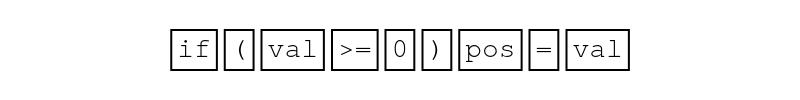
\includegraphics[scale=0.4]{./chapters/lexical.png}
  \centering
\end{figure}

\section{Análise sintática}

O próximo passo é a análise sintática, que cria uma estrutura em
árvore que captura a sintaxe do programa, descartando elementos
sintáticos como parênteses que não afetam o significado do programa.
O resultado desta fase é uma árvore sintática abstrata. Na figura
seguinte, apresentamos a árvore de sintaxe para nosso programa de exemplo.

\begin{figure}[H]
  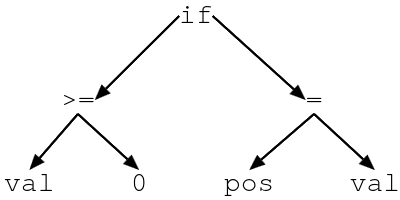
\includegraphics[scale=0.4]{./chapters/syntax-tree.png}
  \centering
\end{figure}

\section{Análise semântica}

A análise semântica completa a tarefa de determinar se o código-fonte
representa um programa válido. Frequentemente, envolve a verificação
de tipos. Informações adicionais sobre o programa podem ser coletadas
durante essa fase, como os tipos de expressões do programa. Essas
informações podem ser usadas para enriquecer a árvore sintática
abstrata. Na figura seguinte, apresentamos a árvore de sintaxe
contendo informação de tipos sobre todos os elementos do código.

\begin{figure}[H]
  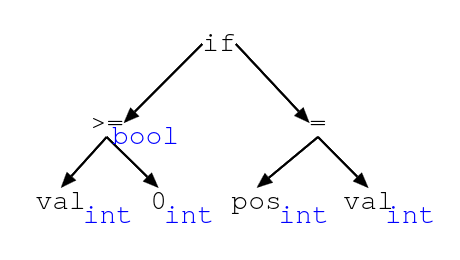
\includegraphics[scale=0.5]{./chapters/annotated-tree.png}
  \centering
\end{figure}

\section{Geração de código}

Após as etapas de análise, o compilador gera novas representações do
programa. Normalmente, há uma fase inicial de geração de código que
produz uma representação intermediária (RI) do programa. Uma fase
posterior do compilador gera o código alvo. Quando a linguagem alvo é
código assembly, essa fase é chamada de seleção de instruções.

Uma representação intermediária comum é um \emph{grafo de fluxo de
controle}. A representação como grafo de fluxo de controle do trecho
de código exemplo é apresentada na figura abaixo.

\begin{figure}[H]
  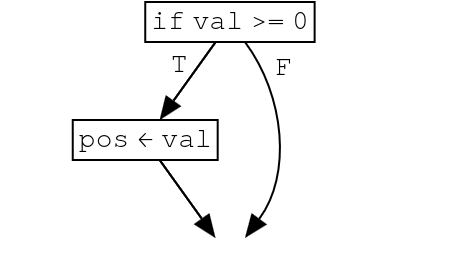
\includegraphics[scale=0.5]{./chapters/cfg.png}
  \centering
\end{figure}

Uma fase posterior da geração de código é a \emph{seleção de
instruções}, na qual a representação intermediária é traduzida em
instruções assembly. As instruções podem ser geradas como código
abstrato, no qual as variáveis são utilizadas como se fossem
registradores de hardware. Para o nosso exemplo, o resultado da
tradução para código de abstrato (x86-64) poderia ser o seguinte:

\begin{verbatim}
     cmp val, 0
     jl L1
     mov pos, val
L1:
\end{verbatim}

\section{Otimização de código}

A otimização de código é uma etapa cujo objetivo é melhorar a eficiência
de programas. Normalmente, ``melhor'' significa ``mais rápido'', embora
outros objetivos também sejam buscados, como reduzir o uso de memória
ou o consumo de energia do programa. A otimização pode ser aplicada
em praticamente todas as fases do compilador.

A otimização mais importante é a alocação de registradores, que
atribui variáveis à registradores de
hardware. Aplicar a alocação de registradores ao código assembly
acima poderia gerar o seguinte código assembly x86-64:

\begin{verbatim}
     cmp rax, 0
     jl L1
     mov rcx, rax
L1:
\end{verbatim}

Outra otimização que pode ser feita é usar uma sequência de
instruções, mais eficiente, que evite desvios.

\begin{verbatim}
cmp rax,0
cmovge rcx, rax
\end{verbatim}

\section{Visão geral de um compilador}

O compilador geralmente executa apenas uma parte da tarefa de
produzir código executável. Após gerar o código assembly para cada
uma das unidades de compilação (arquivos-fonte), um assembler é
utilizado para produzir módulos de código objeto que possuem
dependências entre si. Um linker resolve as dependências entre os
arquivos objeto e determina como modificar ou estender o código
assembly para que essas dependências sejam satisfeitas. Um loader,
frequentemente integrado ao sistema operacional, carrega então a
saída do linker na memória e produz uma imagem executável que o
processador pode interpretar.

\begin{figure}[H]
  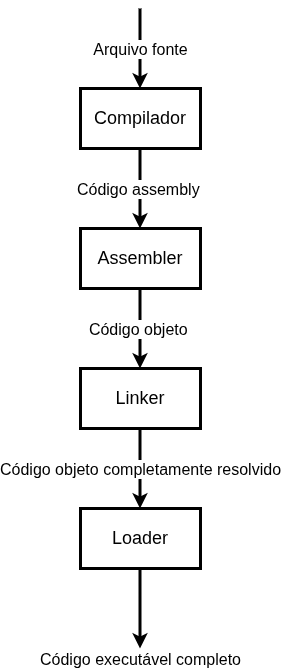
\includegraphics[scale=0.3]{./chapters/pipeline.png}
  \centering
\end{figure}

\section{Conclusão}

Neste capítulo, apresentamos uma visão geral do que é um compilador e
do desafio fundamental que ele enfrenta: traduzir programas de uma
linguagem de origem, projetada para seres humanos, para uma linguagem
de destino, otimizada para execução eficiente por hardware. Vimos
que, embora os compiladores sejam sistemas complexos, é possível
dominar essa complexidade dividindo o problema em fases menores e
mais gerenciáveis: análise léxica, sintática, semântica, geração
de código e otimização. Cada uma transformando gradualmente o
programa de sua representação original até o código de máquina final.
Ao longo deste material, exploraremos cada uma dessas fases em
detalhe, sempre buscando descrevê-las com precisão para que possamos
não apenas compreender seu funcionamento, mas também implementá-las
corretamente.

\part{Análise léxica}
\chapter{Introdução à análise léxica}

\section{Introdução}

A análise léxica é a primeira fase do processo de compilação,
responsável por ler o código-fonte como uma sequência de caracteres e
agrupá-los em tokens significativos - palavras reservadas,
identificadores, operadores, números e símbolos - enquanto remove
elementos irrelevantes como espaços em branco e comentários. Sua
importância está em transformar o texto bruto do programa em uma
representação estruturada que simplifica as fases subsequentes
(análise sintática e semântica), além de detectar erros léxicos
precocemente, como caracteres inválidos ou identificadores mal
formados, funcionando como a ``porta de entrada'' que organiza e
valida o string de entrada antes das demais etapas de um compilador /
interpretador.

Damos o nome de \textbf{token} a um componente indivisível
da sintaxe de uma linguagem. De maneira simples, o conjunto de
tokens de uma linguagem pode ser entendido como o seu alfabeto.

Antes de apresentarmos a primeira técnica de análise léxica, vamos
descrever a primeira linguagem que iremos utilizar durante o curso.

\section{A linguagem Exp}

Durante o curso de compiladores vamos implementar interpretadores e
compiladores para diversas linguagens de programação. A primeira
destas linguagens será chamada de \textbf{Exp} e está é definida pela
seguinte gramática livre de contexto.

\[
  \begin{array}{lclclclcl}
    E & \to & n & | & E + E & | & E * E & | & (E)
  \end{array}
\]

De maneira simples, a linguagem \textbf{Exp} é formada por expressões
envolvendo adição, multiplicação, parêntesis e constantes numéricas
(representadas por \textbf{n}).

O conjunto de tokens desta linguagem é dado por \{n, +, *, (, )\}. A
próxima seção vamos apresentar a implementação de um analisador
léxico ad-hoc para esta linguagem.

\section{Analisadores léxicos ad-hoc}

Um analisador léxico ad-hoc é uma implementação manual e simplificada
de um analisador léxico, construída especificamente para um problema
ou linguagem particular, sem utilizar geradores automáticos como o
Alex. Diferentemente de analisadores baseados em expressões regulares
e autômatos (tema de um próximo capítulo), o analisador ad-hoc é
tipicamente implementado através de código que processa caracteres
sequencialmente, utilizando estruturas como casamento de padrão para
identificar tokens.

O primeiro passo de nossa implementação é a definição de tipos para
representação de tokens.

\begin{minted}{haskell}
type Line = Int
type Column = Int

data Token
  = Token {
      pos :: (Line, Column)
    , lexeme :: Lexeme
    }

data Lexeme
  = TNumber Int
  | TLParen
  | TRParen
  | TPlus
  | TTimes
  | TEOF
\end{minted}

Os sinônimos \haskell{Line} e
\haskell{Column} representam a informação de linha e
coluna inicial de um token. Por sua vez, tipo
\haskell{Token} é definido como um registro contendo
dois campos: um para sua posição inicial e outro que identifica o seu
\textbf{lexema}. O tipo \haskell{Lexeme} representa
os diferentes tokens da linguagem com seus construtores:
\haskell{TNumber} representa números,
\haskell{TLParen} o abre parêntesis,
\haskell{TRParen} o fecha parêntesis,
\haskell{TPlus} o operador de adição,
\haskell{TTimes} o operador de multiplicação e
\haskell{TEOF} o final da entrada.

O próximo passo para definirmos o analisador léxico para a linguagem
\textbf{EXP} é determinar o tipo desta função. A função deverá
receber uma string de entrada e retornar uma lista de tokens. Um
possível tipo para essa função seria:

\begin{minted}{haskell}
lexer :: String -> [Token]
\end{minted}

Porém, como lidar com situações de erro? Por exemplo, qual seria o
resultado se a string possuir caracteres inválidos (por exemplo,
\textbf{a}), que não fazem parte dos possíveis tokens da linguagem? O
ideal é que o analisador retorne uma mensagem de erro apropriada.
Para isso, vamos modificar o tipo de \haskell{lexer} para:

\begin{minted}{haskell}
lexer :: String -> Either String [Token]
\end{minted}

para permitir a emissão de mensagens de erro.

A ideia do analisador léxico é percorrer a string de entrada enquanto
produz uma lista contendo os tokens encontrados até o momento.
Durante o caminhamento da entrada, vamos atualizar o \emph{estado} do
analisador léxico a cada caractere lido. O estado é definido pelo
seguinte sinônimo:

\begin{minted}{haskell}
type State = (Line, Column, String, [Token])
\end{minted}

O tipo \haskell{State} é uma quádrupla formada pela
linha atual, coluna atual, string de dígitos consecutivos encontrados
até o momento e a lista de tokens já produzidos. A cada novo
caractere processado, devemos atualizar o estado de forma apropriada.
Para isso, utilizamos a função \haskell{transition},
apresentada a seguir.

\begin{minted}{haskell}
transition :: State -> Char -> Either String State
transition state@(l, col, t, ts) c
  | c == '\n' = mkDigits state c
  | isSpace c = mkDigits state c
  | c == '+' = Right (l, col + 1, "", mkToken state (Token TPlus (l,col)) ++ ts)
  | c == '*' = Right (l, col + 1, "", mkToken state (Token TMul (l,col)) ++ ts)
  | c == '(' = Right (l, col + 1, "", mkToken state (Token TLParen (l,col)) ++ ts)
  | c == ')' = Right (l, col + 1, "", mkToken state (Token TRParen (l,col)) ++ ts)
  | isDigit c = Right (l, col + 1, c : t, ts)
  | otherwise = unexpectedCharError l col c
\end{minted}

Quando encontramos parêntesis, operadores ou dígitos simplesmente
atualizamos o estado criando um token ou adicionando o caractere de
dígito na sequência de dígitos encontrados até o momento atual. Caso
o caractere atual seja um espaço ou uma quebra de linha, tentamos
construir um token de dígitos consecutivos e atualizamos a respectiva
posição de linha / coluna. A função
\haskell{mkDigits} realiza essa tarefa. Primeiro,
verificamos se a string de dígitos encontrados é vazia, nesta
situação retornamos o estado com a informação de linha / coluna
devidamente modificada. Caso a lista de dígitos seja formada apenas
por dígitos, criamos um novo token de dígitos e atualizamos o estado
apropriadamente. Finalmente, caso nenhuma destas situações se
aplique, temos um erro.

\begin{minted}{haskell}
mkDigits :: State -> Char -> Either String State
mkDigits state@(l, col, s, ts) c
  | null s = let l' = if c == '\n' then l + 1 else l
                 col' = if isSpace c then col + 1 else col
             in (l', col', s, ts)
  | all isDigit s = let t = Token (TNumber (VInt (read $ reverse s))) (l,col)
                        l' = if c == '\n' then l + 1 else l
                        col' = if c /= '\n' && isSpace c then col + 1 else col
                    in Right (l', col', "", t : ts)
  | otherwise = unexpectedCharError l col c
\end{minted}

De posse da função de transição entre estados do analisador léxico,
podemos definir o analisador léxico como:

\begin{minted}{haskell}
lexer :: String -> Either String [Token]
lexer = finish . foldl step base
  where
    base = Right (1, 1, "", [])

    finish = either Left (Right . extract)

    step ac@(Left _) _ = ac
    step (Right state) c = transition state c

    extract (l, col, s, ts)
      | null s = reverse ts
      | otherwise = let n = read (reverse s)
                        t = Token (TNumber (VInt n))
                                  (l, col - (length s))
                    in reverse (t : ts)
\end{minted}

O valor \haskell{base} é definido como a tupla
\haskell{(1, 1, "", [])} como valor do estado inicial
do analisador léxico formado por valores iniciais de linha, coluna e
as listas de tokens e dígitos iniciais é vazia.

A função \haskell{extract} é aplicada ao estado final
do analisador léxico para tentar construir um token de dígitos a
partir da sequência de dígitos consecutivos encontrados. Finalmente,
a função \haskell{finish} realiza o casamento de
padrão no resultado do analisar léxico: caso o resultado seja um
erro, este é propagado e caso seja o estado final do analisador,
aplicamos a função \haskell{extract} para obter a
lista final de tokens da entrada.

\section{Analisadores léxicos ad-hoc: vantagens e
desvantagens}

Analisadores léxicos ad-hoc possuem a vantagem de possuir uma
implementação simples para linguagens pequenas e maior controle sobre
erros encontrados. Porém, essa técnica possui diversas desvantagens.
A primeira é que tais analisadores são difíceis de manter e extender,
além de não serem eficientes para linguagens com uma estrutura léxica
complexa. Por exemplo, como estender a implementação do analisador
ad-hoc para prover suporte a identificadores? Como dar suporte a
comentários de linha ou mesmo de blocos?

Dessa forma, esta técnica é aplicável apenas em situações em que a
simplicidade da implementação supera as vantagens de um analisadores
léxicos produzidos automaticamente a partir de expressões regulares.

\section{Conclusão}

Neste capítulo apresentamos uma introdução à análise léxica e
descrevemos uma implementação de um analisador léxico ad-hoc para uma
linguagem de programação simples. Concluímos apresentando argumentos
a favor e contra o uso deste tipo de analisadores léxicos. Nos
próximos capítulos veremos como analisadores léxios podem ser
produzidos automaticamente a partir da descrição de tokens como
expressões regulares.

\chapter{Análise léxica baseada em expressões regulares}

\section{Introdução}

No capítulo anterior, apresentamos um analisador léxico ad-hoc para
uma linguagem simples. Ao tentarmos estender a linguagem considerada
com construções simples com identificadores ou comentários,
encontraremos problemas: temos que modificar a estrutura do estado do
analisador léxico para acomodar uma string para acumular caracteres
que formam um possível identificador e modificar toda a estrutura do
analisador para lidar com comentários de linha / blocos.

Diante desta situação, temos a seguinte pergunta: existe uma forma
extensível e eficiente para a construção de analisadores léxicos?
Neste capítulo, veremos que a teoria de expressões regulares e
autômatos finitos provêem uma solução eficiente e automatizável para
a criação de analisadores léxicos.

Neste capítulo, vamos revisar a teoria de autômatos, expressões
regulares, a implementação de algoritmos e como estes podem ser
combinados para a criação de analisadores léxicos para uma
especificação de tokens usando expressões regulares.

\section{Autômatos finitos determinísticos}

Nesta seção, vamos apresentar uma implementação simples de autômatos
finitos determinísticos e de operações sobre estes.

\begin{Definition}
  Um autômato finito determinístico M pode ser entendido
  como uma quíntupla \(M = (E,\Sigma, \delta, i, F)\), em que:

  \begin{itemize}
    \item
      \(E\): conjunto finito de estados;
    \item
      \(\Sigma\): alfabeto;
    \item
      \(\delta : E \times \Sigma \to E\), função de transição;
    \item
      \(i \in E\): estado inicial;
    \item
      \(F \subseteq E\): conjunto de estados finais.
  \end{itemize}
\end{Definition}

De maneira simples, o tipo \haskell{DFA} é
parametrizado pelo tipo de estados e possui 3 campos para representar
o estado inicial (campo \haskell{start}), a função de
transição (campo \haskell{delta}) e uma função para
determinar se um estado é final ou não (campo \haskell{finals}).

\begin{minted}{haskell}
data DFA a
  = DFA {
      start :: a
    , delta :: a -> Char -> a
    , finals :: a -> Bool
    }
\end{minted}

Como um exemplo, considere o seguinte autômato que aceita palavras
que terminam em 1.

\begin{figure}[H]
  \begin{tikzpicture}[
      shorten >=1pt,
      node distance=3cm,
      on grid,
      >={Stealth[round]},
      every state/.style={draw, minimum size=12mm, font=\small},
      accepting/.style={double, double distance=1.5pt},
    ]

    \node[state, initial, initial text={}]             (q0) {$q_0$};
    \node[state, accepting, right=of q0] (q1) {$q_1$};

    \path[->]
    (q0) edge [loop above]  node {0} ()
    (q0) edge [bend left]   node [above] {1} (q1)
    (q1) edge [bend left]   node [below] {0} (q0)
    (q1) edge [loop above]  node {1} ();

  \end{tikzpicture}
  \centering
\end{figure}

Esse mesmo autômato pode ser representado pelo seguinte valor em Haskell:

\begin{minted}{haskell}
endsWithOne :: DFA Bool
endsWithOne = DFA False transition id
    where
        transition False '0' = False
        transition False '1' = True
        transition True  '0' = False
        transition True  '1' = True
        transition _ _ = False
\end{minted}

Aqui representamos o conjunto de estados utilizando o tipo
\haskell{Bool}. O estado inicial é codificado por
\haskell{False} e o estado final por
\haskell{True}. A função de transição é representada
por casamento de padrão sobre o estado e o caractere processado. A
função para identificar o estado final é a função identidade,
\haskell{id}.

O cálculo do estado em que a computação de uma string termina em um
AFD é feita percorrendo a string utilizando a função de transição de
forma direta:

\begin{minted}{haskell}
deltaStar :: DFA a -> String -> a
deltaStar m = foldl (delta m) (start m)
\end{minted}

que permite a definição direta de uma função para verificar se uma
palavra pertence ou não a linguagem descrita por um autômato por
testar se o estado retornado por \haskell{deltaStar} é final.

\begin{minted}{haskell}
accept :: DFA a -> String -> Bool
accept m s = finals m (deltaStar m s)
\end{minted}

Evidentemente, em analisadores léxicos devemos utilizar
\textbf{autômatos mínimos}, visto que estes evitam a utilização de
espaço desnecessário por utilizar a menor quantidade possível para
seu conjunto de estados. A implementação de algoritmos de minimização
está disponível no repositório de código associado a este material. O
leitor interessado pode consultar esses detalhes on-line.

\section{Autômatos finitos não determinísticos}

Nesta seção, vamos apresentar uma implementação simples de autômatos
finitos não determinísticos e de operações sobre estes. A seguir,
apresentamos a descrição formal de autômatos não determinísticos.

\begin{Definition}
  Um autômato finito não determinístico M pode ser
  entendido como uma quíntupla \(M = (E,\Sigma, \delta, I, F)\), em que:

  \begin{itemize}
    \item
      \(E\): conjunto finito de estados;
    \item
      \(\Sigma\): alfabeto;
    \item
      \(\delta : E \times \Sigma \to \mathcal{P}(E)\), função de transição;
    \item
      \(I \subseteq E\): conjunto de estados iniciais;
    \item
      \(F \subseteq E\): conjunto de estados finais.
  \end{itemize}
\end{Definition}

Para representação de um autômato não determinístico, vamos
representar de maneira explícita o conjunto de estados do autômato. A
função de transição retorna um conjunto de estados para representar a
possibilidade dos diversos resultados de uma transição em um AFN.

\begin{minted}{haskell}
data NFA a
  = NFA {
      numberOfStates :: Int
    , nfaStart :: Set a
    , nfaDelta :: a -> Char -> Set a
    , nfaFinals :: Set a
    }
\end{minted}

Como um exemplo, considere o seguinte AFN que aceita a linguagem de
palavras que terminam em 00:
\begin{figure}[H]
  \begin{tikzpicture}[
      shorten >=1pt,
      node distance=3cm,
      on grid,
      >={Stealth[round]},
      every state/.style={draw, minimum size=12mm, font=\small},
      accepting/.style={double, double distance=1.5pt},
    ]

    \node[state, initial, initial text={}]                (q0) {$q_0$};
    \node[state, right=of q0]           (q1) {$q_1$};
    \node[state, accepting, right=of q1] (q2) {$q_2$};

    \path[->]
    (q0) edge [loop above] node {0, 1} ()
    (q0) edge              node [above] {0} (q1)
    (q1) edge              node [above] {0} (q2);

  \end{tikzpicture}
  \centering
\end{figure}

este é representado pelo seguinte valor do tipo \haskell{NFA Int}:

\begin{minted}{haskell}
endsWith00 :: NFA Int
endsWith00
    = NFA 3 (Set.singleton 0)
            (\ s c -> case (s,c) of
                        (0, '0') -> Set.fromList [0,1]
                        (0, '1') -> Set.singleton 0
                        (1, '0') -> Set.singleton 2
                        _        -> Set.empty)
            (Set.singleton 2)
\end{minted}

Note que a função de transição é codificada por um par formado por um
estado e o caractere a ser processado pela transição. Os conjuntos de
estados iniciais e finais são representados utilizando a função
\haskell{Set.singleton} que cria um conjunto unitário
com o elemento fornecido como argumento. A definição de aceitação de
uma palavra é similar à de AFDs e está implementada no código de
suporte deste material.

A definição seguinte revisa a equivalência entre AFNs e AFDs.

\begin{Definition}
  Seja $M = (E,\Sigma, \delta, I, F)$ um autômato
  finito não determinístico qualquer. O AFD equivalente a $M$ é
  $M' = (\mathcal{P}(E),\Sigma,\delta',I,F')$, em que:

  \begin{itemize}
    \item
      \(\delta' : \mathcal{P}(E) \times \Sigma \to \mathcal{P}(E)\),
      função de transição;
    \item
      \(I \in \mathcal{P}(E)\): estado inicial;
    \item
      \(F' =\{X \,|\, X \cap F \neq \emptyset\}\): conjunto de estados finais.
  \end{itemize}

  De maneira simples, no AFD equivalente cada estado representa um
  conjunto de estados do AFN. O estado inicial do AFD é apenas o
  conjunto de estados iniciais do AFN e o conjunto de estados finais
  é qualquer conjunto de estados que possui algum estado final do AFN.
\end{Definition}

A partir da definição anterior, podemos codificar uma função que
transforma um AFN qualquer em um AFD equivalente.

\begin{minted}{haskell}
subset :: Ord a => NFA a -> DFA (Set a)
subset m
  = DFA {
      start  = nfaStart m
    , delta  = \ es c ->
        Set.unions (map (flip (nfaDelta m) c) (Set.elems es))
    , finals = \ es -> not (disjoint es (nfaFinals m))
    }
\end{minted}

Observe que a função mostra que se o AFN possui estados de tipo
\haskell{a}, o AFD equivalente terá estados de tipo
\haskell{Set a}, isto é, conjuntos de estados de tipo
\haskell{a}. O estado inicial do AFD é definido como
o estado inicial do AFN, \haskell{nfaStart m}.
Estados finais são definidos por uma função que verifica se o
argumento possui algum estado final do AFN\footnote{A função
  \haskell{disjoint} retorna verdadeiro se a interseção
entre dois conjuntos é vazia.}.

\section{Expressões regulares}

Uma abordagem mais declarativa para análise léxica consiste em
definir os tokens válidos usando expressões regulares e, em seguida,
sintetizar automaticamente o analisador léxico a partir dessas
expressões regulares. Essa abordagem é simples e tem maior
probabilidade de resultar em código eficiente e de fácil manutenção.

Para iniciar, vamos rever a definição da sintaxe de expressões
regulares e de sua semântica.

\begin{Definition}
  Expressões regulares são definidas pela seguinte
  gramática livres de contexto: \[
    \begin{array}{l}
      e \to \emptyset\,|\,\lambda\,|\,a\,|\,e e\,|\,e + e\,|\,e^\star
    \end{array}
  \] Uma expressão regular \(e\) denota um conjunto de strings
  chamado linguagem de \(e\), escrita \(L(e)\), que é definida
  recursivamente como: \[
    \begin{array}{lcl}
      L(\emptyset) & = & \emptyset\\
      L(\lambda) & = & \{\lambda\}\\
      L(a)        & = & \{a\}\\
      L(e_1 e_2)  & = & L(e_1)L(e_2)\\
      L(e_1 + e_2) & = & L(e_1) \cup L(e_2)\\
      L(e^\star)  & = & L(e)^\star
    \end{array}
  \]
\end{Definition}

Existem diversas maneiras para converter uma expressão regular em um
autômato equivalente. Primeiro, vamos revisar uma abordagem que
produz um AFN equivalente por recursão sobre a estrutura da expressão regular.

\begin{Definition}[Construção de Thompson]
  Seja \(e\) uma
  expressão regular arbitrária. O AFN equivalente a \(e\), \(M\), é
  definido por recursão sobre a estrutura de \(e\):

  Caso \(e = \emptyset\): O AFN \(M\) equivalente é

  \begin{figure}[H]
    \begin{tikzpicture}[
        shorten >=1pt,
        node distance=3cm,
        on grid,
        >={Stealth[round]},
        every state/.style={draw, minimum size=12mm, font=\small},
      ]
      \node[state, initial, initial text={}] (q0) {$q_0$};
    \end{tikzpicture}
    \centering
  \end{figure}

  Caso $e = \lambda$: O AFN \(M\) equivalente é
  \begin{figure}[H]
    \begin{tikzpicture}[
        shorten >=1pt,
        node distance=3cm,
        on grid,
        >={Stealth[round]},
        every state/.style={draw, minimum size=12mm, font=\small},
      ]
      \node[state, initial,accepting, initial text={}] (q0) {$q_0$};
    \end{tikzpicture}
    \centering
  \end{figure}

  Caso \(e = a\): O AFN \(M\) equivalente é

  \begin{figure}[H]
    \begin{tikzpicture}[
        shorten >=1pt,
        node distance=3cm,
        on grid,
        >={Stealth[round]},
        every state/.style={draw, minimum size=12mm, font=\small},
        accepting/.style={double, double distance=1.5pt},
      ]

      % Estados
      \node[state, initial, initial text={}]                (q0) {$q_0$};
      \node[state, accepting, right=of q0] (q1) {$q_1$};

      % Transição
      \path[->]
      (q0) edge node [above] {a} (q1);

    \end{tikzpicture}
    \centering
  \end{figure}

  Caso \(e = e_1 + e_2\): O AFN \(M\) equivalente é

  \begin{figure}[H]
    \begin{tikzpicture}[
        shorten >=1pt,
        node distance=2.5cm,
        on grid,
        >={Stealth[round]},
        every state/.style={draw, minimum size=12mm, font=\small},
        accepting/.style={double, double distance=1.5pt},
      ]

      \node[state, initial, initial text={}] (q0) {$q_0$};

      \node[state, above right=2cm and 2.5cm of q0] (q1) {$q_1$};
      \node[state, right=of q1]                      (q2) {$q_2$};

      \node[state, below right=2cm and 2.5cm of q0] (q3) {$q_3$};
      \node[state, right=of q3]                      (q4) {$q_4$};

      \node[state, accepting, below right=2cm and 2.5cm of q2] (qf) {$q_f$};

      \begin{pgfonlayer}{background}
        \node[ellipse, draw=blue!70, fill=blue!10, thick,
          inner sep=8pt, fit=(q1)(q2),
        label={[blue!70, font=\footnotesize]above:$N(e_1)$}] {};
        \node[ellipse, draw=red!70, fill=red!10, thick,
          inner sep=8pt, fit=(q3)(q4),
        label={[red!70, font=\footnotesize]below:$N(e_2)$}] {};
      \end{pgfonlayer}

      \path[->]
      (q0) edge node [above left]  {$\lambda$} (q1)
      (q0) edge node [below left]  {$\lambda$} (q3)
      (q1) edge [blue!70, thick] node [above, text=black] {$e_1$} (q2)
      (q3) edge [red!70, thick]  node [above, text=black] {$e_2$} (q4)
      (q2) edge node [above right] {$\lambda$} (qf)
      (q4) edge node [below right] {$\lambda$} (qf);

    \end{tikzpicture}
    \centering
  \end{figure}

  em que N($e_1$) é o AFN equivalente a $e_1$ e N($e_2$)
  é o AFN equivalente a $e_2$.

  Caso \(e = e_1 e_2\): O AFN \(M\) equivalente é

  \begin{figure}[H]
    \begin{tikzpicture}[
        shorten >=1pt,
        node distance=3cm,
        on grid,
        >={Stealth[round]},
        every state/.style={draw, minimum size=12mm, font=\small},
        accepting/.style={double, double distance=1.5pt},
      ]

      \node[state, initial, initial text={}]    (q0) {$q_0$};
      \node[state, right=of q0] (q1) {$q_1$};

      \node[state, right=of q1] (q2) {$q_2$};
      \node[state, accepting, right=of q2] (q3) {$q_3$};

      \begin{pgfonlayer}{background}
        \node[ellipse, draw=blue!70, fill=blue!10, thick,
          inner sep=10pt, fit=(q0)(q1),
        label={[blue!70, font=\footnotesize]above:$N(e_1)$}] {};
        \node[ellipse, draw=red!70, fill=red!10, thick,
          inner sep=10pt, fit=(q2)(q3),
        label={[red!70, font=\footnotesize]above:$N(e_2)$}] {};
      \end{pgfonlayer}

      \path[->]
      (q0) edge [blue!70, thick]  node [above, text=black] {$e_1$} (q1)
      (q1) edge                   node [above] {$\lambda$}      (q2)
      (q2) edge [red!70, thick]   node [above, text=black] {$e_2$} (q3);
    \end{tikzpicture}
    \centering
  \end{figure}

  em que N($e_1$) é o AFN equivalente a $e_1$ e N($e_2$) é o
  AFN equivalente a $e_2$.

  Caso $e = e_1^\star$: O AFN \(M\) equivalente é

  \begin{figure}[H]
    \begin{tikzpicture}[
        shorten >=1pt,
        node distance=3cm,
        on grid,
        >={Stealth[round]},
        every state/.style={draw, minimum size=12mm, font=\small},
        accepting/.style={double, double distance=1.5pt},
      ]

      \node[state, initial, initial text={}] (q0) {$q_0$};

      \node[state, right=of q0]  (q1) {$q_1$};
      \node[state, right=of q1]  (q2) {$q_2$};

      \node[state, accepting, right=of q2] (qf) {$q_f$};

      \begin{pgfonlayer}{background}
        \node[ellipse, draw=violet!70, fill=violet!10, thick,
          inner sep=10pt, fit=(q1)(q2),
        label={[violet!70, font=\footnotesize]above:$N(e_1)$}] {};
      \end{pgfonlayer}

      \path[->]
      (q0) edge node [above] {$\lambda$} (q1)
      (q1) edge [violet!70, thick] node [above, text=black] {$e_1$} (q2)
      (q2) edge node [above] {$\lambda$} (qf)
      (q2) edge [bend left=50] node [below] {$\lambda$} (q1)
      (q0) edge [bend left=50] node [above] {$\lambda$} (qf);

    \end{tikzpicture}
    \centering
  \end{figure}

  em que N($e_1$) é o AFN equivalente a $e_1$.
\end{Definition}

\section{Gerando AFNs a partir de ERs.}

Nesta seção, vamos apresentar uma implementação Haskell da construção
de Thompson. O primeiro passo é representar expressões regulares
utilizando um tipo de dados Haskell, conforme a seguir:

\begin{minted}{haskell}
data Regex
  = Empty
  | Lambda
  | Chr Char
  | Regex :+: Regex
  | Regex :@: Regex
  | Star Regex
\end{minted}

Para a criação de AFNs a partir da expressão regular, temos que
definir qual tipo representará os estados do AFN. Por questão de
simplicidade, vamos utilizar o tipo \haskell{Int}
para representar estados. Dessa forma, os AFNs produzidos terão tipo
\haskell{NFA Int}.

Iniciamos apresentando o AFN equivalente a expressão regular
\haskell{Empty}:

\begin{minted}{haskell}
emptyNFA :: NFA Int
emptyNFA
  = NFA 0 Set.empty (\ _ _ -> Set.empty) Set.empty
\end{minted}

que consiste de um AFN que não possui estados e nem transições. Dessa
forma, aceita a linguagem vazia\footnote{Optamos por não representar
  como um AFN de um único estado não final para reduzir o número de
estados que seriam considerados inúteis posteriormente.}. O AFN que
aceita a linguagem formada apenas pela palavra vazia é:

\begin{minted}{haskell}
lambdaNFA :: NFA Int
lambdaNFA
  = NFA 1 one (\ _ _ -> Set.empty) one
    where
      one = Set.singleton 1
\end{minted}

que denota um AFN de um único estado inicial e final, sem transições.
A função \haskell{chrNFA} constrói um AFN que aceita
um caractere recebido como argumento.

\begin{minted}{haskell}
chrNFA :: Char -> NFA Int
chrNFA c
  = NFA 2 zero f one
    where
      zero = Set.singleton 0
      one = Set.singleton 1
      err = Set.empty
      f 0 x = if c == x then one
              else err
      f _ _ = err
\end{minted}

Este AFN possui dois estados: 0, que é inicial e não final e 1 que é
final. A função de transição produz como resultado um conjunto vazio,
exceto quando a origem da transição é o estado 0 e o caractere
processado é igual a \haskell{c}, que é o argumento
de \haskell{chrNFA}.

Antes de apresentar funções para produzir AFNs para união,
concatenação e fecho de Kleene, devemos garantir que AFNs não possuam
estados com o mesmo \textbf{nome} (i.e.~mesmo valor de tipo
\haskell{Int}). Para resolver esse problema, vamos
definir uma função que soma um valor \haskell{n} a
cada elemento de um conjunto de inteiros.

\begin{minted}{haskell}
shift :: Int -> Set Int -> Set Int
shift n = Set.fromAscList . map (+ n) . Set.toAscList
\end{minted}

A função \haskell{shift} converte um conjunto de
entrada (tipo \haskell{Set Int}) para uma lista de
inteiros, usando \haskell{Set.toAscList}, e então
soma \haskell{n} a cada elemento da lista produzida
para convertê-la em um conjunto novamente utilizando a função
\haskell{Set.fromAscList}.

A função que calcula o AFN que aceita a união da linguagem de dois
AFNs fornecidos como argumentos é definida como:

\begin{minted}{haskell}
unionNFA :: NFA Int -> NFA Int -> NFA Int
unionNFA m1 m2
  = NFA {
      numberOfStates = n1 + n2
    , nfaStart = Set.union (nfaStart m1) (shift n1 (nfaStart m2))
    , nfaDelta = f
    , nfaFinals = Set.union (nfaFinals m1) (shift n1 (nfaFinals m2))
    }
    where
      n1 = numberOfStates m1
      n2 = numberOfStates m2
      f s c = if s < n1 then nfaDelta m1 s c
              else shift n1 (nfaDelta m2 (s - n1) c)
\end{minted}

A função \haskell{unionNFA} implementa a união de
dois AFNs combinando seus conjuntos de estados de forma disjunta.
Para evitar colisões, ela preserva a estrutura do primeiro autômato
\haskell{m1} e utiliza uma função de deslocamento
\haskell{shift} para renomear os estados do segundo
(\haskell{m2}), garantindo que todos os novos estados
sejam únicos. O resultado é um novo NFA onde os estados iniciais, as
transições e os estados de aceitação são a união das partes
correspondentes de ambos os autômatos originais, permitindo que o AFN
resultante reconheça a linguagem composta pela união das linguagens
aceitas por \haskell{m1} e \haskell{m2}.

A seguir, apresentamos a função que calcula o AFN que aceita
concatenação das linguagem aceitas por dois AFNs fornecidos como argumento.

\begin{minted}{haskell}
concatNFA :: NFA Int -> NFA Int -> NFA Int
concatNFA m1 m2
  = NFA {
      numberOfStates = n1 + n2
    , nfaStart = newStart
    , nfaDelta = newDelta
    , nfaFinals = newFinals
    }
    where
      n1 = numberOfStates m1
      n2 = numberOfStates m2
      start1 = nfaStart m1
      final1 = nfaFinals m1
      final2 = nfaFinals m2
      newStart = if disjoint start1 final1
                 then start1
                 else Set.union start1 (shift n1 final1)
      newFinals = shift n1 final2
      newDelta e c = if e < n1 then
                       if disjoint (nfaDelta m1 e c) final1
                       then nfaDelta m1 e c
                       else Set.union (nfaDelta m1 e c) (shift n1 start2)
                     else shift n1 (nfaDelta m2 (e - n1) c)
\end{minted}

Assim como na construção da união de dois AFNs, utilizamos a função
\haskell{shift} para garantir que estados de cada um
dos AFNs de entrada não possuam o mesmo nome. Para isso, utilizamos o
renomeamento nas definições da função de transição e nos conjuntos de
estados iniciais e finais. A implementação da função de transição
\haskell{newDelta} decide o fluxo da computação com
base no índice do estado atual: se o estado pertence ao primeiro AFN
(\haskell{e < n1}), a função executa a transição
original de \haskell{m1}, mas utiliza a verificação
\haskell{disjoint} para identificar se o destino
atinge um estado de aceitação; em caso positivo, ela funde esse
destino aos estados iniciais para permitir o início imediato do
processamento da segunda linguagem, simulando a conexão entre os
autômatos sem recorrer a transições vazias. Caso o estado já pertença
ao segundo AFN (\haskell{e >= n1}), a função
simplesmente associa a transição original de
\haskell{m2} para o novo intervalo de índices
utilizando \haskell{shift}, garantindo que, uma vez
iniciada a segunda parte da cadeia, o autômato permaneça restrito a
\haskell{m2}.

A função \haskell{starNFA} implementa o fecho de
Kleene ao produzir um AFN, a partir de \haskell{m1},
que aceita zero ou mais repetições da linguagem original, sem
adicionar novos estados. Para permitir a aceitação da string vazia e
o reinício do ciclo, a função redefine os estados de aceitação
(\haskell{nfaFinals}) como sendo os próprios estados
iniciais (\haskell{nfaStart m1}) e modifica a função
de transição (\haskell{newDelta}): sempre que uma
transição original de \haskell{m1} atingiria um
estado final, ela é inclui os estados iniciais usando
\haskell{Set.union}. Esse detalhe cria um laço que
permite ao autômato processar múltiplas palavras consecutivas,
tratando o alcance de um estado final como um gatilho para reiniciar
a computação a partir de algum dos estados iniciais.

\begin{minted}{haskell}
starNFA :: NFA Int -> NFA Int
starNFA m1
  = NFA {
      numberOfStates = numberOfStates m1
    , nfaStart = nfaStart m1
    , nfaDelta = newDelta
    , nfaFinals = nfaStart m1
    }
    where
      newDelta e c
        = let r = nfaDelta m1 e c
          in if disjoint r (nfaFinals m1)
             then r
             else Set.union r (nfaStart m1)
\end{minted}

De posse de todas essas funções auxiliares, a conversão de uma
expressão regular em um AFN equivalente é definida por recursão sobre
a estrutura da expressão:

\begin{minted}{haskell}
thompson :: Regex -> NFA Int
thompson Empty = emptyNFA
thompson Lambda = lambdaNFA
thompson (Chr c) = chrNFA c
thompson (e1 :+: e2)
  = unionNFA (thompson e1) (thompson e2)
thompson (e1 :@: e2)
  = concatNFA (thompson e1) (thompson e2)
thompson (Star e1)
  = starNFA (thompson e1)
\end{minted}

Especificações léxicas de uma linguagem são feitas utilizando
diversas expressões regulares. A função a seguir, combina as
implementações descritas até o momento para produzir o AFD
equivalente a uma lista de expressões regulares:

\begin{minted}{haskell}
lexer :: [Regex] -> DFA (Set Int)
lexer = subset . foldr unionNFA emptyNFA . map thompson
\end{minted}

Primeiro, obtemos um AFN equivalente para cada expressão usando a
função \haskell{thompson}. Em seguida, realizados a
união de todos os AFNs produzidos utilizando a função
\haskell{unionNFA}. Finalmente, obtemos o AFD
equivalente chamando a função \haskell{subset} sobre
o resultado dos passos anteriores.

\section{Critério do maior prefixo}

Autômatos fornecem um maneira eficiente e fundamentada para a criação
de analisadores léxicos. Porém, a mera aceitação de um prefixo da
entrada é suficiente para que um analisador produza um token? Para
entender considere o seguinte trecho de código:

\begin{minted}{java}
if (x > 0) ift = x + 1;
\end{minted}

Como diferenciar o identificador \haskell{ift} da
palavra reservada \haskell{if}? A ideia é que
analisadores léxicos sempre busquem aceitar o \textbf{maior prefixo}
possível. Esse critério é necessário para evitar ambiguidades
semânticas e garantir que a análise reflita a intenção real da
linguagem. Sem esse critério, o analisador léxico poderia fragmentar
precocemente sequências de caracteres que possuem um significado
específico quando combinadas, gerando múltiplos tokens genéricos em
vez de um único token. Com isso, o compilador assegura que
identificadores, palavras-reservadas e operadores compostos sejam
interpretados de forma atômica e correta dentro do contexto gramatical.

Mas isso nos leva a seguinte pergunta: Como reconhecer o maior
prefixo utilizando um AFD? A função a seguir, permite que um AFD de
argumento reconheça o maior prefixo de uma string de entrada.

\begin{minted}{haskell}
longest :: DFA a -> String -> Maybe String
longest m = combine . foldl step (Just "", Nothing, start m)
  where
    step (Just pre, Nothing, e) c
      | finals m (delta m e c)
          = ( Just (c : pre)
            , Just (c : pre)
            , delta m e c)
      | otherwise
          = ( Just (c : pre)
            , Nothing
            , delta m e c)
    step (Just pre, Just pre', e) c
      | finals m (delta m e c)
          = ( Just (c : pre)
            , Just (c : pre')
            , delta m e c)
      | otherwise = ( Nothing
                    , Just pre'
                    , delta m e c)
    step (Nothing, val, e) c = ( Nothing
                               , val
                               , delta m e c)

    combine (_, val, _) = reverse <$> val
\end{minted}

A função \haskell{longest} busca identificar o maior
prefixo de uma string aceita por AFD, percorrendo a entrada enquanto
mantém um acumulador representado como uma tripla formada por:

\begin{itemize}
  \item
    Prefixo atual sendo processado
  \item
    Último prefixo válido (aceito pelo DFA) encontrado até o momento
  \item
    Estado atual do autômato.
\end{itemize}

A lógica de atualização do acumulador é feita pela função
\haskell{step} que lida com três situações: ela
acumula caracteres no prefixo atual enquanto for possível estendê-lo,
salva essa string como o ``melhor resultado'' sempre que atinge um
estado final (\haskell{finals}) e, caso o caminho se
torne inválido para futuras aceitações (indicado pelo valor
\haskell{Nothing} no primeiro elemento da tupla),
interrompe a atualização do prefixo em progresso mas preserva a maior
correspondência já registrada. Ao final, a função
\haskell{combine} recupera esse maior prefixo
armazenado e inverte a ordem da string (corrigindo a inversão causada
pela construção da lista) para retornar a string resultante.

\section{Derivadas de expressões regulares}

A geração de analisadores léxicos baseados na construção de Thompson
é útil para o reconhecimento de expressões regulares em um
compilador, visto que a especificação do token não se altera. No
entanto, expressões regulares são frequentemente usadas em outros
contextos em que a pré-compilação em um AFD não compensa o custo.
Infelizmente, bibliotecas comuns de expressões regulares, como as
utilizadas por Java, Perl e Javascript, apresentam desempenho
exponencial no pior caso, pois empregam backtracking para lidar com o
operador de união.

Uma técnica alternativa consiste em interpretar diretamente a
expressão regular à medida que a entrada é analisada, usando
derivadas de expressões regulares, uma técnica elegante desenvolvida
por Janus Brzozowski. A ideia é que, para qualquer expressão regular
e símbolo de entrada, podemos calcular a expressão regular que aceita
o restante da entrada após o símbolo de entrada ter sido consumido.
Usamos a notação \(\partial(e,a)\) para representar a derivada da
expressão regular \(e\) com respeito ao símbolo de entrada \(a\).

Antes de apresentar a definição de derivadas propriamente ditas,
precisamos de um conceito auxilar: a noção de anulabilidade. Dizemos
que uma expressão regular é \textbf{anulável} se \(\lambda \in
L(e)\). Esse conceito é definido a seguir.

\begin{Definition}
  Dizemos que uma expressão regular é \textbf{anulável}
  se \(\nu(e) = \top\), em que \(\nu(e)\) é definido por recursão
  sobre a estrutura da expressão da seguinte maneira:

  \[
    \begin{array}{lcl}
      \nu(\emptyset) & = & \bot\\
      \nu(\lambda)   & = & \top\\
      \nu(a)          & = & \bot\\
      \nu(e_1 e_2)    & = & \nu(e_1) \land \nu(e_2)\\
      \nu(e_1 + e_2)  & = & \nu(e_1) \lor \nu(e_2)\\
      \nu(e_1^\star) & = & \top\\
    \end{array}
  \]
\end{Definition}

As três primeiras equações mostram que o conjunto vazio não é
anulável, que \(\lambda\) é anulável e que um símbolo não é
considerado anulável. Uma concatenação é anulável somente se ambas as
suas sub-expressões são anuláveis e a união é considerada anulável se
qualquer uma de suas sub-expressões o for anulável. Finalmente, uma
expressão envolvendo o fecho de Kleene é sempre anulável.

Utilizando o conceito de anulabilidade, podemos definir a derivada de
expressões regulares.

\begin{Definition}[Derivada de uma expressão regular]
  Seja \(e\) uma expressão regular qualquer e \(a\in
  \Sigma\). A derivada de \(e\) com respeito a \(a\) é definida como:

  \[
    \begin{array}{lcl}
      \partial(\emptyset,a) & = & \emptyset\\
      \partial(\lambda, a)  & = & \emptyset\\
      \partial(b, a)         & = & \left\{
        \begin{array}{ll}
          \lambda & \textrm{se }a = b \\
          \emptyset & \textrm{caso contrário}
        \end{array}
        \right . \\
        \partial(e_1 + e_2, a) & = & \partial(e_1,a) + \partial(e_2,a)\\
        \partial(e_1 e_2, a)   & = & \left\{
          \begin{array}{ll}
            \partial(e_1, a) e_2 + \partial(e_2, a) & \textrm{se
            }\nu(e_1) = \top\\
            \partial(e_1,a) e_2 & \textrm{caso contrário}
          \end{array}
          \right .\\
          \partial(e_1^\star)   & = & \partial(e_1,a)e_1^\star
        \end{array}
      \]
    \end{Definition}

    A definição da derivada de uma expressão regular em relação a um
    símbolo \$\$ é apresentada de forma recursiva. Para os casos
    base: a derivada da expressão vazia \(\emptyset\) ou da palavra
    vazia \(\lambda\) em relação a qualquer símbolo resulta em
    \(\emptyset\), pois não é possível consumir um caractere a partir
    delas. No caso de um símbolo \(b\), a derivada retorna
    \(\lambda\) se o símbolo consumido \(a\) for igual a \(b\)
    (indicando que o caractere esperado foi encontrado e a expressão
    se reduz à palavra vazia), ou \(\emptyset\) caso contrário. Para
    a união \(e_1 + e_2\), a derivada é simplesmente a união das
    derivadas de cada subexpressão. No caso da concatenação \(e_1
    e_2\), a definição se desdobra: se \(e_1\)\hspace{0pt} for
    anulável (ou seja, pode reconhecer a palavra vazia), a derivada é
    a união entre a concatenação da derivada de \(e_1\) com \(e_2\) e
    a derivada de \(e_2\)\hspace{0pt}; caso contrário, é apenas a
    derivada de \(e_1\)\hspace{0pt} concatenada com \(e_2\). Por fim,
    para o fecho de Kleene \(e^\star\), a derivada é a concatenação
    da derivada de \(e\)\hspace{0pt} com a própria estrela
    \(e^\star\), permitindo que a expressão continue reconhecendo
    múltiplas repetições.

    Para obter um autômato finito determinístico (AFD) a partir de
    uma expressão regular utilizando derivadas, podemos construir os
    estados do autômato como as próprias expressões regulares que
    surgem durante o processo de derivação. A ideia fundamental é
    que, partindo da expressão regular original \(e_0\)\hspace{0pt},
    podemos calcular sua derivada em relação a cada símbolo do
    alfabeto, obtendo novas expressões que representam o estado após
    consumir aquele símbolo. Este processo é repetido para cada nova
    expressão gerada, até que nenhuma nova expressão seja produzida,
    garantindo que o conjunto de estados seja finito.

    \begin{Definition}
      Seja \(e\) uma expressão regular qualquer. O AFD
      equivalente a \(e\) é \(M = (E, \Sigma, \delta, i, F)\), em
      que:
      \begin{itemize}
        \item \(E\): é o conjunto de todas as derivadas para a
          expressão \(e\).
        \item \(\Sigma\): alfabeto de entrada
        \item \(\delta\): função de transição, representada pela própria
          derivada: \(\delta(e,a) = \partial(e,a)\).
        \item \(F = \{e_1 \,|\,
          \nu(e_1) = \top\}\), isto é, consideramos como estados finais
          as expressões regulares anuláveis.
      \end{itemize}
    \end{Definition}

    Um ponto crucial nesta construção é o fato de que o conjunto de
    derivadas de uma expressão é \textbf{finito}. Porém, esse fato é
    verdade apenas se considerarmos algumas simplificações,
    apresentadas a seguir:
    \[
      \begin{array}{ccc}
        e_1 + \emptyset \equiv e_1 &
        \emptyset + e_2 \equiv e_2 &
        e_1\emptyset \equiv \emptyset \\
        \emptyset e_2 \equiv \emptyset &
        e_1 \lambda\equiv e_1 &
        \lambda e_2 \equiv e_2 \\
        \lambda^\star \equiv \lambda &
        \emptyset^\star \equiv \lambda &
        (e^\star)^\star \equiv e^\star
      \end{array}
    \]

    Considerando essas simplificações, é demonstrado que sempre
    obteremos um conjunto finito de derivadas a partir de uma
    expressão regular qualquer.

    \section{Implementação em Haskell}

    De posse das definições, podemos implementar a obtenção de um AFD
    a partir de uma expressão regular de forma direta. Primeiro,
    vamos definir uma função para determinar se uma expressão é ou não anulável.

\begin{minted}{haskell}
nullable :: Regex -> Bool
nullable Empty = False
nullable Lambda = True
nullable (Chr _) = False
nullable (e1 :+: e2) = nullable e1 || nullable e2
nullable (e1 :@: e2) = nullable e1 && nullable e2
nullable (Star _) = True
\end{minted}

    Observe que a implementação é uma tradução direta da notação
    matemática para código Haskell. Em seguida, apresentamos funções
    para realizar as simplificações da união, concatenação e fecho de
    Kleene. Cada uma destas funções realiza as simplificações
    apresentadas anteriormente.

\begin{minted}{haskell}
(.+.) :: Regex -> Regex -> Regex
Empty .+. e' = e'
e .+. Empty  = e
e .+. e'     = e :+: e'

(.@.) :: Regex -> Regex -> Regex
Empty .@. _ = Empty
_ .@. Empty = Empty
Lambda .@. e' = e'
e .@. Lambda = e
e .@. e' = e :@: e'

star :: Regex -> Regex
star Empty = Lambda
star (Star e) = e
star e = Star e
\end{minted}

    De posse destas simplificações e do teste de anulabilidade, a
    implementação da operação de derivada é apenas a tradução da
    notação matemática para código Haskell.

\begin{minted}{haskell}
deriv :: Char -> Regex -> Regex
deriv _ Empty  = Empty
deriv _ Lambda = Empty
deriv a (Chr b)
  | a == b = Lambda
  | otherwise = Empty
deriv a (e1 :+: e2)
  = deriv a e1 .+. deriv a e2
deriv a (e1 :@: e2)
  | nullable e1 = deriv a e1 .@. e2 .+. deriv a e2
  | otherwise   = deriv a e1 .@. e2
deriv a (Star e1)
  = deriv a e1 .@. (star e1)
\end{minted}

    Para construção do AFD utilizando derivadas, precisamos obter o
    conjunto de todas as derivadas de uma expressão regular. A função
    \haskell{enumerateDerivs} implementa um algoritmo
    para enumerar todas as expressões regulares alcançáveis a partir
    de uma expressão inicial (\haskell{initial})
    através da aplicação sucessiva da operação de derivada em relação
    aos símbolos do alfabeto.

\begin{minted}{haskell}
enumerateDerivs :: Regex -> [Regex]
enumerateDerivs initial = go [initial] [initial]
  where
    go [] acc = acc
    go (state:rest) acc =
        let chars = symbols initial
            newStates = nub [deriv c state | c <- chars]
            unseen = filter (`notElem` acc) newStates
        in go (rest ++ unseen) (acc ++ unseen)
\end{minted}

    A função \haskell{enumerateDerivs} realiza uma
    busca sistemática em largura sobre o espaço de estados
    (expressões regulares), utilizando duas listas: a primeira
    (state:rest) funciona como uma fila de estados a serem
    processados, enquanto a segunda (acc) acumula todos os estados já
    visitados. Para cada estado atual, a função obtém todos os
    símbolos do alfabeto a partir da expressão inicial (usando
    \haskell{symbols initial}), calcula a derivada
    para cada um deles com \haskell{deriv c state}, e
    remove duplicidades com \haskell{nub}. As novas
    expressões geradas que ainda não estão no acumulador

    (\haskell{filter (notElem acc) newStates})

    são então adicionadas tanto ao final da fila de processamento quanto
    ao acumulador, garantindo que todos os estados alcançáveis sejam
    explorados. O processo continua até que a fila se esgote,
    retornando a lista completa de expressões regulares que formam os
    estados do autômato.

    Finalmente, a construção do autômato a partir da expressão
    regular é feita pela função \haskell{derivDFA}:

\begin{minted}{haskell}
derivDFA :: Regex -> DFA Regex
derivDFA e
  = DFA {
      start = initial
    , delta = delta'
    , finals = nullable
    }
  where
    initial = simp e
    states = enumerateDerivs initial

    delta' state char =
        let e' = deriv char state
        in if e' `elem` states then e' else Empty
\end{minted}

    O estado inicial é dado pela simplificação da expressão regular
    de entrada e os estados finais são exatamente as expressões
    regulares anuláveis. Finalmente, a função de transição é a
    derivada com respeito ao caractere considerado.

    \section{Conclusão}

    Neste capítulo, apresentamos os fundamentos teóricos e
    implementações práticas para a construção automatizada de
    analisadores léxicos. Exploramos autômatos finitos
    determinísticos e não determinísticos, a construção de Thompson
    para conversão de expressões regulares em AFNs, e o algoritmo
    para converter AFNs em AFDs. Discutimos o critério do maior
    prefixo como solução para ambiguidades na identificação de
    tokens. Por fim, introduzimos a abordagem de derivadas de
    expressões regulares, que permite construir AFDs diretamente a
    partir de expressões regulares de forma elegante e eficiente.

\chapter{Geradores de analisadores léxicos}

\section{Introdução}

Neste capítulo, veremos como utilizar um gerador para construir um
analisador léxico a partir de uma especificação. Em Haskell, o
gerador de analisadores mais popular é o Alex. Este capítulo
apresenta uma introdução ao uso do Alex em um exemplo prático: a
construção do analisador léxico para uma linguagem de expressões.

O código discutido neste capítulo esta disponível em
\begin{center}
  \verb|Exp/Frontend/Lexer/Alex/ExpLexer.x|
\end{center}

\section{Construindo um analisador léxico utilizando o Alex}

Nesta seção vamos apresentar a especificação de um analisador léxico
utilizando a linguagem do Alex. Primeiro, vamos definir um tipo para
representação de tokens e, em seguida, descreveremos a especificação
do analisador e como este pode ser criado utilizando o Alex.

\subsection{Definindo os tokens}

Antes de criar o lexer, precisamos definir o que é um \textbf{token}
na nossa linguagem de expressões. Os tipos a seguir apresentam a
definição de token que utilizaremos.

\begin{minted}{haskell}
data Token = Token {
      pos    :: (Int, Int) -- (Linha, Coluna)
    , lexeme :: Lexeme
    } deriving (Eq, Show)

data Lexeme
  = TNumber Int | TLParen | TRParen | TPlus | TTimes | TEOF
  deriving (Eq, Show)
\end{minted}

O tipo \haskell{Lexeme} representa as diferentes
categorias de tokens presentes na linguagem: números, abre e fecha
parêntesis, adição, multiplicação e um valor especial para fim da
entrada (\haskell{EOF}). Um token é formado por um
\haskell{Lexeme} e um par de inteiros que representam
a linha e coluna inicial daquele token na entrada.

\subsection{Sintaxe de expressões regulares no Alex}

Alex usa expressões regulares para definir padrões. A seguir, vamos
apresentar alguns exemplos de expressões que são utilizadas na
especificação léxica de linguagens.

A sintaxe \verb|[0-9]| denota que qualquer
caractere numérico entre 0 e 9 (inclusive) será aceito. Da mesma
forma, \verb|[a-zA-Z]| denota uma expressão para
qualquer caractere minúsculo ou maiúsculo. Caracteres também podem
ser excluídos; por exemplo, \verb|[\^\\"]| é
entendido como ``qualquer coisa, exceto aspas duplas''.

O operador Kleene denota que uma expressão pode ser casada zero ou
mais vezes com a entrada. Da mesma forma, o fecho positivo,
\verb|+| denota que uma expressão pode ser casada
uma ou mais vezes. Por exemplo, \verb|[0-9]+|
aceita a palavra 1234, pois denota uma sequência formada por um ou
mais dígitos. Outro operador comum é \verb|?| que
significa que uma expressão pode ser casada opcionalmente, isto é,
zero ou uma vez.

Um ponto, \verb|.|, casa com qualquer caractere
diferente de quebra de linha. Uma string entre aspas duplas, como
``>='', corresponderá exatamente à string dentro das
aspas. Um caractere de escape, como \verb|\n|, corresponderá exatamente a
esse caractere.

Você pode agrupar expressões regulares concatenando-as.
Ao concatenar expressões
regulares, como em \verb|[a-z][A-Za-z0-9]*|,
significa que o Alex deve corresponder a cada conjunto de strings em
sequência. Um exemplo de lexema que pode ser aceita por essa
expressão regular é \verb|myVariable1|.

O operador de barra vertical, \verb|||, indica que o Alex pode
alternar entre opções, como

\begin{verbatim}
0(x[0-9a-fA-F]+ | o[0-7]+)
\end{verbatim}

que é uma expressão regular que pode corresponder a números
hexadecimais ou octais.

\subsection{Estrutura de especificações Alex}

A estrutura de um arquivo de especificação Alex (com extensão .x) é
dividida em quatro seções principais. O arquivo inicia com um bloco
de código Haskell, delimitado por chaves $\{ \ldots{} \}$, onde são
inseridos o nome do módulo e as importações necessárias. No exemplo,
\verb|ExpLexer.x|, temos o seguinte bloco inicial:

\begin{minted}{haskell}
{
{-# OPTIONS_GHC -Wno-name-shadowing #-}
module Exp.Frontend.Lexer.Alex.ExpLexer where

import Control.Monad
import Exp.Frontend.Lexer.Token
}
\end{minted}

Logo abaixo, encontram-se as definições de macros e diretivas de
configuração, como o \verb|%wrapper|, que instrui o Alex sobre qual o
``template'' de analisador léxico deve ser gerado.

\begin{verbatim}
%wrapper "monadUserState"

$digit = 0-9
@number     = $digit+
\end{verbatim}

O Alex suporta dois tipos de macros para facilitar a escrita de
expressões regulares: os conjuntos de caracteres (como
\verb|$digit|), que representam classes de
caracteres, e as macros de expressões regulares (como
\verb|@number|), que funcionam como atalhos para
padrões mais complexos. Quanto à infraestrutura de código gerada, o
Alex utiliza wrappers que definem a interface do lexer; os mais
comuns incluem o \textbf{basic}, que processa uma String de forma
simples, o \textbf{posn}, que adiciona automaticamente informações de
linha e coluna, e o \textbf{monadUserState}, que permite a execução
dentro de uma mônada para manipulação de estados complexos. A
principal diferença entre eles reside no controle: enquanto os
wrappers simples são puramente funcionais e diretos, o wrapper
\textbf{monadUserState} (utilizado no exemplo) oferece maior
flexibilidade ao permitir que o desenvolvedor armazene dados
personalizados, como o nível de aninhamento de comentários,
diretamente no estado do analisador.

A especificação léxica é inicializada pelo símbolo
\verb|tokens :-| e contém as regras de tradução
que associam expressões regulares a ações específicas em Haskell, que
podem ser utilizadas para criação de tokens da linguagem. A seguir,
apresentamos a especificação para a linguagem de expressões.

\begin{verbatim}
tokens :-
      -- whitespace and line comments
      <0> $white+       ;
      <0> "//" .*       ;
      -- other tokens
      <0> @number       {mkNumber}
      <0> "("           {simpleToken TLParen}
      <0> ")"           {simpleToken TRParen}
      <0> "+"           {simpleToken TPlus}
      <0> "*"           {simpleToken TTimes}
      -- multi-line comment
      <0> "\*"              { nestComment `andBegin` state_comment }
      <0> "*/"              {\ _ _ -> alexError "Error! Unexpected close comment!" }
      <state_comment> "\*"  { nestComment }
      <state_comment> "*/"  { unnestComment }
      <state_comment> .     ;
      <state_comment> \n    ;
\end{verbatim}

O código anterior define as regras de reconhecimento para cada
elemento da linguagem, utilizando \textbf{start codes} para alternar
entre o processamento normal e o de comentários. No estado inicial
\verb|<0>|, o analisador ignora espaços em branco
(\verb|$white+|) e comentários de linha (começam
com \verb|//|). Para tokens significativos como
números (\verb|@number|), parênteses e operadores,
o Alex executa ações Haskell como \verb|mkNumber|
ou \verb|simpleToken|, que geram os tokens correspondentes. Caso o
analisador encontre um token para fechar um comentário,
\verb|*/| enquanto ainda está no estado inicial,
ele dispara um erro imediato, pois não há um bloco aberto para ser fechado.

A transição para o estado de comentários multilinha ocorre quando o
padrão \verb|\\*| é identificado no estado
\verb|<0>|, acionando a função
\verb|nestComment| e mudando o estado para
\verb|state_comment| através da função
\verb|andBegin|. Uma vez dentro do estado
\verb|state_comment|, o léxico ignora caracteres
genéricos (usando \verb|.|) e quebras de linha
(\verb|\\n|), mas permanece atento a novos
símbolos de abertura ou fechamento de blocos de comentário. O uso de
\verb|nestComment| e
\verb|unnestComment| dentro desse estado permite
que o analisador incremente ou decremente um contador de nível de
aninhamento. Somente quando o nível de aninhamento retorna a zero é
que a função unnestComment retorna para o estado
\verb|<0>|, permitindo que a análise continue normalmente.

Em especificações Alex, quando utilizamos o wrapper
\verb|monadUserState|, ganhamos a capacidade de
carregar um estado personalizado durante toda a análise, definido
pelo tipo \verb|AlexUserState|. No exemplo, esse
tipo contém apenas o campo \verb|nestLevel| para
rastrear o nível de blocos de comentários aninhados. Para definir o
estado inicial, devemos codificar a função
\verb|alexInitUserState| que inicializa esse
contador de nível de comentários em zero.

A manipulação desse estado ocorre através de três funções
fundamentais: \verb|get|,
\verb|put| e \verb|modify|. A
função \verb|get| extrai o estado atual de dentro
da mônada Alex, enquanto \verb|put| sobrescreve o
estado existente por um novo. Já a função
\verb|modify| aplica uma transformação direta ao
estado. Por exemplo, na função \verb|nestComment|,
\verb|modify| é usada para incrementar o nível de
comentário de forma concisa.

\section{Conclusão}

Este capítulo apresentou como usar o gerador de analisadores léxicos
para Haskell, Alex. Apresentamos a definição de tokens, como tipos de
dados Haskell. Utilizando a linguagem de especificação do Alex,
definimos quais padrões (definidos como expressões regulares) e quais
tokens são associados a eles. Apresentamos os conceitos de wrappers e
como estados podem ser utilizados para modificar o comportamento do
analisador léxico. Mostramos como esse mecanismo é utilizado para
descartar comentários em bloco. Com isso, temos a base necessária
para a próxima fase do compiladores: a análise sintática.

\part{Análise sintática}
\chapter{Introdução à análise sintática}

\section{Introdução}

Após a análise léxica, o programa de entrada foi convertido em uma
lista de tokens. O próximo passo da compilação é a análise sintática,
também chamada de \textbf{parsing}, na qual o compilador verifica se
os tokens formam uma sintaxe válida da linguagem. Para além de uma
resposta booleana, analisadores sintáticos constroem uma
representação do programa como uma árvore para uma uso em fases
posteriores do compilador.

É importante ressaltar que o analisador sintático não realiza todas
as verificações restantes sobre o programa; por exemplo, não é
responsabilidade do analisador sintático determinar se tipos são
compatíveis ou se todas as variáveis estão declaradas. Essas
verificações são feitas em outra etapa, a análise semântica.

A análise sintática é um tópico bem estabelecido na ciência da
computação e seu estudo pode fornecer ideias para aplicações em
outras áreas visto que não apenas compiladores precisam analisar informações.

\section{Gramáticas livres de contexto}

Neste curso, adotamos a abordagem de construir implementações a
partir de especificações precisas. Como podemos especificar a sintaxe
válida de programas em uma linguagem de programação? Vimos que, para
o problema de especificar tokens válidos, as expressões regulares nos
fornecem uma linguagem de especificação suficientemente expressiva.
Infelizmente, as expressões regulares não são suficientes para
representar a sintaxe da maioria das linguagens de programação.

Uma maneira fácil de perceber isso é considerar a necessidade de
verificar se os parênteses e outras construções de agrupamento estão
devidamente balanceados. Para balancear os parênteses, é necessário
contar o número de parênteses abertos que ainda não foram fechados.
No entanto, as expressões regulares podem ser reconhecidas por
autômatos finitos, enquanto que contar um número ilimitado de
parênteses exigiria um número ilimitado de estados. Nenhum autômato
finito consegue controlar o número de parênteses desbalanceados,
portanto, as expressões regulares não são suficientemente poderosas
para especificar a sintaxe da linguagem.

Essa limitação das expressões regulares motiva o uso de gramáticas
livres de contexto (GLCs) para especificar a sintaxe da linguagem.

Uma gramática livre de contexto é caracterizada por um conjunto de
produções. Cada produção explica como reescrever um símbolo não
terminal em alguma sequência de símbolos terminais (tokens) ou
símbolos não terminais. Como exemplo, temos a seguir uma gramática
para uma linguagem de expressões aritméticas:

\[
  \begin{array}{lclclclcl}
    E & \to & n & | & E + E & | & E * E & | & (E)
  \end{array}
\]

em que \(\Sigma=\{+,*,(,),n\}\) são \textbf{tokens} desta linguagem.

Dada uma gramática \(G = (V,\Sigma, R, P)\), uma palavra pertence à
sua linguagem, \(L(G)\), se existir alguma derivação desta string
usando as regras de \(G\). Uma derivação é uma sequência de
reescritas que começa com a variável inicial e eventualmente termina
na palavra considerada. Cada passo na sequência aplica alguma
produção da gramática: realiza uma reescrita \[
  \alpha A \beta \to \alpha \gamma \beta
\] em que \(A \to \gamma\) é uma regra de \(G\).

Por exemplo, a palavra \haskell{(1+4)+2} pertence à
linguagem da gramática. Podemos verificar isso construindo uma derivação: \[
  \begin{array}{lc}
    E     & \Rightarrow \\
    E + E & \Rightarrow\\
    (E) + E & \Rightarrow\\
    (E + E) + E & \Rightarrow \\
    (1 + E) + E & \Rightarrow \\
    (1 + 4) + E & \Rightarrow\\
    (1 + 4) + 2
  \end{array}
\] Essa derivação é uma derivação mais à esquerda: a cada passo, o
não terminal expandido é o não terminal mais à esquerda. Como veremos
em breve, as derivações mais à esquerda são construídas por
analisadores sintáticos descendentes. Também é possível construir uma
derivação mais à direita para qualquer string, expandindo o não
terminal mais à direita a cada passo. Por exemplo, a derivação mais à
direita da mesma string procede da seguinte forma: \[
  \begin{array}{lc}
    E     & \Rightarrow \\
    E + E & \Rightarrow\\
    E + 2 & \Rightarrow\\
    (E) + 2 & \Rightarrow \\
    (E + E) + 2 & \Rightarrow \\
    (E + 4) + 2 & \Rightarrow\\
    (1 + 4) + 2
  \end{array}
\]

Uma derivação corresponde a uma árvore sintática, na qual a raiz é o
símbolo inicial e as folhas foram a string do programa processado.
Ambas as derivações acima correspondem à seguinte árvore de análise sintática:

\begin{figure}[H]
  [
    \begin{tikzpicture}[
        level distance=1.4cm,
        sibling distance=1.8cm,
        every node/.style={font=\small},
        every child/.style={edge from parent/.style={draw}},
        nonterminal/.style={circle, draw, minimum size=8mm},
        terminal/.style={rectangle, draw, minimum size=7mm,
        font=\small\bfseries},
      ]

      \node[nonterminal] {$E$}
      child { node[nonterminal] {$E$}
        child { node[terminal] {$($} }
          child { node[nonterminal] {$E$}
            child { node[nonterminal] {$E$}
              child { node[terminal] {$1$} }
            }
            child { node[terminal] {$+$} }
            child { node[nonterminal] {$E$}
              child { node[terminal] {$4$} }
            }
          }
        child { node[terminal] {$)$} }
      }
      child { node[terminal] {$+$} }
      child { node[nonterminal] {$E$}
        child { node[terminal] {$2$} }
      };

    \end{tikzpicture}
    \centering
  \end{figure}

  Embora essas duas derivações gerem a mesma árvore de análise
  sintática, é possível, em geral, que uma string tenha mais de uma
  árvore sintática. Quando isso acontece, diz-se que a gramática é
  ambígua. Uma gramática ambígua é aquela para a qual existe alguma
  string com múltiplas árvores sintáticas.

  Nossa gramática de exemplo é, de fato, ambígua. Por exemplo,
  considere a string \haskell{2 + 3 * 4}. Ela possui
  uma árvore de análise sintática na qual a produção \(E \to E + E\) é
  usada na raiz, mas também outra árvore na qual a produção \(E \to E *
  E\) é usada na raiz. Considerando-as como expressões aritméticas, a
  primeira árvore de análise sintática corresponde ao valor esperado da
  expressão, 14. A segunda árvore de análise sintática corresponde ao
  cálculo de 20: possivelmente, a resposta errada. O problema com a
  gramática é que ela não impõe precedência ou associatividade aos
  operadores + e *.

  \subsection{Representando precedência e associatividade}

  Garantir precedência e associatividade é um problema comum no projeto
  de gramáticas. Felizmente, existem algumas maneiras padronizadas de
  lidar com isso.

  O problema com a gramática original é que ela permite que a produção
  \(E \to E + E\) apareça na árvore de análise sintática diretamente
  abaixo da produção \(E \to E * E\). Podemos evitar essas árvores de
  análise sintática introduzindo não-terminais separados para
  representar diferentes níveis de precedência. Por exemplo, podemos
  dizer que uma expressão aritmética é a soma de um ou mais termos (T),
  onde cada termo é o produto de um ou mais fatores (F), conforme a
  gramática a seguir:

  \[
    \begin{array}{lcl}
      E & \to & E + T \,|\, T\\
      T & \to & T * F \,|\, F\\
      F & \to & n \,|\, (E)
    \end{array}
  \]

  Esta gramática impede que uma soma apareça como argumento de um
  produto, a menos que esteja entre parênteses. Esta gramática também
  impõe a associatividade à esquerda dos operadores + e *. Essa
  restrição surge porque a produção \(E \to E + T\) é recursiva à
  esquerda: o símbolo \(E\) aparece nas produções apenas como o
  primeiro símbolo. Por outro lado, se quisermos que um operador
  binário seja associativo à direita, usaríamos uma produção recursiva
  à direita como \(E \to E + T\).

  \subsection{Ambiguidade do else vazio}

  A maioria das linguagens de programação possui uma estrutura
  condicional if-then-else, o que
  naturalmente leva à ambiguidade. Considere a seguinte gramática
  simplificada para instruções:

  \[
    \begin{array}{lcl}
      S & \to  & \textrm{if } E \textrm{ then } S\\
      & \mid & \textrm{if } E \textrm{ then } S \textrm{ else } S \\
      & \mid & \textrm{ other }
    \end{array}
  \]

  Se usarmos essa gramática para analisar uma string da forma
  \haskell{if E1 then if E2 then S1 else S2}, existem
  dois resultados possíveis: uma em que a cláusula
  \haskell{else} se liga ao primeiro
  \haskell{if} e outra em que se liga ao segundo. A
  maioria das linguagens implementa a regra do
  \haskell{if} mais próximo: um
  \haskell{else} se liga ao
  \haskell{if} precedente mais próximo.

  Para resolver esse problema, observamos que existem dois tipos de
  instruções: instruções não correspondentes que terminam em uma
  sequência da forma \haskell{then S}, e instruções
  correspondentes, como \haskell{if E then S1 else S2},
  que não terminam dessa forma. A ideia principal é que não podemos
  permitir que uma instrução não correspondente seja seguida por um
  \haskell{else}, porque, nesse caso, a regra do
  closest-if exigiria que a cláusula
  \haskell{else} fizesse parte do
  \haskell{if} não correspondente.

  Essa intuição pode ser capturada introduzindo não terminais separados
  para representar instruções correspondentes
  (\haskell{M}) e não correspondentes
  (\haskell{U}):

  \[
    \begin{array}{lcl}
      M & \to  & \textrm{if }E\textrm{ then }M\textrm{ else }M\\
      & \mid & \textrm{other}\\
      U & \to  & \textrm{if } E \textrm{ then } S\\
      & \mid & \textrm{if } E \textrm{ then } S\textrm{ else }U\\
    \end{array}
  \]

  A questão principal é que ambas as produções que incluem
  \haskell{else} exigem que a instrução precedente seja
  uma instrução correspondente.

  \subsection{Remoção de Recursão à Esquerda}

  Um analisador sintático descendente tenta expandir o não-terminal
  mais à esquerda a cada passo. Se uma gramática contém
  \textbf{recursão à esquerda}; isto é, um não-terminal \(A\) tal
  que \(A \Rightarrow^+ A\,\alpha\) para alguma sequência \(\alpha\);
  um analisador descendente entrará em loop infinito ao tentar
  expandir \(A\), pois sempre escolherá a mesma produção sem consumir
  nenhum token. Por isso, gramáticas com recursão à esquerda precisam
  ser transformadas antes de serem usadas por analisadores descendentes.

  \subsubsection{Recursão direta à esquerda}

  A forma mais simples de recursão à esquerda é a \textbf{direta}: o
  não-terminal aparece imediatamente como o primeiro símbolo do corpo
  de sua própria produção. Por exemplo, as produções da gramática de expressões:

  \[
    \begin{array}{lcl}
      E & \to & E + T \mid T\\
      T & \to & T * F \mid F
    \end{array}
  \]

  são diretamente recursivas à esquerda. O padrão geral de uma produção
  diretamente recursiva à esquerda é:

  \[
    A \to A\,\alpha_1 \mid A\,\alpha_2 \mid \cdots \mid A\,\alpha_m
    \mid \beta_1 \mid \beta_2 \mid \cdots \mid \beta_n
  \]

  em que nenhum \(\beta_i\) começa com \(A\). A transformação consiste
  em introduzir um novo não-terminal \(A'\) e reescrever as produções como:

  \[
    \begin{array}{lcl}
      A  & \to & \beta_1\,A' \mid \beta_2\,A' \mid \cdots \mid \beta_n\,A'\\
      A' & \to & \alpha_1\,A' \mid \alpha_2\,A' \mid \cdots \mid
      \alpha_m\,A' \mid \lambda
    \end{array}
  \]

  A ideia é converter a recursão à esquerda em recursão à
  \textbf{direita}: \(A'\) acumula os sufixos \(\alpha_i\) à direita, e
  a produção \(A' \to \lambda\) encerra a recursão.

  Aplicando essa transformação à gramática de expressões:

  \[
    \begin{array}{lcl}
      E  & \to & T\,E'\\
      E' & \to & +\,T\,E' \mid \lambda\\
      T  & \to & F\,T'\\
      T' & \to & *\,F\,T' \mid \lambda\\
      F  & \to & n \mid (\,E\,)
    \end{array}
  \]

  A gramática resultante é equivalente à original: gera a mesma
  linguagem. No entanto, agora é adequada para análise descendente,
  pois nenhuma produção é recursiva à esquerda.

  \textbf{Observação:} a transformação preserva a linguagem gerada,
  mas altera a estrutura das árvores de derivação. Em particular, a
  associatividade à esquerda dos operadores é capturada pela recursão
  à direita de \(A'\), que ao ser expandida produz uma cadeia de
  operações associativas à esquerda.

  \subsubsection{Recursão indireta à esquerda}

  A recursão à esquerda também pode ser \textbf{indireta}, ocorrendo
  por meio de uma cadeia de derivações. Por exemplo:

  \[
    \begin{array}{lcl}
      A & \to & B\,a\\
      B & \to & A\,b \mid c
    \end{array}
  \]

  Aqui \(A \Rightarrow B\,a \Rightarrow A\,b\,a\), caracterizando
  recursão à esquerda indireta. O algoritmo geral para eliminar toda
  recursão à esquerda (direta e indireta) funciona ordenando os
  não-terminais \(A_1, A_2, \ldots, A_n\) e executando os seguintes passos:

  \begin{algorithm}
    \caption{Eliminação de recursão à esquerda}
    \begin{algorithmic}[1]
      \For{$i = 1$ \textbf{até} $n$}
      \For{$j = 1$ \textbf{até} $i - 1$}
      \State Substituir cada produção da forma $A_i \to A_j\,\alpha$
      pelas produções $A_i \to \delta_1\,\alpha \mid \delta_2\,\alpha
      \mid \cdots$,
      onde $A_j \to \delta_1 \mid \delta_2 \mid \cdots$ são as
      produções atuais de $A_j$.
      \EndFor
      \State Eliminar a recursão direta à esquerda entre as produções de $A_i$.
      \EndFor
    \end{algorithmic}
  \end{algorithm}

  Após executar esse algoritmo, a gramática resultante não possui
  recursão à esquerda (direta ou indireta), supondo que a gramática
  original não tenha ciclos \(A \Rightarrow^+ A\) nem produções
  \(\lambda\) problemáticas.

  \subsection{Fatoração à Esquerda}

  Mesmo sem recursão à esquerda, uma gramática pode ser inadequada para
  análise LL(1) se duas produções de um mesmo não-terminal começam com
  o mesmo símbolo. Nesse caso, com apenas um símbolo de lookahead, o
  analisador não consegue determinar qual produção aplicar.

  Por exemplo, considere as produções:

  \[
    \begin{array}{lcl}
      S & \to & \mathbf{if}\;E\;\mathbf{then}\;S\;\mathbf{else}\;S\\
      & \mid & \mathbf{if}\;E\;\mathbf{then}\;S
    \end{array}
  \]

  Ao ver o token \(\mathbf{if}\), o analisador não sabe qual das duas
  produções escolher. A \textbf{fatoração à esquerda} resolve esse
  problema: o prefixo comum é ``fatorado'' para uma produção separada,
  e as alternativas restantes são agrupadas em um novo não-terminal.

  O padrão geral é: dadas as produções

  \[
    A \to \alpha\,\beta_1 \mid \alpha\,\beta_2 \mid \cdots \mid
    \alpha\,\beta_k \mid \gamma_1 \mid \gamma_2 \mid \cdots
  \]

  onde \(\alpha\) é o prefixo comum mais longo, transformá-las em:

  \[
    \begin{array}{lcl}
      A  & \to & \alpha\,A' \mid \gamma_1 \mid \gamma_2 \mid \cdots\\
      A' & \to & \beta_1 \mid \beta_2 \mid \cdots \mid \beta_k
    \end{array}
  \]

  O analisador expande \(A\) consumindo \(\alpha\) e depois decide
  entre $\beta\_1, \beta\_2, \ldots$
  baseado no próximo token, que agora é suficiente para distingui-los
  (desde que os \(\beta_i\) comecem com tokens distintos).

  Aplicando ao exemplo do if-then-else:

  \[
    \begin{array}{lcl}
      S  & \to & \mathbf{if}\;E\;\mathbf{then}\;S\;S'\\
      S' & \to & \mathbf{else}\;S \mid \lambda
    \end{array}
  \]

  O prefixo \(\mathbf{if}\;E\;\mathbf{then}\;S\) é fatorado e o sufixo
  opcional \(\mathbf{else}\;S\) é tratado pelo novo não-terminal
  \(S'\). Com essa gramática, ao ver \(\mathbf{else}\) o analisador
  expande \(S' \to \mathbf{else}\;S\); caso contrário, expande \(S'
  \to \lambda\).

  \textbf{Nota:} fatoração à esquerda pode precisar ser aplicada
  repetidamente se, após uma primeira rodada, novas produções
  passarem a compartilhar prefixos. Além disso, nem toda gramática
  pode ser tornada LL(1) apenas com remoção de recursão à esquerda e
  fatoração: algumas gramáticas são inerentemente ambíguas ou
  requerem lookahead maior.

  \subsection{Árvores de sintaxe abstrata}

  Uma árvore sintática abstrata (AST) é uma representação intermediária
  de alto nível de um programa, na qual as construções da linguagem de
  programação são os nós da árvore. De fato, um teórico de linguagens
  de programação provavelmente consideraria a AST como o programa
  verdadeiro, sendo sua representação original analisada sintática uma
  necessidade infeliz para obtê-lo.

  É importante distinguir entre a árvore sintática abstrata de um
  programa e a árvore de análise sintática. A árvore de análise
  sintática descreve como usar as produções da gramática para derivar a
  entrada, mas inclui nós que são desnecessários para os estágios
  posteriores do compilador. Por exemplo, se estiver usando uma
  gramática aritmética simples, a AST para a expressão
  \haskell{(1+4)*2}, apresentada na figura a seguir
  \begin{figure}[H]
    \begin{tikzpicture}[
        level distance=1.5cm,
        sibling distance=2cm,
        every node/.style={circle, draw, minimum size=10mm, font=\small},
      ]

      \node {$+$}
      child { node {$+$}
        child { node {$1$} }
        child { node {$4$} }
      }
      child { node {$2$} };

    \end{tikzpicture}
    \centering
  \end{figure}

  não incluiria nós para representar parênteses ou nós para não
  terminais. A melhor forma de representar uma AST depende da linguagem
  de programação. Em uma linguagem funcional como Haskell, é
  conveniente projetar a AST como um tipo de dados algébrico que usa um
  construtor para cada regra presente na gramática. A seguir,
  apresentamos o tipo \haskell{Exp} que representa a
  árvore de sintaxe abstrata para a gramática de expressões.

\begin{minted}{haskell}
data Exp
  = EInt Int
  | Exp :+: Exp
  | Exp :*: Exp
\end{minted}

  \subsection{Outros problemas na análise sintática}

  Algumas linguagens de programação apresentam desafios adicionais para
  a análise sintática. Por exemplo, o uso significativo de espaços em
  branco (após um hiato de várias décadas) voltou a ser comum em
  linguagens como Python, Haskell e JavaScript. Os níveis de indentação
  em Python e Haskell sinalizam implicitamente o agrupamento de
  expressões. A estratégia usual para analisar linguagens com essa
  característica é o analisador léxico inserir tokens adicionais nos
  pontos onde o nível de indentação muda. Esses tokens são conhecidos
  como tokens de indentação/desindentação. Eles podem então ser usados
  na gramática da linguagem como se fossem
  parênteses ou chaves invisíveis.

  Outro desafio são as linguagens que distinguem diferentes categorias
  de identificadores. O analisador léxico deve gerar diferentes tipos
  de tokens para diferentes tipos de identificadores. Em algumas
  linguagens, como OCaml, essa distinção não é um problema, pois a
  categoria do identificador pode ser determinada na análise léxica. No
  entanto, as linguagens C e C++ são mais difíceis de lidar. Por
  exemplo, a análise sintática correta para a declaração

\begin{minted}{cpp}
HashTable<K,V> x;
\end{minted}

  depende se \cpp{Hashtable} é o nome de uma
  classe. Se for o nome de uma variável inteira, a instrução descreve,
  na verdade, duas comparações entre quatro variáveis!

  Para gerar diferentes tipos de tokens para diferentes tipos de
  identificadores, são necessárias informações de estágios posteriores
  do compilador durante a análise léxica. Esse feedback do analisador
  léxico torna o compilador mais complexo e frágil, já que a compilação
  deixa de ser uma simples sequência linear de transformações.

  Outra técnica para lidar com análises sintáticas ambíguas é adiar o
  problema para fases posteriores do compilador, quando mais
  informações estiverem disponíveis, como a árvore sintática abstrata
  completa do programa. Essa abordagem funciona bem quando não é
  necessário resolver a ambiguidade para obter a estrutura da árvore
  sintática correta (o que não é o caso em C++, como mostra o exemplo).

  \section{Conclusão}

  Esse capítulo apresentou uma introdução à análise sintática.
  Primeiro, demonstramos por que as expressões regulares são
  insuficientes para lidar com a estrutura recursiva e balanceada das
  linguagens de programação. Através do uso de Gramáticas Livres de
  Contexto (GLCs), foi possível formalizar a sintaxe de expressões e
  resolver problemas de ambiguidade, precedência e associatividade.
  Discutimos o conceito de Árvore de Sintaxe Abstrata (AST), que serve
  como uma representação simplificada e essencial para as fases
  subsequentes de análise semântica e geração de código.

  Em seguida, apresentamos duas transformações fundamentais sobre
  gramáticas livres de contexto: a \textbf{remoção de recursão à
  esquerda}, que elimina produções que causariam loops infinitos em
  analisadores descendentes, e a \textbf{fatoração à esquerda}, que
  elimina ambiguidades de escolha entre alternativas com prefixo comum.
  Essas transformações são pré-requisitos para a construção de
  analisadores LL(1), que estudaremos em capítulos posteriores.

  Por fim, discutiu-se como desafios modernos, como a indentação
  significativa e identificadores dependentes de contexto, exigem
  estratégias sofisticadas para sua solução.

\chapter{Análise descendente recursiva}

\section{Introdução}

Neste capítulo vamos estudar a primeira técnica para construção de
analisadores sintáticos: a análise descendente recursiva. Essa
técnica permite a construção de um analisador sintático como um
conjunto de funções, uma para cada não terminal da gramática da
linguagem considerada.

Em linguagens funcionais, como Haskell, uma abordagem elegante para
construção de analisadores descendentes recursivos utiliza os
chamados \textbf{combinadores de parsing}, que consistem de um
funções para construir analisadores simples e outras funções para
combinar analisadores existentes. Essa técnica permite descrever a
gramática da linguagem de forma direta. O código discutido neste
capítulo está disponível nos arquivos
\begin{flushleft}
  \verb|Parsing/Descendent/Combinators.hs|,\\
  \verb|Parsing/Descendent/Expr.hs| e\\
  \verb|Parsing/Descendent/ExpExample.hs|.
\end{flushleft}

\section{Combinadores de parsing}

A ideia central por trás dos combinadores de parsing é tratar um
analisador sintático como um \textbf{valor de primeira classe}: um
analisador é simplesmente uma função que recebe uma lista de símbolos
e retorna os possíveis resultados da análise. Essa representação
permite combinar analisadores simples para construir analisadores
mais complexos usando funções de ordem superior.

\subsection{O tipo Parser}

O tipo fundamental da biblioteca é definido como:

\begin{minted}{haskell}
newtype Parser s a =
  Parser { runParser :: [s] -> [(a,[s])] }
\end{minted}

Um valor do tipo \haskell{Parser s a} representa um
analisador que:
\begin{itemize}
  \item Consome símbolos do tipo \haskell{s} (por exemplo,
    \haskell{Char} ou algum tipo de token);
  \item Produz resultados do tipo \haskell{a} (por exemplo, uma
    árvore de sintaxe abstrata).
\end{itemize}

A função \haskell{runParser} extrai a função
subjacente, que recebe a entrada como uma lista de símbolos
\haskell{[s]} e devolve uma lista de pares
\haskell{[(a, [s])]}. Cada par contém um possível
resultado da análise e o restante da entrada ainda não consumida.

O uso de uma lista de resultados é o que torna esta representação
poderosa: a lista vazia, \haskell{[]}, sinaliza
\textbf{falha} (nenhum resultado possível), enquanto uma lista com
múltiplos elementos representa um analisador \textbf{ambíguo}, com
mais de uma interpretação possível para a entrada. Um analisador
determinístico retornará sempre no máximo um elemento na lista.

\subsection{Instâncias de classes de tipos}

A estrutura algébrica do tipo \haskell{Parser} é
rica: ele pode ser instanciado em várias classes de tipos de Haskell,
o que nos dá gratuitamente um conjunto de combinadores expressivos.

\textbf{Functor.} Um parser é um functor: dado um parser que produz
valores do tipo \haskell{a} e uma função
\haskell{f :: a -> b}, podemos construir um parser
que produz valores do tipo \haskell{b}, aplicando
\haskell{f} a cada resultado.

\begin{minted}{haskell}
instance Functor (Parser s) where
  fmap f p
    = Parser (\ s -> [(f x, s') |
                      (x,s') <- runParser p s])
\end{minted}

\textbf{Applicative.} Um parser é um functor aplicativo. O combinador
\haskell{pure} cria um functor que sempre tem sucesso
sem consumir entrada, retornando o valor fornecido. O operador
\haskell{<*>} sequencia dois parsers: o primeiro
produz uma função e o segundo produz um argumento; os resultados são combinados.

\begin{minted}{haskell}
instance Applicative (Parser s) where
  pure  a = Parser (\ts -> [(a, ts)])
  p1 <*> p2 = Parser (\ s -> [(f x, s2) |
           (f, s1) <- runParser p1 s,
           (x, s2) <- runParser p2 s1])
\end{minted}

\textbf{Alternative.} A instância de
\haskell{Alternative} nos fornece o combinador de
\textbf{escolha}. O parser \haskell{empty} falha
sempre. O operador \haskell{<|>} tenta o primeiro
parser e o segundo parser. Porém, dada a lazy evaluation de Haskell,
o segundo parser só será realmente executado se o primeiro falhar.
Isso se deve devido a concatenação dos resultados de ambos os parsers.

\begin{minted}{haskell}
instance Alternative (Parser t) where
  empty = Parser (\ _ -> [])
  p1 <|> p2 = Parser
     (\ s -> runParser p1 s ++
             runParser p2 s)
\end{minted}

\textbf{Monad.} A instância de \haskell{Monad}
permite que o segundo parser dependa do resultado do primeiro.

\begin{minted}{haskell}
instance Monad (Parser t) where
  return =  pure
  p >>= f  = Parser (\ts -> concat [ runParser (f a) cs' |
                                     (a,cs') <- runParser p ts ])
\end{minted}

Com essa instância, é possível escrever analisadores em notação
\haskell{do}, tornando o código mais legível para
parsers com múltiplos estágios sequenciais.

\textbf{MonadPlus.} Essa instância espelha a instância de
\haskell{Alternative}, fornecendo
\haskell{mzero} (falha) e
\haskell{mplus} (escolha) para uso no contexto monádico.

\subsection{Combinadores primitivos}

A biblioteca oferece dois parsers primitivos que servem como base
para todos os demais.

A função \haskell{item} consome exatamente um símbolo
da entrada, falhando se a entrada estiver vazia:

\begin{minted}{haskell}
item :: Parser t t
item = Parser (\ ts ->
                 case ts of
                   []     -> []
                   (c:cs) -> [(c,cs)])
\end{minted}

O combinador \haskell{sat} consome um símbolo somente
se ele satisfaz um predicado:

\begin{minted}{haskell}
sat :: (t -> Bool) -> Parser t t
sat p = do
          t <- item
          if p t then return t else mzero
\end{minted}

A partir de \haskell{sat}, derivamos diretamente os
combinadores para reconhecer símbolos e sequências específicas:

\begin{minted}{haskell}
symbol :: Eq s => s -> Parser s s
symbol c = sat (c ==)

token :: Eq s => [s] -> Parser s [s]
token = mapM symbol
\end{minted}

\haskell{symbol c} consome exatamente o símbolo
\haskell{c}; \haskell{token ts}
consome exatamente a sequência \haskell{ts},
aplicando \haskell{symbol} a cada elemento.

\subsection{Combinadores de alto nível}

Utilizando as funções primitivas, podemos construir um conjunto de
combinadores de alto nível.

\textbf{Repetição.} A classe \haskell{Alternative}
fornece \haskell{many} (zero ou mais repetições) e
\haskell{many1} (uma ou mais):

\begin{minted}{haskell}
many1    :: Parser s a -> Parser s [a]
many1 p  =  list <$> p <*> many p
\end{minted}

\textbf{Opção.} O combinador \haskell{option} executa
um parser opcionalmente, retornando um valor padrão em caso de falha:

\begin{minted}{haskell}
option :: Parser s a -> a -> Parser s a
option p v = p <|> succeed v
\end{minted}

\textbf{Pack.} O combinador \haskell{pack} sequencia
três parsers, descartando o resultado do primeiro e do terceiro e
retornando apenas o resultado do segundo. É útil para reconhecer
construções entre delimitadores:

\begin{minted}{haskell}
pack :: Parser s a -> Parser s b -> Parser s c -> Parser s b
pack p r q  =  pi32 <$> p <*> r <*> q
\end{minted}

Por exemplo, \haskell{pack (symbol '(') p (symbol ')')}
reconhece \haskell{p} entre parênteses.

\textbf{Separadores.} O combinador \haskell{listOf}
reconhece uma lista de itens separados por um delimitador:

\begin{minted}{haskell}
listOf      :: Parser s a -> Parser s b -> Parser s [a]
listOf p s  =  list <$> p <*> many (pi22 <$> s <*> p)
\end{minted}

\textbf{Repetição gulosa.} O combinador
\haskell{determ} trunca a lista de resultados ao
primeiro, tornando o parser determinístico. Sobre ele,
\haskell{greedy} e \haskell{greedy1}
implementam versões determinísticas de \haskell{many}
e \haskell{many1}:

\begin{minted}{haskell}
determ  ::  Parser s b -> Parser s b
determ p = Parser (\ ts ->
                     case (runParser p ts) of
                       []    -> []
                       (x:_) -> [x] )

greedy, greedy1  ::  Parser s b -> Parser s [b]
greedy   =  determ . many
greedy1  =  determ . many1
\end{minted}

\subsection{Aplicações para tipos concretos}

Com os combinadores acima, a biblioteca define analisadores para
construções léxicas comuns sobre \haskell{Parser Char}:

\begin{minted}{haskell}
digit :: Parser Char Int
digit = f <$> sat isDigit
  where
    f c = ord c - ord '0'

natural  :: Parser Char Int
natural  =  foldl (\a b -> a*10 + b) 0 <$> many1 digit

integer  ::  Parser Char Int
integer  =  (const negate <$> (symbol '-')) `option` id  <*>  natural

identifier :: Parser Char String
identifier =  list <$> sat isAlpha <*> greedy (sat isAlphaNum)

parens :: Parser Char a -> Parser Char a
parens p  =  pack (symbol '(') p (symbol ')')

spaces :: Parser Char String
spaces = greedy (sat isSpace)
\end{minted}

\subsection{Combinadores para encadeamento de operadores}

Um padrão muito comum em gramáticas de linguagens de programação é a
expressão com operadores infixos associativos. Para não-terminais da forma

\[
  E \to E \oplus T \mid T
\]

(associatividade à esquerda) ou

\[
  E \to T \oplus E \mid T
\]

(associatividade à direita), a biblioteca oferece os combinadores
\haskell{chainl} e \haskell{chainr}:

\begin{minted}{haskell}
chainr  ::  Parser s a -> Parser s (a -> a -> a) -> Parser s a
chainr pe po  =  h <$> many (j <$> pe <*> po) <*> pe
  where j x op  =  (x `op`)
        h fs x  =  foldr ($) x fs

chainl  ::  Parser s a -> Parser s (a -> a -> a) -> Parser s a
chainl pe po  =  h <$> pe <*> many (j <$> po <*> pe)
  where j op x  =  (`op` x)
        h x fs  =  foldl (flip ($)) x fs
\end{minted}

O argumento \haskell{pe} é o analisador para os
operandos (expressões de nível mais alto) e
\haskell{po} é o analisador para os operadores, que
devolve uma \textbf{função binária} a ser aplicada aos operandos.

Por exemplo, \haskell{chainl termParser opParser}
reconhece a gramática

\[
  E \to E + T \mid T
\]

produzindo uma árvore associativa à esquerda: a expressão
\haskell{1 + 2 + 3} é interpretada como
\haskell{(1 + 2) + 3}.

\section{O parser de expressões}

Para ilustrar o uso da biblioteca, vamos examinar o analisador
sintático para uma linguagem simples de expressões aritméticas com
variáveis. A linguagem é dada pela seguinte gramática:

\[
  \begin{array}{lcl}
    E & \to & E + T \mid T\\
    T & \to & T * F \mid F\\
    F & \to & n \mid x \mid (E)
  \end{array}
\]

onde \(n\) representa literais inteiros e \(x\) representa
identificadores. A implementação está dividida em dois estágios, como
é habitual: a \textbf{análise léxica}, que converte a string de
entrada em uma lista de tokens, e a \textbf{análise sintática}, que
consome os tokens e produz uma AST.

\subsection{Tokens e análise léxica}

Os tokens da linguagem de expressões são definidos pelo tipo:

\begin{minted}{haskell}
data Token
  = Id String
  | Number Int
  | Add
  | Mult
  | LParen
  | RParen
\end{minted}

O analisador léxico é construído com os próprios combinadores da
biblioteca. O lexer principal elimina espaços em branco e aplica
\haskell{tokenLexer} repetidamente:

\begin{minted}{haskell}
lexer' :: Parser Char [Token]
lexer' = (\_ x -> x) <$> spaces
                        <*> many ((\x _ -> x) <$> tokenLexer <*> spaces)
\end{minted}

O analisador \haskell{tokenLexer} tenta reconhecer,
em ordem, um identificador, um número ou um operador/delimitador.
Para os operadores e delimitadores, utiliza-se uma tabela de
associação entre caracteres e tokens:

\begin{minted}{haskell}
tokenLexer :: Parser Char Token
tokenLexer = (Id <$> identifier) <|> number <|> tokenlex

table :: [(Char, Token)]
table = [('+', Add), ('*', Mult),
         ('(', LParen), (')', RParen)]

tokenlex :: Parser Char Token
tokenlex = choice $ map (\(c,t) -> const t <$> symbol c) table
\end{minted}

O uso de \haskell{choice} com a tabela é um padrão
limpo: para cada par \haskell{(c, t)} na tabela,
construímos um parser que reconhece o caractere
\haskell{c} e retorna o token
\haskell{t}. \haskell{choice} combina
todos esses parsers com \haskell{<|>}.

A função \haskell{exprLexer} executa o lexer e extrai
o único resultado esperado:

\begin{minted}{haskell}
exprLexer :: String -> [Token]
exprLexer s
  = case runParser lexer' s of
      [] -> []
      ((x, "" ):_) -> x
      v -> error $ show v
\end{minted}

O padrão \haskell{(x, "")} garante que toda a entrada
foi consumida; caso haja entrada residual, um erro é sinalizado.

\subsection{A árvore de sintaxe abstrata}

A AST para as expressões é representada pelo tipo algébrico:

\begin{minted}{haskell}
data Expr
  = Var String
  | Lit Int
  | Expr :+: Expr
  | Expr :*: Expr
  deriving (Eq, Show)
\end{minted}

Os construtores \haskell{(:+:)} e
\haskell{(:*:)} são operadores infixos definidos no
tipo, o que torna o código do parser notavelmente próximo da gramática.

\subsection{O combinador gen para gramáticas com operadores}

Antes de apresentar o analisador sintático, é necessário introduzir o
combinador auxiliar \haskell{gen}, definido em
\verb|Parsing/Descendent/Expr.hs|:

\begin{minted}{haskell}
type Op s a = (s, a -> a -> a)

gen :: Eq s => [Op s a] -> Parser s a -> Parser s a
gen ops p = chainl p (choice (map f ops))
  where
    f (s,c) = const c <$> symbol s
\end{minted}

O tipo \haskell{Op s a} associa um símbolo
\haskell{s} (um token) a uma função binária que
combina dois valores do tipo \haskell{a}. O
combinador \haskell{gen} recebe uma lista de tais
associações e um parser para os operandos, e
constrói um parser para
expressões com os operadores dados, com
associatividade à esquerda.

Internamente, \haskell{gen} constrói o parser do
operador com \haskell{choice (map f ops)}: para cada
par \haskell{(s, c)}, cria um parser que consome o
token \haskell{s} e retorna a função
\haskell{c}. Em seguida, aplica
\haskell{chainl} para obter a associatividade à esquerda.

\subsection{O analisador sintático}

O analisador para expressões segue a gramática com três níveis de precedência:

\begin{minted}{haskell}
exprParser :: Parser Token Expr
exprParser = addtable `gen` termParser
  where
    addtable = [(Add, (:+:))]

termParser :: Parser Token Expr
termParser = multable `gen` factParser
  where
    multable = [(Mult, (:*:))]

factParser :: Parser Token Expr
factParser = numParser  <|>
             varParser  <|>
             parenExpr
  where
    parenExpr = pack lparen exprParser rparen
    lparen = symbol LParen
    rparen = symbol RParen
\end{minted}

A estrutura do parser espelha diretamente a gramática:

\begin{itemize}
  \item \haskell{exprParser} reconhece somas de termos
    ($E \to T + E \,|\, T$). Utiliza \haskell{gen} com a
    tabela de adição, tendo \haskell{termParser} como
    analisador dos operandos.
  \item \haskell{termParser} reconhece produtos de
    fatores ($T \to F * T \,|\, F$). Utiliza
    \haskell{gen} com a tabela de multiplicação,
    tendo \haskell{factParser} como analisador dos operandos.
  \item \haskell{factParser} reconhece fatores atômicos
    ($F \to n \,|\, x \,|\, (E)$): literais inteiros,
    variáveis ou expressões parentesadas.
\end{itemize}

Os analisadores para variáveis e números usam
\haskell{sat} para verificar o construtor do token:

\begin{minted}{haskell}
varParser :: Parser Token Expr
varParser = f <$> sat isVar
  where
    isVar (Id _) = True
    isVar _      = False
    f (Id v) = Var v
    f _ = error "impossible!"

numParser :: Parser Token Expr
numParser = f <$> sat isNum
  where
    isNum (Number _) = True
    isNum _ = False
    f (Number n) = Lit n
    f _          = error "impossible!"
\end{minted}

A função de entrada do parser converte a lista de tokens em um valor
\haskell{Either}, retornando a AST ou uma mensagem de erro:

\begin{minted}{haskell}
expr :: [Token] -> Either String Expr
expr ts
  = case runParser exprParser ts of
      ((t, []) : _) -> Right t
      _             -> Left "Parse error"
\end{minted}

O padrão \haskell{(t, [])} novamente exige que toda a
entrada tenha sido consumida.

\section{O parser de expressões com Megaparsec}

A biblioteca desenvolvida nas seções anteriores é didática, mas
bibliotecas de produção vão além: oferecem mensagens de erro
detalhadas, melhor desempenho e mais funcionalidades. O
\textbf{Megaparsec} é a biblioteca de combinadores de parsing mais
utilizada no ecossistema Haskell e segue os mesmos princípios
conceituais que estudamos, porém com uma implementação muito mais
robusta. O código discutido nesta seção está disponível em:
\begin{flushleft}
  \verb|Exp/Frontend/Lexer/Megaparsec/ExpLexer.hs| e\\
  \verb|Exp/Frontend/Parser/Megaparsec/ExpParser.hs|.
\end{flushleft}

\subsection{O tipo Parser no Megaparsec}

Nessa seção, vamos utilizar a biblioteca Megaparsec para definir um analisador
descendente recursivo para a linguagem de expressões.
Definimos o tipo \haskell{Parser} é definido como um alias para
\haskell{Parsec Void String}:

\begin{minted}{haskell}
type Parser = Parsec Void String
\end{minted}

O tipo \haskell{Parsec e s a} do Megaparsec é
parametrizado pelo tipo de \textbf{erro} \haskell|e|,
pelo tipo de \textbf{entrada} \haskell{s} e pelo tipo
do \textbf{resultado} \haskell{a}. Usando
\haskell{Void} como tipo de erro customizado,
indicamos que só utilizamos as mensagens de erro padrão da
biblioteca. \haskell{String} é o tipo da entrada:
uma lista de caracteres.

\subsection{A análise léxica com Megaparsec}

O Megaparsec separa claramente as responsabilidades léxicas das
sintáticas. O módulo

\verb|Exp.Frontend.Lexer.Megaparsec.ExpLexer|

define os primitivos léxicos que o parser irá consumir.

O primeiro componente é o \textbf{consumidor de espaço}
\haskell{sc} (\emph{space consumer}):

\begin{minted}{haskell}
sc :: Parser ()
sc = L.space space1 lineCmnt blockCmnt
 where
  lineCmnt  = L.skipLineComment "//"
  blockCmnt = L.skipBlockComment "/*" "*/"
\end{minted}

\haskell{L.space} recebe três parsers: um para
espaços em branco (\haskell{space1}, que consome um
ou mais caracteres brancos), um para comentários de linha e um para
comentários em bloco. Com isso, \haskell{sc} descarta
silenciosamente espaços e ambas as formas de comentário.

Sobre \haskell{sc}, é definido o combinador
\haskell{lexeme}, que envolve qualquer parser
consumindo automaticamente o espaço que o segue:

\begin{minted}{haskell}
lexeme :: Parser a -> Parser a
lexeme = L.lexeme sc
\end{minted}

O padrão de uso é: cada parser léxico é definido com
\haskell{lexeme}, garantindo que o espaço entre
tokens seja descartado sem que o parser sintático
precise se preocupar com isso.

Os demais primitivos léxicos são diretos:

\begin{minted}{haskell}
symbol :: String -> Parser String
symbol = L.symbol sc

parens :: Parser a -> Parser a
parens = between (symbol "(") (symbol ")")

rword :: String -> Parser ()
rword w = (lexeme . try) (string w *> notFollowedBy alphaNumChar)

int :: Parser Int
int = lexeme L.decimal
\end{minted}

\begin{itemize}
  \item \haskell{symbol} reconhece uma string literal e
    descarta o espaço seguinte.
  \item \haskell{parens p} reconhece
    \haskell{p} entre parênteses, usando
    \haskell{between} do Megaparsec para combinar os
    dois delimitadores com o conteúdo.
  \item \haskell{rword} reconhece uma \textbf{palavra
    reservada}: usa \haskell{try} para retroceder em
    caso de falha e \haskell{notFollowedBy alphaNumChar}
    para garantir que a palavra não seja prefixo de um
    identificador maior.
  \item \haskell{int} analisa um literal decimal inteiro,
    descartando o espaço seguinte.
\end{itemize}

\subsection{O analisador sintático com makeExprParser}

O analisador sintático importa do módulo
\verb|Control.Monad.Combinators.Expr| a função
\haskell{makeExprParser}, que é a versão de nível
industrial do nosso \haskell{gen} combinado com
\haskell{chainl}/\haskell{chainr}:

\begin{minted}{haskell}
import Control.Monad.Combinators.Expr
\end{minted}

A precedência e associatividade dos operadores são declaradas em uma
\textbf{tabela de operadores}, organizada do maior para o menor nível
de precedência (ou seja, os operadores que ligam mais forte vêm primeiro):

\begin{minted}{haskell}
opTable :: [[Operator Parser Exp]]
opTable
  = [ [ infixL (:*:) "*" ]
    , [ infixL (:+:) "+" ]
    ]
 where
  infixL op sym = InfixL $ op <$ symbol sym
\end{minted}

A tabela é uma lista de listas: cada lista interna agrupa operadores
de mesma precedência. \haskell{(:*:)} aparece na
primeira lista e \haskell{(:+:)} na segunda, logo
\haskell{*} tem maior precedência que
\haskell{+}. Dentro de cada grupo, os operadores têm
a mesma precedência e a associatividade é determinada pelo construtor
utilizado: \haskell{InfixL} para associatividade à esquerda.

A função auxiliar \haskell{infixL} constrói uma
entrada na tabela: \haskell{op <$ symbol sym}
reconhece o símbolo \haskell{sym} e retorna a função
construtora \haskell{op} (como \haskell{(:*:)}) como
resultado, que será aplicada pelos dois operandos adjacentes.

O parser para fatores atômicos é \haskell{termP}:

\begin{minted}{haskell}
termP :: Parser Exp
termP = parens expP
    <|> EInt <$> int
\end{minted}

\haskell{termP} tenta, em ordem: uma expressão entre
parênteses (\haskell{parens expP}) ou um literal
inteiro (\haskell{EInt <$> int}). Note que
\haskell{termP} é mutuamente recursivo com
\haskell{expP}: parênteses reiniciam o parsing a
partir do nível mais alto da gramática.

Finalmente, o parser principal é criado utilizando a tabela e o
parser \haskell{termP}:

\begin{minted}{haskell}
expP :: Parser Exp
expP = makeExprParser termP opTable
\end{minted}

\haskell{makeExprParser} recebe o parser
\haskell{termP} e a tabela de operadores, e constrói
automaticamente o parser para toda a hierarquia de precedências,
evitando a necessidade de codificar manualmente cada nível como uma
função separada.

\subsection{A função principal de parsing}

A função que executa o parser \haskell{expParser}
sobre uma \haskell{String} é:

\begin{minted}{haskell}
expParser :: String -> Either String Exp
expParser s = case parse expP "" s of
                Left err -> Left (errorBundlePretty err)
                Right e  -> Right e
\end{minted}

\haskell{parse} é a função de execução do Megaparsec:
recebe o parser, um nome de arquivo (aqui
\haskell{""}, pois não há arquivo físico) e a
entrada. Em caso de falha,
\haskell{errorBundlePretty} formata a mensagem de
erro de forma legível, com indicação de linha, coluna e o que era
esperado. Em caso de sucesso, a AST é retornada em
\haskell{Right}.

\section{Conclusão}

Este capítulo apresentou os combinadores de parsing como uma
abordagem funcional para a construção de analisadores sintáticos
recursivos descendentes. A ideia central, representar um parser
como uma função de listas de símbolos para listas de resultados,
permite instanciar o tipo \haskell{Parser} nas
classes \haskell{Functor},
\haskell{Applicative},
\haskell{Alternative} e \haskell{Monad}.

A partir dos primitivos \haskell{item} e
\haskell{sat}, construímos combinadores de alto nível
como \haskell{many},
\haskell{option}, \haskell{pack},
\haskell{chainl} e \haskell{chainr}.
Esses combinadores foram aplicados para construir um analisador
léxico e um analisador sintático para uma linguagem de expressões
aritméticas, demonstrando como a estrutura da gramática se reflete
diretamente na estrutura do código Haskell.

A combinação de \haskell{gen} com
\haskell{chainl} resolve elegantemente o problema
clássico da recursão à esquerda em gramáticas de operadores, sem a
necessidade de transformar a gramática original. O resultado é um
analisador conciso, legível e corretamente associativo que serve de
base para o frontend de um compilador.

Por fim, apresentamos o mesmo parser de expressões reescrito com o
\textbf{Megaparsec}, uma biblioteca de produção que compartilha os
mesmos fundamentos conceituais, mas oferece mensagens de erro
detalhadas (com linha, coluna e contexto), tratamento automático de
espaço em branco via \haskell{lexeme} e o combinador
\haskell{makeExprParser} para declarar hierarquias de
precedência de forma compacta através de uma tabela de operadores. A
principal diferença comportamental é a semântica de \emph{committed
choice} do operador \haskell{<|>}: ao contrário da
biblioteca desenvolvida neste capítulo, o Megaparsec só tenta a
alternativa direita se a esquerda falhou sem consumir entrada, o que
torna o parser eficiente e as mensagens de erro mais precisas.

\chapter{Parsing expression grammars}

\section{Introdução}

No capítulo anterior, estudamos os combinadores de parsing como uma
forma de implementar analisadores sintáticos descendentes recursivos.
Neste capítulo, vamos estudar um formalismo que permite a definição
de analisadores sintáticos diretamente, sem a necessidade de usar uma
gramática livre de contexto. Esse formalismo são as \textbf{Parsing
Expression Grammars} (PEGs), introduzidas por Bryan Ford em 2004.

As PEGs compartilham com as gramáticas livres de contexto (GLCs) a
ideia de descrever linguagens por meio de regras de reescrita, mas
diferem em um ponto fundamental: enquanto as GLCs usam
\textbf{escolha não-determinística} entre as alternativas de uma
produção, as PEGs usam \textbf{escolha ordenada}. Em vez de tentar
todas as alternativas em paralelo (como faz um autômato
não-determinístico), uma PEG experimenta as alternativas em ordem e
se compromete com a primeira que tiver sucesso. Essa semântica
determinística elimina a ambiguidade presente em gramáticas e
expressões regulares.

O código discutido neste capítulo está disponível em
\begin{flushleft}
  \verb|PEG/Semantics/Simple.hs|.
\end{flushleft}

\section{Sintaxe e semântica de PEGs}

Uma PEG é composta por um conjunto de \textbf{regras de parsing},
cada uma associando um nome (não-terminal) a uma \textbf{expressão de
parsing}. As expressões de parsing são construídas a partir dos
seguintes operadores:

\begin{table}[ht]
  \centering
  \begin{tabular}{lll}
    \toprule
    Expressão & Nome & Descrição \\
    \midrule
    $\varepsilon$   & vazio              & Sempre tem sucesso sem
    consumir entrada \\
    $a$             & terminal           & Consome e casa com o símbolo $a$ \\
    $A$             & não-terminal       & Invoca a regra de nome $A$ \\
    $e_1\; e_2$     & sequência          & Tenta $e_1$ e depois $e_2$ \\
    $e_1 / e_2$     & escolha ordenada   & Tenta $e_1$; se falhar,
    tenta $e_2$ \\
    $e^*$           & repetição          & Zero ou mais repetições de
    $e$ (gulosa) \\
    $e^+$           & repetição positiva & Uma ou mais repetições de $e$ \\
    $e\,?$          & opcional           & Zero ou uma ocorrência de $e$ \\
    $!e$            & predicado negativo & Sucesso se $e$ falhar; não
    consome entrada \\
    $\& e$          & predicado positivo & Sucesso se $e$ tiver
    sucesso; não consome entrada \\
    \bottomrule
  \end{tabular}
  \caption{Operadores de PEG}
\end{table}

Uma PEG é então um conjunto de regras da forma \(A \leftarrow e\), em
que \(A\) é um não-terminal e \(e\) é uma expressão de parsing. Uma
das regras é designada como \textbf{regra inicial}.

Como exemplo, a seguinte PEG descreve a linguagem de expressões
aritméticas com precedência e associatividade já embutidas na gramática:

\[
  \begin{array}{lcl}
    E & \leftarrow & T\,(\texttt{+}\, T)^\star\\
    T & \leftarrow & F\,(*\, F)^\star\\
    F & \leftarrow & \texttt{(}\, E\, \texttt{)} \,/\, [0\text{-}9]^+
  \end{array}
\]

Comparada à GLC equivalente, a PEG não precisa de produções
recursivas à esquerda para expressar associatividade à esquerda: o
operador \((\cdot)^*\) captura diretamente a ideia de ``zero ou mais
ocorrências à direita'', que é processada iterativamente.

A semântica de uma PEG é definida em termos de uma função de parsing
que, dado uma expressão \(e\) e uma entrada \(s\), retorna ou um
\textbf{sucesso} que consiste de um par formado com a parte da
entrada consumida e o restante ainda não processado; ou uma \textbf{falha}.

A diferença crucial em relação às GLCs está na semântica da
\textbf{escolha ordenada} \(e_1 / e_2\):
Tenta-se \(e_1\) sobre a entrada \(s\). Se \(e_1\) \textbf{tem
sucesso}, o resultado é imediatamente retornado e \(e_2\) nunca é
tentada. Se \(e_1\) \textbf{falha}, então \(e_2\) é executada sobre
a entrada \(s\).

\subsection{Predicados}

Os predicados \(!e\) e \(\&\,e\) permitem analisar parte da entrada
sem necessariamente consumir parte dela. Temos os seguintes
operadores de predicado:

\begin{itemize}
  \item
    \(!e\) (\textbf{predicado negativo}): tem sucesso se e somente se
    \(e\) falha. Nenhuma entrada é consumida em nenhum caso.
  \item
    \(\&\,e\) (\textbf{predicado positivo}): tem sucesso se e somente
    se \(e\) tem sucesso. Nenhuma entrada é consumida. É equivalente
    a \(!(!e)\).
\end{itemize}

Os predicados são úteis para especificar restrições contextuais sem
avançar na entrada. Por exemplo, para reconhecer uma palavra
reservada como if sem aceitar um
identificador como iff, podemos escrever:

\[
  \texttt{if}\, !\,[a\text{-}zA\text{-}Z0\text{-}9]
\]

Isso garante que \haskell|if| só é reconhecido quando
não seguido de um caractere alfanumérico.

\subsection{Repetição}

O operador \(e^*\) é definido recursivamente como:

\[
  e^* \leftarrow e\, e^* \,/\\, \varepsilon
\]

Como a escolha é ordenada, a repetição é \textbf{gulosa}: o parser
sempre tenta consumir mais uma ocorrência de \(e\) antes de aceitar o
caso vazio. Isso garante que \(e^*\) sempre consumirá o maior prefixo
possível que case com \(e\).

Ao contrário das GLCs, não há ambiguidade em \(e^*\): o resultado é
determinístico e único para qualquer entrada.

\subsection{Terminação em PEGs}

PEGs podem ser vistas como uma representação de analisadores
descendentes recursivos e, portanto, possuem limitações similares. A
terminação do processo de parsing de um PEG é garantido de terminar
se a gramática atende as seguintes restrições:

\begin{itemize}
  \item
    Não possui regras recursivas à esquerda, diretas ou indiretas;
  \item
    Toda ocorrência de repetição, \(e^*\) é tal que \(e\) não deve
    ter sucesso sem consumir símbolos da entrada.
\end{itemize}

A primeira restrição é óbvia: pois faz com que analisadores
descendentes entrem em loop. A segunda é necessária devido à
semântica gulosa do operador de repetição: ele sempre tentará casar a
expressão \(e\) antes de finalizar a repetição. Se \(e\) tiver
sucesso sem consumir entrada, então \(e^*\) pode, a cada iteração,
consumir um prefixo vazio da entrada, o que leva a não terminação.

Dizemos que uma PEG é \textbf{bem formada} se ela atende as duas
restrições mencionadas. Para PEGs bem formadas há uma garantia formal
de que o processo de parsing sempre termina.

\section{Implementação em Haskell}

A implementação de PEGs em Haskell presente em
\verb|PEG/Semantics/Simple.hs| segue diretamente a
semântica apresentada. O ponto central é representar explicitamente
se o parser consumiu ou não parte da entrada, pois isso determina
quando a escolha ordenada pode retroceder.

\subsection{O tipo Result}

O resultado de um parser é representado pelo tipo:

\begin{minted}{haskell}
data Result d a
  = Pure a           -- sucesso sem consumir entrada
  | Commit d a       -- sucesso consumindo entrada; d: o resto da entrada
  | Fail String Bool -- falha; Bool indica se houve consumo
\end{minted}

Os três construtores capturam os três casos possíveis:

\begin{itemize}
  \item\haskell{Pure a}: o parser teve sucesso sem
    consumir nenhum símbolo. O resultado pode ser descartado e o
    parser alternativo pode ser tentado sobre a mesma entrada.
  \item\haskell{Commit d' a}: o parser teve sucesso e
    consumiu parte da entrada; \haskell{d'} é o
    restante. Falhas posteriores não causarão backtracking sobre este ponto.
  \item\haskell{Fail s c}: o parser falhou; a
    \haskell{String} \haskell{s}
    descreve o erro e o \haskell{Bool}
    \haskell{c} indica se houve consumo de entrada
    antes da falha.
\end{itemize}

\subsection{O tipo PExp}

Um parser PEG é um valor do tipo:

\begin{minted}{haskell}
newtype PExp d a
  = PExp { runPExp :: d -> Result d a }
\end{minted}

\haskell{PExp d a} representa um parser que lê de uma
entrada do tipo \haskell{d} (tipicamente \haskell{String})
e produz um resultado do tipo \haskell{a}. O tipo
\haskell{PExp} é uma instância de \haskell{Functor} que
permite modificar o valor de resultado do parser.

\subsection{Instâncias e combinadores}

A instância de \haskell{Applicative} define a
composição sequencial de dois parsers propagando o estado de consumo:

\begin{minted}{haskell}
instance Applicative (PExp d) where
  pure a = PExp $ \ _ -> Pure a
  PExp mf <*> PExp ma
    = PExp $ \ d ->
      case mf d of
        Pure f      -> fmap f (ma d)
        Fail s c    -> Fail s c
        Commit d' f ->
          case ma d' of
            Pure a       -> Commit d' (f a)
            Fail s _     -> Fail s True
            Commit d'' a -> Commit d'' (f a)
\end{minted}

O caso \haskell{Commit d' f} é o mais importante: se
o primeiro parser consumiu entrada, qualquer falha do segundo parser
é marcada como \haskell{Fail s True}, que indica que o consumo
ocorreu, sem possibilidade de retrocesso.

A instância de \haskell{Alternative} implementa a
semântica da \textbf{escolha}:

\begin{minted}{haskell}
instance Alternative (PExp d) where
  PExp ma <|> PExp mb
    = PExp $ \ d ->
      case ma d of
        Fail _ False -> mb d  -- falhou SEM consumir: tenta alternativa
        x            -> x     -- sucesso OU falhou COM consumo: retorna
  empty = PExp $ \ _ -> Fail "empty" False
\end{minted}

O padrão \haskell{Fail \_ False} é a chave: o segundo
parser \haskell{mb} só é tentado se o primeiro falhou
\textbf{sem consumir entrada} (\haskell{False}). Se o
primeiro consumiu entrada e falhou (\haskell{Fail \_ True}),
o erro é propagado imediatamente, sem retrocesso.

\subsection{O combinador try}

Para permitir retrocesso mesmo quando já houve consumo, a biblioteca
oferece o combinador \haskell{try}:

\begin{minted}{haskell}
try :: PExp d a -> PExp d a
try (PExp m)
  = PExp $ \d ->
      case m d of
        Fail s _ -> Fail s False  -- sempre marca como "sem consumo"
        x        -> x
\end{minted}

\haskell{try p} executa \haskell{p}
normalmente. Se \haskell{p} falha, com ou sem
consumo, \haskell{try} marca o resultado como
\haskell{Fail s False}, sinalizando que nenhum
consumo ocorreu para fins de retrocesso. Isso efetivamente
``cancela'' qualquer consumo parcial de \haskell{p},
permitindo que outras alternativas, caso existam, sejam tentadas.

\subsection{A escolha ordenada}

Combinando \haskell{try} e \haskell{<|>}, a biblioteca define
o operador de escolha ordenada:

\begin{minted}{haskell}
infixl 3 </>

(</>) :: PExp d a -> PExp d a -> PExp d a
p </> q = try p <|> q
\end{minted}

\haskell{p </> q} tenta \haskell{p}
com backtracking garantido: se \haskell{p} falha por
qualquer razão, \haskell{q} é tentado sobre a entrada original.

\subsection{O predicado not}

O combinador \haskell{not} implementa o predicado
negativo \(!e\):

\begin{minted}{haskell}
not :: PExp d a -> PExp d ()
not (PExp m)
  = PExp $ \d ->
      case m d of
        Fail{} -> Pure ()    -- e falhou: sucesso sem consumir
        _      -> Fail "unexpected" False  -- e teve sucesso: falha
\end{minted}

\haskell{not p} tem sucesso se e somente se
\haskell{p} falha, e nunca consome entrada. Sobre
ele, \haskell{eof} é definido como:

\begin{minted}{haskell}
eof :: Stream d => PExp d ()
eof = not anyChar
\end{minted}

\haskell{eof} tem sucesso quando não há mais entrada disponível.

\subsection{Combinadores léxicos}

A biblioteca oferece combinadores para reconhecimento de tokens comuns:

\begin{minted}{haskell}
satisfy :: Stream d => (Char -> Bool) -> PExp d Char
satisfy p = try $ do
  x <- anyChar
  x <$ guard (p x)

char :: Stream d => Char -> PExp d Char
char c = satisfy (c ==)

lexeme :: Stream d => PExp d a -> PExp d a
lexeme m = m <* whiteSpace

symbol :: Stream d => Char -> PExp d Char
symbol c = lexeme (char c)

digit :: Stream d => PExp d Int
digit = f <$> satisfy isDigit
  where f c = ord c - ord '0'
\end{minted}

O combinador \haskell{satisfy} usa
\haskell{try} para garantir que, se o predicado falha
(o caractere foi consumido por \haskell{anyChar} mas
não satisfaz \haskell{p}), o parser retrocede e marca
a falha como sem consumo. Isso é necessário para que
\haskell{satisfy} se comporte corretamente como
primitivo: uma falha em \haskell{satisfy} não deve
comprometer a entrada.

O combinador \haskell{lexeme} descarta espaços em
branco após o item reconhecido, e \haskell{symbol c}
combina o reconhecimento de um caractere específico com descarte de
espaço, o mesmo padrão que vimos no Megaparsec.

\section{Exemplo: parser de expressões}

Para ilustrar o uso da biblioteca, vamos construir um parser de
expressões aritméticas. A gramática PEG é:

\[
  \begin{array}{lcl}
    E & \leftarrow & T\, (\texttt{+}\, T)^\star\\
    T & \leftarrow & F\,(*\, F)^\star\\
    F & \leftarrow & \texttt{(}\, E\, \texttt{)} \,/\, [0\text{-}9]^+
  \end{array}
\]

Em Haskell, usando os combinadores da biblioteca:

\begin{minted}{haskell}
data Exp = Lit Int | Exp :+: Exp | Exp :*: Exp

expP :: Stream d => PExp d Exp
expP = foldl (:+:) <$> termP <*> many (symbol '+' *> termP)

termP :: Stream d => PExp d Exp
termP = foldl (:*:) <$> factP <*> many (symbol '*' *> factP)

factP :: Stream d => PExp d Exp
factP = between (symbol '(') (symbol ')') expP
    </> Lit . foldl (\a b -> a * 10 + b) 0 <$> many1 digit
\end{minted}

A estrutura do parser segue diretamente a gramática PEG. Em
\haskell{factP}, o operador
\haskell{</>} garante que, se a tentativa de
reconhecer uma expressão com parêntesis falhar, o parser retroceda e
tente reconhecer um literal inteiro.

Note que \haskell{expP} e
\haskell{termP} usam \haskell{many}
com \haskell{foldl} para construir a AST com
associatividade à esquerda, sem precisar de recursão à esquerda nas
regras. Isso é uma vantagem das PEGs sobre as GLCs: associatividade à
esquerda é expressa naturalmente por repetição, sem introduzir
recursão problemática para parsers descendentes.

\section{PEGs e GLCs: principais diferenças}

As PEGs e as GLCs são formalismos distintos para descrever
linguagens. As principais diferenças práticas são:

\textbf{Ambiguidade.} Toda PEG é, por definição, não-ambígua: a
escolha ordenada garante que exista no máximo um resultado para
qualquer entrada. As GLCs podem ser ambíguas, e resolver ambiguidades
muitas vezes exige reformular a gramática ou usar anotações de
precedência externas (como os mecanismos
  \verb|%left|/\verb|%right| do yacc/bison).

  \textbf{Recursão à esquerda.} GLCs admitem recursão à esquerda
  naturalmente; por exemplo, \(E \to E + T\) é uma produção válida e
  útil. Parsers PEG descendentes não suportam recursão à esquerda
  direta, ela causaria um laço infinito. A solução é reescrever
  usando repetição \((\cdot)^*\) ou usar técnicas especializadas de
  eliminação de recursão à esquerda.

  \textbf{Poder expressivo.} PEGs reconhecem linguagens que as GLCs não
  conseguem (por exemplo, \(\{a^n b^n c^n \mid n \geq 0\}\), usando
  predicados) e há conjectura de que algumas linguagens livres de
  contexto não podem ser descritas por PEGs, embora isso não esteja
  formalmente provado.

  \textbf{Mensagens de erro.} A semântica de PEGs facilita a geração de
  mensagens de erro precisas: quando o parser se compromete com uma
  alternativa e depois falha, sabe exatamente onde e o que era esperado.

  \section{Conclusão}

  Este capítulo apresentou as Parsing Expression Grammars como um
  formalismo para especificar analisadores sintáticos determinísticos.
  As PEGs se distinguem das GLCs pela \textbf{escolha ordenada} \(/\),
  que elimina a ambiguidade e corresponde diretamente ao
  comportamento de parsers.

  Apresentamos a implementação em Haskell da biblioteca
  \verb|PEG.Semantics.Simple|, cujo tipo
  \haskell{Result d a} representa explicitamente os
  três estados possíveis de um parser: sucesso sem consumo
  (\haskell{Pure}), sucesso com consumo
  (\haskell{Commit}) e falha (\haskell{Fail}).

  Os combinadores \haskell{<|>} (escolha sem
  backtracking) e \haskell{</>} (escolha com
  backtracking via \haskell{try}) dão ao programador
  controle explícito sobre quando o parser pode recuar, tornando as
  PEGs uma ferramenta poderosa tanto para especificação formal quanto
  para implementação prática de analisadores sintáticos.

\chapter{Análise sintática LL(1)}

\section{Introdução}

Nos capítulos anteriores, apresentamos duas técnicas para análise
sintática descendente: combinadores de parsing e Parsing Expression
Grammars. Ambas constroem uma derivação iniciando pelo símbolo
inicial da gramática e, a cada passo, escolhem uma regra para
expandir o não-terminal mais à esquerda.

Neste capítulo, estudamos outro algoritmo descendente: o
\textbf{analisador LL(1)}. O nome tem três componentes:

\begin{itemize}
  \item
    O primeiro \textbf{L} indica que a entrada é lida da
    \textbf{esquerda para a direita} (\emph{left-to-right}).
  \item
    O segundo \textbf{L} indica que o analisador produz uma
    \textbf{derivação mais à esquerda} (\emph{leftmost derivation}).
  \item
    O \textbf{1} indica que o analisador usa apenas \textbf{um
    símbolo de lookahead} para decidir qual produção aplicar.
\end{itemize}

A ideia central é substituir a recursão por um \textbf{algoritmo
dirigido por tabela}: uma tabela de parsing \(M[A, a]\) indica, para
cada não-terminal \(A\) e cada terminal \(a\) (incluindo o marcador
de fim de entrada \(\$\)), qual produção deve ser aplicada, ou
sinaliza um erro sintático.

O código discutido neste capítulo está em
\begin{flushleft}
  \verb|Parsing/LL/BuildTable.hs| e\\
  \verb|Parsing/LL/Parser.hs|
\end{flushleft}

\section{Exemplo Informal}

Considere a gramática de expressões aritméticas a seguir (sem
recursão à esquerda, fatorada à esquerda):

\[
  \begin{array}{lcl}
    E  & \to & T\; E' \\
    E' & \to & +\; T\; E' \mid \lambda \\
    T  & \to & F\; T' \\
    T' & \to & *\; F\; T' \mid \lambda \\
    F  & \to & (\; E\; ) \mid \mathbf{n}
  \end{array}
\]

e a entrada \haskell{n + n}. O analisador LL(1)
mantém uma \textbf{pilha} de símbolos que representa o que ainda
falta reconhecer. Inicialmente a pilha contém o símbolo inicial
seguido de \(\$\). A tabela a seguir mostra os passos para reconhecer
a string \haskell{n + n}:

\begin{table}[ht]
  \centering
  \begin{tabular}{lll}
    \toprule
    Pilha & Entrada & Ação \\
    \midrule
    $E\;\$$ & $\mathbf{n}\;+\;\mathbf{n}\;\$$ & Consultar $M[E,
    \mathbf{n}]$: aplicar $E \to T\;E'$ \\
    $T\;E'\;\$$ & $\mathbf{n}\;+\;\mathbf{n}\;\$$ & Consultar $M[T,
    \mathbf{n}]$: aplicar $T \to F\;T'$ \\
    $F\;T'\;E'\;\$$ & $\mathbf{n}\;+\;\mathbf{n}\;\$$ & Consultar
    $M[F, \mathbf{n}]$: aplicar $F \to \mathbf{n}$ \\
    $\mathbf{n}\;T'\;E'\;\$$ & $\mathbf{n}\;+\;\mathbf{n}\;\$$ &
    Casar: consumir $\mathbf{n}$ \\
    $T'\;E'\;\$$ & $+\;\mathbf{n}\;\$$ & Consultar $M[T', +]$:
    aplicar $T' \to \lambda$ \\
    $E'\;\$$ & $+\;\mathbf{n}\;\$$ & Consultar $M[E', +]$: aplicar
    $E' \to +\;T\;E'$ \\
    $+\;T\;E'\;\$$ & $+\;\mathbf{n}\;\$$ & Casar: consumir $+$ \\
    $T\;E'\;\$$ & $\mathbf{n}\;\$$ & Consultar $M[T, \mathbf{n}]$:
    aplicar $T \to F\;T'$ \\
    $F\;T'\;E'\;\$$ & $\mathbf{n}\;\$$ & Consultar $M[F,
    \mathbf{n}]$: aplicar $F \to \mathbf{n}$ \\
    $\mathbf{n}\;T'\;E'\;\$$ & $\mathbf{n}\;\$$ & Casar: consumir
    $\mathbf{n}$ \\
    $T'\;E'\;\$$ & $\$$ & Consultar $M[T', \$]$: aplicar $T' \to \lambda$ \\
    $E'\;\$$ & $\$$ & Consultar $M[E', \$]$: aplicar $E' \to \lambda$ \\
    $\$$ & $\$$ & \textbf{Aceitar} \\
    \bottomrule
  \end{tabular}
  \caption{Simulação do analisador preditivo para $\mathbf{n}+\mathbf{n}$}
\end{table}

Em cada passo, o analisador observa o topo da pilha e o símbolo
corrente da entrada:

\begin{itemize}
  \item
    Se o topo é um \textbf{terminal} igual ao símbolo corrente, ele é
    consumido da entrada e removido da pilha (casamento).
  \item
    Se o topo é um \textbf{não-terminal} \(A\), consulta-se \(M[A,
    a]\) para obter a produção a aplicar. O não-terminal é removido e
    os símbolos do corpo da produção são empilhados em ordem (o
    primeiro símbolo da produção fica no topo).
  \item
    Se o topo e a entrada são ambos \(\$\), a entrada foi aceita.
  \item
    Qualquer outra situação é um erro sintático.
\end{itemize}

Note que o problema central em um analisador LL(1) consiste em
construir a tabela. Esse será o assunto das próximas seções.

\section{Construção da tabela LL(1)}

Para construir a tabela de parsing, precisamos de três conceitos,
definidos a seguir.

\subsection{Anulável}

Um não-terminal \(A\) é \textbf{anulável} se pode derivar a cadeia
vazia em um número qualquer de passos:

\[
  A \Rightarrow^* \lambda
\]

Uma sequência de símbolos \(\alpha = X_1\, X_2\, \cdots\, X_n\) é
anulável se \textbf{todos} os \(X_i\) são anuláveis. A sequência
vazia é trivialmente anulável.

\subsection{Conjunto FIRST}

O conjunto \(\mathrm{FIRST}(\alpha)\) de uma sequência de símbolos
\(\alpha\) é o conjunto de terminais que podem iniciar uma cadeia
derivada de \(\alpha\):

\[
  \mathrm{FIRST}(\alpha) = \{\, a \in \Sigma \mid \alpha
  \Rightarrow^* a\,\beta \,\}
\]

Adicionalmente, incluímos \(\lambda\) em \(\mathrm{FIRST}(\alpha)\)
se \(\alpha\) é anulável.

As regras de cálculo para uma sequência \(X_1\, X_2\, \cdots\, X_n\) são:

\begin{enumerate}
  \item
    Se a sequência é vazia: \(\mathrm{FIRST}(\varepsilon) = \{\lambda\}\).
  \item
    Se \(X_1\) é um terminal \(a\): \(\mathrm{FIRST}(X_1 \cdots X_n) = \{a\}\).
  \item
    Se \(X_1\) é um não-terminal:

    \begin{itemize}
      \item
        Incluir \(\mathrm{FIRST}(X_1) - \{\lambda\}\).
      \item
        Se \(\lambda \in \mathrm{FIRST}(X_1)\), incluir também
        \(\mathrm{FIRST}(X_2 \cdots X_n)\).
    \end{itemize}
\end{enumerate}

Os conjuntos \(\mathrm{FIRST}\) para cada não-terminal são calculados
iterativamente até atingir um ponto fixo, isto é, até não haver
modificações no conjunto.

\subsection{Conjunto FOLLOW}

O conjunto \(\mathrm{FOLLOW}(A)\) de um não-terminal \(A\) é o
conjunto de terminais (e o marcador \(\$\)) que podem aparecer
imediatamente à direita de \(A\) em alguma forma sentencial:

\[
  \mathrm{FOLLOW}(A) = \{\, a \in \Sigma \cup \{\$\} \mid S
  \Rightarrow^* \alpha\, A\, a\, \beta \,\}
\]

As regras de cálculo são:

\begin{enumerate}
  \item
    Se \(A\) é o símbolo inicial: \(\$ \in \mathrm{FOLLOW}(A)\).
  \item
    Para cada regra \(B \to \alpha\, A\, \beta\):
    \begin{itemize}
      \item
        Adicionar \(\mathrm{FIRST}(\beta) - \{\lambda\}\) a
        \(\mathrm{FOLLOW}(A)\).
      \item
        Se \(\lambda \in \mathrm{FIRST}(\beta)\), adicionar
        \(\mathrm{FOLLOW}(B)\) a \(\mathrm{FOLLOW}(A)\).
    \end{itemize}
\end{enumerate}

Os conjuntos \(\mathrm{FOLLOW}\) também são calculados iterativamente
até ponto fixo.

\subsection{Algoritmo para construção da tabela de parsing}

A tabela \(M\) é uma matriz indexada por pares \((A, a)\), onde \(A\)
é um não-terminal e \(a\) é um terminal ou \(\$\). Cada entrada
contém uma produção ou indica erro. O algoritmo de construção é:
\begin{algorithm}
  \begin{algorithmic}[1]
    \ForAll{produção $A \to \alpha$ da gramática}
    \ForAll{terminal $a \in \mathrm{FIRST}(\alpha) - \{\lambda\}$}
    \State $M[A, a] \gets A \to \alpha$
    \EndFor
    \If{$\lambda \in \mathrm{FIRST}(\alpha)$}
    \ForAll{$b \in \mathrm{FOLLOW}(A)$}
    \State $M[A, b] \gets A \to \alpha$
    \EndFor
    \EndIf
    \EndFor
    \State Todas as entradas não preenchidas indicam \textbf{erro}
  \end{algorithmic}
  \caption{Construção da tabela de análise preditiva $M$}
\end{algorithm}

A gramática é \textbf{LL(1)} se e somente se nenhuma entrada da
tabela receber mais de uma produção. Quando isso ocorre, diz-se que
há um \textbf{conflito} na tabela.

\section{Algoritmo de Análise Sintática LL(1)}

Com a tabela construída, o algoritmo de parsing é:

\begin{algorithm}
  \begin{algorithmic}[1]
    \Require tabela $M$, símbolo inicial $S$, sequência de tokens $w\$$
    \State pilha $\gets [S,\,\$]$
    \Loop
    \State Seja $X$ o topo da pilha e $a$ o símbolo corrente da entrada
    \If{$X = \$$ e $a = \$$}
    \State \textbf{aceitar} e parar
    \ElsIf{$X$ é um terminal}
    \If{$X = a$}
    \State Desempilhar $X$ e avançar na entrada
    \Else
    \State \textbf{erro}
    \EndIf
    \ElsIf{$X$ é um não-terminal}
    \If{$M[X, a] = X \to \alpha$}
    \State Substituir $X$ na pilha pelos símbolos de $\alpha$
    \Statex
    \hspace{\algorithmicindent}\hspace{\algorithmicindent}\hspace{\algorithmicindent}(empilhados
    da direita para a esquerda)
    \Else
    \State \textbf{erro}
    \EndIf
    \EndIf
    \EndLoop
  \end{algorithmic}
  \caption{Analisador sintático preditivo dirigido por tabela}
\end{algorithm}

A sequência de produções aplicadas corresponde à \textbf{derivação
mais à esquerda} da entrada.

\section{Exemplo de Construção de Tabela}

\subsection{Gramática LL(1): Expressões Aritméticas}

Retomamos a gramática de expressões apresentada no exemplo informal:

\[
  \begin{array}{lcl}
    E  & \to & T\; E' \\
    E' & \to & +\; T\; E' \mid \lambda \\
    T  & \to & F\; T' \\
    T' & \to & *\; F\; T' \mid \lambda \\
    F  & \to & (\; E\; ) \mid \mathbf{n}
  \end{array}
\]

\textbf{Conjuntos FIRST:}

\begin{table}[ht]
  \centering
  \begin{tabular}{ll}
    \toprule
    Não-terminal & FIRST \\
    \midrule
    $E$  & $\{(,\;\mathbf{n}\}$ \\
      $E'$ & $\{+,\;\lambda\}$ \\
      $T$  & $\{(,\;\mathbf{n}\}$ \\
        $T'$ & $\{*,\;\lambda\}$ \\
        $F$  & $\{(,\;\mathbf{n}\}$ \\
          \bottomrule
        \end{tabular}
        \caption{Conjuntos FIRST}
      \end{table}

      \textbf{Conjuntos FOLLOW:}

      \begin{table}[ht]
        \centering
        \begin{tabular}{ll}
          \toprule
          Não-terminal & FOLLOW \\
          \midrule
        $E$  & $\{\$,\;)\}$ \\
      $E'$ & $\{\$,\;)\}$ \\
    $T$  & $\{+,\;\$,\;)\}$ \\
  $T'$ & $\{+,\;\$,\;)\}$ \\
$F$  & $\{*,\;+,\;\$,\;)\}$ \\
\bottomrule
\end{tabular}
\caption{Conjuntos FOLLOW}
\end{table}

\textbf{Tabela de parsing LL(1):}

\begin{table}[ht]
\centering
\begin{tabular}{lllllll}
\toprule
& $\mathbf{n}$ & $+$ & $*$ & $($ & $)$ & $\$$ \\
\midrule
$E$  & $T\;E'$      & $\varnothing$& $\varnothing$         & $T\;E'$      & $\varnothing$
& $\varnothing$       \\
$E'$ & $\varnothing$          & $+\;T\;E'$  & $\varnothing$         & $\varnothing$          &
$\lambda$  & $\lambda$  \\
$T$  & $F\;T'$      & $\varnothing$         & $\varnothing$         & $F\;T'$      &
$\varnothing$        & $\varnothing$       \\
$T'$ & $\varnothing$          & $\lambda$    & $*\;F\;T'$  & $\varnothing$          &
$\lambda$  & $\lambda$  \\
$F$  & $\mathbf{n}$ & $\varnothing$         & $\varnothing$         & $(\;E\;)$    &
$\varnothing$        & $\varnothing$       \\
\bottomrule
\end{tabular}
\caption{Tabela de análise preditiva $M$}
\end{table}

Cada entrada tem \textbf{no máximo uma produção}, confirmando que a
gramática é LL(1). A seguir, apresentamos alguns exemplos de
gramáticas que não são LL(1).

\subsection{Gramática não-LL(1): Conflito FIRST/FIRST}

Considere a gramática para comandos condicionais com o problema do
\emph{dangling else}:

\[
\begin{array}{lcl}
S & \to & \mathbf{if}\; E\; \mathbf{then}\; S\; \mathbf{else}\; S \\
& \mid & \mathbf{if}\; E\; \mathbf{then}\; S \\
& \mid & \mathbf{other}
\end{array}
\]

Para o não-terminal \(S\) com lookahead \(\mathbf{if}\):

\begin{itemize}
\item
\(\mathrm{FIRST}(\mathbf{if}\;E\;\mathbf{then}\;S\;\mathbf{else}\;S)
= \{\mathbf{if}\}\)
\item
\(\mathrm{FIRST}(\mathbf{if}\;E\;\mathbf{then}\;S) = \{\mathbf{if}\}\)
\end{itemize}

Ambas as produções contribuem para \(M[S, \mathbf{if}]\), gerando um
\textbf{conflito FIRST/FIRST}. A gramática não é LL(1) porque, com
apenas um símbolo de lookahead, não é possível distinguir dentre as
duas alternativas.

\subsection{Gramática não-LL(1): Conflito FIRST/FOLLOW}

Outro tipo comum de conflito ocorre quando uma produção pode derivar
\(\lambda\) e os conjuntos FIRST e FOLLOW do não-terminal não são
disjuntos. Considere:

\[
\begin{array}{lcl}
S & \to & A\; \mathbf{a} \\
A & \to & \mathbf{a} \mid \lambda
\end{array}
\]

Aqui \(\mathrm{FIRST}(A) = \{\mathbf{a}, \lambda\}\) e
\(\mathrm{FOLLOW}(A) = \{\mathbf{a}\}\). Para a entrada \(M[A,
\mathbf{a}]\) devemos registrar tanto \(A \to \mathbf{a}\) (pois
\(\mathbf{a} \in \mathrm{FIRST}(A)\)) quanto \(A \to \lambda\) (pois
\(\mathbf{a} \in \mathrm{FOLLOW}(A)\)). Há um \textbf{conflito
FIRST/FOLLOW} e, portanto, a gramática não é LL(1).

A seguir, vamos discutir a implementação deste algoritmo em Haskell.

\section{A Implementação em Haskell}

A implementação está dividida em três módulos principais:
\begin{flushleft}
\verb|Parsing.Grammar|,\\
\verb|Parsing.LL.BuildTable| e\\
\verb|Parsing.LL.Parser|.
\end{flushleft}

\subsection{Representação da Gramática}

Uma gramática é representada como um mapa de não-terminais para
listas de produções:

\begin{minted}{haskell}
data Symbol = Terminal String | NonTerminal String

type Production = [Symbol]

type Grammar = Map String [Production]
\end{minted}

O terminal especial $\lambda$ representa a
produção vazia. Funções auxiliares como
\haskell{nonTerminals},
\haskell{terminals},
\haskell{isLambda} e
\haskell{symbolString} facilitam a manipulação
das estruturas.

\subsection{Conjuntos FIRST (Parsing.First)}

Os conjuntos FIRST são computados por iteração até ponto fixo, usando
a função \haskell{fixedPoint} do módulo
\verb|Utils.Fixpoint|:

\begin{minted}{haskell}
type FirstSet = Map String [String]

computeFirstSets :: Grammar -> FirstSet
computeFirstSets g = fixedPoint step initial
  where
    initial = Map.fromList [(nt, []) | nt <- nonTerminals g]
    step cur = Map.mapWithKey update cur
      where
        update nt _ = unions $ map (firstForSequence g cur)
                                   (fromMaybe [] (Map.lookup nt g))
\end{minted}

A função \haskell{firstForSequence} implementa
diretamente as regras da definição:

\begin{minted}{haskell}
firstForSequence :: Grammar -> FirstSet -> [Symbol] -> [String]
firstForSequence _ _ [] = ["λ"]
firstForSequence g fs (sym:syms)
    | isTerminal sym =
        if isLambda sym
        then firstForSequence g fs syms
        else [symbolString sym]
    | otherwise =
        let nt         = symbolString sym
            firstOfSym = fromMaybe [] (Map.lookup nt fs)
            withoutLam = firstOfSym \\ ["λ"]
        in if "λ" `elem` firstOfSym
           then withoutLam `union` firstForSequence g fs syms
           else withoutLam
\end{minted}

O caso base retorna \haskell{["λ"]} para a sequência
vazia. Para um terminal, retorna o próprio terminal (ou continua com
o resto da sequência se for \haskell{λ}. Para um
não-terminal, inclui seu FIRST sem \haskell{λ} e, se
ele é anulável, continua com o restante da sequência.

\subsection{Conjuntos FOLLOW (Parsing.Follow)}

Os conjuntos FOLLOW também são calculados por ponto fixo. O símbolo
inicial começa com \haskell{"$"} em seu conjunto
FOLLOW, e os demais começam vazios:

\begin{minted}{haskell}
computeFollowSets :: Grammar -> FirstSet -> FollowSet
computeFollowSets g fs = fixedPoint step initial
  where
    startSymbol = head (nonTerminals g)
    initial = Map.fromList
        [ (nt, if nt == startSymbol then ["$"] else [])
        | nt <- nonTerminals g ]
    step cur = foldl update cur allProductions
\end{minted}

Para cada ocorrência de um não-terminal \(B\) numa produção \(A \to
\alpha\,B\,\beta\), o código calcula \(\mathrm{FIRST}(\beta)\) e
adiciona à \(\mathrm{FOLLOW}(B)\); se \(\beta\) é anulável, adiciona
também \(\mathrm{FOLLOW}(A)\):

\begin{minted}{haskell}
updatePos lhs' follow' pos
  | NonTerminal b <- prod !! pos =
      let beta      = drop (pos + 1) prod
          firstBeta = firstForSequence g fs beta
          followB   = fromMaybe [] (Map.lookup b follow')
          newFollow  = followB
                       `union` (firstBeta \\ ["λ"])
                       `union` (if "λ" `elem` firstBeta
                                then fromMaybe [] (Map.lookup lhs' cur)
                                else [])
      in Map.insert b newFollow follow'
  | otherwise = follow'
\end{minted}

\subsection{Construção da Tabela (Parsing.LL.BuildTable)}

A tabela é um mapa de pares \haskell{(String,String)} para
\haskell{ParseAction}:

\begin{minted}{haskell}
type ParseTable = Map (String, String) ParseAction

data ParseAction
  = Derive Production
  | Accept
  | Error
\end{minted}

A tabela é inicializada com \haskell{Error} em todas
as entradas \haskell{(nt, t)} para cada par
(não-terminal, terminal). Em seguida, cada produção preenche as
entradas correspondentes:

\begin{minted}{haskell}
buildParseTable :: Grammar -> ParseTable
buildParseTable g =
    foldl (addProduction g firstSets followSets) (initialTable g) (allProductions g)
  where
    firstSets  = computeFirstSets g
    followSets = computeFollowSets g firstSets
\end{minted}

A função \haskell{addProduction} determina os
terminais para os quais a produção deve ser registrada
e detecta conflitos:

\begin{minted}{haskell}
addProduction :: Grammar -> FirstSet -> FollowSet
              -> ParseTable -> (String, Production) -> ParseTable
addProduction g firstSets followSets table (lhs, prod) =
    foldl insertEntry table entries
  where
    firstAlpha = firstForSequence g firstSets prod
    followLhs  = fromMaybe [] (Map.lookup lhs followSets)

    entries :: [String]
    entries = (firstAlpha \\ ["λ"])
           ++ if "λ" `elem` firstAlpha then followLhs else []

    insertEntry tbl a =
      case Map.lookup (lhs, a) tbl of
        Just Error -> Map.insert (lhs, a) (Derive prod) tbl
        Just _     -> error $ "Grammar is not LL(1): conflict at ("
                           ++ lhs ++ ", " ++ a ++ ")"
        Nothing    -> tbl
\end{minted}

A lista \haskell{entries} reúne exatamente os
terminais do algoritmo de construção: \(\mathrm{FIRST}(\alpha)
\setminus \{\lambda\}\) mais, se \(\alpha\) é anulável,
\(\mathrm{FOLLOW}(A)\). Se uma entrada já tem uma ação diferente de
\haskell{Error}, a gramática não é LL(1) e uma
exceção é lançada imediatamente.

\subsection{O Parser (Parsing.LL.Parser)}

O analisador é uma função pura que recebe a gramática, a tabela e a
sequência de tokens, e retorna as produções aplicadas ou uma
mensagem de erro:

\begin{minted}{haskell}
data ParseResult
  = ParseOk [Production]
  | ParseError String

parse :: Grammar -> ParseTable -> [String] -> ParseResult
parse grammar table tokens =
    go initialStack (tokens ++ ["$"]) []
  where
    startSym     = head (nonTerminals grammar)
    initialStack = [NonTerminal startSym, Terminal "$"]
\end{minted}

O loop principal tem quatro casos, correspondendo diretamente ao algoritmo:

\begin{minted}{haskell}
    go (Terminal "$" : _) ("$" : _) acc =
        ParseOk (reverse acc)

    go (Terminal t : stack') (a : inp') acc
        | t == a    = go stack' inp' acc
        | otherwise = ParseError $
            "Syntax error: expected '" ++ t ++ "', found '" ++ a ++ "'"

    go (NonTerminal nt : stack') inp@(a : _) acc =
        case Map.lookup (nt, a) table of
            Just (Derive prod) ->
                let pushed = filter (not . isLambda) prod
                in go (pushed ++ stack') inp (prod : acc)
            Just Accept ->
                ParseOk (reverse acc)
            _ ->
                ParseError $
                    "Syntax error: no rule for (" ++ nt ++ ", " ++ a ++ ")"

    go stack' inp' _ =
        ParseError "Syntax error: unexpected state"
\end{minted}

Quando uma produção \(\lambda\) é aplicada, os símbolos
\haskell{λ} são filtrados antes de ser empilhados
(\haskell{filter (not . isLambda)}), pois \(\lambda\)
representa a cadeia vazia e não deve ocupar espaço na pilha. O
acumulador \haskell{acc} coleta as produções em ordem
reversa; ao aceitar, \haskell{reverse acc} devolve a
derivação mais à esquerda na ordem correta.

\section{Conclusão}

Neste capítulo, estudamos a análise sintática LL(1) do ponto de vista
teórico e prático.

Do lado teórico, definimos os conceitos de \textbf{anulável},
\textbf{FIRST} e \textbf{FOLLOW} e vimos como eles se combinam para
construir a tabela de parsing preditivo. A tabela encapsula toda a
decisão do analisador: dado um não-terminal e um símbolo de
lookahead, ela indica exatamente qual produção aplicar, ou que a
entrada é inválida.

Do lado prático, a implementação em Haskell mostrou que o algoritmo
se traduz diretamente em código. Os conjuntos FIRST e FOLLOW são
calculados por iteração até ponto fixo, a tabela é preenchida com um
único percurso sobre as produções da gramática, e o parser em si é
uma função recursiva com três casos simples.

Uma limitação importante da abordagem LL(1) é que nem toda gramática
livre de contexto pode ser analisada desta forma: gramáticas com
\textbf{recursão à esquerda} ou que não sejam \textbf{fatoradas à
esquerda} geram conflitos na tabela. Nesses casos, é necessário
transformar a gramática ou usar um algoritmo mais poderoso, como
os analisadores \textbf{LR} que estudaremos nos próximos capítulos.

\chapter{Introdução à análise ascendente}

\section{Introdução}

Até agora, estudamos técnicas \textbf{top-down} para a análise
sintática. Um analisador sintático top-down é limitado nas gramáticas
que pode processar, pois precisa ser capaz de decidir qual regra deve
ser usada com base em relativamente pouca informação. Por exemplo,
ele precisa ser capaz de escolher a produção correta a partir do
símbolo inicial com base no primeiro token da entrada.

Essa limitação motiva a análise sintática \textbf{bottom-up}, na qual
o analisador sintático pode escolher produções após analisar um
prefixo maior da entrada. Por exemplo, os analisadores sintáticos de
bottom-up podem lidar com produções recursivas à esquerda, enquanto
os analisadores sintáticos top-down não. De fato, os analisadores
sintáticos bottom-up funcionam melhor quando as produções são
recursivas à esquerda, embora também possam lidar com produções
recursivas à direita.

Neste capítulo, vamos apresentar dois algoritmos bottom-up: o
projetado por Earley e os algoritmos LR(0) e SLR.

\section{Algoritmo de Earley}

Um analisador sintático bottom-up expressivo e simples é o
desenvolvido por Jay Earley. Ele consegue analisar todas as
gramáticas livres de contexto, incluindo as ambíguas. Seu tempo de
execução no pior caso é cúbico em relação ao comprimento da entrada,
mas para a maioria das gramáticas encontradas na prática, leva tempo
linear se implementado com cuidado.

A ideia do analisador Earley é manter o controle de todas as análises
possíveis à medida que a entrada é lida. Podemos pensar no analisador
como aquele que, diferentemente de um analisador LL, não tenta prever
apenas uma produção; em vez disso, ele prevê cegamente todas as
possíveis produções, independentemente da decisão anterior, criando
uma nova thread concorrente para lidar com cada possível decisão. Um
problema dessa abordagem baseada em threads é o número exponencial de
threads criadas. Além disso, uma enorme quantidade de passos seria
repetido por diferentes threads. Portanto, o analisador Earley simula
o trabalho que essas threads fariam, garantindo que o trabalho seja
feito apenas uma vez.

O analisador Earley processa um token da entrada por vez, mantendo o
controle de todas as informações necessárias para simular as threads
de análise. Para cada posição de entrada \(j\), um analisador Earley
constrói um conjunto de itens \(I_j\) representando o estado das
produções que podem ser usadas na derivação. Um item Earley tem a
forma \([A \to \beta .\gamma, k]\). A primeira parte do item é uma
produção \(A \to \beta \gamma\) da gramática, com um ponto localizado
em algum lugar à direita da produção para indicar quanto dessa regra
de produção foi concluído. Para uma produção com o lado direito
vazio, como \(X \to \lambda\), a primeira parte do item contém apenas
o ponto: \([X \to ., k]\). A segunda parte do item, \(k\), é a posição
na entrada onde a análise do não-terminal $X$ começou, em termos do
número de tokens lidos até aquele ponto. Podemos pensar em \(k\) como
o registro da posição onde a thread para este item foi iniciada.

O algoritmo começa inicializando o conjunto \(I_0\) como \([S' \to .
S, 0]\), onde \(S\) é o símbolo inicial da gramática e \(S'\)) é um
novo símbolo de partida introduzido para simplificar o algoritmo. O
algoritmo analisa com sucesso a sequência de \(n\) tokens de entrada
\(a_0 a_1 ... a_{n - 1}\) se o item \([S' \to S ., 0]\) estiver no
conjunto \(I_n\).

O algoritmo considera cada posição de entrada \(j\) de 0 até n.~Em
cada posição de entrada, ele constrói o conjunto \(I_j\) aplicando as
três regras a seguir quantas vezes forem necessárias até que nenhuma
delas tenha efeito:

\begin{itemize}
\item \textbf{Verificar}. Se o conjunto \(I_j\) contém um item \([A \to
  \beta . c\delta, k]\) onde \(c\) é igual ao próximo símbolo de
  entrada \(a_j\), então o item \([A \to \beta c . \delta, k]\) é
  adicionado a \(I_{j+1}\). Todas as etapas de verificação podem ser
  realizadas como as ações finais em uma determinada posição de
  entrada, já que não afetam \(I_j\).
\item \textbf{Predição}. Se o conjunto \(I_j\) contém um item \([A \to
  \beta . C\delta, k]\), então, para todas as produções \(C\to
  \gamma\) na gramática, um item \([C\to.\gamma, j]\) é adicionado a
  \(I_j\). Observe que as etapas de predição podem habilitar etapas
  de predição adicionais, quando \(\gamma\) começa com um não terminal.
\item \textbf{Completar}. Se o conjunto \(I_j\) contém um item completo
  \([C\to \gamma . , k]\), então para cada item da forma \([A\to\beta
  . C\delta, l]\) no conjunto \(I_k\), um item \([A\to \beta C .
  \delta, l]\) é adicionado a \(I_j\).
\end{itemize}

Essas são as mesmas três ações que vimos no analisador LL baseado em
tabelas, mas, diferentemente daquele analisador, o analisador Earley
não precisa se compromenter com suas decisões. Em vez disso, ele lida
com múltiplas decisões, e até mesmo conclusões, em paralelo. As
previsões que não se confirmam são efetivamente descartadas, pois em
algum momento levam a itens incompatíveis com os tokens de entrada encontrados.

\subsection{Exemplo}

Considere a seguinte gramática, que não é LL(1):

\[
\begin{array}{lcl}
  S & \to & S\,+\,E\,\mid\,E\\
  E & \to & (\,E\,)\,\mid\,n\\
\end{array}
\]

Dado a entrada \verb|(1) + 2|, o analisador Earley
procede da seguinte forma:

\begin{table}[H]
\begin{tabular}{@{}lllll@{}}
  \toprule
  Conjunto & Item & Pos & Motivo & Etapa \# \\
  \midrule
  I0 & S' $\to$ . S & 0 & item inicial & 1 \\
  & S $\to$ . S + E & 0 & prever S & 2 (a partir de 1) \\
  & S $\to$ . E & 0 & prever S & 3 (a partir de 1 e também de 2) \\
  & E $\to$ . n & 0 & prever E & 4 (a partir de 3) \\
  & E $\to$ . ( S ) & 0 & prever E & 5 (de 3) \\
  \midrule
  I1 & E $\to$ ( . S ) & 0 & examinar ( & 6 (de 5) \\
    & S $\to$ . S + E & 1 & prever S & 7 (de 6) \\
    & S $\to$ . E & 1 & prever S & 8 (de 6 e também de 7) \\
    & E $\to$ . n & 1 & prever E & 9 (de 8) \\
    & E $\to$ . ( S ) & 1 & prever E & 10 (de 8) \\
    \midrule
    I2 & E $\to$ n . & 1 & consumir 1 & 11 (de 9) \\
    & S $\to$ E . & 1 & completar E & 12 (de 11, 8) \\
    & E $\to$ ( S . ) & 0 & completar S & 13 (de 12, 6) \\
    & S $\to$ S . + E & 1 & completar S & 14 (de 12, 7) \\
    \midrule
  I3 & E $\to$ ( S ) . & 0 & consumir ) & 15 (de 13) \\
  & S $\to$ E . & 0 & completo E & 16 (de 15, 3) \\
  & S' $\to$ S . & 0 & completo S & 17 (de 16, 1) \\
  & S $\to$ S . + E & 0 & completo S & 18 (de 16, 2) \\
  \midrule
  I4 & S $\to$ S + . E & 0 & consumir + & 19 (de 18) \\
  & E $\to$ . n & 4 & prever E & 20 (de 19) \\
  & E $\to$ . ( S ) & 4 & prever E & 21 (de 19) \\
  \midrule
  I5 & E $\to$ n . & 4 & consumir 2 & 22 (de 20) \\
  & S $\to$ S + E . & 0 & completo E & 23 (de 22, 19) \\
  & S' $\to$ S . & 0 & completo S: sucesso! & 24 (de 23, 1) \\
  & S $\to$ S . + E & 0 & completo S & 25 (de 23, 2) \\
  \bottomrule
\end{tabular}
\centering
\end{table}

Podemos visualizar a ação do analisador sintático desenhando um
gráfico que mostre como as várias etapas dependem umas das outras:

\begin{figure}[H]
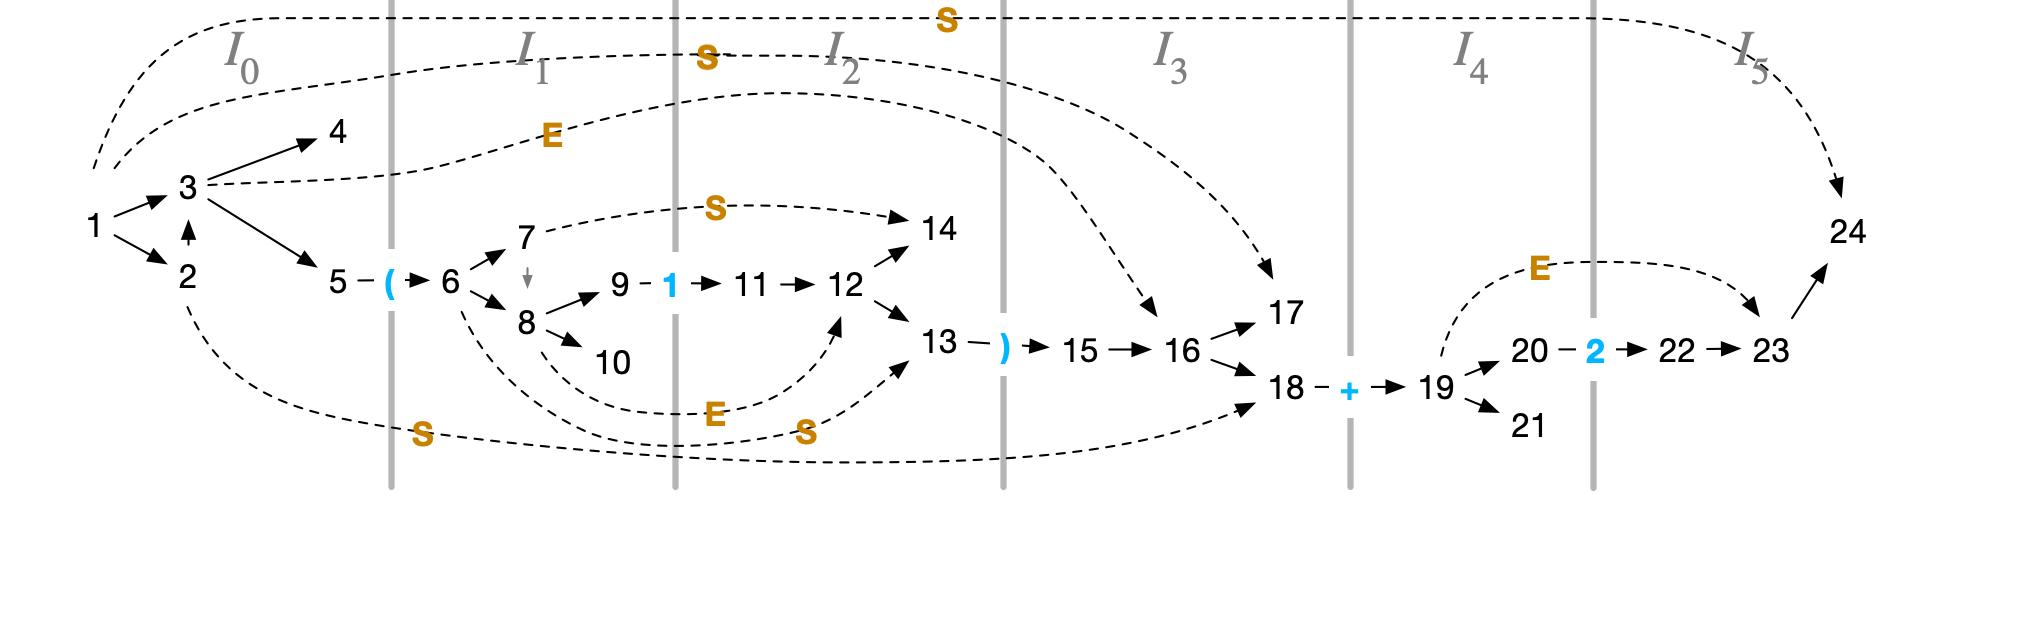
\includegraphics[scale=.4]{./chapters/earley-threads.png}
\centering
\end{figure}

Aqui, as ações de consumir tokens são anotadas com o token escaneado
em azul. As setas tracejadas mostram o estado e são rotuladas com o
não terminal que está sendo completado. Como este gráfico mostra, o
analisador explora alguns estados que não levam à análise
bem-sucedida, mas esses estados (4, 10, 14, 17 e 21) rapidamente
ficam \textbf{presos} porque não conseguem encontrar uma entrada
correspondente. Removendo esses estados e observando apenas a
sequência de produções completadas que levam ao sucesso na etapa 24,
vemos que elas descrevem uma derivação da string:

\[
\begin{array}{cccccccc}
  S' & \to & S & \to & S+E & \to & S+2 & \to \\
  24 &     & 23 &     & 18\text{--}22 &     & 16 &     \\[6pt]
  E+2 & \to & (S)+2 & \to & (E)+2 & \to & (1)+2 \\
  13\text{--}15 &     & 12 &     & 1\text{--}11 &     & \\
\end{array}
\]

Note que, a cada passo, o não terminal mais à direita é expandido
usando alguma produção. No entanto, o analisador sintático completa
essas produções de trás para frente, gerando a derivação mais à
direita invertida, começando pela entrada e terminando com o símbolo
inicial. Essa construção reversa de uma derivação mais à direita é o
que os analisadores sintáticos bottom-up fazem.

Os analisadores de Earley têm complexidade de tempo \(O(n^3)\) no
pior caso quando implementados cuidadosamente; em gramáticas não
ambíguas, a complexidade de tempo é \(O(n^2)\) no pior caso.
Intuitivamente, a razão pela qual os analisadores de Earley são
polinomiais em vez de exponenciais no pior caso é que eles
compartilham o trabalho entre as diferentes ``linhas de
processamento''. Por exemplo, observe que a conclusão única da
produção $S \to E.$ na etapa 12 realiza trabalho para duas linhas
de processamento que se ramificam na etapa 6 para os estados 7 e 8. A
linha de processamento ``7'' acaba ficando presa porque não encontra
o sinal ``+'' esperado na entrada, mas a outra linha de processamento
continua até o final.

Em gramáticas LL ou LR, os analisadores Earley são ainda mais úteis,
executando em tempo linear quando implementados cuidadosamente. Nossa
gramática de exemplo é uma gramática LR não ambígua, razão pela qual
o grafo de estados acima é predominantemente linear e pouco trabalho
é desperdiçado.

Uma otimização simples e útil é completar as produções somente quando
o token de lookahead estiver no conjunto FOLLOW do não terminal em
questão. Também pode ser útil memorizar etapas de predição em cascata.

Uma melhoria adicional que evita computação redundante é sugerida por
Aycock e Horspool
\href{https://academic.oup.com/comjnl/article-abstract/45/6/620/429185?redirectedFrom=PDF}{Practical
Earley Parsing}. Na etapa de predição, quando o símbolo C é anulável,
o item \([A\to \beta C.\gamma, k]\) é imediatamente adicionado ao
estado \(I_j\). Eles relatam que, com essa e outras otimizações, a
análise Earley é apenas 50\% mais lenta que o analisador LALR
Happy, uma compensação razoável dada a melhoria no poder de análise.

\section{Analisadores LR(0) e SLR}

A análise LR, incluindo a análise LALR, é um método popular de
análise sintática. Esses algoritmos são a tecnologia subjacente em
diversos geradores de analisadores sintáticos, como o Happy. Podemos
considerar a análise LR como uma otimização da análise Earley, na
qual todas as previsões são pré-computadas. A análise LR consiste em
duas ações: shift e reduce, portanto, os analisadores LR são chamados
de analisadores de shift-reduce. A ação de shift corresponde à ação
de consumo do algoritmo de Earley, seguida pelo máximo de previsões
possível; a ação de reduce corresponde à ação completa, novamente
seguida por previsões.

Em vez de manter o controle de todas as possíveis análises sintáticas
mais à direita, um analisador sintático de shift-reduce mantém o
controle apenas de um conjunto de análises sintáticas que
correspondem a uma única análise sintática mais à direita. Essa
limitação permite que o estado do analisador seja mais simples do que
em um analisador de Earley: o estado do analisador é baseado em uma
pilha de símbolos. Em qualquer ponto durante uma análise sintática de
shift-reduce, o estado atual da derivação é a concatenação da pilha
com a entrada não consumida. Por exemplo, podemos escrever a análise
sintática da expressão de exemplo \verb|(1)+2|
como uma série de operações de shift e reduce que constroem
exatamente a mesma derivação mais à direita que o analisador de
Earley fez acima:

\begin{table}[H]
\begin{tabular}{@{}lll@{}}
  \toprule
  Pilha de Derivação & Ações & Entrada não consumida \\
  \midrule
  (1) + 2 & (1) + 2 & \\
  (1) + 2 & shift & (1) + 2 \\
  (1) + 2 & shift & (1) + 2 \\
  (E) + 2 & reduce E $\to$ n & (E) + 2 \\
  (S) + 2 & reduce S $\to$ E & (S) + 2 \\
  (S) + 2 & shift & (S) + 2 \\
  E + 2 & reduce E $\to$ (S) & E + 2 \\
  S + 2 & reduce S $\to$ E & S + 2 \\
  S + 2 & shift & S + 2 \\
  S + 2 & shift & S + 2 \\
  S + E & reduce E $\to$ n & S + E \\
  S & reduce S $\to$ S+E & S \\
  \bottomrule
\end{tabular}
\centering
\end{table}

Para determinar qual ação deve ser tomada em cada etapa, o analisador
sintático precisa saber quais são as possíveis produções futuras a
serem reduzidas. As possíveis produções futuras são um conjunto de
itens, fechado sob predição; esse conjunto de itens nos diz qual ação
faz sentido em um determinado ponto da análise sintática. Para mapear
uma pilha em um conjunto de itens, esses conjuntos de itens podem ser
interpretados como um autômato finito determinístico que lê a pilha e
cujos estados são exatamente os conjuntos de itens. Esses estados são
semelhantes aos conjuntos de Earley, mas têm a propriedade de que,
ignorando a predição, apenas uma ação significativa pode ser tomada
em cada estado: shift ou reduce.

O estado inicial do autômato LR(0) corresponde ao conjunto de Earley
\(I_0\), exceto que adicionamos o símbolo de fim de entrada à
produção de nível superior. Assim como o conjunto de Earley, ele é
fechado sob predição.

\[
\begin{array}{l}
  S' \to . S \$\\
  S \to . S + E\\
  S \to . E\\
  E \to . n\\
  E \to . ( S )\\
\end{array}
\]

O autômato é construído repetindo-se o seguinte procedimento até que
nenhuma alteração adicional seja possível. Escolha um estado e um
símbolo que esteja à direita do ponto em uma ou mais produções.
Desloque esse símbolo para a direita nesses itens e feche o conjunto
de itens sob previsão. O conjunto de itens resultante pode ser um
estado existente do autômato ou um novo. Em ambos os casos, adicione
uma transição no símbolo escolhido do estado antigo para o estado
correspondente a este conjunto de itens.

\begin{figure}[H]
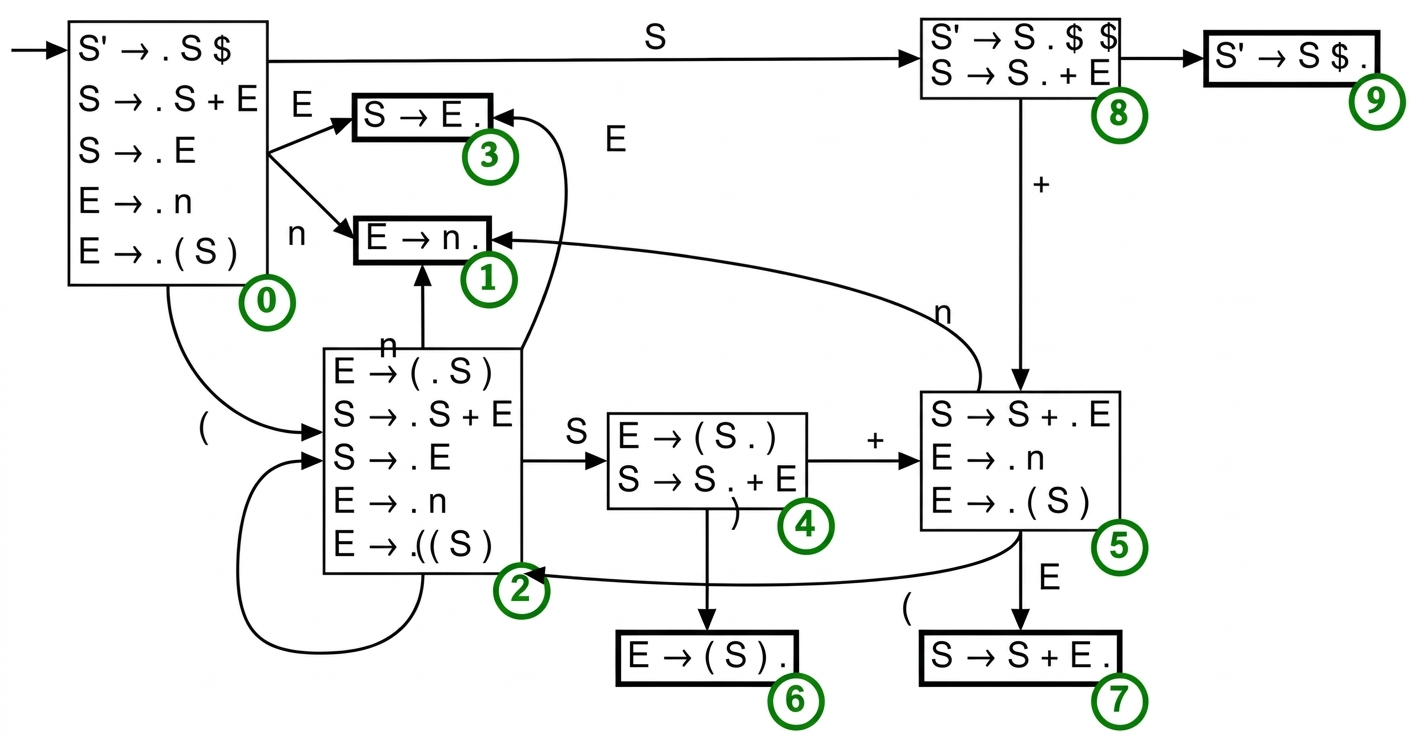
\includegraphics[scale=0.2]{./chapters/lr0.png}
\centering
\end{figure}

Por exemplo, ao realizar uma transição no token ( do estado inicial,
deslocamos apenas o último item para a direita, obtendo um estado
contendo a produção \(E \to ( . S )\), sobre o qual então realizamos
um fechamento de predição que adiciona itens para \(S\) e, em
seguida, para \(E\). Ao realizar uma transição a partir do mesmo
estado no não terminal S, deslocamos os dois primeiros itens para a
direita, obtendo os itens $S' \to S . \$$ e \(S \to S.+E\). O
fechamento de predição não adiciona nenhum item a este estado. A
figura a seguir mostra os passos que você pode seguir para completar
o autômato (pressione o botão para avançar a animação). Na figura, os
estados estão numerados em verde e os estados nos quais uma ação de
redução deve ser realizada têm uma borda mais espessa.

Podemos resumir este autômato em duas tabelas que podem ser usadas
para controlar um analisador sintático. A primeira é a tabela action,
que informa ao analisador o que fazer em cada estado, dado o símbolo
de previsão: shift e ir para um novo estado, ou reduce por alguma
produção. A segunda tabela é a tabela goto, que informa ao analisador
para qual estado ir quando ele reduz uma produção. Abaixo estão essas
duas tabelas do autômato que acabamos de construir, lado a lado.
Entradas vazias nas tabelas correspondem a erros de sintaxe. Entradas
numéricas na tabela action correspondem a ações de shift; uma
produção na tabela action indica uma ação de reduce.

\begin{table}[H]
  \begin{tabular}{@{}llllllll@{}}
    \toprule
    & n & + & ( & ) & \$ & S & E \\
    \midrule
    0 & 1 & & 2 & & & 8 & 3 \\
    1 & E $\to$ n & E $\to$ n & E $\to$ n & E $\to$ n & E $\to$ n & & \\
    2 & 1 & & 2 & & & 4 & 3 \\
    3 & S $\to$ E & S $\to$ E & S $\to$ E & S $\to$ E & S $\to$ E & & \\
    4 & & 5 & & 6 & & & \\
    5 & 1 & & 2 & & & & 7 \\
    6 & E $\to$ (S) & E $\to$ (S) & E $\to$ (S) & E $\to$ (S) & E
    $\to$ (S) & & \\
    7 & S $\to$ S+E & S $\to$ S+E & S $\to$ S+E & S $\to$ S+E & S
    $\to$ S+E & & \\
    8 & & 5 & & & 9 & & \\
    9 & \(S'\to S\). & \(S' \to S\). & \(S'\to S\). & \(S' \to S\). & \(S'\to
    S\$\). & & \\
    \bottomrule
  \end{tabular}
  \centering
\end{table}

Durante sua execução, um analisador sintático shift-reduce utiliza
uma tabela (como a apresentada) e uma pilha de estados. O algoritmo
inicia com a pilha contendo o estado inicial e a entrada a ser
processada. À medida que lê cada token de entrada, ele consulta na
tabela action qual é a ação atual para o estado no topo da pilha,
dado o próximo token. Se a ação for um shift, ele adiciona o estado
especificado à pilha. Se a ação for um reduce, ele remove da pilha o
número de itens na produção correspondente e usa a tabela goto do
estado agora no topo da pilha para determinar o próximo estado a ser
adicionado à pilha.

Vamos testar este analisador sintático no exemplo anterior,
\verb|(1)+2|. A pilha contém apenas o estado 0.
Para tornar mais claro, os estados na pilha são mostrados em
\textbf{negrito} e são precedidos pelo símbolo que foi seguido para
chegar a esse estado. Esses símbolos correspondem à parte da
derivação que foi construída até agora pelo analisador sintático.
\begin{table}[H]
  \begin{tabular}{@{}lll@{}}
    \toprule
    Pilha & Entrada & Ação \\
    \midrule
    \textbf{0} & (1)+2 & shift \textbf{2} \\
    \textbf{0}(\textbf{2} & 1)+2 & shift \textbf{1} \\
    \textbf{0}(\textbf{21} & )+2 & reduce E $\to$ n \\
    \textbf{0}(\textbf{2}E\textbf{3} & )+2 & reduce S $\to$ E \\
    \textbf{0}(\textbf{2}S\textbf{4} & )+2 & shift \textbf{6} \\
    \textbf{0}(\textbf{2}S\textbf{4})\textbf{6} & +2 & reduce E $\to$ (S) \\
    \textbf{0}E\textbf{3} & +2 & reduce S $\to$ E \\
    \textbf{0}S\textbf{8} & +2 & shift \textbf{5} \\
    \textbf{0}S\textbf{8}+\textbf{5} & 2 & shift \textbf{1} \\
    \textbf{0}S\textbf{8}+\textbf{51} & \$ & reduce E $\to$ n \\
    \textbf{0}S\textbf{8}+\textbf{5}E\textbf{7} & \$ & reduce S $\to$ S+E \\
    \textbf{0}S\textbf{8} & \$ & shift \textbf{9} \\
    \textbf{0}S\textbf{8}\$\textbf{9} & & reduce S' $\to$ S \\
    \bottomrule
  \end{tabular}
  \centering
\end{table}

Note que a construção LR que vimos até agora não faz nada além de
reduzir a uma única produção fixa, independentemente do próximo token
na entrada. Como resultado, os estados que contêm reduções (estados
1, 3, 6, 7, 9 no exemplo) ignoram o token de lookahead. A esse
algoritmo damos o nome de analisador LR(0). Preenchendo as tabelas de
action e goto de uma maneira menos restritiva, poderíamos obter um
analisador LR(1), que é mais expressivo. No entanto, precisaremos
modificar a construção da tabela LR(0) que acabamos de ver para obter
essa expressividade.

Uma extensão simples, mas surpreendentemente eficaz, para LR(0) é
adicionar uma ação de redução à tabela de ações apenas no caso em que
o token de lookahead esteja no conjunto FOLLOW do não terminal que
está sendo reduzido, já que, caso contrário, a produção claramente
não leva a uma análise válida. Quando esse refinamento na construção
LR(0) produz um analisador sintático shift-reduce válido, dizemos que
a gramática é SLR (Simple LR).

\section{Implementação}

Nesta seção comentamos os principais detalhes das implementações
Haskell dos algoritmos apresentados neste capítulo.

\subsection{Algoritmo de Earley}

A implementação está no módulo
\verb|Parsing.Earley.EarleyParser|. Os tipos
principais refletem diretamente as definições do algoritmo apresentadas acima.

\subsubsection{Itens e conjuntos}

Um item Earley \([A \to \beta . \gamma, k]\) é representado pelo tipo:

\begin{minted}{haskell}
data EarleyItem = EarleyItem
  { itemLhs :: String    -- não-terminal do lado esquerdo
  , itemBefore :: [Symbol]  -- símbolos antes do ponto
  , itemAfter :: [Symbol]  -- símbolos depois do ponto
  , itemOrigin :: Int -- posição de início
  }
\end{minted}

O campo \haskell{itemOrigin} corresponde ao índice
\(k\) do item \([A \to \beta.\gamma, k]\): ele registra em qual
conjunto Earley este item se originou, o que é usado na etapa de
completar. O chart completo é uma lista de conjuntos:

\begin{minted}{haskell}
type EarleySet = [EarleyItem]
type Chart = [EarleySet]
\end{minted}

O chart tem \(n + 1\) conjuntos, \(I_0\) a \(I_n\), onde \(n\) é o
comprimento da entrada.

\subsubsection{As três operações}

As três operações do algoritmo são funções puras:

\begin{minted}{haskell}
-- predição
predictItems :: Grammar -> Int -> EarleyItem -> [EarleyItem]
-- verificação
scanItems :: String -> EarleySet -> [EarleyItem]
-- completar
completeItems :: Chart -> EarleySet -> Int -> EarleyItem -> [EarleyItem]
\end{minted}

A função \haskell{completeItems} precisa de acesso ao
chart anterior para buscar os itens que esperavam o não-terminal
\(B\) completado. Quando o item completado tem
\haskell{itemOrigin = j < k}, a busca é feita em
\haskell{"chart !! j"} (já fechado); quando
\haskell{j = k}, busca-se em
\haskell{currentSet}, o conjunto sendo construído,
para lidar com completações em cadeia no mesmo conjunto.

\subsubsection{Fechamento de um conjunto}

A função \haskell{closeSet} aplica predição e
completar repetidamente usando um algoritmo de worklist: novos itens
gerados vão para o final da fila e são processados em ordem, evitando
elementos duplicados:

\begin{minted}{haskell}
closeSet :: Grammar -> Chart -> Int -> [EarleyItem] -> EarleySet
closeSet grammar prevSets k = go []
  where
    go current []           = current
    go current (item : rest)
      | item `elem` current = go current rest
      | otherwise =
          let current' = current ++ [item]
              new      = predictItems grammar k item
                      ++ completeItems prevSets current' k item
          in go current' (rest ++ new)
\end{minted}

Esta estrutura garante que cada item seja processado apenas uma vez,
assim como o algoritmo descrito na seção anterior assegura que as
três regras são aplicadas ``quantas vezes forem necessárias até que
nenhuma delas tenha efeito''.

\subsubsection{Construção do chart e aceitação}

A função \haskell{buildChart} constrói \(I_0\)
fechando os itens iniciais do símbolo de partida, depois aplica
\haskell{scanItems} para obter o conjunto inicial de
cada \(I_{k+1}\) e fecha-o:

\begin{minted}{haskell}
buildChart :: Grammar -> [String] -> Chart
buildChart grammar tokens = go [s0] tokens
  where
    s0 = closeSet grammar [] 0 startItems
    go chart []           = chart
    go chart (tok : toks) =
        let sk1 = closeSet grammar chart (length chart) (scanItems tok (last chart))
        in go (chart ++ [sk1]) toks
\end{minted}

A entrada é aceita se \(I_n\) contém um item completo para o símbolo
inicial com origem em 0, exatamente a condição \([S' \to S., 0]
\in I_n\) descrita na introdução do algoritmo:

\begin{minted}{haskell}
earleyParse :: Grammar -> [String] -> EarleyResult
earleyParse grammar tokens
    | any accept (chart !! n) = EarleyAccept
    | otherwise               = EarleyReject
  where
    n     = length tokens
    chart = buildChart grammar tokens
    accept item = itemLhs item == start && itemOrigin item == 0
               && null (itemAfter item)
\end{minted}

\subsection{LR(0) e SLR}

A implementação está distribuída em três módulos:
\begin{flushleft}
  \verb|Parsing.LR.LR0.BuildTable|,\\
  \verb|Parsing.LR.LR0.LR0Parser| e\\
  \verb|Parsing.LR.SLR.BuildTable|.
\end{flushleft}

\subsubsection{Itens e estados LR(0)}

Um item LR(0) \(A \to \alpha . \beta\) é mais simples que um item
Earley: não carrega a posição de origem, pois os estados do autômato
já capturam essa informação implicitamente:

\begin{minted}{haskell}
data Item = Item
  { itemLHS :: String    -- não-terminal
  , itemBefore :: [Symbol]  -- símbolos antes do ponto
  , itemAfter :: [Symbol]  -- símbolos depois do ponto
  }

type State = Set Item
\end{minted}

Um estado LR(0) é um conjunto de itens, exatamente como os conjuntos
de itens apresentados na seção anterior. O autômato cujos estados são
esses conjuntos é o DFA que lê a pilha do analisador.

\subsubsection{Fechamento e transições}

A função \haskell{closure} implementa o fechamento de
predição descrito no capítulo: para cada item com um não-terminal
\(C\) após o ponto, adiciona todos os itens \(C \to . \gamma\):

\begin{minted}{haskell}
closure :: Grammar -> State -> State
closure g = fixedPoint step
  where
    step current = Set.union current $ Set.fromList
        [ Item b [] prod
        | item <- Set.toList current
        , NonTerminal b <- take 1 (itemAfter item)
        , prod <- fromMaybe [] (Map.lookup b g)
        ]
\end{minted}

A função \haskell{goto} computa a transição do
autômato ao consumir um símbolo: avança o ponto nos itens que têm
esse símbolo imediatamente após ele e fecha o resultado:

\begin{minted}{haskell}
goto :: Grammar -> State -> Symbol -> State
goto g items sym = closure g $ Set.fromList
    [ Item lhs (before ++ [sym]) rest
    | Item lhs before (s:rest) <- Set.toList items
    , s == sym
    ]
\end{minted}

A função \haskell{buildStates} constrói a coleção
canônica de estados LR(0) por busca em largura, partindo do estado
inicial que contém o item \(S' \to . S\) da gramática aumentada:

\begin{minted}{haskell}
buildStates :: Grammar -> [State]
buildStates g = buildFrom [initial] [initial]
  where
    initial = closure g' (Set.singleton $ initialItem g')
    buildFrom seen [] = seen
    buildFrom seen (cur : queue) =
        let newStates = [goto g' cur sym | sym <- nextSymbols cur]
            unseen    = filter (`notElem` seen) newStates
        in buildFrom (seen ++ unseen) (queue ++ unseen)
\end{minted}

\subsubsection{Tabela de parsing LR(0)}

A tabela de parsing tem duas partes: a tabela
\haskell{action}, que mapeia
\haskell{(estado, terminal)} para uma ação, e a
tabela \haskell{goto}, que mapeia
\haskell{(estado, não-terminal)} para o próximo
estado após uma redução:

\begin{minted}{haskell}
data Action = Shift Int | Reduce String [Symbol] | Accept

data ParsingTable = ParsingTable
  { actionTable :: Map (Int, String) Action
  , gotoTable :: Map (Int, String) Int
  , states :: [State]
  }
\end{minted}

O preenchimento da tabela segue as regras descritas na seção de LR(0):

\begin{itemize}
  \item
    \textbf{Shift}: para cada terminal \(t\) após o ponto em algum
    item de um estado \(i\), action[i, t] = Shift j, onde
    \(j\) é o índice do estado
    \haskell{goto(i, t)}.
  \item
    \textbf{Reduce (LR(0))}: para cada item completo \(A \to \alpha
    .\) em um estado \(i\), action[i, t] =
    Reduce($A \to \alpha$) para \textbf{todos} os terminais \(t\) da
    gramática. Esta é a característica do LR(0): ele ignora o
    lookahead nas reduções.
  \item
    \textbf{Accept}: quando o item completo é \(S' \to S .\),
    action[i, \$] = Accept.
\end{itemize}

\subsubsection{O algoritmo de parsing LR(0)}

O algoritmo de parsing mantém uma pilha de estados e processa a
entrada símbolo a símbolo. O tipo
\haskell{ParserState} encapsula o estado completo do analisador:

\begin{minted}{haskell}
data ParserState = ParserState
  { stateStack :: [Int] -- pilha de estados
  , symbolStack :: [Symbol]  -- pilha de símbolos (para diagnóstico)
  , inputBuffer :: [String]  -- entrada restante
  }
\end{minted}

A função \haskell{parseStep} executa um único passo:
consulta action[estado\_topo, token] e
aplica a ação correspondente:

\begin{itemize}
  \item
    \textbf{Shift n}: empilha o estado \haskell{n} e
    avança na entrada.
  \item
    \textbf{Reduce $A \to \alpha$}: desempilha $\alpha$
    estados e empilha o estado dado por
    goto[novo\_topo, A]. Depois chama
    \haskell{parseStep} recursivamente pois a entrada
    não é consumida em reduções.
  \item
    \textbf{Accept}: sinaliza sucesso.
\end{itemize}

\begin{minted}{haskell}
parseLR0 :: Grammar -> ParsingTable -> [String] -> ParseResult
parseLR0 g table tokens = go (ParserState [0] [] (tokens ++ ["$"]))
\end{minted}

\subsubsection{A diferença do SLR}

O módulo \verb|Parsing.LR.SLR.BuildTable|
reutiliza toda a infraestrutura de LR(0):
\haskell{buildStates},
\haskell{closure}, \haskell{goto},
\haskell{parseLR0}. A implementação do SLR modifica apenas a geração
das entradas de redução. Enquanto LR(0) adiciona Reduce para todos os
terminais, SLR restringe às entradas cujo terminal pertence a
\(\mathrm{FOLLOW}(A)\):

\begin{minted}{haskell}
-- LR(0): reduz em todos os terminais
reduceA = [ ((i, t), Reduce lhs alpha)
          | item <- Set.toList state, null (itemAfter item)
          , t <- terminals g ++ ["$"] ]

-- SLR: reduz apenas nos terminais em FOLLOW(lhs)
reduceA = [ ((i, t), Reduce lhs alpha)
          | item <- Set.toList state, null (itemAfter item)
          , t <- fromMaybe [] (Map.lookup lhs followSets) ]
\end{minted}

Esta mudança pontual é suficiente para que a gramática de expressões
\[
  \begin{array}{lcl}
    E & \to  & E + T \\
    & \mid & T \\
    T & \to  & T * F \\
    & \mid & F \\
    F & \to  & (E) \\
    & \mid & n
  \end{array}
\]
deixe de ter conflitos: no estado que contém \(E \to T.\) e \(T
\to T.*F\), LR(0) colocaria Reduce \(E \to T\) em
$*$, gerando um conflito com Shift. Com SLR,
como \(* \notin \mathrm{FOLLOW}(E) = \{+, ), \$\}\), a entrada
action[estado, *] recebe apenas Shift, não resultando em conflito.

\section{Conclusão}

Este capítulo explorou técnicas bottom-up para análise sintática,
destacando como estas oferecem maior expressividade ao lidar com
recursão à esquerda e prefixos mais longos da entrada. Investigamos o
Algoritmo de Earley, uma solução robusta capaz de processar qualquer
gramática livre de contexto através da simulação de múltiplas frentes
de análise em paralelo, e introduzimos os fundamentos da análise
LR(0) e SLR, que otimizam esse processo via autômatos de shift-reduce
e pilhas de estados. Embora o SLR melhore a eficiência ao utilizar
conjuntos FOLLOW para decidir reduções, ele ainda apresenta
limitações em gramáticas mais complexas. Para superar essas
restrições, o próximo capítulo abordará os algoritmos LR(1) e LALR.

\chapter{Análise sintática LR(1) e LALR}

\section{Introdução}\label{introduuxe7uxe3o}

No capítulo anterior, vimos os algoritmos LR(0) e SLR. O LR(0)
constrói um autômato cujos estados são conjuntos de itens da forma
\(A \to \beta . \gamma\) e preenche a tabela de ações sem considerar
o próximo token de entrada: toda entrada de reduce é preenchida para
\textbf{todos} os terminais.

Para motivar a necessidade de ir além do LR(0), considere a seguinte
gramática de expressões com recursão à \textbf{esquerda}:

\[
  \begin{array}{lcl}
    E & \to & E + T \mid T \\
    T & \to & n \mid ( E )
  \end{array}
\]

Essa gramática é LR(0): nenhum estado do autômato possui
simultaneamente um item completo e um item não completo com o mesmo
símbolo à direita do ponto. Por exemplo, o estado obtido após
reconhecer \(E\) no estado inicial contém:

\[
  \begin{array}{l}
    S' \to E . \\
    E \to E . + T
  \end{array}
\]

O primeiro item é aceitar em \(\$\) e o segundo é um shift em \(+\),
portanto não há conflito.

Agora modifiquemos a gramática para usar recursão à \textbf{direita}:

\[
  \begin{array}{lcl}
    E & \to & T + E \mid T \\
    T & \to & n \mid ( E )
  \end{array}
\]

Com essa mudança, o estado obtido após reconhecer \(T\) no estado
inicial passa a conter:

\[
  \begin{array}{l}
    E \to T . + E \\
    E \to T .
  \end{array}
\]

O item \(E \to T.\) está completo, então a construção LR(0) insere
uma ação de reduce \(E \to T\) para \textbf{todos} os terminais,
incluindo \(+\). Mas \(E \to T . + E\) exige uma ação de shift em
\(+\). Temos, portanto, um \textbf{conflito shift-reduce} em \(+\)
que o LR(0) não consegue resolver.

A raiz do problema é clara: quando o próximo token é \(+\), ainda é
possível completar \(E \to T + E\), portanto \textbf{não} devemos
reduzir. Quando o próximo token é \(\$\) ou \()\), não há como
continuar e \textbf{devemos} reduzir. Basta um único token de
lookahead para tomar a decisão correta.

Isso nos leva ao algoritmo \textbf{LR(1)}, que inclui em cada item
com um conjunto de lookaheads calculados localmente, não
globalmente como o SLR, tornando as ações de reduce precisas o
suficiente para resolver esses conflitos. O algoritmo
\textbf{LALR(1)} é uma variante prática do LR(1) que mantém o mesmo
número de estados do LR(0) ao fundir estados com o mesmo núcleo,
reunindo seus lookaheads.

\section{O Algoritmo LR(1)}

O algoritmo LR(1) constrói um autômato cujos estados representam o
progresso simultâneo de todas as derivações possíveis no contexto
atual. A cada estado está associado um conjunto de \textbf{itens
LR(1)}, cada um descrevendo o quanto de uma produção já foi analisado
e qual token pode legitimamente aparecer a seguir caso essa produção
seja completada. A partir desses estados, são extraídas as tabelas de
ações (shift, reduce, accept) e goto que guiam o analisador.

\subsection{Itens LR(1)}

Um \textbf{item LR(1)} tem a forma \([A \to \beta . \gamma, a]\). A
produção \(A \to \beta \gamma\) indica qual regra está sendo
reconhecida; o ponto separa a parte \(\beta\) já processada, que está
no topo da pilha, da parte \(\gamma\) que ainda está por vir na
entrada. O componente \(\alpha\) é o \textbf{lookahead}: um terminal (ou
\(\$\)) que pode aparecer imediatamente depois de toda a cadeia
derivada de \(A\) no contexto em que este item foi gerado. Ao
contrário do SLR, que calcula lookaheads globalmente usando conjuntos
FOLLOW, o LR(1) os deriva localmente a partir do contexto de cada item.

Quando o item está completo; isto é, quando \(\gamma =
\lambda\); o lookahead determina exatamente em qual coluna da
tabela de ações a redução \(A \to \beta\) deve ser inserida, evitando
conflitos com ações de shift que porventura também estejam presentes
no mesmo estado.

\subsection{Fechamento LR(1)}

O fechamento de um conjunto de itens LR(1) propaga as previsões de
forma análoga ao LR(0), mas agora carregando o lookahead correto para
cada nova previsão. Dado um item \([A \to \alpha . B \beta, a]\) em
que o próximo símbolo após o ponto é o não-terminal \(B\), para cada
produção \(B \to \gamma\) da gramática adicionamos ao conjunto o item
\([B \to . \gamma, b]\), onde \(b\) percorre todos os elementos de
\(\text{FIRST}(\beta\, a)\). Esse conjunto capta exatamente os
terminais que podem aparecer depois de \(B\) neste contexto: se
\(\beta\) não for anulável, são os primeiros de \(\beta\); se
\(\beta\) for anulável ou vazio, o próprio lookahead \(a\) também é
incluído. O processo é repetido até que nenhum item novo seja adicionado.

\subsection{Função goto LR(1)}

A transição entre estados é calculada pela função \(\text{goto}(I,
X)\), que recebe um estado \(I\) e um símbolo \(X\) (terminal ou
não-terminal) e devolve o estado alcançado após reconhecer \(X\).
Para construí-lo, tomamos todos os itens de \(I\) que têm \(X\)
imediatamente após o ponto, isto é, itens da forma \([A \to \alpha . X
\beta, a]\), avançamos o ponto para obter \([A \to \alpha X .
\beta, a]\) e calculamos o fechamento desse conjunto. O lookahead
\(a\) é transferido sem alteração, pois ele depende do contexto em
que o item foi criado, não do símbolo recém-reconhecido.

\subsection{Construção da Tabela LR(1)}

A construção começa com o estado inicial \(I_0\), obtido pelo
fechamento do item-semente \([S' \to . S, \$]\), onde \(S'\) é o
símbolo de partida aumentado. A partir de \(I_0\), novos estados são
gerados aplicando-se \(\text{goto}\) para cada símbolo que aparece à
direita de algum ponto no estado atual; esse processo é repetido para
todos os estados descobertos até que não haja mais novidades.

Com os estados em mãos, a tabela de ações é preenchida da seguinte
forma. Para cada item \([A \to \alpha . a \beta, b]\) em que \(a\) é
um terminal, insere-se um shift para o estado \(\text{goto}(I, a)\)
na entrada \(\text{action}[I, a]\). Para cada item completo \([A \to
\alpha ., a]\) com \(A \neq S'\), insere-se uma redução \(A \to
\alpha\) na entrada \(\text{action}[I, a]\): apenas na coluna do
lookahead \(a\), não em todas. Finalmente, quando o item \([S' \to S
., \$]\) está presente, registra-se accept em \(\text{action}[I,
\$]\). A tabela goto é preenchida com \(\text{goto}[I, B] =
\text{goto}(I, B)\) para cada não-terminal \(B\). Se nenhum par \((I,
a)\) receber duas ações distintas, a gramática é \textbf{LR(1)}.

\section{Exemplo: Tabela LR(1) para Expressões Aritméticas}

Considere a gramática de expressões com precedência:

\[
\begin{array}{lcl}
  E & \to & E + T \mid T \\
  T & \to & T \star F \mid F \\
  F & \to & ( E ) \mid n
\end{array}
\]

Aumentamos a gramática com \(S' \to E\).

\subsection{Construção dos estados}

\textbf{Estado 0}: fechamento de \(\{[S' \to . E, \$]\}\):

\[
\begin{array}{ll}
  S' \to . E    & \$ \\
  E \to . E + T & \$,+ \\
  E \to . T     & \$,+ \\
  T \to . T \star F & \$,+,\star \\
  T \to . F     & \$,+,\star \\
F \to . ( E ) & \$,+,\star,) \\
F \to . n     & \$,+,\star,)\\
\end{array}
\]

\textbf{Estado 1}: \(\text{goto}(I_0, E)\):

\[
\begin{array}{ll}
S' \to E . & \$ \\
E \to E . + T & \$,+
\end{array}
\]

\textbf{Estado 2}: \(\text{goto}(I_0, T)\):

\[
\begin{array}{ll}
E \to T . & \$,+ \\
T \to T . \star F & \$,+,\star
\end{array}
\]

\textbf{Estado 3}: \(\text{goto}(I_0, F)\):

\[
\begin{array}{ll}
T \to F . & \$,+,\star
\end{array}
\]

\textbf{Estado 4}: \(\text{goto}(I_0, ()\):

\[
\begin{array}{ll}
F \to ( . E ) & \$,+,\star,) \\
E \to . E + T & ),+ \\
E \to . T & ),+ \\
T \to . T * F & ),+,\star \\
T \to . F & ),+,\star \\
F \to . ( E ) & ),+,\star,( \\
F \to . n & ),+,\star,(
\end{array}
\]

\textbf{Estado 5}: \(\text{goto}(I_0, n)\):

\[
\begin{array}{ll}
F \to n . & \$,+,\star,)
\end{array}
\]

\textbf{Estado 6}: \(\text{goto}(I_1, +)\):

\[
\begin{array}{ll}
E \to E + . T & \$,+ \\
T \to . T * F & \$,+,\star \\
T \to . F & \$,+,\star \\
F \to . ( E ) & \$,+,\star,) \\
F \to . n & \$,+,\star,)
\end{array}
\]

\textbf{Estado 7}: \(\text{goto}(I_2, \star)\):

\[
\begin{array}{ll}
T \to T \star . F & \$,+,\star \\
F \to . ( E ) & \$,+,\star,) \\
F \to . n & \$,+,\star,)
\end{array}
\]

\textbf{Estado 8}: \(\text{goto}(I_4, E)\):

\[
\begin{array}{ll}
F \to ( E . ) & \$,+,\star,) \\
E \to E . + T & ),+
\end{array}
\]

\textbf{Estado 9}: \(\text{goto}(I_4, T)\):

\[
\begin{array}{ll}
E \to T . & ),+ \\
T \to T . \star F & ),+,\star
\end{array}
\]

\textbf{Estado 10}: \(\text{goto}(I_4, F)\) = \(\text{goto}(I_6,
F)\) = \(\text{goto}(I_7, F)\):

\[
\begin{array}{ll}
T \to F . & \$,+,\star,)
\end{array}
\]

(Estados 10--12 para os retornos dos subestados de 4 e 6 são
análogos; por simplicidade, listamos apenas os mais relevantes.)

\textbf{Estado 11}: \(\text{goto}(I_6, T)\):

\[
\begin{array}{ll}
E \to E + T . & \$,+ \\
T \to T . \star F & \$,+,\star
\end{array}
\]

\textbf{Estado 12}: \(\text{goto}(I_7, F)\):

\[
\begin{array}{ll}
T \to T \star F . & \$,+,\star,)
\end{array}
\]

\textbf{Estado 13}: \(\text{goto}(I_8, ))\):

\[
\begin{array}{ll}
F \to ( E ) . & \$,+,\star,)
\end{array}
\]

\textbf{Estado 14}: \(\text{goto}(I_8, +)\):

\[
\begin{array}{ll}
E \to E + . T & ),+ \\
T \to . T \star F & ),+,\star \\
T \to . F & ),+,\star \\
F \to . ( E ) & ),+,\star,( \\
F \to . n & ),+,\star,(
\end{array}
\]

\textbf{Estado 15}: \(\text{goto}(I_9, \star)\):

\[
\begin{array}{ll}
T \to T \star . F & ),+,\star \\
F \to . ( E ) & ),+,\star,( \\
F \to . n & ),+,\star,(
\end{array}
\]

\subsection{Tabela LR(1)}\label{tabela-lr1}

Os estados com itens completos têm reduções restritas aos lookaheads do item:

\begin{table}[H]
\begin{tabular}{@{}llllllllll@{}}
\toprule
Estado & n & + & $\star$ & ( & ) & \$ & E & T & F \\
\midrule
0 & s5 & & & s4 & & & 1 & 2 & 3 \\
1 & & s6 & & & & acc & & & \\
2 & & r E→T & s7 & & & r E→T & & & \\
3 & & r T→F & r T→F & & & r T→F & & & \\
4 & s5 & & & s4 & & & 8 & 9 & 3 \\
5 & & r F→n & r F→n & & r F→n & r F→n & & & \\
6 & s5 & & & s4 & & & & 11 & 10 \\
7 & s5 & & & s4 & & & & & 12 \\
8 & & s14 & & & s13 & & & & \\
9 & & r E→T & s15 & & r E→T & & & & \\
10 & & r T→F & r T→F & & r T→F & r T→F & & & \\
11 & & r E→E+T & s7 & & & r E→E+T & & & \\
12 & & r T→T*F & r T→T*F & & & r T→T*F & & & \\
13 & & r F→(E) & r F→(E) & & r F→(E) & r F→(E) & & & \\
14 & s5 & & & s4 & & & & 16 & 10 \\
15 & s5 & & & s4 & & & & & 17 \\
\bottomrule
\end{tabular}
\centering
\end{table}

(Estados 16 e 17 são análogos a 11 e 12, mas com lookaheads \(\{),+\}\).)

Observe que cada ação de reduce aparece apenas nas colunas
correspondentes ao lookahead do item, não em todas as colunas como no
LR(0). Isso evita conflitos que o SLR não conseguiria resolver quando
o conjunto FOLLOW é impreciso.

\section{O Algoritmo LALR(1)}

O LALR(1) (Look-Ahead LR) é uma simplificação prática do LR(1) que
reduz o número de estados sem abrir mão dos lookaheads locais. A
ideia central é observar que vários estados LR(1) distintos
compartilham o mesmo \textbf{núcleo}; isto é, os mesmos itens
quando ignoramos os lookaheads; e podem ser fundidos em um único
estado sem comprometer a correção do analisador na maioria das
gramáticas de interesse prático.

\subsection{Motivação}

O LR(1) resolve conflitos ao custo de multiplicar estados: dois
contextos diferentes que levam ao mesmo conjunto de itens LR(0) geram
estados LR(1) distintos porque seus lookaheads diferem. Na gramática
de expressões acima, por exemplo, os estados 3 e 10 têm o mesmo
núcleo \(T \to F .\), mas lookaheads diferentes: o estado 3,
originado fora de parênteses, carrega \(\{\$, +, \star\}\), enquanto
o estado 10, originado dentro de parênteses, carrega \(\{\$, +,
\star, )\}\). Para gramáticas de linguagens de programação realistas,
essa duplicação pode fazer o número de estados LR(1) ser uma ordem de
grandeza maior do que o número de estados LR(0), tornando as tabelas
proibitivamente grandes.

\subsection{Fusão de Estados}

O LALR(1) contorna esse problema fundindo todos os estados LR(1) que
compartilham o mesmo núcleo. O estado resultante reúne os lookaheads
de todos os estados fundidos, tomando a união dos conjuntos. Todas as
transições que apontavam para qualquer um dos estados originais
passam a apontar para o estado fundido. Como o núcleo (e portanto
a estrutura de shift e goto) é idêntico em todos os estados
mesclados, as transições permanecem consistentes após a fusão.

O único risco introduzido pela fusão é o surgimento de conflitos
reduce-reduce: se dois itens completos com o mesmo núcleo tinham
lookaheads disjuntos antes da fusão, sua união pode fazer com que
ambos reivindiquem a mesma entrada na tabela de ações. Quando isso
ocorre, a gramática é LR(1) mas não LALR(1). Vale notar que conflitos
shift-reduce nunca são introduzidos pela fusão: um shift é
determinado pelo núcleo do item, não pelo lookahead, de modo que um
conflito desse tipo no estado fundido já existiria nos estados LR(1) originais.

\subsection{Construção da Tabela LALR(1)}

Na prática, a tabela LALR(1) é obtida calculando-se primeiro todos os
estados LR(1), agrupando os que têm o mesmo núcleo e unindo seus
lookaheads. A tabela de ações e goto é então preenchida sobre os
estados fundidos exatamente da mesma forma que no LR(1): shifts são
determinados pelo núcleo do item, reduces são restritos ao lookahead
do item completo e accept ocorre ao atingir o item \([S' \to S .,
\$]\). O resultado é um analisador com o mesmo número de estados do
LR(0) e lookaheads mais precisos que o SLR.

\section{Exemplo: Tabela LALR(1) para Expressões Aritméticas}

Retomamos a mesma gramática de expressões do exemplo anterior.

\subsection{Identificação de estados com o mesmo núcleo}

Comparando os estados LR(1) construídos acima, identificamos os
seguintes grupos com o mesmo núcleo:

\begin{table}[H]
\begin{tabular}{@{}lll@{}}
\toprule
Núcleo & Estados LR(1) & Lookaheads unidos \\
\midrule
$T \to F .$ & 3 e 10 & $\{\$,+,\star,)\}$ \\
$E \to E + . T$, $T \to . T \star F$, $T \to . F$, \ldots & 6 e 14 &
$\{\$,+,)\}$ \\
$T \to T \star . F$, $F \to . (E)$, $F \to . n$ & 7 e 15 & $\{\$,+,\star,)\}$ \\
$E \to E + T .$, $T \to T . \star F$ & 11 e 16 & $\{\$,+,)\}$ \\
$T \to T \star F .$ & 12 e 17 & $\{\$,+,\star,)\}$ \\
\bottomrule
\end{tabular}
\centering
\end{table}

Os demais estados (0, 1, 2, 4, 5, 8, 9, 13) têm núcleos únicos e não
são fundidos.

Após a fusão, os estados LALR são nomeados como: \textbf{0, 1, 2,
3+10, 4, 5, 6+14, 7+15, 8, 9, 11+16, 12+17, 13}.

\subsection{Estados LALR resultantes}

\textbf{Estado 3+10} (fusão de 3 e 10):

\[
\begin{array}{ll}
T \to F . & \$,+,\star,)
\end{array}
\]

\textbf{Estado 6+14} (fusão de 6 e 14):

\[
\begin{array}{ll}
E \to E + . T & \$,+,) \\
T \to . T \star F & \$,+,\star,) \\
T \to . F & \$,+,\star,) \\
F \to . ( E ) & \$,+,\star,),( \\
F \to . n & \$,+,\star,),(
\end{array}
\]

\textbf{Estado 7+15} (fusão de 7 e 15):

\[
\begin{array}{ll}
T \to T \star . F & \$,+,\star,) \\
F \to . ( E ) & \$,+,\star,),( \\
F \to . n & \$,+,\star,),(
\end{array}
\]

\textbf{Estado 11+16} (fusão de 11 e 16):

\[
\begin{array}{ll}
E \to E + T . & \$,+,) \\
T \to T . \star F & \$,+,\star,)
\end{array}
\]

\textbf{Estado 12+17} (fusão de 12 e 17):

\[
\begin{array}{ll}
T \to T \star F . & \$,+,\star,)
\end{array}
\]

\subsection{Tabela LALR(1)}

A tabela LALR é construída sobre os estados fundidos. Usamos nomes
curtos para os estados fundidos: \textbf{A} = 3+10, \textbf{B} =
6+14, \textbf{C} = 7+15, \textbf{D} = 11+16, \textbf{E} = 12+17.

\begin{table}[H]
\begin{tabular}{@{}llllllllll@{}}
\toprule
Estado & n & + & $\star$ & ( & ) & \$ & E & T & F \\
\midrule
0 & s5 & & & s4 & & & 1 & 2 & A \\
1 & & sB & & & & acc & & & \\
2 & & r E→T & sC & & & r E→T & & & \\
A & & r T→F & r T→F & & r T→F & r T→F & & & \\
4 & s5 & & & s4 & & & 8 & 9 & A \\
5 & & r F→n & r F→n & & r F→n & r F→n & & & \\
B & s5 & & & s4 & & & & D & A \\
C & s5 & & & s4 & & & & & E \\
8 & & sB & & & s13 & & & & \\
9 & & r E→T & sC & & r E→T & & & & \\
D & & r E→E+T & sC & & r E→E+T & r E→E+T & & & \\
E & & r T→T*F & r T→T*F & & r T→T*F & r T→T*F & & & \\
13 & & r F→(E) & r F→(E) & & r F→(E) & r F→(E) & & & \\
\bottomrule
\end{tabular}
\centering
\end{table}

Comparando com a tabela LR(1), a tabela LALR tem menos estados (13 em
vez de 17), mas as ações de reduce são ligeiramente mais
conservadoras do que no SLR; por exemplo, no estado \textbf{A}
(\(T \to F.\)), a ação de reduce agora inclui \()\) como lookahead, o
que é correto porque este estado resulta da fusão de um contexto
externo (estado 3) e de um contexto dentro de parênteses (estado 10).
Como nenhum conflito foi introduzido pela fusão, portanto essa
gramática é \textbf{LALR(1)}.

\section{Implementação}

Nesta seção descrevemos os principais tipos e funções das
implementações Haskell dos algoritmos de construção de tabela LR(1) e
LALR(1), presentes nos módulos
\begin{flushleft}
\verb|Parsing.LR.LR1.BuildTable| e\\
\verb|Parsing.LR.LALR.BuildTable|.
\end{flushleft}
Ambos compartilham a mesma representação de estados e reutilizam o
algoritmo de parsing genérico do módulo
\verb|Parsing.LR.LRParser|.

\subsection{LR(1)}

\subsubsection{Itens e estados}

Um item LR(1) \([A \to \beta . \gamma, a]\) é representado pelo tipo:

\begin{minted}{haskell}
data LR1Item = LR1Item
  { lr1LHS :: String    -- não-terminal do lado esquerdo
  , lr1Before :: [Symbol]  -- símbolos antes do ponto
  , lr1After :: [Symbol]  -- símbolos depois do ponto
  , lr1Lookahead :: String    -- token de lookahead ou "$"
  }
\end{minted}

O campo \haskell{lr1Lookahead} é o componente
essencial que distingue os itens LR(1) dos itens LR(0): ele registra
o terminal que pode aparecer imediatamente após uma redução por \(A
\to \beta\) neste contexto específico. Um estado LR(1) é simplesmente
um conjunto de itens:

\begin{minted}{haskell}
type LR1State = Set LR1Item
\end{minted}

\subsubsection{Fechamento}

A função \haskell{closure} implementa o fechamento de
um conjunto de itens LR(1). Para cada item \([A \to \alpha . B \beta,
a]\), ela prediz todos os itens \([B \to . \gamma, b]\) onde \(b \in
\text{FIRST}(\beta\,a)\). O cálculo de \(\text{FIRST}(\beta\,a)\) é
feito pela função auxiliar \haskell{lookaheadsFor}:

\begin{minted}{haskell}
lookaheadsFor :: Grammar -> FirstSet -> [Symbol] -> String -> [String]
lookaheadsFor g fs beta a =
    filter (/= "\\") $ firstForSequence g fs (beta ++ [Terminal a])
\end{minted}

Ela concatena \(\beta\) com o lookahead \(a\) tratado como terminal e
chama \haskell{firstForSequence}, que já lida com
anulabilidade: se \(\beta\) for anulável, \(a\) é incluído no
resultado; caso contrário, apenas \(\text{FIRST}(\beta)\) aparece. O
fechamento em si aplica essa lógica repetidamente, usando o ponto
fixo da função \haskell{fixedPoint}:

\begin{minted}{haskell}
closure :: Grammar -> FirstSet -> LR1State -> LR1State
closure g fs = fixedPoint step
  where
    step current = Set.union current newItems
      where
        newItems = Set.fromList $ concatMap expand (Set.toList current)
        expand item = case lr1After item of
            (NonTerminal b : beta) ->
                [ LR1Item b [] prod la
                | prod <- prods b
                , la   <- lookaheadsFor g fs beta (lr1Lookahead item)
                ]
            _ -> []
\end{minted}

\subsubsection{Função goto e construção dos estados}

A função \haskell{goto g fs state X} avança o ponto
nos itens que têm \(X\) após ele e calcula o fechamento do resultado,
preservando o lookahead de cada item:

\begin{minted}{haskell}
goto :: Grammar -> FirstSet -> LR1State -> Symbol -> LR1State
goto g fs items sym = closure g fs $ Set.fromList shifted
  where
    shifted = mapMaybe shiftItem (Set.toList items)
    shiftItem item = case lr1After item of
        (s : rest) | s == sym ->
            Just $ LR1Item (lr1LHS item) (lr1Before item ++ [s])
                           rest (lr1Lookahead item)
        _ -> Nothing
\end{minted}

O conjunto canônico de estados LR(1) é construído por uma BFS que
parte do fechamento do item-semente \([S' \to . S, \$]\) e expande
cada estado pelos símbolos que aparecem após algum ponto:

\begin{minted}{haskell}
buildLR1States :: Grammar -> [LR1State]
buildLR1States g = buildFrom [initial] [initial]
  where
    seed    = LR1Item "S'" [] [NonTerminal startSym] "$"
    initial = closure g' fs (Set.singleton seed)

    buildFrom seen [] = seen
    buildFrom seen (current : queue) =
        let newStates = [goto g' fs current sym | sym <- nextSymbols current]
            unseen    = filter (`notElem` seen) newStates
        in buildFrom (seen ++ unseen) (queue ++ unseen)
\end{minted}

\subsubsection{Tabela de ações}

A construção da tabela em
\haskell{buildLR1ParsingTable} distingue-se do LR(0)
apenas na etapa de reduce: em vez de inserir a redução em todos os
terminais, ela usa exclusivamente o lookahead do item completo:

\begin{minted}{haskell}
reduceA =
    [ ((i, lr1Lookahead item), Reduce (lr1LHS item) (lr1Before item))
    | item <- Set.toList st
    , null (lr1After item)
    , lr1LHS item /= "S'"
    ]
\end{minted}

Esse detalhe é exatamente o que torna o LR(1) mais preciso que o
LR(0) e o SLR: a decisão de reduzir \(A \to \beta\) depende do token
seguinte calculado localmente para aquele item, não de um conjunto
FOLLOW global.

\subsection{LALR(1)}

\subsubsection{Núcleo de um estado}

A ideia central do LALR(1) é identificar estados LR(1) com o mesmo
\textbf{núcleo}, o conjunto de itens sem os lookaheads, e
fundi-los. O núcleo de um item é representado pelo tipo:

\begin{minted}{haskell}
type ItemCore = (String, [Symbol], [Symbol])

itemCore :: LR1Item -> ItemCore
itemCore item = (lr1LHS item, lr1Before item, lr1After item)

stateCore :: LR1State -> Set ItemCore
stateCore = Set.map itemCore
\end{minted}

Dois estados com \haskell{stateCore s1 == stateCore} possuem
exatamente os mesmos itens LR(0) subjacentes e são
candidatos à fusão.

\subsubsection{Fusão de estados}

A função \haskell{mergeGroup} recebe um grupo de
estados LR(1) com o mesmo núcleo e produz um único estado cujos itens
têm os lookaheads da \textbf{união} de todos os estados do grupo:

\begin{minted}{haskell}
mergeGroup :: [LR1State] -> LR1State
mergeGroup group =
    let byCore = Map.fromListWith Set.union
                   [(itemCore i, Set.singleton (lr1Lookahead i))
                   | i <- concatMap Set.toList group]
    in Set.fromList
         [LR1Item lhs before after la
         | ((lhs, before, after), las) <- Map.toList byCore
         , la <- Set.toList las]
\end{minted}

\subsubsection{Construção dos estados LALR}

A função \haskell{buildLALRStates} constrói o
conjunto canônico de estados LALR em três passos: primeiro chama
\haskell{buildLR1States} para obter todos os estados
LR(1); depois agrupa-os por núcleo, preservando a ordem de primeira
ocorrência de cada núcleo (o que faz os índices LALR coincidirem com
os índices LR(0)/SLR); por fim, funde cada grupo com
\haskell{mergeGroup}:

\begin{minted}{haskell}
buildLALRStates :: Grammar -> [LR1State]
buildLALRStates g =
    let lr1States = buildLR1States g
        coreOrder = nub (map stateCore lr1States)
        grouped   = Map.fromListWith (++)
                      [(stateCore s, [s]) | s <- lr1States]
    in [mergeGroup (grouped Map.! core) | core <- coreOrder]
\end{minted}

\subsubsection{Tabela e busca por núcleo}

A tabela LALR é construída exatamente como a tabela LR(1), mas as
transições são resolvidas por \textbf{correspondência de núcleo} em
vez de igualdade exata. Isso é necessário porque
\haskell{goto g' fs mergedState X} devolve um estado
LR(1) intermediário que pode não estar diretamente na lista de
estados LALR; o estado destino correto é aquele cujo núcleo coincide:

\begin{minted}{haskell}
findLALRStateIndex :: [LR1State] -> LR1State -> Maybe Int
findLALRStateIndex sts target =
    findIndex (\s -> stateCore s == stateCore target) sts
\end{minted}

Com isso, as entradas de shift e goto da tabela LALR apontam sempre
para estados fundidos, e as entradas de reduce usam os lookaheads
ampliados pela fusão: mais precisos que o FOLLOW global do SLR,
mas possivelmente mais amplos que os lookaheads originais do LR(1).

\section{Comparando algoritmos de análise sintática}

Os analisadores de Earley são os mais poderosos que já vimos: eles
podem reconhecer qualquer gramática, incluindo gramáticas ambíguas.
Eles podem até reconhecer línguagens ambíguas, línguagens para as
quais não existe uma gramática não ambígua, como \(\{a^nb^mc^p\,|\,n
= m \lor m = p\}\). Os analisadores de Earley exploram todo o poder
do autômato de pilha não determinístico (NPDA), que você pode
imaginar como um analisador shift-reduce com um oráculo indicando o
que fazer em caso de conflitos.

Parsing expression grammars permitem expressar gramáticas para
linguagens que não são livres de contexto, como \(\{a^nb^nc^n\,|\, n
\geq 0\}\). Porém, não se sabe se existem PEGs para linguagens livres
de contexto simples: como a linguagem de palíndromos. PEGs possuem a
vantagem de não possuir problemas de ambiguidade mas introduzem
dificuldades que não estão presentes em especificações baseadas
em gramáticas.

Algoritmos baseados em tabelas (LL(1), LR(1) e LALR) podem ser
caracterizados pelo seguinte diagrama, que demonstra a relação entre
diferentes classes de linguagens livres de contexto.

\begin{figure}[H]
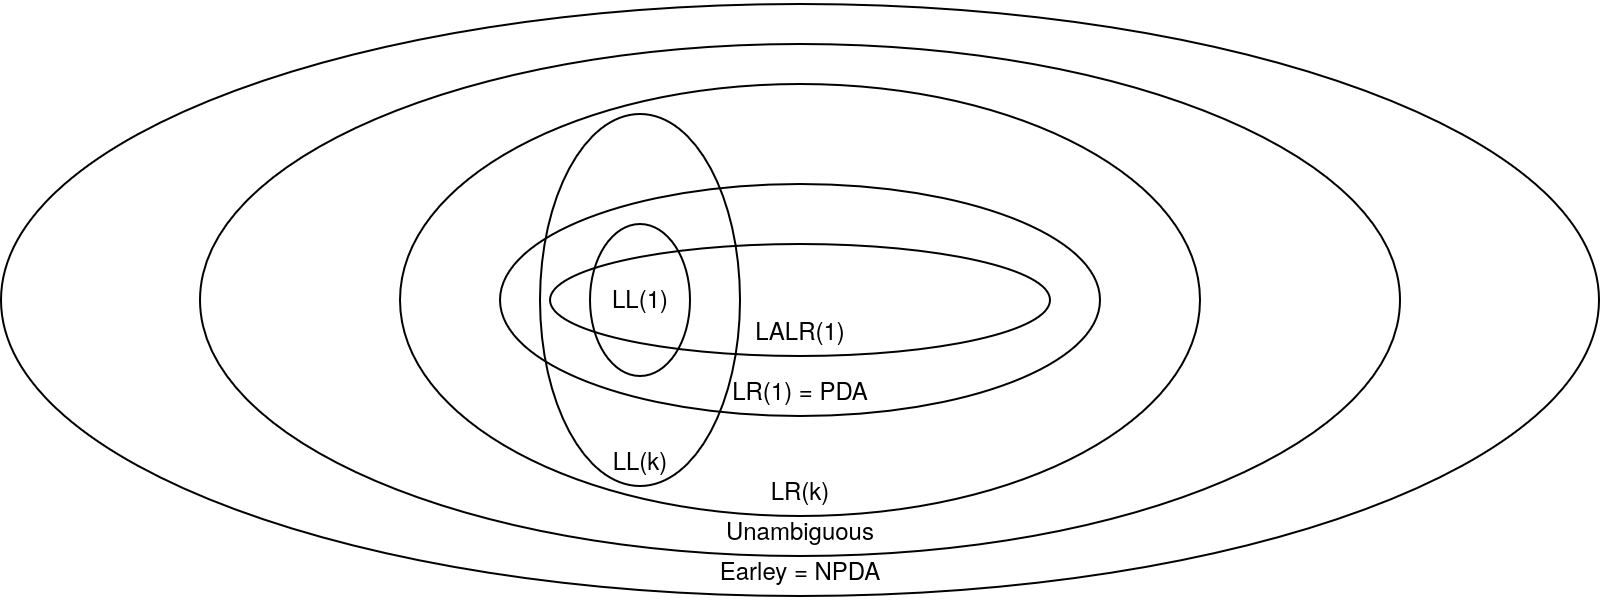
\includegraphics[scale=0.25]{chapters/grammars.png}
\centering
\end{figure}

\section{Conclusão}

Os algoritmos LR(1) e LALR(1) estendem o LR(0) e o SLR ao associar
lookaheads \textbf{locais} a cada item, em vez de usar o conjunto
FOLLOW global. O LR(1) é o mais preciso, mas gera o maior número de
estados. O LALR(1) oferece um equilíbrio excelente: funde estados
LR(1) com o mesmo núcleo, mantendo o número de estados igual ao
LR(0)/SLR e os lookaheads mais precisos que o SLR. Por isso, o
LALR(1) é o algoritmo de escolha para a maioria dos geradores de
analisadores sintáticos práticos.

\chapter{Geradores de analisadores sintáticos}

\section{Introdução}

No capítulo anterior estudamos os algoritmos LR(1) e LALR(1) de forma
teórica e implementamos suas tabelas em Haskell. Na prática, contudo,
construir essas tabelas à mão para uma gramática real seria
impraticável. Assim como o Alex automatiza a construção de
analisadores léxicos a partir de expressões regulares, o
\textbf{Happy} automatiza a construção de analisadores sintáticos a
partir de especificações gramaticais no estilo BNF. O Happy gera
analisadores LALR(1) e é a ferramenta padrão para este fim no
ecossistema Haskell: o próprio compilador GHC usa um parser gerado
pelo Happy.

Este capítulo apresenta o Happy através da especificação do parser de
expressões aritméticas, disponível em
\begin{flushleft}
  \verb|Exp/Frontend/Parser/Happy/ExpParser.y|
\end{flushleft}
Mostramos como cada parte do arquiv \texttt{.y} se
relaciona com os conceitos vistos nos capítulos anteriores e como
usar a opção \verb|-i| para inspecionar a tabela
LALR gerada. Por fim, ilustramos os dois tipos de conflito que podem
surgir em gramáticas ambíguas: conflitos shift-reduce e conflitos reduce-reduce.

\section{Estrutura de uma especificação Happy}

Um arquivo de especificação Happy (extensão .y) é dividido em quatro
partes, separadas
pelo marcador \%\%:

\begin{verbatim}
{ cabeçalho Haskell }

diretivas e declaração de tokens

%%

regras gramaticais

{ rodapé Haskell }
\end{verbatim}

\subsection{Cabeçalho}

A primeira seção, delimitada por chaves, contém código Haskell
puro que é copiado literalmente para
o início do arquivo gerado. É aqui que se declara o nome do módulo e
os imports necessários:

\begin{minted}{haskell}
{
module Exp.Frontend.Parser.Happy.ExpParser (expParser, parserTest) where

import Exp.Frontend.Lexer.Token
import Exp.Frontend.Lexer.Alex.ExpLexer hiding (lexer)
import Exp.Frontend.Syntax.ExpSyntax
}
\end{minted}

\subsection{Diretivas}

As diretivas configuram o parser gerado. As mais comuns são:

\begin{table}[H]
  \begin{tabular}{p{0.5\linewidth} p{0.5\linewidth}}
    \toprule
    Diretiva & Significado \\
    \midrule
    \verb|%name p N| & Gera a função \verb|p| que inicia o parsing
    pelo não-terminal \verb|N| \\
    \verb|%tokentype { T }| & Define o tipo Haskell dos tokens consumidos \\
    \verb|%monad { M }{ (>>=) }{ return }| & Executa o parser dentro
    da mônada \verb|M| \\
    \verb|%lexer { f }{ eof }| & Integra um lexer incremental;
    \verb|f| obtém o próximo token e \verb|eof|
    é o token de fim de entrada \\
    \verb|%error { h }| & Chama a função \verb|h| quando ocorre um
    erro de sintaxe \\
    \verb|%expect n| & Declara que a gramática possui exatamente
    \verb|n| conflitos shift-reduce esperados; o Happy falha se o
    número for diferente \\
    \bottomrule
  \end{tabular}
  \centering
\end{table}

No parser de expressões, essas diretivas ficam assim:

\begin{verbatim}
%name parser Exp
%monad {Alex}{(>>=)}{return}
%tokentype { Token }
%error     { parseError }
%lexer {lexer}{Token _ TEOF}
\end{verbatim}

A diretiva \verb|%monad| integra o Happy com a
mônada \verb|Alex| do lexer gerado pelo Alex. Com
\verb|%lexer|, o Happy chama a função
\haskell{lexer} cada vez que precisa de um token, em
vez de receber a lista completa de antemão. Esse modo incremental é
necessário quando o lexer é monádico.

\subsection{Declaração de tokens}

A seção \verb|%token| mapeia nomes simbólicos
usados nas regras gramaticais para padrões de correspondência (em
Haskell) contra o tipo de token. Cada linha tem a forma:

\begin{verbatim}
nome_simbólico  { padrão Haskell }
\end{verbatim}

No parser de expressões:

\begin{verbatim}
%token
      num       {Token _ (TNumber $$)}
      '('       {Token _ TLParen}
      ')'       {Token _ TRParen}
      '+'       {Token _ TPlus}
      '*'       {Token _ TTimes}
\end{verbatim}

O uso de \verb|$$| no padrão
\haskell{Token \_ (TNumber $$)} é especial: ele
captura o valor inteiro contido no token e o torna disponível nas
ações semânticas como \verb|$1|,
\verb|$2|, etc. Para tokens sem valor associado,
como \verb|TLParen|, o padrão apenas verifica que
o construtor bate.

\subsection{Declarações de precedência}

As declarações \verb|%left|,
\verb|%right| e
\verb|%nonassoc| servem para resolver conflitos
shift-reduce que surgem em gramáticas de expressões escritas de forma
ambígua. Cada linha associa uma precedência (determinada pela ordem
das declarações, de menor para maior) e uma associatividade a um ou mais tokens:

\begin{verbatim}
%left '+'
%left '*'
\end{verbatim}

Neste exemplo, \verb|*| tem precedência mais alta
que \verb|+| (pois aparece depois), e ambos são
associativos à esquerda. Veremos na seção sobre conflitos como essas
declarações eliminam a ambiguidade.

\subsection{Regras gramaticais}

Após o marcador \verb|%%|, definem-se as
produções da gramática no estilo BNF aumentado com ações semânticas em Haskell:

\begin{verbatim}
Exp : num         { EInt $1 }
    | Exp '+' Exp { $1 :+: $3 }
    | Exp '*' Exp { $1 :*: $3 }
    | '(' Exp ')' { $2 }
\end{verbatim}

Cada alternativa é uma produção seguida de uma ação entre chaves. Os
símbolos \verb|$1|, \verb|$2|,
\verb|$3| referem-se, respectivamente, ao
primeiro, segundo e terceiro símbolo do lado direito da produção. A
ação é executada quando o parser reduz por aquela produção,
construindo o nó correspondente da AST.

O tipo de retorno de cada não-terminal é inferido pelo compilador
Haskell a partir das ações: como \haskell{EInt $1} e
\haskell{$1 :+: $3} têm tipo
\haskell{Exp}, o não-terminal
\haskell{Exp} produz valores do tipo
\haskell{Exp}.

\subsection{Rodapé}

A última seção, também delimitada por chaves, contém funções
auxiliares usadas nas ações ou nas diretivas:

\begin{minted}{haskell}
{
parserTest :: String -> IO ()
parserTest s = do
  r <- expParser s
  print r

parseError (Token (line, col) lexeme)
  = alexError $ "Parse error while processing lexeme: " ++ show lexeme
                ++ "\n at line " ++ show line ++ ", column " ++ show col

lexer :: (Token -> Alex a) -> Alex a
lexer = (=<< alexMonadScan)

expParser :: String -> IO (Either String Exp)
expParser content = do
  pure $ runAlex content parser
}
\end{minted}

A função \haskell{parseError} recebe o token que
causou o erro e usa \haskell{alexError} para propagar
a mensagem de erro dentro da mônada Alex. A função
\haskell{lexer} adapta
\haskell{alexMonadScan} (que produz
\haskell{Alex Token}) para a interface esperada pelo
Happy (que recebe uma continuação
\haskell{Token -> Alex a}).

\section{Gerando o parser e inspecionando a tabela}

Para gerar o parser a partir da especificação, basta invocar o Happy:

\begin{minted}{bash}
happy ExpParser.y
happy -o ExpParser.hs ExpParser.y
\end{minted}

Quando a especificação faz parte de um projeto Cabal, o próprio Cabal
detecta arquivos .y em
\verb|build-tool-depends| (com
happy listado) e os processa
automaticamente antes da compilação Haskell.

\subsection{A opção -i}

A opção \verb|-i| instrui o Happy a gerar um
\textbf{arquivo de informação} (por padrão
\verb|ExpParser.info|) que descreve em detalhe a
tabela LALR construída:

\begin{minted}{bash}
happy -i ExpParser.y
\end{minted}

O arquivo gerado contém:

\begin{enumerate}
  \item
    \textbf{A gramática aumentada}: as produções numeradas,
    incluindo a produção inicial $S' \to Exp$.
  \item
    \textbf{Conjuntos FIRST} de cada não-terminal.
  \item
    \textbf{Os estados do autômato}: cada estado lista seus itens
    LR(1), com os lookaheads calculados pelo algoritmo LALR.
  \item
    \textbf{A tabela de ações}: para cada par (estado, terminal),
    a ação: shift, reduce ou accept.
  \item
    \textbf{A tabela goto}: para cada par (estado, não-terminal),
    o estado destino.
  \item
    \textbf{Conflitos}: se houver, eles são listados com o estado
    e o token envolvidos, indicando qual ação o Happy escolheu (por
    padrão, shift vence em conflitos shift-reduce).
\end{enumerate}

Este arquivo é extremamente útil para depurar gramáticas: ao ver em
qual estado um conflito ocorre e quais itens ele contém, é possível
identificar a ambiguidade na gramática e corrigi-la com declarações
de precedência ou reestruturando as produções.

\section{Conflitos shift-reduce}

Um conflito shift-reduce ocorre quando, em um determinado estado, o
parser pode tanto deslocar (shift) o próximo token quanto reduzir por
alguma produção. O caso mais comum é o de gramáticas de expressões
escritas de forma ambígua.

Considere a gramática de expressões \textbf{sem} declarações de precedência:

\begin{verbatim}
Exp : num
    | Exp '+' Exp
    | Exp '*' Exp
    | '(' Exp ')'
\end{verbatim}

Ao analisar a entrada \verb|1 + 2 * 3|, após ter
empilhado \verb|Exp '+' Exp| (com o segundo
\verb|Exp| valendo 2), o
parser vê * na entrada. Ele pode:

\begin{itemize}
  \item
    \textbf{Reduzir} \verb|Exp '+' Exp| para
    \verb|Exp| (interpretando
    \verb|(1 + 2) * 3|), ou
  \item
    \textbf{Deslocar} \verb|*| (interpretando
    \verb|1 + (2 * 3)|).
\end{itemize}

Sem orientação adicional, o Happy reporta o conflito e, por padrão,
escolhe sempre o shift. A mensagem no terminal seria:

\begin{verbatim}
ExpParser.y: shift/reduce conflicts:  4
\end{verbatim}

E no arquivo .info, cada conflito é
detalhado, por exemplo:

\begin{verbatim}
State 7

        Exp -> Exp . '+' Exp          (rule 2)
        Exp -> Exp . '*' Exp          (rule 3)
        Exp -> Exp '+' Exp .          (rule 2)

        '*'    shift, and enter state 5
               (reduce using rule 2)

        '+'    shift, and enter state 4
               (reduce using rule 2)

        ')'    reduce using rule 2
        '$'    reduce using rule 2
\end{verbatim}

A resolução correta é declarar precedência e associatividade antes do
\%\%. Ao escrevermos:

\begin{verbatim}
%left '+'
%left '*'
\end{verbatim}

o Happy usa essas informações para resolver cada conflito: quando o
token a deslocar tem precedência maior que a produção a reduzir, faz
shift; quando tem menor, reduz; quando são iguais, a associatividade
decide. Com as declarações acima, \verb|*| tem
precedência maior que \verb|+|, portanto
\verb|1 + 2 * 3| é interpretado como
\verb|1 + (2 * 3)|, e
\verb|%expect 0| pode ser declarado para
confirmar que nenhum conflito resta.

Outro exemplo clássico de conflito shift-reduce é o do \textbf{else
pendente} (\emph{dangling else}), presente em linguagens com
construção \verb|if-then-else| opcional:

\begin{verbatim}
Stmt : 'if' Exp 'then' Stmt
     | 'if' Exp 'then' Stmt 'else' Stmt
     | 'other'
\end{verbatim}

Ao analisar if e1 then if e2 then s1 else s2, após empilhar o
then interior, o parser vê else e tem dúvida: este
else pertence ao
if externo ou ao interno? Shift associa o
else ao if mais
próximo (interno), que é o comportamento convencional na maioria das
linguagens. A declaração \verb|%shift!| ou
simplesmente aceitar o comportamento padrão do Happy resolve o conflito.

\section{Conflitos reduce-reduce}

Um conflito reduce-reduce ocorre quando, em um determinado estado e
para um mesmo token de lookahead, dois itens completos diferentes
indicam reduções por produções distintas. Isso geralmente revela uma
ambiguidade estrutural na gramática que não pode ser resolvida por precedência.

Considere a gramática:

\begin{verbatim}
Expr : termo
     | termo

termo : 'x'
      | 'x'
\end{verbatim}

De forma mais realista, o conflito aparece quando dois não-terminais
distintos derivam a mesma sequência de terminais e são
intercambiáveis no mesmo contexto:

\begin{verbatim}
Prog : Decl
     | Expr

Decl : 'id'
Expr : 'id'
\end{verbatim}

Ao ver o token \verb|id| e precisar reduzir, o
parser não sabe se deve criar um nó \verb|Decl| ou
um nó \verb|Expr|. O arquivo
.info mostraria algo como:

\begin{verbatim}
State 1

        Decl -> 'id' .          (rule 1)
        Expr -> 'id' .          (rule 2)

        '$'    reduce using rule 1
               (reduce using rule 2)
\end{verbatim}

O Happy resolve o conflito escolhendo sempre a \textbf{primeira
regra} na ordem em que aparece no arquivo, mas emite um aviso.
Diferentemente dos conflitos shift-reduce, conflitos reduce-reduce
raramente têm uma resolução correta por padrão: eles quase sempre
indicam que a gramática precisa ser reformulada.

A solução mais comum é tornar os dois não-terminais sintáticos
distintos por contexto, introduzindo palavras-chave discriminadoras:

\begin{verbatim}
Prog : 'let' 'id'        -- declaração
     | 'id'              -- expressão
\end{verbatim}

Ou, alternativamente, desambiguar na fase semântica (análise de tipos
ou tabela de símbolos), como fazem as gramáticas de linguagens como
C, onde typedef torna certos
identificadores indistinguíveis de tipos sem informação de contexto.

\section{Conclusão}

Este capítulo apresentou o Happy, o gerador de analisadores
sintáticos padrão em Haskell. Vimos como um arquivo
.y é estruturado em quatro partes
(cabeçalho, diretivas, regras e rodapé) e como cada diretiva
configura o parser gerado. Estudamos a especificação concreta do
parser de expressões aritméticas, que integra o Happy com o lexer
monádico gerado pelo Alex. Mostramos como a opção
-i permite inspecionar os estados LALR e os
conflitos detectados, tornando o processo de depuração de gramáticas
transparente. Por fim, ilustramos os dois tipos de conflito
(shift-reduce, geralmente resolúvel com declarações de precedência, e
reduce-reduce, que normalmente exige a reformulação da gramática),
conectando os conceitos teóricos dos capítulos anteriores à prática
do desenvolvimento de compiladores em Haskell.

\part{Semântica formal e interpretadores}
\chapter{Introdução à semântica operacional}

\section{Introdução}

Até agora, estudamos como reconhecer se uma sequência de tokens
pertence a uma linguagem: a análise léxica e sintática. O próximo
passo é atribuir \textbf{significado} aos programas reconhecidos:
dado um programa sintaticamente correto, o que ele \emph{faz}? Essa
pergunta é o objeto de estudo da \textbf{semântica de linguagens de
programação}.

Existem várias maneiras de formalizar o significado de um programa.
Neste capítulo, estudaremos a \textbf{semântica operacional}, que
define o significado de um programa descrevendo como ele é
\emph{executado}, passo a passo, por uma máquina abstrata. A
semântica operacional é particularmente útil para a construção de
compiladores e interpretadores, pois a sua especificação se traduz
diretamente em código.

Apresentamos dois estilos de semântica operacional, ambos para uma
linguagem de expressões aritméticas com adição, multiplicação e
números inteiros:

\begin{itemize}
  \item
    \textbf{Small-step} (\emph{pequenos passos}): define a execução
    como uma sequência de reduções elementares, cada uma
    simplificando a expressão um pouco.
  \item
    \textbf{Big-step} (\emph{grandes passos}): define diretamente o
    valor final de uma expressão, abstraindo os passos intermediários.
\end{itemize}

Por fim, mostramos como a semântica big-step se traduz em um
interpretador Haskell, disponível em

\begin{flushleft}
  \verb|Exp/Interp/ExpInterp.hs|
\end{flushleft}

\section{A Linguagem de Expressões}

A linguagem que estudaremos é formada por três construções: números
inteiros, adição e multiplicação. Sua sintaxe abstrata pode ser
descrita pela gramática:

\[
  \begin{array}{lcl}
    e & ::= & n \mid e_1 + e_2 \mid e_1 * e_2
  \end{array}
\]

onde \(n\) representa um número inteiro. Em Haskell, o tipo de dado
correspondente é:

\begin{minted}{haskell}
data Exp
  = EInt Int
  | Exp :+: Exp
  | Exp :*: Exp
\end{minted}

Os construtores infixos \haskell{(:+:)} e
\haskell{(:*:)} refletem diretamente a estrutura
binária das operações.

\section{Semântica Small-Step}

A semântica \textbf{small-step} (ou semântica de redução) define a
execução de uma expressão como uma sequência de passos de
simplificação. Cada passo é descrito por uma \textbf{relação de
redução} \(e \to e'\), que se lê ``a expressão \(e\) reduz em um
passo para \(e'\)''.

\subsection{Valores}

Antes de apresentar as regras, precisamos distinguir as expressões
que já chegaram ao seu resultado final, os \textbf{valores},
das que ainda podem ser reduzidas. Para a linguagem de expressões
aritméticas, o único tipo de valor é um número inteiro:

\[
  v ::= n
\]

\subsection{Regras de Redução}

As regras de redução são apresentadas na forma de um sistema de
inferência. Cada regra tem a forma:

\[
  \infer[_{\{Nome\}}]{\text{conclusão}}{\text{premissas}}
\]

Se não houver premissas, a regra é um \textbf{axioma} e é escrita sem
a linha horizontal. Para a linguagem de expressões, temos as seguintes regras:

\textbf{Adição de valores:}

\[
  \infer[_{\{Add\}}]{n_1 + n_2 \to n_1 \mathbin{\hat{+}} n_2}{}
\]

onde \(\mathbin{\hat{+}}\) denota a adição aritmética de inteiros
(para distinguir o operador da linguagem do operador matemático).

\textbf{Redução no lado esquerdo da adição:}

\[
  \infer[_{\{AddL\}}]{e_1 + e_2 \to e_1' + e_2}{e_1 \to e_1'}
\]

\textbf{Redução no lado direito da adição:}

\[
  \infer[_{\{AddR\}}]{n_1 + e_2 \to n_1 + e_2'}{e_2 \to e_2'}
\]

A regra (AddR) só se aplica quando o lado esquerdo já é um valor
\(n_1\), garantindo uma ordem de avaliação da esquerda para a direita.

As regras para multiplicação são análogas:

\[
  \infer[_{\{Mul\}}]{n_1 * n_2 \to n_1 \mathbin{\hat{*}} n_2}{}
\]

\[
  \infer[_{\{MulL\}}]{e_1 * e_2 \to e_1' * e_2}{e_1 \to e_1'}
\]

\[
  \infer[_{\{MulR\}}]{n_1 * e_2 \to n_1 * e_2'}{e_2 \to e_2'}
\]

\subsection{Sequências de Redução}

A execução completa de uma expressão é uma sequência de reduções que
termina em um valor:

\[
  e \to e_1 \to e_2 \to \cdots \to v
\]

Escrevemos \(e \to^* v\) quando existe tal sequência (zero ou mais
passos). Para uma expressão que já é um valor, temos \(v \to^* v\)
com zero passos.

\subsection{Exemplo: Small-Step}

Considere a expressão \((2 + 3) * 4\). A redução small-step procede assim:

\[
  (2 + 3) * 4 \xrightarrow{\text{MulL}} 5 * 4 \xrightarrow{\text{Mul}} 20
\]

O passo 1 usa (MulL) com premissa \(2 + 3 \to 5\) (pela regra Add). O
passo 2 usa (Mul) diretamente, pois ambos os operandos já são valores.

Considere agora \(1 + 2 * 3\). Aplicando (AddL) e depois (MulL):

\[
  1 + 2 * 3
  \xrightarrow{\text{AddR}} 1 + 6
  \xrightarrow{\text{Add}} 7
\]

Note que a regra (AddR) se aplica porque o lado esquerdo \(1\) já é
um valor, forçando a avaliação do subtermos \(2 * 3\) antes da soma.

\section{Semântica Big-Step}

A semântica \textbf{big-step} (ou semântica natural) define
diretamente a relação entre uma expressão e o seu valor final,
abstraindo todos os passos intermediários. A relação é escrita \(e
\Downarrow v\), que se lê ``a expressão \(e\) avalia para o valor \(v\)''.

\subsection{Regras de Avaliação}

\textbf{Um número avalia para si mesmo:}

\[
  \infer[_{\{Num\}}]{n \Downarrow n}{}
\]

\textbf{Adição:}

\[
  \infer[_{\{Add\}}]{e_1 + e_2 \Downarrow n_1 \mathbin{\hat{+}}
  n_2}{e_1 \Downarrow n_1 & e_2 \Downarrow n_2}
\]

\textbf{Multiplicação:}

\[
  \infer[_{\{Mul\}}]{e_1 * e_2 \Downarrow n_1 \mathbin{\hat{*}}
  n_2}{e_1 \Downarrow n_1 & e_2 \Downarrow n_2}
\]

A estrutura é mais direta que a semântica small-step: cada regra
corresponde exatamente a um construtor da árvore sintática, e as
premissas avaliam recursivamente os sub-termos.

\subsection{Exemplos: Big-Step}

\textbf{Exemplo 1:} \((2 + 3) * 4 \Downarrow 20\)

A derivação é uma árvore de inferência:

\[
  \dfrac{
    \dfrac{
      \dfrac{}{2 \Downarrow 2} \quad \dfrac{}{3 \Downarrow 3}
    }{2 + 3 \Downarrow 5}
    \quad
    \dfrac{}{4 \Downarrow 4}
  }{(2 + 3) * 4 \Downarrow 20}
\]

\textbf{Exemplo 2:} \(1 + 2 * 3 \Downarrow 7\)

\[
  \dfrac{
    \dfrac{}{1 \Downarrow 1}
    \quad
    \dfrac{
      \dfrac{}{2 \Downarrow 2} \quad \dfrac{}{3 \Downarrow 3}
    }{2 * 3 \Downarrow 6}
  }{1 + 2 * 3 \Downarrow 7}
\]

Note que a árvore reflete diretamente a estrutura da árvore sintática
abstrata da expressão, é exatamente essa correspondência que torna
a semântica big-step tão conveniente para a implementação de interpretadores.

\section{Implementação em Haskell}

A semântica big-step se traduz em Haskell de forma quase literal.
Cada regra de inferência corresponde a uma equação da função
\haskell{eval}:

\begin{minted}{haskell}
module Exp.Interp.ExpInterp (eval) where

import Exp.Frontend.Syntax.ExpSyntax

eval :: Exp -> Int
eval (EInt n)    = n
eval (e1 :+: e2) = eval e1 + eval e2
eval (e1 :*: e2) = eval e1 * eval e2
\end{minted}

A correspondência com as regras semânticas é direta:

\begin{itemize}
  \item A equação \haskell{eval (EInt n) = n} implementa
    a regra (Num): um número \(n\) avalia para si mesmo.
  \item A equação \haskell{eval (e1 :+: e2) = eval e1 + eval e2} implementa
    a regra (Add): avalia recursivamente \(e_1\)
    e \(e_2\) e soma os resultados.
  \item A equação \haskell{eval (e1 :*: e2) = eval e1 * eval e2} implementa
    a regra (Mul) da mesma forma.
\end{itemize}

O casamento de padrões (pattern matching) de Haskell corresponde às
premissas de cada regra, e a chamada recursiva a
\haskell{eval} corresponde a aplicar a regra à sub-expressão.

\subsection{Executando o Interpretador}

O interpretador é parte do compilador
\haskell{exp}. Para usá-lo em modo de interpretação,
basta invocar:

\begin{verbatim}
cabal run exp -- --interp --file input.exp
\end{verbatim}

onde \verb|input.exp| contém uma expressão na
linguagem. Por exemplo, para a entrada

\begin{verbatim}
(2 + 3) * 4
\end{verbatim}

o interpretador produz \haskell{20}, confirmando o
resultado que calculamos pelas derivações semânticas acima.

\subsection{Totalidade e Terminação}

A função \haskell{eval} é \textbf{total}: está
definida para todas as expressões do tipo
\haskell{Exp} e sempre termina. Isso pode ser
verificado observando que cada chamada recursiva é feita sobre
sub-expressões estritamente menores, a estrutura da árvore
sintática abstrata diminui a cada nível. Essa propriedade é garantida
pela indução estrutural e corresponde, na semântica, ao fato de que
toda expressão da linguagem possui um valor (não há expressões que
ficam presas sem produzir resultado).

\section{Conclusão}

Neste capítulo, introduzimos a semântica operacional como ferramenta
para definir o significado de programas. Estudamos dois estilos
complementares:

\begin{itemize}
  \item
    A \textbf{semântica small-step} expõe cada passo de redução
    individualmente, permitindo raciocinar sobre o processo de execução.
  \item
    A \textbf{semântica big-step} relaciona expressões diretamente
    aos seus valores finais e se traduz quase literalmente em uma
    função recursiva Haskell.
\end{itemize}

A implementação do interpretador \haskell{eval}
demonstra que uma especificação semântica formal não é apenas um
documento teórico: ela é um projeto de implementação preciso. Nos
próximos capítulos, estenderemos esta linguagem com variáveis,
comandos e funções, exigindo que a semântica modele também
\textbf{ambientes} e \textbf{efeitos}.

\chapter{Semântica operacional para estado}

\section{Introdução}

No capítulo anterior, estudamos a semântica operacional de uma
linguagem de expressões aritméticas puras. Naquela linguagem, o valor
de uma expressão depende apenas da sua estrutura sintática: não há
variáveis, não há memória, não há efeitos colaterais. A execução é,
portanto, uma função pura: dada a expressão, o resultado é unicamente
determinado.

Programas reais, contudo, manipulam \textbf{estado}: valores são
armazenados em variáveis, lidos da entrada e escritos na saída. Para
modelar formalmente esse comportamento, a semântica operacional
precisa ser estendida com um componente que representa o estado da
memória em cada momento da execução.

Este capítulo estende a linguagem de expressões com
\textbf{variáveis} e apresenta uma linguagem de \textbf{comandos}
simples, a linguagem \emph{Line},  que inclui atribuição,
leitura da entrada padrão e impressão. Definimos a semântica
small-step e big-step para essa linguagem e mostramos como a
especificação semântica se traduz diretamente no interpretador
disponível em
\begin{flushleft}
  \verb|Line/Interp/LineInterp.hs|.
\end{flushleft}

\section{A Linguagem Line}

A linguagem \emph{Line} é uma linguagem imperativa mínima. Um
programa é uma sequência de comandos (instruções) que são executados
em ordem. A sua sintaxe abstrata é:

\[
  \begin{array}{lcl}
    \mathit{prog} & ::= & s^*\\
    s & ::= & x \mathbin{:=} e \\
    & \mid & \mathbf{read}\; x \\
    & \mid & \mathbf{print}\; e\\
    e & ::= & n \mid x \mid e_1 + e_2 \mid e_1 * e_2
  \end{array}
\]

onde \(n\) é um inteiro, \(x\) é um nome de variável e \(s^*\) denota
uma sequência (possivelmente vazia) de comandos.

Em Haskell, esses tipos são definidos como:

\begin{minted}{haskell}
data Line = Line [Stmt]

data Stmt
  = SAssign Var Exp
  | SRead   Var
  | SPrint  Exp

data Exp
  = EInt Int
  | EVar Var
  | Exp :+: Exp
  | Exp :*: Exp

type Var = String
\end{minted}

\section{Ambientes}

Para dar significado a um programa que usa variáveis, precisamos de
uma noção de \textbf{ambiente} (uma representação da memória): uma
função parcial \(\sigma : \mathit{Var}
\rightharpoonup \mathbb{Z}\) que mapeia nomes de variáveis para os
seus valores inteiros atuais.

Escrevemos:

\begin{itemize}
  \item \(\sigma(x)\) para o valor de \(x\) em \(\sigma\) (supondo \(x
    \in \mathrm{dom}(\sigma)\))
  \item \(\sigma[x \mapsto n]\) para o ambiente obtido de \(\sigma\)
    atualizando (ou inserindo) a variável \(x\) com o valor \(n\)
  \item \(\emptyset\) para o ambiente vazio (sem variáveis definidas)
\end{itemize}

Em Haskell, o ambiente é representado como
\haskell{Map String Int} do módulo
\haskell{Data.Map}.

\section{Semântica Small-Step}

\subsection{Expressões}

A avaliação de expressões não modifica o ambiente: expressões são
\textbf{puras} no sentido de que apenas consultam \(\sigma\), sem
alterá-lo. Uma configuração de expressão é um par \((\sigma, e)\) e a
relação de redução é \((\sigma, e) \to (\sigma, e')\).

\textbf{Variável:}

\[
  \infer[_{\{Var\}}]{(\sigma,\, x) \to (\sigma,\, \sigma(x))}{x \in
  \mathrm{dom}(\sigma)}
\]

Uma variável é substituída pelo seu valor corrente no ambiente. Se
\(x\) não estiver definida em \(\sigma\), a avaliação trava: erro
de variável não inicializada.

\textbf{Redução de subexpressões:}

\[
  \begin{array}{cc}
    \infer[_{\{AddL\}}]{(\sigma,\, e_1 + e_2) \to (\sigma,\, e_1' +
    e_2)}{(\sigma, e_1) \to (\sigma, e_1')}
    &
    \infer[_{\{AddR\}}]{(\sigma,\, n_1 + e_2) \to (\sigma,\, n_1 +
    e_2')}{(\sigma, e_2) \to (\sigma, e_2')}
  \end{array}
\]

\[
  \infer[_{\{Add\}}]{(\sigma,\, n_1 + n_2) \to (\sigma,\, n_1
  \mathbin{\hat{+}} n_2)}{}
\]

As regras para multiplicação são análogas: (MulL), (MulR) e (Mul).

\subsection{Comandos}

A configuração de um comando inclui o ambiente, pois os comandos
podem modificá-lo. Usamos a notação \((\sigma, s) \to (\sigma',
s')\), onde \(s'\) é o comando residual após a redução. Quando um
comando termina sua execução, dizemos que ele reduz para
\(\mathbf{skip}\), um comando que não faz nada.

\textbf{Atribuição: avalia a expressão primeiro:}

\[
  \infer[_{\{AssignStep\}}]{(\sigma,\, x \mathbin{:=} e)\to
  (\sigma,\, x \mathbin{:=} e')}{(\sigma, e) \to (\sigma, e')}
\]

\textbf{Atribuição: expressão já é um valor:}

\[
  \infer[_{\{Assign\}}]{(\sigma,\, x \mathbin{:=} n) \to (\sigma[x \mapsto n],\,
  \mathbf{skip})}{}
\]

\textbf{Impressão: avalia a expressão primeiro:}

\[
  \infer[_{\{PrintStep\}}]{(\sigma,\, \mathbf{print}\; e)\to
  (\sigma,\, \mathbf{print}\; e')}{(\sigma, e) \to (\sigma, e')}
\]

\textbf{Impressão: expressão já é um valor:}

\[
  \infer[_{\{Print\}}]{(\sigma,\, \mathbf{print}\; n) \to (\sigma,\,
  \mathbf{skip})}{}
  \quad [\text{ emite $n$ na saída}]
\]

\textbf{Sequência:}

\[
  \infer[_{\{SeqSkip\}}]{(\sigma,\, \mathbf{skip};\, s^\star) \to
  (\sigma,\, s^\star)}{}
\]

\[
  \infer[_{\{Seq\}}]{(\sigma,\, s;\, s^\star) \to (\sigma',\, s';\,
  s^\star)}{(\sigma, s) \to (\sigma', s')}
\]

\subsection{Exemplo: Small-Step}

Considere o programa:

\begin{verbatim}
x := 2 + 3
print x * 4
\end{verbatim}

Iniciamos com o ambiente vazio \(\emptyset\). A execução procede assim:

\[
  (\emptyset,\; x \mathbin{:=} 2 + 3;\; \mathbf{print}\; x * 4)
\] \[
  \xrightarrow{\text{Seq, Add}} ([x \mapsto 5],\; \mathbf{skip};\;
  \mathbf{print}\; x * 4)
\] \[
  \xrightarrow{\text{SeqSkip}} ([x \mapsto 5],\; \mathbf{print}\; x * 4)
\] \[
  \xrightarrow{\text{PrintStep, Var}} ([x \mapsto 5],\; \mathbf{print}\; 5 * 4)
\] \[
  \xrightarrow{\text{PrintStep, Mul}} ([x \mapsto 5],\; \mathbf{print}\; 20)
\] \[
  \xrightarrow{\text{Print}} ([x \mapsto 5],\; \mathbf{skip}) \quad
  \text{[emite 20]}
\]

Cada passo é justificado por uma regra; a sequência termina quando
restam apenas \(\mathbf{skip}\)s.

\section{Semântica Big-Step}

Na semântica big-step, abstraímos os passos intermediários e
definimos diretamente a relação entre configuração inicial e resultado final.

\subsection{Expressões}

A relação \(\sigma \vdash e \Downarrow n\) significa ``no ambiente
\(\sigma\), a expressão \(e\) avalia para o inteiro \(n\)''.

\textbf{Número:}

\[
  \infer[_{\{Num\}}]{\sigma \vdash n \Downarrow n}{}
\]

\textbf{Variável:}

\[
  \infer[_{\{Var\}}]{\sigma \vdash x \Downarrow \sigma(x)}{x \in
  \mathrm{dom}(\sigma)}
\]

\textbf{Adição:}

\[
  \infer[_{\{Add\}}]{\sigma \vdash e_1 + e_2 \Downarrow n_1
  \mathbin{\hat{+}} n_2}{\sigma \vdash e_1 \Downarrow n_1 & \sigma
  \vdash e_2 \Downarrow n_2}
\]

\textbf{Multiplicação:}

\[
  \infer[_{\{Mul\}}]{\sigma \vdash e_1 * e_2 \Downarrow n_1
  \mathbin{\hat{*}} n_2}{\sigma \vdash e_1 \Downarrow n_1 & \sigma
  \vdash e_2 \Downarrow n_2}
\]

\subsection{Comandos}

A relação \(\sigma, s \Downarrow \sigma'\) significa ``executar o
comando \(s\) no ambiente \(\sigma\) produz o ambiente \(\sigma'\)''.
O ambiente é o único ``resultado'' de um comando; os efeitos de I/O
(impressão, leitura) são considerados efeitos colaterais implícitos.

\textbf{Atribuição:}

\[
  \infer[_{\{Assign\}}]{\sigma,\; x \mathbin{:=} e \;\Downarrow\;
  \sigma[x \mapsto n]}{\sigma \vdash e \Downarrow n}
\]

\textbf{Impressão:}

\[
  \infer[_{\{Print\}}]{\sigma,\; \mathbf{print}\; e \;\Downarrow\;
  \sigma}{\sigma \vdash e \Downarrow n}
\]

O ambiente não muda com \haskell{print}; apenas o
valor de \(e\) é emitido como efeito colateral.

\textbf{Leitura:}

\[
  \infer[_{\{Read\}}]{\sigma,\; \mathbf{read}\; x \;\Downarrow\;
  \sigma[x \mapsto n]}{}
  \quad n \text{ lido da entrada}
\]

A regra (Read) é um axioma cuja premissa implícita é a leitura de um
inteiro \(n\) da entrada padrão.

\textbf{Sequência vazia:}

\[
  \infer[_{\{SeqNil\}}]{\sigma,\; \epsilon \;\Downarrow\; \sigma}{}
\]

\textbf{Sequência não-vazia:}

\[
  \infer[_{\{SeqCons\}}]{\sigma,\; s;\, s^* \;\Downarrow\;
  \sigma''}{\sigma,\; s \;\Downarrow\; \sigma' \quad \sigma',\; s^*
  \;\Downarrow\; \sigma''}
\]

\subsection{Exemplos: Big-Step}\label{exemplos-big-step}

\textbf{Exemplo 1:} Derivação para \haskell{x := 2 +
3} partindo de \(\emptyset\).

\[
  \dfrac{
    \dfrac{
      \dfrac{}{\emptyset \vdash 2 \Downarrow 2}
      \quad
      \dfrac{}{\emptyset \vdash 3 \Downarrow 3}
    }{\emptyset \vdash 2 + 3 \Downarrow 5}
  }{\emptyset,\; x \mathbin{:=} 2 + 3 \;\Downarrow\; [x \mapsto 5]}
\]

\textbf{Exemplo 2:} Derivação para o programa completo
(\haskell{x := 2 + 3; print x * 4}) partindo de \(\emptyset\).

\[
  \dfrac{
    \underbrace{\emptyset,\; x \mathbin{:=} 2+3 \;\Downarrow\; [x
    \mapsto 5]}_{\text{Exemplo 1}}
    \quad
    \dfrac{
      \dfrac{
        \dfrac{}{[x\mapsto 5] \vdash x \Downarrow 5}
        \quad
        \dfrac{}{[x\mapsto 5] \vdash 4 \Downarrow 4}
      }{[x\mapsto 5] \vdash x \star 4 \Downarrow 20}
    }{[x\mapsto 5],\; \mathbf{print}\; x\star 4 \;\Downarrow\; [x\mapsto 5]}
  }{\emptyset,\; x \mathbin{:=} 2+3;\; \mathbf{print}\; x\star 4
  \;\Downarrow\; [x\mapsto 5]}
\]

A derivação confirma que, ao final, \(x = 5\) e o valor \(20\) foi emitido.

\section{Implementação em Haskell}

\subsection{O Ambiente como Mônada de Estado}

A semântica big-step dita que cada comando recebe um ambiente e
produz um (possivelmente diferente) ambiente. Em Haskell, isso é
capturado pela \textbf{mônada de estado} (\haskell{StateT}):

\begin{minted}{haskell}
type Env = Map String Int
type Interp a = ExceptT String (StateT Env IO) a
\end{minted}

A pilha de mônadas combina três capacidades:
\begin{itemize}
  \item \haskell{StateT Env}: o ambiente \(\sigma\)
    implícito, que pode ser lido com \haskell{get} e
    atualizado com \haskell{modify};
  \item  \haskell{ExceptT String}: tratamento de erros
    (como variável não definida) via \haskell{throwError}
  \item \haskell{IO}: efeitos de I/O para
    \haskell{read} e \haskell{print}.
\end{itemize}

O ponto de entrada executa a pilha a partir do ambiente vazio:

\begin{minted}{haskell}
interp :: Line -> IO ()
interp p = do
    (r, _) <- runStateT (runExceptT (interpProgram p)) Map.empty
    case r of
      Left err -> putStrLn err
      Right _  -> pure ()
\end{minted}

\subsection{Interpretador de Expressões}

A função \haskell{interpExp} implementa as regras
(Num), (Var), (Add) e (Mul):

\begin{minted}{haskell}
interpExp :: Exp -> Interp Int
interpExp (EInt n) = pure n
interpExp (EVar v) = askVar v
interpExp (e1 :+: e2) = (+) <$> interpExp e1 <*> interpExp e2
interpExp (e1 :*: e2) = (*) <$> interpExp e1 <*> interpExp e2
\end{minted}

A função auxiliar \haskell{askVar} implementa a regra
(Var): consulta o ambiente corrente e lança um erro se a variável não
estiver definida (caso não coberto pelas regras semânticas):

\begin{minted}{haskell}
askVar :: String -> Interp Int
askVar s = do
    env <- get
    case Map.lookup s env of
      Nothing  -> throwError $ unwords ["Undefined variable:", s]
      Just val -> pure val
\end{minted}

\subsection{Interpretador de Comandos}

A função \haskell{interpStmt} implementa as regras
(Assign), (Print) e (Read):

\begin{minted}{haskell}
interpStmt :: Stmt -> Interp ()
interpStmt (SAssign v e) = do
    val <- interpExp e
    updateVar v val
interpStmt (SRead v) = do
    str <- liftIO getLine
    let val = read str
    updateVar v val
interpStmt (SPrint e) = do
    val <- interpExp e
    liftIO $ print val
\end{minted}

A correspondência com as regras semânticas é direta:

\begin{itemize}
  \item \haskell{SAssign v e}: avalia
    \haskell{e} (regra Assign, premissa) e
    atualiza o ambiente com \haskell{updateVar}
    (conclusão: \(\sigma[x \mapsto n]\)).
  \item \haskell{SPrint e}: avalia
    \haskell{e} e imprime o resultado; o ambiente não
    muda (regra Print).
  \item \haskell{SRead v}: lê um inteiro da entrada
    padrão e armazena em \haskell{v} (regra Read).
\end{itemize}

A função \haskell{updateVar} encapsula a operação
\(\sigma[x \mapsto n]\):

\begin{minted}{haskell}
updateVar :: String -> Int -> Interp ()
updateVar s val = modify (Map.insert s val)
\end{minted}

A interpretação de um programa aplica
\haskell{interpStmt} a cada comando em sequência,
correspondendo às regras (SeqNil) e (SeqCons):

\begin{minted}{haskell}
interpProgram :: Line -> Interp ()
interpProgram (Line ss) = mapM_ interpStmt ss
\end{minted}

\haskell{mapM_} sequencia os comandos na ordem e
descarta os resultados unitários, o que equivale exatamente a
encadear as regras (SeqCons) até atingir (SeqNil).

\subsection{Executando o Interpretador}

\begin{verbatim}
cabal run line -- --interp --file programa.line
\end{verbatim}

Por exemplo, dado o arquivo \haskell{programa.line}:

\begin{verbatim}
x := 10
y := x * 2
print y
\end{verbatim}

O interpretador produziria 20.

\section{Conclusão}

Neste capítulo, estendemos a semântica operacional para lidar com
\textbf{estado}, introduzindo ambientes que mapeiam variáveis a
valores. As contribuições principais foram:

\begin{itemize}
  \item
    A \textbf{semântica small-step} para comandos usa configurações
    \((\sigma, s)\) que transportam o ambiente ao longo dos passos de
    redução. A regra (Assign) modifica o ambiente na transição; as
    outras regras o propagam sem alteração.
  \item
    A \textbf{semântica big-step} relaciona um comando e um ambiente
    inicial ao ambiente final, abstraindo os passos intermediários. A
    sua estrutura de ``entrada → saída de ambiente'' traduz-se
    diretamente na mônada de estado de Haskell.
  \item
    A \textbf{implementação} em
    LineInterp.hs usa a pilha
    \haskell{ExceptT String (StateT Env IO)}, que
    integra estado (ambiente), erros e I/O. Cada equação do
    interpretador corresponde a uma regra semântica.
\end{itemize}

O padrão estado-como-mônada que vimos aqui reaparecerá nos próximos
capítulos quando estendermos a linguagem com estruturas de controlo
como condicionais e laços.

\chapter{Semântica operacional para uma linguagem imperativa simples}

\section{Introdução}

No capítulo anterior, definimos a semântica operacional da linguagem
\emph{Line}, que inclui atribuição, leitura e impressão. Com isso, já
conseguimos modelar programas que executam uma sequência fixa de
comandos. No entanto, programas reais precisam de \textbf{controle de
fluxo}: executar blocos diferentes dependendo de uma condição, e
repetir um bloco enquanto uma condição permanecer verdadeira.

Este capítulo estende a linguagem com \textbf{condicionais}
(if/else) e \textbf{repetição}
(while), formando a linguagem \emph{While}.
Para suportar condições, a linguagem de expressões também é estendida
com \textbf{valores booleanos} e operações de comparação. Definimos a
semântica small-step e big-step para todas as novas construções e
mostramos como essa especificação se traduz no interpretador
disponível em
\begin{flushleft}
  \verb|While/Interp/WhileInterp.hs|
\end{flushleft}

\section{A Linguagem While}

A linguagem \emph{While} estende \emph{Line} com dois novos comandos
e uma classe de expressões booleanas. A sua sintaxe abstrata é:

\[
  \begin{array}{lcl}
    \mathit{prog} & ::= & s^\star\\
    s & ::= & x \mathbin{:=} e
    \mid \mathbf{read}\; x
    \mid \mathbf{print}\; e \\
    &    & \mid\; \mathbf{if}\; e\; \mathbf{then}\; \{s^\star\}\;
    \mathbf{else}\; \{s^\star\} \\
    &    & \mid\; \mathbf{while}\; e\; \mathbf{do}\; \{s^\star\} \\
    e & ::= & v \mid x
    \mid e_1 + e_2 \mid e_1 \star e_2 \\
    &    & \mid\; e_1 < e_2 \mid e_1 = e_2 \mid e_1 \mathbin{|} e_2
    \mid \neg e \\
    v & ::= & n \mid \mathbf{true} \mid \mathbf{false}
  \end{array}
\]

Os valores agora incluem inteiros e booleanos. Em Haskell:

\begin{minted}{haskell}
data Value
  = VInt  Int
  | VBool Bool

data Exp
  = EValue Value
  | EVar   Var
  | Exp :+: Exp  -- adição
  | Exp :*: Exp  -- multiplicação
  | Exp :<: Exp  -- menor que
  | Exp :=: Exp  -- igualdade
  | Exp :|: Exp  -- disjunção
  | ENot Exp     -- negação

data Stmt
  = SAssign Var Exp
  | SRead   Var
  | SPrint  Exp
  | SIf    Exp Block Block
  | SWhile Exp Block

type Block = [Stmt]
\end{minted}

\section{Ambientes}

O ambiente \(\sigma : \mathit{Var} \rightharpoonup \mathit{Val}\)
agora associa variáveis a \textbf{valores} (inteiros ou booleanos).
A notação \(\sigma(x)\), \(\sigma[x \mapsto v]\) e \(\emptyset\) é a
mesma do capítulo anterior.

\section{Semântica Small-Step}

\subsection{Expressões}

Os valores \(v\) são as formas terminais; qualquer expressão que
não seja um valor pode ainda ser reduzida. As regras para adição e
multiplicação são idênticas ao capítulo anterior. As novas regras
tratam das operações booleanas.

\textbf{Variável:}

\[
  \infer[_{\{Var\}}]{(\sigma,\, x) \to (\sigma,\, \sigma(x))}{x \in
  \mathrm{dom}(\sigma)}
\]

\textbf{Redução de subexpressões:}

Para cada operador binário \(\oplus\), as regras (OpL) e (OpR)
reduzem o operando esquerdo primeiro e depois o direito,
preservando o ambiente:

\[
  \begin{array}{cc}
    \infer[_{\{OpL\}}]{(\sigma,\, e_1 \oplus e_2)\to (\sigma,\, e_1'
    \oplus e_2)}{(\sigma, e_1) \to (\sigma, e_1')}
    &
    \infer[_{\{OpR\}}]{(\sigma,\, v_1 \oplus e_2)\to (\sigma,\, v_1
    \oplus e_2')}{(\sigma, e_2) \to (\sigma, e_2')}
  \end{array}
\]

\textbf{Operações sobre valores:}

\[
  \begin{array}{cc}
    \infer[_{\{Add\}}]{(\sigma,\, n_1 + n_2) \to (\sigma,\, n_1
        \mathbin{\hat{+}}
    n_2)}{}
    &
    \infer[_{\{Mul\}}]{(\sigma,\, n_1 \star n_2) \to (\sigma,\, n_1
    \mathbin{\hat{\star}} n_2)}{}
  \end{array}
\]

\[
  \begin{array}{cc}
    \infer[_{\{Lt\}}]{(\sigma,\, n_1 < n_2) \to (\sigma,\, n_1 \mathbin{\hat{<}}
    n_2)}{}
    &
    \infer[_{\{Eq\}}]{(\sigma,\, v_1 = v_2) \to (\sigma,\, v_1 \mathbin{\hat{=}}
    v_2)}{}
  \end{array}
\]

\[
  \begin{array}{cc}
    \infer[_{\{Or\}}]{(\sigma,\, b_1 \mathbin{|} b_2) \to (\sigma,\, b_1
    \mathbin{\hat{\lor}} b_2)}{}
    &
    \infer[_{\{Not\}}]{(\sigma,\, \neg b) \to (\sigma,\, \hat{\neg}\, b)}{}\\ \\
    \multicolumn{2}{c}{
      \infer[_{\{NotStep\}}]{(\sigma,\, \neg e) \to (\sigma,\, \neg
      e')}{(\sigma,\, e) \to (\sigma,\, e')}
    }
  \end{array}
\]

Os operadores com acento (\(\hat{+}\), \(\hat{<}\), \(\hat{\lor}\),
etc.) denotam as operações matemáticas correspondentes, para
distingui-las dos operadores da linguagem.

\subsection{Comandos}

As regras para \haskell{SAssign},
\haskell{SRead}, \haskell{SPrint} e
para sequências são as mesmas do capítulo anterior. As novas regras
tratam de \haskell{if} e \haskell{while}.

\textbf{Condicional: avaliação da condição}

\[
  \infer[_{\{IfStep\}}]{(\sigma,\; \mathbf{if}\; e\;
    \mathbf{then}\; B_1\; \mathbf{else}\; B_2) \to (\sigma,\;
      \mathbf{if}\; e'\; \mathbf{then}\; B_1\; \mathbf{else}\;
  B_2)}{(\sigma, e) \to (\sigma, e')}
\]

\textbf{Condicional: ramo verdadeiro}

\[
  \infer[_{\{IfTrue\}}]{(\sigma,\; \mathbf{if}\; \mathbf{true}\; \mathbf{then}\;
  B_1\; \mathbf{else}\; B_2) \to (\sigma,\; B_1)}{}
\]

\textbf{Condicional: ramo falso}

\[
  \infer[_{\{IfFalse\}}]{(\sigma,\; \mathbf{if}\; \mathbf{false}\;
      \mathbf{then}\;
  B_1\; \mathbf{else}\; B_2) \to (\sigma,\; B_2)}{}
\]

\textbf{While: iteração}

A regra chave para while é a de
\textbf{iteração condicional}: o laço se transforma em um condicional que,
no ramo verdadeiro, executa o corpo e depois o laço novamente.

\[
  \infer[_{\{While\}}]{(\sigma,\; \mathbf{while}\; e\; \mathbf{do}\; B) \to
    (\sigma,\; \mathbf{if}\; e\; \mathbf{then}\; (B;\; \mathbf{while}\;
  e\; \mathbf{do}\; B)\; \mathbf{else}\; \epsilon)}{}
\]

onde \(\epsilon\) denota a sequência vazia. Esta regra captura a
semântica de repetição de forma simples: o
while se reduz a um condicional cujo ramo
verdadeiro contém o corpo seguido do próprio while.

\subsection{Exemplo: Small-Step}

Considere o programa:

\begin{verbatim}
i := 0
while i < 3 do { i := i + 1 }
print i
\end{verbatim}

Partindo de \(\emptyset\), após a atribuição inicial temos \(\sigma_0
= [i \mapsto 0]\). Mostramos os passos de uma iteração do laço:

\[
  (\sigma_0,\; \mathbf{while}\; i < 3\; \mathbf{do}\; \{i
  \mathbin{:=} i+1\})
\] \[
  \xrightarrow{\text{While}}
  (\sigma_0,\; \mathbf{if}\; i < 3\; \mathbf{then}\; \{i \mathbin{:=}
  i+1;\; \mathbf{while}\ldots\}\; \mathbf{else}\; \epsilon)
\] \[
  \xrightarrow{\text{IfStep, Var, Lt}}
  (\sigma_0,\; \mathbf{if}\; \mathbf{true}\; \mathbf{then}\; \{i
  \mathbin{:=} i+1;\; \mathbf{while}\ldots\}\; \mathbf{else}\; \epsilon)
\] \[
  \xrightarrow{\text{IfTrue}}
  (\sigma_0,\; i \mathbin{:=} i+1;\; \mathbf{while}\; i < 3\;
  \mathbf{do}\; \{i \mathbin{:=} i+1\})
\] \[
  \xrightarrow{\text{Assign}}
  ([i \mapsto 1],\; \mathbf{while}\; i < 3\; \mathbf{do}\; \{i
  \mathbin{:=} i+1\})
\]

Após três iterações, \(\sigma = [i \mapsto 3]\). Na quarta, a
condição \(3 < 3\) reduz para \(\mathbf{false}\) e a regra (IfFalse)
seleciona \(\epsilon\), terminando o laço.

\subsection{Extensão TImp: Semântica Small-Step}\label{sec:timp-small-step}

A linguagem \emph{TImp} estende \emph{While} com construções de
registro e funções. As regras small-step para registros seguem o
mesmo padrão das construções já apresentadas; a semântica completa de
chamadas de função é especificada na forma big-step na
Seção~\ref{sec:timp-big-step}, pois o comando \haskell{return}
exigiria um modelo de pilha de chamadas para ser tratado em small-step.

As configurações passam a incluir o ambiente de funções \(\Phi\):
\((\sigma, \Phi, e)\) para expressões e \((\sigma, \Phi, s)\) para
comandos.

\paragraph{Construção de registro.}

Os campos são avaliados da esquerda para a direita. Enquanto houver
um campo não-valor, ele é reduzido (NewStep); quando todos os campos
são valores, o registro é construído (New):

\[
  \infer[_{\{NewStep\}}]
  {(\sigma, \Phi,\;
    \mathbf{new}\; R\,\{f_1\!=\!v_1,\ldots,f_i\!=\!e_i,\ldots\})
    \to (\sigma', \Phi,\;
  \mathbf{new}\; R\,\{f_1\!=\!v_1,\ldots,f_i\!=\!e_i',\ldots\})}
  {(\sigma, \Phi,\, e_i) \to (\sigma', \Phi,\, e_i')}
\]

\[
  \infer[_{\{New\}}]
  {(\sigma, \Phi,\; \mathbf{new}\; R\,\{f_1\!=\!v_1,\ldots,f_n\!=\!v_n\})
    \to (\sigma, \Phi,\;
  \mathbf{rec}(R,\,\{f_1 \mapsto v_1,\ldots,f_n \mapsto v_n\}))}
  {}
\]

\paragraph{Acesso a campo.}

\[
  \infer[_{\{FieldStep\}}]
  {(\sigma, \Phi,\; e.f) \to (\sigma', \Phi,\; e'.f)}
  {(\sigma, \Phi,\, e) \to (\sigma', \Phi,\, e')}
\]

\[
  \infer[_{\{Field\}}]
  {(\sigma, \Phi,\; \mathbf{rec}(R,\mathit{flds}).f) \to
  (\sigma, \Phi,\; \mathit{flds}(f))}
  {f \in \mathrm{dom}(\mathit{flds})}
\]

\paragraph{Declaração de variável.}

\[
  \infer[_{\{DeclStep\}}]
  {(\sigma, \Phi,\; \mathbf{var}\; x \mathbin{:} \tau = e) \to
  (\sigma', \Phi,\; \mathbf{var}\; x \mathbin{:} \tau = e')}
  {(\sigma, \Phi,\, e) \to (\sigma', \Phi,\, e')}
\]

\[
  \infer[_{\{Decl\}}]
  {(\sigma, \Phi,\; \mathbf{var}\; x \mathbin{:} \tau = v) \to
  (\sigma[x \mapsto v],\; \Phi,\; \epsilon)}
  {}
\]

\paragraph{Atribuição de campo.}

\[
  \infer[_{\{FieldAssignStep\}}]
  {(\sigma, \Phi,\; x.f \mathbin{:=} e) \to
  (\sigma', \Phi,\; x.f \mathbin{:=} e')}
  {(\sigma, \Phi,\, e) \to (\sigma', \Phi,\, e')}
\]

\[
  \infer[_{\{FieldAssign\}}]
  {(\sigma, \Phi,\; x.f \mathbin{:=} v)
    \to (\sigma[x \mapsto \mathbf{rec}(R,\,\mathit{flds}[f \mapsto
  v])],\; \Phi,\; \epsilon)}
  {\sigma(x) = \mathbf{rec}(R,\mathit{flds})}
\]

\paragraph{Avaliação de argumentos.}

Os argumentos de uma chamada de função são avaliados da esquerda para
a direita antes da invocação. A regra de invocação — que cria um
ambiente de ativação fresco e executa o corpo — é especificada na
forma big-step:

\[
  \infer[_{\{CallStep\}}]
  {(\sigma, \Phi,\;
    f(v_1,\ldots,v_{i-1},e_i,\ldots,e_n)) \to
    (\sigma', \Phi,\;
  f(v_1,\ldots,v_{i-1},e_i',\ldots,e_n))}
  {(\sigma, \Phi,\, e_i) \to (\sigma', \Phi,\, e_i')}
\]

\section{Semântica Big-Step}

\subsection{Expressões}

A relação \(\sigma \vdash e \Downarrow v\) agora produz um
\textbf{valor} (inteiro ou booleano).

\[
  \begin{array}{cc}
    \infer[_{\{Val\}}]{\sigma \vdash v \Downarrow v}{}
    &
    \infer[_{\{Var\}}]{\sigma \vdash x
    \Downarrow \sigma(x)}{x \in \mathrm{dom}(\sigma)}
  \end{array}
\]

\[
  \begin{array}{cc}
    \infer[_{\{Add\}}]{\sigma \vdash e_1 + e_2 \Downarrow n_1
    \mathbin{\hat{+}} n_2}{\sigma \vdash e_1 \Downarrow n_1 & \sigma \vdash e_2
    \Downarrow n_2}
    &
    \infer[_{\{Mul\}}]{\sigma \vdash e_1 \star e_2 \Downarrow n_1
    \mathbin{\hat{\star}} n_2}{\sigma \vdash e_1 \Downarrow n_1 &
    \sigma \vdash e_2\Downarrow n_2}
  \end{array}
\]

\[
  \begin{array}{cc}
    \infer[_{\{Lt\}}]{\sigma \vdash e_1 < e_2 \Downarrow n_1
    \mathbin{\hat{<}} n_2}
    {\sigma \vdash e_1 \Downarrow n_1 \quad \sigma \vdash e_2
    \Downarrow n_2}
    &
    \infer[_{\{Eq\}}]{\sigma \vdash e_1 = e_2 \Downarrow v_1
    \mathbin{\hat{=}} v_2}{\sigma \vdash e_1 \Downarrow v_1 & \sigma \vdash e_2
    \Downarrow v_2}
  \end{array}
\]

\[
  \begin{array}{cc}
    \infer[_{\{Or\}}]{\sigma \vdash e_1 \mathbin{|} e_2 \Downarrow b_1
    \mathbin{\hat{\lor}} b_2}{\sigma \vdash e_1 \Downarrow b_1 &
      \sigma \vdash e_2
    \Downarrow b_2}
    &
    \infer[_{\{Not\}}]{\sigma \vdash \neg e \Downarrow \hat{\neg}\, b}
    {\sigma \vdash e \Downarrow b}
  \end{array}
\]

\subsection{Comandos}

As regras para \haskell{SAssign},
\haskell{SRead}, \haskell{SPrint},
(SeqNil) e (SeqCons) permanecem iguais ao capítulo anterior. As novas
regras são:

\textbf{Condicional: ramo verdadeiro}

\[
  \infer[_{\{IfTrue\}}]{\sigma,\; \mathbf{if}\; e\; \mathbf{then}\;
    B_1\; \mathbf{else}\;
  B_2 \;\Downarrow\; \sigma'}{\sigma \vdash e \Downarrow
    \mathbf{true} \quad \sigma,\; B_1
  \Downarrow \sigma'}
\]

\textbf{Condicional: ramo falso}

\[
  \infer[_{\{IfFalse\}}]{\sigma,\; \mathbf{if}\; e\; \mathbf{then}\;
    B_1\; \mathbf{else}\;
  B_2 \;\Downarrow\; \sigma'}{\sigma \vdash e \Downarrow
    \mathbf{false} \quad \sigma,\; B_2
  \Downarrow \sigma'}
\]

\textbf{While: condição falsa (terminação)}

\[
  \infer[_{\{WhileFalse\}}]{\sigma,\; \mathbf{while}\; e\;
  \mathbf{do}\; B \;\Downarrow\; \sigma}
  {\sigma \vdash e \Downarrow \mathbf{false}}
\]

\textbf{While: condição verdadeira (iteração)}

\[
  \infer[_{\{WhileTrue\}}]{\sigma,\; \mathbf{while}\; e\;
  \mathbf{do}\; B \;\Downarrow\; \sigma''}
  {\sigma \vdash e \Downarrow \mathbf{true}
    &  \sigma,\; B \Downarrow \sigma'
  & \sigma',\; \mathbf{while}\; e\; \mathbf{do}\; B \Downarrow \sigma''}
\]

A regra (WhileTrue) é recursiva: após executar o corpo \(B\) e obter
\(\sigma'\), o while é aplicado novamente a
partir de \(\sigma'\). A recursão termina quando a condição se torna
\(\mathbf{false}\), coberta por (WhileFalse). Se a condição nunca se
tornar falsa, não existe derivação big-step finita: o programa diverge.

\subsection{Exemplos: Big-Step}

\textbf{Exemplo 1:} Considere o seguinte programa:

\begin{verbatim}
if 2 < 3 then {
  x := 10;
} else {
  x := 20;
}
\end{verbatim}

\[
  \dfrac{
    \dfrac{
      \dfrac{}{\emptyset \vdash 2 \Downarrow 2}
      \quad
      \dfrac{}{\emptyset \vdash 3 \Downarrow 3}
    }{\emptyset \vdash 2 < 3 \Downarrow \mathbf{true}}
    \quad
    \dfrac{
      \dfrac{}{\emptyset \vdash 10 \Downarrow 10}
    }{\emptyset,\; x \mathbin{:=} 10 \;\Downarrow\; [x \mapsto 10]}
  }{\emptyset,\; \mathbf{if}\; 2<3\; \mathbf{then}\; \{x \mathbin{:=}
    10\}\; \mathbf{else}\; \{x \mathbin{:=} 20\} \;\Downarrow\; [x
  \mapsto 10]}
\]

\textbf{Exemplo 2:} Considere o programa:

\begin{verbatim}
while i < 2 do {
   i := i + 1;
}
\end{verbatim}
e o estado inicial \(\sigma_0 = [i \mapsto 0]\).

Abreviemos \(\sigma_k = [i \mapsto k]\) e o programa anterior
por \(W\).

\[
  \dfrac{
    \sigma_0 \vdash i < 2 \Downarrow \mathbf{true}
    \quad
    \sigma_0,\; i \mathbin{:=} i+1 \;\Downarrow\; \sigma_1
    \quad
    \dfrac{
      \sigma_1 \vdash i < 2 \Downarrow \mathbf{true}
      \quad
      \sigma_1,\; i \mathbin{:=} i+1 \;\Downarrow\; \sigma_2
      \quad
      \dfrac{
        \sigma_2 \vdash i < 2 \Downarrow \mathbf{false}
      }{\sigma_2,\; W \;\Downarrow\; \sigma_2}
    }{\sigma_1,\; W \;\Downarrow\; \sigma_2}
  }{\sigma_0,\; W \;\Downarrow\; \sigma_2}
\]

A derivação é uma árvore de profundidade proporcional ao número de
iterações. O laço termina porque \(i\) cresce a cada iteração e
eventualmente atinge 2.

\subsection{Extensão TImp: Semântica Big-Step}\label{sec:timp-big-step}

A linguagem \emph{TImp} estende \emph{While} com declarações de
funções e tipos registro. Nesta seção apresentamos os domínios
semânticos e as regras big-step para as novas construções.

\subsubsection{Sintaxe Estendida}

Um programa TImp consiste em uma sequência de declarações seguida de
um bloco de comandos de nível superior:

\[
  \begin{array}{lcl}
    \mathit{prog}  & ::= & \mathit{decl}^*\; s^* \\[4pt]
    \mathit{decl}  & ::= &
    \mathbf{record}\; R\; \{\, \overline{f_i \mathbin{:} \tau_i}\,\}  \\
    & \mid &
    \mathbf{fn}\; f\,(\overline{x_i \mathbin{:} \tau_i}) \mathbin{:}
    \rho\; \{\, s^*\,\} \\[4pt]
    \rho           & ::= & \mathbf{void} \mid \tau \\[4pt]
    \tau           & ::= & \mathbf{int} \mid \mathbf{bool} \mid
    \mathbf{string} \mid R \\[4pt]
    s              & ::= & \cdots \mid
    \mathbf{var}\; x \mathbin{:} \tau \mathbin{=} e \mid
    x.f \mathbin{:=} e \mid
    \mathbf{return}\; e \mid \mathbf{return} \mid
    f(e_1,\ldots,e_n) \\[4pt]
    e              & ::= & \cdots \mid e.f \mid
    \mathbf{new}\; R\,\{\,\overline{f_i \mathbin{=} e_i}\,\} \mid
    f(e_1,\ldots,e_n)
  \end{array}
\]

Os reticências \(\cdots\) denotam as construções já presentes em
\emph{While}.

\subsubsection{Domínios Semânticos Estendidos}

\paragraph{Valores.}
O domínio de valores é estendido com valores registro e com o valor
unitário (resultado de funções \haskell{void}):

\[
  v \;::=\; n \;\mid\; b \;\mid\; s \;\mid\;
  \mathbf{rec}(R,\, \{f_1 \mapsto v_1, \ldots, f_n \mapsto v_n\})
  \;\mid\; \mathbf{unit}
\]

Um valor registro \(\mathbf{rec}(R, \mathit{flds})\) carrega o nome do
tipo \(R\) e uma função parcial \(\mathit{flds}\) que mapeia nomes de
campo a valores. A semântica adota \textbf{semântica de valor} para
registros: toda atribuição e passagem de parâmetro copia o registro
inteiro.

\paragraph{Ambientes de funções.}
Além do ambiente de variáveis \(\sigma\), a semântica introduz um
\textbf{ambiente de funções} global

\[
  \Phi : \mathit{Name} \rightharpoonup
  (\overline{x_i},\; B)
\]

que mapeia cada nome de função à sua lista de parâmetros formais
\(\overline{x_i}\) e ao seu corpo \(B\). O ambiente \(\Phi\) é
construído uma única vez a partir das declarações do programa e
permanece imutável durante a execução.

\paragraph{Resultado de bloco.}
As construções \haskell{return} interrompem a execução normal de um
bloco e devolvem um valor ao chamador. Para modelar esse comportamento,
a relação de avaliação de comandos e blocos passa a produzir um
\textbf{resultado}:

\[
  r \;::=\; \mathbf{normal} \;\mid\; {\uparrow}\, v
\]

O resultado \(\mathbf{normal}\) indica terminação sem retorno; o
resultado \({\uparrow}\, v\) indica que um \haskell{return} foi
executado e o valor \(v\) está sendo propagado para o ponto de chamada.
A relação de avaliação de comandos torna-se \(\sigma,\Phi \vdash s
\Downarrow (\sigma', r)\) e a de blocos, \(\sigma,\Phi \vdash B
\Downarrow (\sigma', r)\).

\subsubsection{Semântica Big-Step: Registros}

\paragraph{Expressões}

\textbf{Construção de registro:}

\[
  \infer[_{\{\mathit{New}\}}]
  {\sigma,\Phi \vdash \mathbf{new}\; R\,\{f_1\!=\!e_1,\ldots,f_n\!=\!e_n\}
  \Downarrow \mathbf{rec}(R,\,\{f_1 \mapsto v_1,\ldots,f_n \mapsto v_n\})}
  {\sigma,\Phi \vdash e_1 \Downarrow v_1
    \quad \cdots \quad
  \sigma,\Phi \vdash e_n \Downarrow v_n}
\]

Cada campo é avaliado na ordem em que aparece na expressão.

\textbf{Acesso a campo:}

\[
  \infer[_{\{\mathit{Field}\}}]
  {\sigma,\Phi \vdash e.f \Downarrow \mathit{flds}(f)}
  {\sigma,\Phi \vdash e \Downarrow \mathbf{rec}(R,\mathit{flds})
  \quad f \in \mathrm{dom}(\mathit{flds})}
\]

O acesso avalia \(e\) para um valor registro e extrai o campo \(f\).
Se \(f\) não existir, a execução trava (erro de tipo prevenido pela
verificação de tipos).

\paragraph{Comandos}

\textbf{Declaração de variável:}

\[
  \infer[_{\{\mathit{Decl}\}}]
  {\sigma,\Phi \vdash \mathbf{var}\; x \mathbin{:} \tau \mathbin{=} e
  \Downarrow (\sigma[x \mapsto v],\; \mathbf{normal})}
  {\sigma,\Phi \vdash e \Downarrow v}
\]

\textbf{Atribuição de campo:}

\[
  \infer[_{\{\mathit{FieldAssign}\}}]
  {\sigma,\Phi \vdash x.f \mathbin{:=} e
    \Downarrow (\sigma[x \mapsto \mathbf{rec}(R,\,\mathit{flds}[f
      \mapsto v])],\;
  \mathbf{normal})}
  {\sigma(x) = \mathbf{rec}(R,\mathit{flds})
  \quad \sigma,\Phi \vdash e \Downarrow v}
\]

A atribuição não aloca um novo registro: ela atualiza o registro em
\(x\) substituindo o campo \(f\) pelo novo valor \(v\). Como a
semântica é de valor, \(x\) recebe uma cópia modificada.

\subsubsection{Semântica Big-Step: Funções}

\paragraph{Propagação de \texttt{return}}

Para que \haskell{return} interrompa a execução de um bloco, as
regras de sequência precisam propagar o resultado.

\textbf{Bloco vazio:}

\[
  \infer[_{\{\mathit{BlkNil}\}}]
  {\sigma,\Phi \vdash \epsilon \Downarrow (\sigma,\; \mathbf{normal})}
  {}
\]

\textbf{Bloco com retorno antecipado:}

\[
  \infer[_{\{\mathit{BlkRet}\}}]
  {\sigma,\Phi \vdash s\,;\,B \Downarrow (\sigma',\; {\uparrow}\,v)}
  {\sigma,\Phi \vdash s \Downarrow (\sigma',\; {\uparrow}\,v)}
\]

Se o primeiro comando produz um retorno, o resto do bloco \(B\) não é
executado e o resultado é propagado imediatamente.

\textbf{Bloco com continuação normal:}

\[
  \infer[_{\{\mathit{BlkCons}\}}]
  {\sigma,\Phi \vdash s\,;\,B \Downarrow r}
  {\sigma,\Phi \vdash s \Downarrow (\sigma',\; \mathbf{normal})
  \quad \sigma',\Phi \vdash B \Downarrow r}
\]

\paragraph{Comandos de retorno}

\textbf{Retorno com valor:}

\[
  \infer[_{\{\mathit{RetVal}\}}]
  {\sigma,\Phi \vdash \mathbf{return}\; e \Downarrow (\sigma,\; {\uparrow}\,v)}
  {\sigma,\Phi \vdash e \Downarrow v}
\]

\textbf{Retorno sem valor (\texttt{void}):}

\[
  \infer[_{\{\mathit{RetVoid}\}}]
  {\sigma,\Phi \vdash \mathbf{return} \Downarrow (\sigma,\;
  {\uparrow}\,\mathbf{unit})}
  {}
\]

\paragraph{Chamada de função}

\textbf{Chamada como expressão} (função não-\texttt{void}):

\[
  \infer[_{\{\mathit{CallExpr}\}}]
  {\sigma,\Phi \vdash f(e_1,\ldots,e_n) \Downarrow v}
  {
    \Phi(f) = (\overline{x_i},\; B)
    \quad
    \sigma,\Phi \vdash e_i \Downarrow v_i \;\;(\forall\, i)
    \quad
    [x_1 \mapsto v_1,\ldots,x_n \mapsto v_n],\Phi \vdash B
    \Downarrow (\_,\; {\uparrow}\,v)
  }
\]

O corpo de \(f\) é executado em um \textbf{ambiente fresco}
\([x_1 \mapsto v_1,\ldots,x_n \mapsto v_n]\): apenas os parâmetros
formais estão em escopo. O resultado \({\uparrow}\,v\) fornece o valor
de retorno; o ambiente da chamada \(\sigma\) não é modificado.

\textbf{Chamada como comando} (função \texttt{void} ou retorno descartado):

\[
  \infer[_{\{\mathit{CallStmt}\}}]
  {\sigma,\Phi \vdash f(e_1,\ldots,e_n) \Downarrow (\sigma,\; \mathbf{normal})}
  {
    \Phi(f) = (\overline{x_i},\; B)
    \quad
    \sigma,\Phi \vdash e_i \Downarrow v_i \;\;(\forall\, i)
    \quad
    [x_1 \mapsto v_1,\ldots,x_n \mapsto v_n],\Phi \vdash B \Downarrow (\_,\; \_)
  }
\]

O ambiente de chamada é devolvido inalterado: a função não pode
alterar o estado externo através de variáveis globais mutáveis nem por
passagem por referência.

\section{Implementação em Haskell}

\subsection{Expressões}

A função \haskell{interpExp} retorna agora um
\haskell{Value} (inteiro ou booleano). As novas
equações implementam diretamente as regras semânticas:

\begin{minted}{haskell}
interpExp :: Exp -> Interp Value
interpExp (EValue v) = pure v
interpExp (EVar v) = askVar v
interpExp (e1 :+: e2) = do { v1 <- interpExp e1; v2 <- interpExp e2; v1 .+. v2 }
interpExp (e1 :*: e2) = do { v1 <- interpExp e1; v2 <- interpExp e2; v1 .*. v2 }
interpExp (e1 :<: e2) = do { v1 <- interpExp e1; v2 <- interpExp e2; v1 .<. v2 }
interpExp (e1 :=: e2) = do { v1 <- interpExp e1; v2 <- interpExp e2; v1 .=. v2 }
interpExp (e1 :|: e2) = do { v1 <- interpExp e1; v2 <- interpExp e2; v1 .|. v2 }
interpExp (ENot e) = do { v <- interpExp e; vnot v }
\end{minted}

As funções \haskell{(.+.)},
\haskell{(.<.)}, \haskell{(.=.)},
\haskell{(.|.)} e \haskell{vnot},
definidas em \haskell{Utils.Value}, verificam que os
operandos têm os tipos corretos e lançam um erro via
\haskell{throwError} caso contrário.

\subsection{Condicional}

A equação para \haskell{SIf} implementa as regras
(IfTrue) e (IfFalse):

\begin{minted}{haskell}
interpStmt (SIf e blk1 blk2) = do
    v <- interpExp e
    case v of
      VBool True  -> mapM_ interpStmt blk1
      VBool False -> mapM_ interpStmt blk2
      _           -> throwError $ unlines
                       ["Expecting a boolean value, but found:", pretty e]
\end{minted}

O casamento de padrões em \haskell{VBool True} e
\haskell{VBool False} corresponde diretamente às
premissas das regras (IfTrue) e (IfFalse). O caso
\haskell{_} trata erros de tipo que as regras
semânticas simplesmente não cobrem.

\subsection{Repetição}

A equação para \haskell{SWhile} implementa as regras
(WhileFalse) e (WhileTrue):

\begin{minted}{haskell}
interpStmt (SWhile e blk1) = do
    v <- interpExp e
    case v of
      VBool False -> pure ()
      VBool True  -> do
          mapM_ interpStmt blk1
          interpStmt (SWhile e blk1)
      _ -> throwError $ unlines
             ["Expecting a boolean value, but found:", pretty e]
\end{minted}

A correspondência com as regras semânticas é precisa:

\begin{itemize}
  \item
    \haskell{VBool False -> pure ()}, correspondendo à regra
    (WhileFalse): o ambiente não muda, a execução termina sem
    produzir nenhum efeito adicional.
  \item
    \haskell{VBool True -> mapM_ interpStmt blk1 >>
    interpStmt (SWhile e blk1)}, correspondendo à regra (WhileTrue): executa o
    bloco (\(\sigma, B \Downarrow \sigma'\)) e depois invoca
    \haskell{interpStmt (SWhile e blk1)}
    recursivamente (\(\sigma', \mathbf{while}\ldots \Downarrow \sigma''\)).
\end{itemize}

A recursão na implementação espelha a recursão na regra semântica: se
o laço não terminar, a função Haskell também não terminará.

\subsection{Executando o Interpretador}

\begin{verbatim}
cabal run while -- --interp --file programa.while
\end{verbatim}

Por exemplo, o seguinte programa calcula o fatorial de 5:

\begin{verbatim}
n := 5;
acc := 1;
while 0 < n do {
    acc := acc * n;
    n := n + (-1);
}
print acc;
\end{verbatim}

O interpretador imprime 120.

\subsection{Implementação da Extensão TImp}

A implementação está em \verb|TImp/Interp/TImpInterp.hs|. As regras
semânticas apresentadas na Seção~\ref{sec:timp-big-step} têm
correspondência direta com o código Haskell.

\paragraph{Domínio de valores e estado.}

\begin{minted}{haskell}
data Value
  = VInt    Int
  | VBool   Bool
  | VString String
  | VRecord Name (Map Field Value)  -- rec(R, flds)
  | VUnit                           -- unit

data InterpState = InterpState
  { varEnv  :: Map Var Value        -- sigma
  , funcEnv :: Map Name FuncDecl    -- Phi
  }

type InterpM a = StateT InterpState (ExceptT String IO) a
\end{minted}

O campo \haskell{funcEnv} corresponde ao ambiente global \(\Phi\),
construído uma vez no ponto de entrada e nunca modificado.

\paragraph{Resultado de bloco.}

A função \haskell{execBlock} retorna \haskell{Maybe Value},
onde \haskell{Nothing} corresponde a \(\mathbf{normal}\) e
\haskell{Just v} corresponde a \({\uparrow}\,v\):

\begin{minted}{haskell}
execBlock :: [Stmt] -> InterpM (Maybe Value)
execBlock []     = pure Nothing              -- BlkNil
execBlock (s:ss) = do
  r <- execStmt s
  case r of
    Just _  -> pure r                        -- BlkRet: propagate
    Nothing -> execBlock ss                  -- BlkCons: continue
\end{minted}

\paragraph{Registros.}

A avaliação de \haskell{ENew} implementa a regra (New):

\begin{minted}{haskell}
evalExp (ENew rname initFields) = do
  vals <- mapM (\(f, e) -> (f,) <$> evalExp e) initFields
  pure (VRecord rname (Map.fromList vals))
\end{minted}

O acesso a campo implementa a regra (Field):

\begin{minted}{haskell}
evalExp (EField e f) = do
  v <- evalExp e
  case v of
    VRecord _ fields ->
      case Map.lookup f fields of
        Just val -> pure val
        Nothing  -> throwError ("Record has no field: " ++ f)
    _ -> throwError "Field access on non-record value"
\end{minted}

A atribuição de campo implementa (FieldAssign):

\begin{minted}{haskell}
execStmt (SFieldAssign v f e) = do
  rval <- lookupVar v
  newVal <- evalExp e
  case rval of
    VRecord name fields ->
      let fields' = Map.insert f newVal fields
      in  modify (\st -> st
            { varEnv = Map.insert v (VRecord name fields') (varEnv st) })
    _ -> throwError (v ++ " is not a record")
  pure Nothing
\end{minted}

\paragraph{Funções.}

O comando \haskell{return} implementa as regras (RetVal) e (RetVoid):

\begin{minted}{haskell}
execStmt (SReturn Nothing)  = pure (Just VUnit)
execStmt (SReturn (Just e)) = Just <$> evalExp e
\end{minted}

A chamada de função implementa as regras (CallExpr) e (CallStmt).
A função auxiliar \haskell{callFunc} cria um novo ambiente e executa
o corpo:

\begin{minted}{haskell}
callFunc :: Name -> [Value] -> InterpM Value
callFunc fname argVals = do
  fenv <- gets funcEnv
  case Map.lookup fname fenv of
    Nothing -> throwError ("Undefined function: " ++ fname)
    Just (FuncDecl _ params _ body) -> do
      let bindings = zip [v | Param v _ <- params] argVals
      withFreshEnv bindings $ do        -- ambiente novo: sigma_0
        r <- execBlock body
        pure (fromMaybe VUnit r)        -- extrai v de (uparrow v)
\end{minted}

A função \haskell{withFreshEnv} salva o ambiente corrente, inicializa
o novo ambiente com apenas os parâmetros formais e restaura o ambiente
original ao terminar, implementando a semântica de escopo local:

\begin{minted}{haskell}
withFreshEnv :: [(Var, Value)] -> InterpM a -> InterpM a
withFreshEnv bindings m = do
  saved <- gets varEnv
  modify (\st -> st { varEnv = Map.fromList bindings })
  r <- m
  modify (\st -> st { varEnv = saved })
  pure r
\end{minted}

\section{Conclusão}

Neste capítulo, completámos a semântica operacional de uma linguagem
imperativa com as construções de controle de fluxo mais fundamentais:

\begin{itemize}
  \item
    O \textbf{condicional} é modelado por duas regras simétricas,
    (IfTrue) e (IfFalse), que selecionam o ramo a executar com base
    no valor booleano da condição.
  \item
    O \textbf{laço} while é modelado por
    (WhileFalse), que termina quando a condição é falsa, e
    (WhileTrue), que executa o corpo e recomeça: uma regra
    inerentemente recursiva que espelha a definição operacional
    de repetição.
  \item
    Na semântica small-step, o while se
    \textbf{desenrola} em um condicional, o que torna explícita a
    estrutura de cada iteração.
  \item
    Na semântica big-step, a não-terminação corresponde à ausência de
    uma derivação finita: a semântica é parcial por construção.
  \item
    \textbf{Registros} são modelados como valores estruturados
    \(\mathbf{rec}(R, \mathit{flds})\) com semântica de cópia; as regras
    (New), (Field) e (FieldAssign) cobrem criação, leitura e atualização.
  \item
    \textbf{Funções} introduzem o conceito de \textit{resultado de bloco}
    \(r \in \{\mathbf{normal}, {\uparrow}\,v\}\) para modelar
    \haskell{return}: as regras (BlkRet) e (BlkCons) propagam ou
    descartam esse resultado; (CallExpr) executa a função em um ambiente
    fresco e extrai o valor retornado.
\end{itemize}

A implementação em \verb|TImp/Interp/TImpInterp.hs| segue a
especificação semântica com precisão, confirmando que uma boa
especificação formal é também um guia de implementação direta.

\part{Sistemas e verificação de tipos}
\chapter{Introdução aos sistemas de tipos}

\section{Introdução}

Nos capítulos anteriores, definimos semânticas operacionais para
linguagens de expressões e para linguagens imperativas. Vimos que a
semântica de uma linguagem pode ser dada por regras de inferência que
descrevem como os programas são executados. No entanto, a semântica
por si só não impede que expressões sem sentido sejam escritas: como
somar um booleano a um inteiro, ou executar
\haskell{pred true}. Essas expressões são
\textbf{sintaticamente válidas}, mas \textbf{semanticamente sem significado}.

É exatamente para isso que servem os \textbf{sistemas de tipos}:
impor, de forma estática, que apenas expressões semanticamente
bem-definidas possam ser executadas. Este capítulo apresenta as
diferentes estratégias de tipagem utilizadas por linguagens de
programação e discute os sistemas de tipos, utilizados para descrever
formalmente regras para validação de tipos em linguagens de programação.

\section{Tipos em Linguagens de Programação}

Um \textbf{tipo} é uma classificação de valores que define:

\begin{enumerate}
  \item Quais operações são aplicáveis a eles;
  \item Como eles são representados na memória;
  \item Que conjunto de valores o tipo compreende.
\end{enumerate}

Por exemplo, o tipo \haskell{Int} classifica valores
inteiros e admite operações aritméticas; o tipo
\haskell{Bool} classifica os valores
\haskell{true} e \haskell{false} e
admite operações lógicas. O \textbf{sistema de tipos} de uma
linguagem é o conjunto de regras que associa tipos a expressões e
verifica se essas associações são coerentes.

\subsection{Tipagem Estática e Dinâmica}

A distinção mais fundamental em sistemas de tipos é \emph{quando} a
verificação de tipos ocorre:

\textbf{Tipagem estática} (\emph{static typing}): a verificação é
feita em \textbf{tempo de compilação}, antes da execução do programa.
Se o programa contiver um erro de tipo, o compilador o rejeita. As
linguagens Haskell, Java, C e Rust são exemplos que usam tipagem estática.

\textbf{Tipagem dinâmica} (\emph{dynamic typing}): a verificação é
feita em \textbf{tempo de execução}, à medida que o programa é
executado. Erros de tipo são detectados apenas quando a operação
inválida é executada. Exemplos de linguagens que usam essa estratégia
são Python, JavaScript, Ruby e Lisp.

A tipagem estática oferece garantias mais fortes: o sistema de tipos
pode certificar que certos tipos de erros \emph{nunca} ocorrerão em
nenhuma execução do programa. A tipagem dinâmica oferece mais
flexibilidade, mas adia a detecção de erros para o momento da execução.

\subsection{Tipagem Forte e Fraca}

Uma distinção ortogonal é a de \textbf{tipagem forte} vs \textbf{tipagem fraca}:

\textbf{Tipagem forte} (\emph{strong typing}): a linguagem não
permite conversões implícitas entre tipos incompatíveis. Operações
entre tipos diferentes resultam em erro (em tempo de compilação ou
execução). Exemplos: Haskell, Python.

\textbf{Tipagem fraca} (\emph{weak typing}): a linguagem realiza
conversões implícitas entre tipos, frequentemente de maneiras
surpreendentes. Exemplos: C (converte implicitamente entre inteiros e
ponteiros), JavaScript (\haskell{1 + "1"} resulta em
\haskell{"11"}).

Note que estas classificações são independentes: Python é
dinamicamente tipado e fortemente tipado; C é estaticamente tipado e
fracamente tipado.

\section{A Linguagem de Expressões Tipadas}

Para discutirmos sobre sistemas de tipos, vamos utilizar um linguagem
de expressões simples. A sua \textbf{sintaxe abstrata} é representada
pela seguinte gramática:

\[
  \begin{array}{lcll}
    t & ::= & \mathbf{true}  & \text{(verdadeiro)} \\
    & \mid & \mathbf{false} & \text{(falso)} \\
    & \mid & \mathbf{if}\ t_1\ \mathbf{then}\ t_2\ \mathbf{else}\ t_3
    & \text{(condicional)} \\
    & \mid & \mathbf{0} & \text{(zero)} \\
    & \mid & \mathbf{succ}\ t & \text{(sucessor)} \\
    & \mid & \mathbf{pred}\ t & \text{(predecessor)} \\
    & \mid & \mathbf{iszero}\ t & \text{(teste de zero)}
  \end{array}
\]

Os \textbf{tipos} são:

\[
  \begin{array}{lcll}
    T & ::= & \mathbf{Bool} & \text{(booleano)} \\
    & \mid & \mathbf{Nat}  & \text{(número natural)}
  \end{array}
\]

Os \textbf{valores} da linguagem são os termos que já não podem ser
reduzidos pela semântica operacional. Distinguimos dois tipos de valores:

\[
  \begin{array}{lcll}
    v & ::= & \mathbf{true} \mid \mathbf{false} \mid nv \\
    nv & ::= & \mathbf{0} \mid \mathbf{succ}\ nv
  \end{array}
\]

onde \(nv\) denota os \textbf{valores numéricos}, isto é, \(\mathbf{0}\) e
qualquer número de aplicações de \(\mathbf{succ}\) a \(\mathbf{0}\).

\section{O Sistema de Tipos}

Um \textbf{sistema de tipos} é definido por uma \textbf{relação de
tipagem} entre termos e tipos. Escrevemos \(\vdash t : T\) para dizer
que ``o termo \(t\) tem tipo \(T\)''. A relação é definida por um
conjunto de regras de inferência.

\subsection{Regras de Tipagem}

\textbf{Constantes booleanas:}

\[
  \frac{}{\vdash \mathbf{true} : \mathbf{Bool}} \quad\text{(T-True)}
  \qquad
  \frac{}{\vdash \mathbf{false} : \mathbf{Bool}} \quad\text{(T-False)}
\]

\textbf{Condicional:}

\[
  \frac{
    \vdash t_1 : \mathbf{Bool} \quad
    \vdash t_2 : T \quad
    \vdash t_3 : T
  }{
    \vdash \mathbf{if}\ t_1\ \mathbf{then}\ t_2\ \mathbf{else}\ t_3 : T
  } \quad\text{(T-If)}
\]

A regra (T-If) exige que a condição \(t_1\) seja booleana e que os
dois ramos \(t_2\) e \(t_3\) tenham o \textbf{mesmo tipo} \(T\). O
resultado do condicional tem esse tipo.

\textbf{Naturais:}

\[
  \frac{}{\vdash \mathbf{0} : \mathbf{Nat}} \quad\text{(T-Zero)}
\]

\[
  \frac{\vdash t_1 : \mathbf{Nat}}{\vdash \mathbf{succ}\ t_1 :
  \mathbf{Nat}} \quad\text{(T-Succ)}
  \qquad
  \frac{\vdash t_1 : \mathbf{Nat}}{\vdash \mathbf{pred}\ t_1 :
  \mathbf{Nat}} \quad\text{(T-Pred)}
\]

\[
  \frac{\vdash t_1 : \mathbf{Nat}}{\vdash \mathbf{iszero}\ t_1 :
  \mathbf{Bool}} \quad\text{(T-IsZero)}
\]

\subsection{Exemplos de Derivações de Tipo}

\textbf{Exemplo 1:} O termo
\(\mathbf{iszero}\ (\mathbf{succ}\ \mathbf{0})\) tem tipo \(\mathbf{Bool}\):

\[
  \dfrac{
    \dfrac{
      \dfrac{}{\vdash \mathbf{0} : \mathbf{Nat}}
    }{\vdash \mathbf{succ}\ \mathbf{0} : \mathbf{Nat}}
  }{\vdash \mathbf{iszero}\ (\mathbf{succ}\ \mathbf{0}) : \mathbf{Bool}}
\]

\textbf{Exemplo 2:} O condicional
\(\mathbf{if}\ (\mathbf{iszero}\ \mathbf{0})\ \mathbf{then}\ \mathbf{0}\ \mathbf{else}\ \mathbf{succ}\ \mathbf{0}\)
tem tipo \(\mathbf{Nat}\):

\[
  \dfrac{
    \dfrac{
      \dfrac{}{\vdash \mathbf{0} : \mathbf{Nat}}
    }{\vdash \mathbf{iszero}\ \mathbf{0} : \mathbf{Bool}}
    \quad
    \dfrac{}{\vdash \mathbf{0} : \mathbf{Nat}}
    \quad
    \dfrac{
      \dfrac{}{\vdash \mathbf{0} : \mathbf{Nat}}
    }{\vdash \mathbf{succ}\ \mathbf{0} : \mathbf{Nat}}
  }{\vdash
    \mathbf{if}\ (\mathbf{iszero}\ \mathbf{0})\ \mathbf{then}\ \mathbf{0}\ \mathbf{else}\ \mathbf{succ}\ \mathbf{0}
  : \mathbf{Nat}}
\]

\textbf{Exemplo 3 (erro de tipo):} O termo
\(\mathbf{succ}\ \mathbf{true}\) \textbf{não é tipável}: a regra
(T-Succ) exige que o argumento tenha tipo \(\mathbf{Nat}\), mas
\(\mathbf{true}\) tem tipo \(\mathbf{Bool}\). Não existe derivação
válida para este termo.

\subsection{Unicidade de Tipos}

Uma propriedade importante desta linguagem é a \textbf{unicidade de
tipos}: cada termo bem tipado tem \textbf{exatamente um tipo}. Formalmente:

\begin{quote}
  \textbf{Lema (Unicidade):} Se \(\vdash t : T\) e \(\vdash t : T'\),
  então \(T = T'\).
\end{quote}

\textbf{Prova:} Por indução estrutural no termo \(t\).

\begin{itemize}
  \item
    \emph{Caso} \(t = \mathbf{true}\): a única regra aplicável é
    (T-True), que conclui \(T = \mathbf{Bool}\). Logo \(T = T' =
    \mathbf{Bool}\).
  \item
    \emph{Caso} \(t = \mathbf{false}\): análogo.
  \item
    \emph{Caso} \(t = \mathbf{0}\): a única regra aplicável é
    (T-Zero), que conclui \(T = \mathbf{Nat}\). Logo \(T = T' = \mathbf{Nat}\).
  \item
    \emph{Caso} \(t = \mathbf{succ}\ t_1\): a única regra aplicável é
    (T-Succ). Ambas as derivações de \(T\) e de \(T'\) devem usar
    (T-Succ), portanto \(T = T' = \mathbf{Nat}\).
  \item
    \emph{Caso} \(t = \mathbf{pred}\ t_1\): análogo; a única regra
    é (T-Pred), logo \(T = T' = \mathbf{Nat}\).
  \item
    \emph{Caso} \(t = \mathbf{iszero}\ t_1\): a única regra é
    (T-IsZero), logo \(T = T' = \mathbf{Bool}\).
  \item
    \emph{Caso} \(t =
    \mathbf{if}\ t_1\ \mathbf{then}\ t_2\ \mathbf{else}\ t_3\): a
    única regra aplicável é (T-If). Pela hipótese de indução aplicada
    a \(t_2\), o tipo de \(t_2\) é único; como ambas as derivações
    concluem \(T\) e \(T'\) com base no tipo de \(t_2\), temos \(T = T'\).
\end{itemize}

Como a prova cobre todos os casos da gramática, o lema está
demonstrado. A consequência prática é que a tipagem é
\textbf{determinística}: inspecionando um termo, é possível
determinar seu tipo de forma única, sem ambiguidade.

\section{Semântica Small-Step}

A semântica small-step define a execução como uma sequência de
reduções \(t \to t'\). Os termos que não podem ser reduzidos são os
\textbf{valores} \(v\) e as \textbf{formas presas} (\emph{stuck
terms}), termos sem mais reduções disponíveis que não são valores,
como \(\mathbf{succ}\ \mathbf{true}\).

\subsection{Regras de Redução para Booleanos}

\textbf{Condicional (redução da condição):}

\[
  \frac{t_1 \to
  t_1'}{\mathbf{if}\ t_1\ \mathbf{then}\ t_2\ \mathbf{else}\ t_3 \to
  \mathbf{if}\ t_1'\ \mathbf{then}\ t_2\ \mathbf{else}\ t_3}
  \quad\text{(E-If)}
\]

\textbf{Condicional (ramos):}

\[
  \frac{}{\mathbf{if}\ \mathbf{true}\ \mathbf{then}\ t_2\ \mathbf{else}\ t_3
  \to t_2}
  \quad\text{(E-IfTrue)}
  \qquad
  \frac{}{\mathbf{if}\ \mathbf{false}\ \mathbf{then}\ t_2\ \mathbf{else}\ t_3
  \to t_3}
  \quad\text{(E-IfFalse)}
\]

\subsection{Regras de Redução para Naturais}

\textbf{Sucessor:}

\[
  \frac{t_1 \to t_1'}{\mathbf{succ}\ t_1 \to \mathbf{succ}\ t_1'}
  \quad\text{(E-Succ)}
\]

\textbf{Predecessor:}

\[
  \frac{t_1 \to t_1'}{\mathbf{pred}\ t_1 \to \mathbf{pred}\ t_1'}
  \quad\text{(E-Pred)}
  \qquad
  \frac{}{\mathbf{pred}\ \mathbf{0} \to \mathbf{0}}
  \quad\text{(E-PredZero)}
  \qquad
  \frac{}{\mathbf{pred}\ (\mathbf{succ}\ nv_1) \to nv_1}
  \quad\text{(E-PredSucc)}
\]

\textbf{Teste de zero:}

\[
  \frac{t_1 \to t_1'}{\mathbf{iszero}\ t_1 \to \mathbf{iszero}\ t_1'}
  \quad\text{(E-IsZero)}
  \qquad
  \frac{}{\mathbf{iszero}\ \mathbf{0} \to \mathbf{true}}
  \quad\text{(E-IsZeroZero)}
  \qquad
  \frac{}{\mathbf{iszero}\ (\mathbf{succ}\ nv_1) \to \mathbf{false}}
  \quad\text{(E-IsZeroSucc)}
\]

\subsection{Formas Presas}

Uma \textbf{forma presa} (\emph{stuck term}) é um termo que não é um
valor e para o qual nenhuma regra de redução se aplica. Por exemplo:

\begin{itemize}
  \item \(\mathbf{succ}\ \mathbf{true}\): não é um valor (pois
    \(\mathbf{true}\) não é um \(nv\)) e nenhuma regra se aplica;
  \item \(\mathbf{pred}\ \mathbf{false}\): idem;
  \item \(\mathbf{if}\ \mathbf{0}\ \mathbf{then}\ t_2\ \mathbf{else}\ t_3\):
    \(\mathbf{0}\) é um valor numérico, não booleano.
\end{itemize}

Formas presas representam \textbf{erros em tempo de execução}. O
papel do sistema de tipos é garantir que termos bem tipados nunca se
tornem formas presas.

\subsection{Exemplo: Small-Step}

Considere o termo \(t =
\mathbf{pred}\ (\mathbf{succ}\ (\mathbf{succ}\ \mathbf{0}))\):

\[
  \mathbf{pred}\ (\mathbf{succ}\ (\mathbf{succ}\ \mathbf{0}))
  \xrightarrow{\text{E-PredSucc}}
  \mathbf{succ}\ \mathbf{0}
\]

O resultado \(\mathbf{succ}\ \mathbf{0}\) é um valor numérico (\(nv\)).

Considere agora:

\[
  \mathbf{if}\ (\mathbf{iszero}\ \mathbf{0})\ \mathbf{then}\ (\mathbf{succ}\ \mathbf{0})\ \mathbf{else}\ \mathbf{0}
\]

\[
  \xrightarrow{\text{E-If, E-IsZeroZero}}
  \mathbf{if}\ \mathbf{true}\ \mathbf{then}\ (\mathbf{succ}\ \mathbf{0})\ \mathbf{else}\ \mathbf{0}
\]

\[
  \xrightarrow{\text{E-IfTrue}}
  \mathbf{succ}\ \mathbf{0}
\]

\section{Semântica Big-Step}

A semântica big-step define a relação \(t \Downarrow v\), lida como
``o termo \(t\) avalia para o valor \(v\)''.

\subsection{Regras para Booleanos}

\[
  \frac{}{\mathbf{true} \Downarrow \mathbf{true}} \quad\text{(B-True)}
  \qquad
  \frac{}{\mathbf{false} \Downarrow \mathbf{false}} \quad\text{(B-False)}
\]

\[
  \frac{t_1 \Downarrow \mathbf{true} \quad t_2 \Downarrow v}
  {\mathbf{if}\ t_1\ \mathbf{then}\ t_2\ \mathbf{else}\ t_3 \Downarrow v}
  \quad\text{(B-IfTrue)}
  \qquad
  \frac{t_1 \Downarrow \mathbf{false} \quad t_3 \Downarrow v}
  {\mathbf{if}\ t_1\ \mathbf{then}\ t_2\ \mathbf{else}\ t_3 \Downarrow v}
  \quad\text{(B-IfFalse)}
\]

\subsection{Regras para Naturais}

\[
  \frac{}{\mathbf{0} \Downarrow \mathbf{0}} \quad\text{(B-Zero)}
  \qquad
  \frac{t_1 \Downarrow nv_1}{\mathbf{succ}\ t_1 \Downarrow
  \mathbf{succ}\ nv_1} \quad\text{(B-Succ)}
\]

\[
  \frac{t_1 \Downarrow \mathbf{0}}{\mathbf{pred}\ t_1 \Downarrow
  \mathbf{0}} \quad\text{(B-PredZero)}
  \qquad
  \frac{t_1 \Downarrow \mathbf{succ}\ nv_1}{\mathbf{pred}\ t_1
  \Downarrow nv_1} \quad\text{(B-PredSucc)}
\]

\[
  \frac{t_1 \Downarrow \mathbf{0}}{\mathbf{iszero}\ t_1 \Downarrow
  \mathbf{true}} \quad\text{(B-IsZeroZero)}
  \qquad
  \frac{t_1 \Downarrow \mathbf{succ}\ nv_1}{\mathbf{iszero}\ t_1
  \Downarrow \mathbf{false}} \quad\text{(B-IsZeroSucc)}
\]

\subsection{Exemplo: Big-Step}

\textbf{Exemplo:}
\(\mathbf{if}\ (\mathbf{iszero}\ \mathbf{0})\ \mathbf{then}\ \mathbf{succ}\ \mathbf{0}\ \mathbf{else}\ \mathbf{0}
\Downarrow \mathbf{succ}\ \mathbf{0}\)

\[
  \dfrac{
    \dfrac{
      \dfrac{}{\mathbf{0} \Downarrow \mathbf{0}}
    }{\mathbf{iszero}\ \mathbf{0} \Downarrow \mathbf{true}}
    \quad
    \dfrac{
      \dfrac{}{\mathbf{0} \Downarrow \mathbf{0}}
    }{\mathbf{succ}\ \mathbf{0} \Downarrow \mathbf{succ}\ \mathbf{0}}
  }{
    \mathbf{if}\ (\mathbf{iszero}\ \mathbf{0})\ \mathbf{then}\ \mathbf{succ}\ \mathbf{0}\ \mathbf{else}\ \mathbf{0}
    \Downarrow \mathbf{succ}\ \mathbf{0}
  }
\]

\section{Corretude do Sistema de Tipos}

A propriedade de \textbf{corretude} (\emph{type soundness})
estabelece que o sistema de tipos é uma garantia válida: termos bem
tipados nunca se tornam formas presas. Em outras palavras, um
programa que passa na verificação de tipos \textbf{sempre progride}
até um valor, sem travar em uma operação sem sentido.

Formalmente, a corretude é enunciada como:

\begin{quote}
  \textbf{Teorema (Type Soundness):} Se \(\vdash t : T\) e \(t \to^*
  t'\), então \(t'\) é um valor ou existe \(t''\) tal que \(t' \to t''\).
\end{quote}

Em português: \emph{programas bem tipados não ficam presos}. A prova
deste teorema se apoia em dois lemas: o de preservação e o de progresso.

\subsection{Lema de Preservação}

\begin{quote}
  \textbf{Lema de Preservação (\emph{Preservation}):} Se \(\vdash t : T\) e
  \(t \to t'\), então \(\vdash t' : T\).
\end{quote}

Este lema afirma que \textbf{a tipagem é invariante sob redução}: se
um termo tem tipo \(T\) e dá um passo de execução, o termo resultante
ainda tem o mesmo tipo \(T\). O tipo é \emph{preservado} ao longo de
toda a computação.

\textbf{Por que é importante?} Sem a preservação, um termo poderia
começar com tipo correto e, após algumas reduções, tornar-se um termo
de tipo diferente, o que quebraria qualquer garantia que o
verificador de tipos tentasse fornecer. A preservação garante que a
``etiqueta de tipo'' permanece coerente em cada passo.

\textbf{Prova:} Por indução na derivação de \(t \to t'\), analisando
cada regra de redução.

\emph{Caso} (E-IfTrue): \(t =
\mathbf{if}\ \mathbf{true}\ \mathbf{then}\ t_2\ \mathbf{else}\ t_3\)
e \(t' = t_2\). Como \(\vdash t : T\) foi derivado por (T-If), temos
\(\vdash \mathbf{true} : \mathbf{Bool}\), \(\vdash t_2 : T\) e
\(\vdash t_3 : T\). Logo \(\vdash t' = t_2 : T\).

\emph{Caso} (E-IfFalse): \(t =
\mathbf{if}\ \mathbf{false}\ \mathbf{then}\ t_2\ \mathbf{else}\ t_3\)
e \(t' = t_3\). Analogamente, de (T-If) obtemos \(\vdash t_3 : T\),
portanto \(\vdash t' : T\).

\emph{Caso} (E-If): \(t =
\mathbf{if}\ t_1\ \mathbf{then}\ t_2\ \mathbf{else}\ t_3\) com \(t_1
\to t_1'\) e \(t' =
\mathbf{if}\ t_1'\ \mathbf{then}\ t_2\ \mathbf{else}\ t_3\). De
(T-If) temos \(\vdash t_1 : \mathbf{Bool}\), \(\vdash t_2 : T\) e
\(\vdash t_3 : T\). Pela hipótese de indução aplicada a \(t_1 \to
t_1'\), obtemos \(\vdash t_1' : \mathbf{Bool}\). Aplicando (T-If),
concluímos \(\vdash t' : T\).

\emph{Caso} (E-Succ): \(t = \mathbf{succ}\ t_1\) com \(t_1 \to t_1'\)
e \(t' = \mathbf{succ}\ t_1'\). De (T-Succ) temos \(\vdash t_1 :
\mathbf{Nat}\). Pela hipótese de indução, \(\vdash t_1' :
\mathbf{Nat}\). Aplicando (T-Succ), concluímos \(\vdash
\mathbf{succ}\ t_1' : \mathbf{Nat}\).

\emph{Caso} (E-Pred): \(t = \mathbf{pred}\ t_1\) com \(t_1 \to t_1'\)
e \(t' = \mathbf{pred}\ t_1'\). De (T-Pred) temos \(\vdash t_1 :
\mathbf{Nat}\). Pela hipótese de indução, \(\vdash t_1' :
\mathbf{Nat}\). Aplicando (T-Pred), concluímos \(\vdash
\mathbf{pred}\ t_1' : \mathbf{Nat}\).

\emph{Caso} (E-PredZero): \(t = \mathbf{pred}\ \mathbf{0}\) e \(t' =
\mathbf{0}\). De (T-Pred) e (T-Zero) temos \(\vdash \mathbf{0} :
\mathbf{Nat}\), logo \(\vdash t' : \mathbf{Nat}\).

\emph{Caso} (E-PredSucc): \(t =
\mathbf{pred}\ (\mathbf{succ}\ nv_1)\) e \(t' = nv_1\). De (T-Pred)
temos \(\vdash \mathbf{succ}\ nv_1 : \mathbf{Nat}\); de (T-Succ)
obtemos \(\vdash nv_1 : \mathbf{Nat}\). Logo \(\vdash t' : \mathbf{Nat}\).

\emph{Caso} (E-IsZero): \(t = \mathbf{iszero}\ t_1\) com \(t_1 \to
t_1'\) e \(t' = \mathbf{iszero}\ t_1'\). De (T-IsZero) temos \(\vdash
t_1 : \mathbf{Nat}\). Pela hipótese de indução, \(\vdash t_1' :
\mathbf{Nat}\). Aplicando (T-IsZero), concluímos \(\vdash
\mathbf{iszero}\ t_1' : \mathbf{Bool}\).

\emph{Caso} (E-IsZeroZero): \(t = \mathbf{iszero}\ \mathbf{0}\) e
\(t' = \mathbf{true}\). Por (T-True), \(\vdash \mathbf{true} :
\mathbf{Bool}\); e de (T-IsZero) o tipo de \(t\) é \(\mathbf{Bool}\).
Logo \(\vdash t' : \mathbf{Bool}\).

\emph{Caso} (E-IsZeroSucc): \(t =
\mathbf{iszero}\ (\mathbf{succ}\ nv_1)\) e \(t' = \mathbf{false}\).
Por (T-False), \(\vdash \mathbf{false} : \mathbf{Bool}\); e de
(T-IsZero) o tipo de \(t\) é \(\mathbf{Bool}\). Logo \(\vdash t' :
\mathbf{Bool}\).

Como todos os casos da relação de redução estão cobertos, o lema está
demonstrado.

\subsection{Lema de Progresso}

\begin{quote}
  \textbf{Lema de Progresso (\emph{Progress}):} Se \(\vdash t : T\), então
  \(t\) é um valor ou existe \(t'\) tal que \(t \to t'\).
\end{quote}

Este lema afirma que \textbf{termos bem tipados nunca ficam presos}:
a cada passo de execução, ou o termo já é um valor (a computação
terminou), ou existe pelo menos uma redução possível (a computação
pode continuar).

\textbf{Por que é importante?} Um termo preso é um programa em um
estado de erro irrecuperável, como tentar aplicar
\haskell{pred} a um booleano. O lema de progresso
garante que isso nunca acontece para termos bem tipados: o sistema de
tipos elimina exatamente os termos que poderiam ficar presos.

\textbf{Prova:} Por indução estrutural na derivação de \(\vdash t : T\).

\emph{Caso} (T-True): \(t = \mathbf{true}\) é um valor.

\emph{Caso} (T-False): \(t = \mathbf{false}\) é um valor.

\emph{Caso} (T-Zero): \(t = \mathbf{0}\) é um valor numérico, portanto um valor.

\emph{Caso} (T-If): \(t =
\mathbf{if}\ t_1\ \mathbf{then}\ t_2\ \mathbf{else}\ t_3\) com
\(\vdash t_1 : \mathbf{Bool}\). Pela hipótese de indução aplicada a
\(t_1\): ou \(t_1\) é valor, ou existe \(t_1'\) tal que \(t_1 \to t_1'\).

\begin{itemize}
  \item Se \(t_1 \to t_1'\): aplica-se (E-If), obtendo \(t \to
    \mathbf{if}\ t_1'\ \mathbf{then}\ t_2\ \mathbf{else}\ t_3\).
  \item Se \(t_1\) é valor de tipo \(\mathbf{Bool}\): pelo lema de
    unicidade de tipos, \(t_1\) não pode ser um valor numérico \(nv\)
    (que tem tipo \(\mathbf{Nat}\)). Portanto \(t_1 \in
    \{\mathbf{true}, \mathbf{false}\}\).

    \begin{itemize}
      \item Se \(t_1 = \mathbf{true}\): aplica-se (E-IfTrue), \(t \to t_2\).
      \item Se \(t_1 = \mathbf{false}\): aplica-se (E-IfFalse), \(t \to t_3\).
    \end{itemize}
\end{itemize}

\emph{Caso} (T-Succ): \(t = \mathbf{succ}\ t_1\) com \(\vdash t_1 :
\mathbf{Nat}\). Pela hipótese de indução aplicada a \(t_1\): ou
\(t_1\) é valor, ou reduz.

\begin{itemize}
  \item Se \(t_1 \to t_1'\): aplica-se (E-Succ), \(t \to \mathbf{succ}\ t_1'\).
  \item Se \(t_1\) é valor de tipo \(\mathbf{Nat}\): pelo lema de
    unicidade, \(t_1\) não pode ser \(\mathbf{true}\) nem
    \(\mathbf{false}\) (que têm tipo \(\mathbf{Bool}\)), portanto
    \(t_1\) é um valor numérico \(nv\). Logo \(t =
    \mathbf{succ}\ nv\) é também um valor numérico.
\end{itemize}

\emph{Caso} (T-Pred): \(t = \mathbf{pred}\ t_1\) com \(\vdash t_1 :
\mathbf{Nat}\). Pela hipótese de indução aplicada a \(t_1\): ou
\(t_1\) é valor, ou reduz.

\begin{itemize}
  \item Se \(t_1 \to t_1'\): aplica-se (E-Pred), \(t \to \mathbf{pred}\ t_1'\).
  \item Se \(t_1\) é valor de tipo \(\mathbf{Nat}\): pelo lema de
    unicidade, \(t_1\) é um valor numérico \(nv\). Há dois subcasos:
    \begin{itemize}
      \item \(nv = \mathbf{0}\): aplica-se (E-PredZero), \(t \to \mathbf{0}\).
      \item \(nv = \mathbf{succ}\ nv_1\): aplica-se (E-PredSucc), \(t
        \to nv_1\).
    \end{itemize}
\end{itemize}

\emph{Caso} (T-IsZero): \(t = \mathbf{iszero}\ t_1\) com \(\vdash t_1
: \mathbf{Nat}\). Pela hipótese de indução aplicada a \(t_1\): ou
\(t_1\) é valor, ou reduz.
\begin{itemize}
  \item Se \(t_1 \to t_1'\): aplica-se (E-IsZero), \(t \to
    \mathbf{iszero}\ t_1'\).
  \item Se \(t_1\) é valor de tipo \(\mathbf{Nat}\): pelo lema de
    unicidade, \(t_1\) é um valor numérico \(nv\). Há dois subcasos:
    \begin{itemize}
      \item \(nv = \mathbf{0}\): aplica-se (E-IsZeroZero), \(t \to
        \mathbf{true}\).
      \item \(nv = \mathbf{succ}\ nv_1\): aplica-se (E-IsZeroSucc), \(t
        \to \mathbf{false}\).
    \end{itemize}
\end{itemize}

Como todos os casos da derivação de tipagem estão cobertos, o lema
está demonstrado.

\subsection{Da Preservação e do Progresso à Corretude}

Com os dois lemas, a prova de corretude é imediata:

\begin{quote}
  \textbf{Prova do Teorema (Type Soundness):} Seja \(\vdash t : T\) e
  \(t \to^* t'\). Queremos mostrar que \(t'\) é valor ou pode reduzir.

  Por \textbf{preservação}, como \(\vdash t : T\) e \(t \to^* t'\),
  temos \(\vdash t' : T\) (aplicando o lema de preservação em cada
  passo da sequência de reduções, por indução no comprimento da sequência).

  Por \textbf{progresso}, como \(\vdash t' : T\), \(t'\) é valor ou
  existe \(t''\) tal que \(t' \to t''\).
\end{quote}

A contribuição de cada lema é distinta e indispensável:

\begin{table}[H]
  \begin{tabular}{
      >{\raggedright\arraybackslash}p{0.20\linewidth}
      >{\raggedright\arraybackslash}p{0.35\linewidth}
      >{\raggedright\arraybackslash}p{0.35\linewidth}
    }
    \toprule
    \textbf{Lema} & \textbf{Garante} & \textbf{Sem ele, poderia acontecer} \\
    \midrule
    Preservação & O tipo se mantém durante a execução & Um passo de
    redução muda o tipo e o progresso não se aplica ao resultado \\
    \addlinespace
    Progresso & Termos bem tipados não ficam presos & O tipo se
    mantém, mas a execução trava mesmo assim \\
    \bottomrule
  \end{tabular}
  \centering
\end{table}

A vantagem desta abordagem é que ela \textbf{decompõe a corretude} em
dois lemas independentes e mais simples, cada um demonstrável por
indução. A prova de progresso usa \emph{apenas} as regras de tipagem;
a prova de preservação usa \emph{apenas} as regras de tipagem e as de redução.

% ============================================================
\section{Sistema de Tipos para TLine}
% ============================================================

TLine é uma linguagem imperativa simples com declaração de variáveis
tipadas, atribuição, leitura e impressão. Os seus tipos são
\(\mathbf{Int}\), \(\mathbf{Bool}\) e \(\mathbf{String}\). A
principal novidade em relação a TExp é a presença de
\textbf{variáveis}, o que torna necessário um \textbf{contexto de tipagem}:

\[
  \Gamma : \mathit{Var} \rightharpoonup \mathit{Ty}
\]

\subsection{Regras de Tipagem para Expressões}

As regras têm a forma \(\Gamma \vdash e : T\):

\[
  \frac{}{\Gamma \vdash n : \mathbf{Int}} \quad\text{(T-Int)}
  \qquad
  \frac{}{\Gamma \vdash b : \mathbf{Bool}} \quad\text{(T-Bool)}
  \qquad
  \frac{}{\Gamma \vdash s : \mathbf{String}} \quad\text{(T-String)}
\]

\[
  \frac{x \in \mathrm{dom}(\Gamma)}{\Gamma \vdash x : \Gamma(x)}
  \quad\text{(T-Var)}
\]

\[
  \frac{\Gamma \vdash e_1 : \mathbf{Int} \quad \Gamma \vdash e_2 : \mathbf{Int}}
  {\Gamma \vdash e_1 \oplus e_2 : \mathbf{Int}} \quad\text{(T-ArithOp)}
  \qquad
  \frac{\Gamma \vdash e_1 : \mathbf{Int} \quad \Gamma \vdash e_2 : \mathbf{Int}}
  {\Gamma \vdash e_1 \otimes e_2 : \mathbf{Bool}} \quad\text{(T-CmpOp)}
\]

\[
  \frac{\Gamma \vdash e : \mathbf{Bool}}
  {\Gamma \vdash \neg e : \mathbf{Bool}} \quad\text{(T-Not)}
\]

onde \(\oplus \in \{+, -, \star, /\}\) e \(\otimes \in \{<, =\}\).

\subsection{Regras de Tipagem para Comandos}

As regras têm a forma \(\Gamma \vdash s \dashv \Gamma'\), onde
\(\Gamma'\) é o contexto produzido após verificar o comando \(s\):

\[
  \frac{\Gamma \vdash e : T}
  {\Gamma \vdash \mathbf{var}\ x : T = e \dashv \Gamma[x \mapsto T]}
  \quad\text{(T-Decl)}
\]

\[
  \frac{x \in \mathrm{dom}(\Gamma) \quad \Gamma \vdash e : \Gamma(x)}
  {\Gamma \vdash x \mathbin{:=} e \dashv \Gamma} \quad\text{(T-Assign)}
\]

\[
  \frac{\Gamma \vdash e_p : \mathbf{String} \quad x \in
  \mathrm{dom}(\Gamma) \quad \Gamma(x) = \mathbf{Int}}
  {\Gamma \vdash \mathbf{read}\ e_p\ x \dashv \Gamma} \quad\text{(T-Read)}
\]

\[
  \frac{\Gamma \vdash e : T}
  {\Gamma \vdash \mathbf{print}\ e \dashv \Gamma} \quad\text{(T-Print)}
\]

A regra (T-Decl) é a única que \textbf{estende} o contexto: declara
\(x\) com tipo \(T\), produzindo \(\Gamma' = \Gamma[x \mapsto T]\).
As demais \textbf{preservam} o contexto: \(\Gamma' = \Gamma\).

% ============================================================
\section{Sistema de Tipos para TWhile}
% ============================================================

TWhile estende TLine com condicionais e repetição:

\begin{itemize}
  \item \(\mathbf{if}\ e\ \mathbf{then}\ B_1\ \mathbf{else}\ B_2\):
    executa o bloco \(B_1\) se \(e\) for verdadeiro, \(B_2\) caso contrário.
  \item \(\mathbf{while}\ e\ \mathbf{do}\ B\): repete o bloco \(B\)
    enquanto \(e\) for verdadeiro.
\end{itemize}

A novidade semântica fundamental é o \textbf{escopo léxico}: variáveis
declaradas dentro de um bloco \(\mathbf{if}\) ou \(\mathbf{while}\)
não são visíveis fora dele. Isso é formalizado pelas regras de tipagem:
o contexto de \textbf{saída} é sempre o contexto de
\textbf{entrada} \(\Gamma\), independentemente das declarações
internas aos blocos.

\subsection{Regras de Tipagem para os Novos Comandos}

\[
  \frac{\Gamma \vdash e : \mathbf{Bool}
    \quad \Gamma \vdash B_1 \dashv \Gamma_1
  \quad \Gamma \vdash B_2 \dashv \Gamma_2}
  {\Gamma \vdash
  \mathbf{if}\ e\ \mathbf{then}\ B_1\ \mathbf{else}\ B_2 \dashv \Gamma}
  \quad\text{(T-If)}
\]

\[
  \frac{\Gamma \vdash e : \mathbf{Bool}
  \quad \Gamma \vdash B \dashv \Gamma'}
  {\Gamma \vdash \mathbf{while}\ e\ \mathbf{do}\ B \dashv \Gamma}
  \quad\text{(T-While)}
\]

O contexto de saída em (T-If) é \(\Gamma\), e \textbf{não}
\(\Gamma_1\) nem \(\Gamma_2\). Os contextos \(\Gamma_1\) e \(\Gamma_2\)
são descartados ao sair dos blocos, de modo que variáveis locais a
cada ramo não escapam para o escopo externo. O mesmo vale para
(T-While): \(\Gamma'\) é descartado e o contexto retorna a \(\Gamma\).

% ============================================================
\section{Sistema de Tipos para Funções e Registros}
% ============================================================

A linguagem TImp estende TWhile com declarações de funções e de tipos
registro. Essas duas extensões exigem enriquecer os ambientes de
tipagem e adicionar novas regras ao sistema. Nesta seção
apresentamos o sistema de tipos de TImp de forma completa.

% ------------------------------------------------------------
\subsection{Tipos, Contextos e Ambientes}
% ------------------------------------------------------------

\paragraph{Tipos.}

\[
  \tau \;::=\; \mathbf{Int} \mid \mathbf{Bool} \mid \mathbf{String}
               \mid R
  \qquad\qquad
  \rho \;::=\; \mathbf{void} \mid \tau
\]

O tipo \(R\) é um \textbf{tipo registro} nomeado; \(\rho\) é o tipo de
retorno de funções: ou o tipo unitário \(\mathbf{void}\) (sem valor
de retorno) ou um tipo \(\tau\).

\paragraph{Contexto de variáveis.}

\[
  \Gamma : \mathit{Var} \rightharpoonup \tau
\]

\paragraph{Ambiente de registros.}

\[
  \Delta : \mathit{Name} \rightharpoonup \overline{(f_i : \tau_i)}
\]

\(\Delta(R)\) lista os campos e seus tipos para o tipo registro \(R\).
Escreve-se \(\Delta(R)(f)\) para o tipo do campo \(f\) em \(R\).

\paragraph{Ambiente de funções.}

\[
  \Phi : \mathit{Name} \rightharpoonup ([\tau_1,\ldots,\tau_n],\; \rho)
\]

\(\Phi(f)\) fornece a lista de tipos dos parâmetros e o tipo de
retorno de \(f\). Ambos \(\Delta\) e \(\Phi\) são construídos das
declarações do programa e permanecem \emph{imutáveis} durante a
verificação.

A relação de tipagem de expressões torna-se
\(\Gamma;\Delta;\Phi \vdash e : \tau\).
A de comandos torna-se \(\Gamma;\Delta;\Phi;\rho_{\mathit{ret}}
\vdash s \dashv \Gamma'\), onde \(\rho_{\mathit{ret}}\) é o tipo de
retorno esperado da função corrente (ou \(\mathbf{void}\) no nível
superior). Por brevidade, omitimos \(\Delta\), \(\Phi\) e
\(\rho_{\mathit{ret}}\) quando não são necessários numa regra.

% ------------------------------------------------------------
\subsection{Regras de Tipagem para Registros}
% ------------------------------------------------------------

\subsubsection{Expressões}

\textbf{Acesso a campo:}

\[
  \infer[\text{(T-Field)}]
  {\Gamma;\Delta;\Phi \vdash e.f : \tau}
  {\Gamma;\Delta;\Phi \vdash e : R
   \quad R \in \mathrm{dom}(\Delta)
   \quad \Delta(R)(f) = \tau}
\]

\textbf{Construção de registro:}

\[
  \infer[\text{(T-New)}]
  {\Gamma;\Delta;\Phi \vdash \mathbf{new}\; R\,\{f_1\!=\!e_1,\ldots,f_n\!=\!e_n\} : R}
  {R \in \mathrm{dom}(\Delta)
   \quad \Delta(R) = \overline{(f_i:\tau_i)}
   \quad \Gamma;\Delta;\Phi \vdash e_i : \tau_i \;\;(\forall\,i)}
\]

A regra (T-New) exige que o conjunto de campos fornecidos coincida
exatamente com o conjunto de campos declarados em \(\Delta(R)\) e que
cada campo tenha o tipo correto.

\subsubsection{Comandos}

\textbf{Atribuição de campo:}

\[
  \infer[\text{(T-FieldAssign)}]
  {\Gamma;\Delta;\Phi \vdash x.f \mathbin{:=} e \dashv \Gamma}
  {\Gamma(x) = R
   \quad \Delta(R)(f) = \tau
   \quad \Gamma;\Delta;\Phi \vdash e : \tau}
\]

% ------------------------------------------------------------
\subsection{Regras de Tipagem para Funções}
% ------------------------------------------------------------

\subsubsection{Chamadas de função}

\textbf{Chamada como expressão} (função não-\texttt{void}):

\[
  \infer[\text{(T-CallExpr)}]
  {\Gamma;\Delta;\Phi \vdash f(e_1,\ldots,e_n) : \tau}
  {\Phi(f) = ([\tau_1,\ldots,\tau_n],\; \tau)
   \quad \Gamma;\Delta;\Phi \vdash e_i : \tau_i \;\;(\forall\,i)}
\]

\textbf{Chamada como comando} (função \texttt{void}):

\[
  \infer[\text{(T-CallStmt)}]
  {\Gamma;\Delta;\Phi \vdash f(e_1,\ldots,e_n) \dashv \Gamma}
  {\Phi(f) = ([\tau_1,\ldots,\tau_n],\; \mathbf{void})
   \quad \Gamma;\Delta;\Phi \vdash e_i : \tau_i \;\;(\forall\,i)}
\]

A distinção entre (T-CallExpr) e (T-CallStmt) é essencial: só funções
\texttt{void} podem ser usadas como comandos; usar uma função
não-\texttt{void} como comando desperdiçaria o valor de retorno e é
considerado um erro de tipo.

\subsubsection{Retorno}

As regras de tipagem para \textbf{return} dependem do tipo de retorno
\(\rho_{\mathit{ret}}\) da função corrente, propagado pelo ambiente de
tipagem:

\[
  \infer[\text{(T-RetVal)}]
  {\Gamma;\ldots;\rho_{\mathit{ret}} \vdash \mathbf{return}\; e \dashv \Gamma}
  {\rho_{\mathit{ret}} = \tau
   \quad \Gamma;\Delta;\Phi \vdash e : \tau}
\]

\[
  \infer[\text{(T-RetVoid)}]
  {\Gamma;\ldots;\rho_{\mathit{ret}} \vdash \mathbf{return} \dashv \Gamma}
  {\rho_{\mathit{ret}} = \mathbf{void}}
\]

\subsubsection{Declaração de função}

A tipagem de uma declaração de função verifica o corpo sob um contexto
inicial formado pelos parâmetros formais, com \(\rho_{\mathit{ret}}\)
fixado ao tipo de retorno declarado:

\[
  \infer[\text{(T-FuncDecl)}]
  {\Delta;\Phi \vdash \mathbf{fn}\; f(\overline{x_i:\tau_i}): \rho\; \{B\} \;\checkmark}
  {[x_1\!\mapsto\!\tau_1,\ldots,x_n\!\mapsto\!\tau_n];\Delta;\Phi;\rho
   \vdash B \dashv \_}
\]

O contexto de saída do bloco é descartado: parâmetros e variáveis
locais à função não são visíveis no nível superior.

% ------------------------------------------------------------
\subsection{Exemplo de Derivação de Tipo}
% ------------------------------------------------------------

Considere a expressão \(\mathbf{new}\;
\mathtt{Point}\,\{x\!=\!3,\, y\!=\!4\}.x + 1\) com
\(\Delta(\mathtt{Point}) = [(x:\mathbf{Int}),\, (y:\mathbf{Int})]\) e
\(\Gamma = \emptyset\):

\[
  \dfrac{
    \dfrac{
      \dfrac{
        \dfrac{}{\vdash 3 : \mathbf{Int}}
        \quad
        \dfrac{}{\vdash 4 : \mathbf{Int}}
      }{\vdash \mathbf{new}\;\mathtt{Point}\{x\!=\!3,y\!=\!4\} : \mathtt{Point}}
      \quad \Delta(\mathtt{Point})(x) = \mathbf{Int}
    }{\vdash (\mathbf{new}\;\mathtt{Point}\{x\!=\!3,y\!=\!4\}).x : \mathbf{Int}}
    \quad
    \dfrac{}{\vdash 1 : \mathbf{Int}}
  }{\vdash (\mathbf{new}\;\mathtt{Point}\{x\!=\!3,y\!=\!4\}).x + 1 : \mathbf{Int}}
\]

% ------------------------------------------------------------
\subsection{Extensão da Corretude}
% ------------------------------------------------------------

As propriedades de preservação e de progresso estendem-se
naturalmente para TImp. Dois aspectos merecem nota:

\begin{itemize}
  \item \textbf{Preservação} para (T-Field) requer que o valor
    \(\mathbf{rec}(R, \mathit{flds})\) tenha os campos esperados por
    \(\Delta(R)\), invariante mantido por (T-New) e (T-FieldAssign).
  \item \textbf{Progresso} para chamadas de função requer que o corpo
    de \(f\) termine com um \(\mathbf{return}\; e\) quando \(\rho \neq
    \mathbf{void}\). A regra (T-FuncDecl) tipifica o corpo, mas a
    garantia de que toda execução efetivamente atinge um
    \haskell{return} exige \textbf{análise de fluxo de controlo}
    (verificação de retorno garantido), que está além do escopo deste
    capítulo.
\end{itemize}

% ============================================================
\section{Conclusão}

Neste capítulo, estudamos os fundamentos dos sistemas de tipos em
linguagens de programação. Vimos que tipos classificam os valores de
uma linguagem e restringem as operações admissíveis, e que a
verificação de tipos pode ocorrer em tempo de compilação (tipagem
estática) ou em tempo de execução (tipagem dinâmica).
Ortogonalmente, uma linguagem pode ser fortemente tipada, proibindo
conversões implícitas entre tipos incompatíveis, ou fracamente
tipada, admitindo tais coerções de forma automática.

Para dar uma base formal a esses conceitos, utilizamos a linguagem de
expressões tipadas de Pierce, que combina booleanos e números
naturais. O seu sistema de tipos é definido por regras de inferência
da forma \(\vdash t : T\), que atribuem um tipo a cada termo de
maneira única, propriedade expressa pelo lema de unicidade de
tipos. A semântica small-step descreve a execução como uma sequência
de reduções \(t \to t'\) e torna explícito o conceito de
\textbf{formas presas} (\emph{stuck terms}): termos que não são
valores e para os quais nenhuma regra de redução se aplica,
representando erros irrecuperáveis em tempo de execução. A semântica
big-step, por sua vez, relaciona cada termo diretamente ao seu valor
final \(t \Downarrow v\), abstraindo os passos intermediários.

A propriedade central que justifica a utilidade da tipagem estática é
a \textbf{corretude do sistema de tipos} (\emph{type soundness}):
programas bem tipados nunca ficam presos. Demonstramos essa
propriedade pela composição de dois lemas independentes. O lema de
\textbf{preservação} garante que cada passo de redução mantém o tipo
do termo: a informação de tipo não se corrompe durante a execução.
O lema de \textbf{progresso} garante que um termo bem tipado que
ainda não é valor sempre pode dar um passo de redução, de modo que a execução
nunca trava. Juntos, os dois lemas asseguram que toda computação a
partir de um termo bem tipado avança indefinidamente ou termina em um
valor, nunca numa forma presa.

Estendemos o formalismo para linguagens imperativas apresentando os
sistemas de tipos de TLine, TWhile e TImp. Para TLine, a presença de
variáveis exige um contexto \(\Gamma\) e as regras distinguem
declaração (que estende \(\Gamma\)) de atribuição (que o preserva).
Para TWhile, a adição de condicionais e repetição com escopo léxico é
formalizada pelas regras (T-If) e (T-While), que mantêm o contexto de
saída igual ao de entrada, descartando variáveis declaradas internamente.
Para TImp, funções e registros introduzem dois ambientes globais
imutáveis (\(\Delta\) para registros e \(\Phi\) para funções),
além do tipo de retorno esperado \(\rho_{\mathit{ret}}\) por função. A
implementação desses verificadores de tipos é tratada no próximo capítulo.

\chapter{Verificação de tipos}

\section{Introdução}

No capítulo anterior, definimos formalmente o que é um sistema de
tipos e demonstramos as propriedades de corretude que ele oferece.
Vimos que as regras de tipagem, escritas como sistemas de inferência,
constituem uma especificação matemática precisa do que significa um
programa estar bem tipado. Este capítulo trata de transformar essa
especificação em código: o \textbf{verificador de tipos} (\emph{type checker}).

A ideia central é que existe uma correspondência direta entre as
regras de inferência e as equações de um programa funcional. Cada
regra se torna um caso em uma função recursiva; as premissas da regra
se tornam chamadas recursivas; e a conclusão é o resultado retornado.
Essa tradução é tão sistemática que, em muitos casos, o verificador
de tipos pode ser lido como uma transcrição quase literal das regras.

Apresentamos verificadores de tipos para quatro linguagens em
progressão crescente de complexidade: \emph{TExp}, \emph{TLine},
\emph{TWhile} e \emph{TImp}. Os sistemas de tipos formais dessas
linguagens foram apresentados no capítulo anterior; aqui focamos
exclusivamente na tradução dessas regras para código Haskell.

\section{Verificação de Tipos para TExp}

\subsection{A Linguagem e o seu Sistema de Tipos}

A linguagem TExp tem dois tipos, \(\mathbf{Bool}\) e
\(\mathbf{Nat}\), e sete construções: \(\mathbf{true}\),
\(\mathbf{false}\), \(\mathbf{if}\), \(\mathbf{0}\),
\(\mathbf{succ}\), \(\mathbf{pred}\) e \(\mathbf{iszero}\). Em Haskell:

\begin{minted}{haskell}
data Ty   = TBool | TNat

data Term
  = TTrue  | TFalse
  | TIf Term Term Term
  | TZero
  | TSucc Term | TPred Term | TIsZero Term
\end{minted}

O sistema de tipos é definido pela relação \(\vdash t : T\) através
de sete regras de inferência. A verificação de tipos é o problema de,
dado um termo \(t\), encontrar \(T\) tal que \(\vdash t : T\), ou
reportar que nenhum tal \(T\) existe.

\subsection{Da Regra à Equação}

A tradução de cada regra de tipagem para uma equação Haskell segue um
padrão uniforme. Consideremos a regra (T-If):

\[
  \frac{
    \vdash t_1 : \mathbf{Bool} \quad
    \vdash t_2 : T \quad
    \vdash t_3 : T
  }{
    \vdash \mathbf{if}\ t_1\ \mathbf{then}\ t_2\ \mathbf{else}\ t_3 : T
  } \quad\text{(T-If)}
\]

A conclusão nos diz que o padrão a combinar é
\haskell{TIf t1 t2 t3}. As premissas indicam três
verificações recursivas a realizar:

\begin{enumerate}
  \item Verificar que \(t_1\) tem tipo \(\mathbf{Bool}\): a condição
    deve ser booleana;
  \item Verificar que \(t_2\) tem algum tipo \(T\);
  \item Verificar que \(t_3\) tem o \textbf{mesmo} tipo \(T\): os
    ramos devem coincidir;
  \item Retornar \(T\) como resultado.
\end{enumerate}

Em Haskell:

\begin{minted}{haskell}
tcTerm (TIf t1 t2 t3) = do
    ty1 <- tcTerm t1
    unless (ty1 == TBool) $
        throwError "Type error in if: condition must have type Bool"
    ty2 <- tcTerm t2
    ty3 <- tcTerm t3
    unless (ty2 == ty3) $
        throwError "Type error in if: both branches must have the same type"
    pure ty2
\end{minted}

A mônada \haskell{TcM = ExceptT String Identity}
carrega a possibilidade de falha sem precisar de nenhum contexto
externo, pois TExp não tem variáveis.

\subsection{O Verificador Completo}

As demais equações seguem o mesmo padrão: cada uma implementa
diretamente a sua regra correspondente:

\begin{minted}{haskell}
type TcM a = ExceptT String Identity a

tcTerm :: Term -> TcM Ty
tcTerm TTrue  = pure TBool                          -- (T-True)
tcTerm TFalse = pure TBool                          -- (T-False)
tcTerm TZero  = pure TNat                           -- (T-Zero)

tcTerm (TIf t1 t2 t3) = do                         -- (T-If)
    ty1 <- tcTerm t1
    unless (ty1 == TBool) $
        throwError "Type error in if: condition must have type Bool"
    ty2 <- tcTerm t2
    ty3 <- tcTerm t3
    unless (ty2 == ty3) $
        throwError "Type error in if: both branches must have the same type"
    pure ty2

tcTerm (TSucc t1) = do                              -- (T-Succ)
    ty <- tcTerm t1
    unless (ty == TNat) $
        throwError "Type error in succ: argument must have type Nat"
    pure TNat

tcTerm (TPred t1) = do                              -- (T-Pred)
    ty <- tcTerm t1
    unless (ty == TNat) $
        throwError "Type error in pred: argument must have type Nat"
    pure TNat

tcTerm (TIsZero t1) = do                            -- (T-IsZero)
    ty <- tcTerm t1
    unless (ty == TNat) $
        throwError "Type error in iszero: argument must have type Nat"
    pure TBool
\end{minted}

A estrutura recursiva de \haskell{tcTerm} espelha a
estrutura indutiva do sistema de tipos. O verificador de tipos é, em
essência, a prova construtiva do lema de unicidade de tipos,
executada como um programa.

\section{Verificação de Tipos para TLine}

\subsection{A Linguagem TLine}

TLine é uma linguagem imperativa simples com declaração de variáveis
tipadas, atribuição, leitura e impressão. A sua sintaxe abstrata é:

\begin{minted}{haskell}
data Ty   = TInt | TBool | TString

data Stmt
  = SDecl   Var Ty Exp   -- var x : T = e ;
  | SAssign Var Exp      -- x := e ;
  | SRead   Exp Var      -- read prompt x ;
  | SPrint  Exp          -- print e ;

data Exp
  = EInt Int | EBool Bool | EString String
  | EVar Var
  | Exp :+: Exp | Exp :*: Exp | Exp :-: Exp | Exp :/: Exp
  | Exp :<: Exp | Exp :=: Exp
  | Not Exp
\end{minted}

\subsection{O Contexto de Tipos}

A principal novidade em relação a TExp é a presença de
\textbf{variáveis}. Para verificar o tipo de
\haskell{EVar x}, é preciso saber o tipo declarado
para \haskell{x}. Essa informação é mantida em um
\textbf{contexto de tipos}:

\[
  \Gamma : \mathit{Var} \rightharpoonup \mathit{Ty}
\]

Em Haskell, o contexto é representado por um \haskell{Map}:

\begin{minted}{haskell}
type Ctx = Map Var Ty
\end{minted}

O verificador precisa tanto \textbf{consultar} o contexto (para
variáveis) quanto \textbf{estendê-lo} (quando uma declaração é
processada). A mônada combina estado e tratamento de erros:

\begin{minted}{haskell}
type TcM a = StateT Ctx (ExceptT String Identity) a
\end{minted}

O \haskell{StateT Ctx} transporta o contexto ao longo
da verificação; o \haskell{ExceptT String} interrompe
a verificação com uma mensagem de erro.

\subsection{O Algoritmo de Verificação}

O verificador implementa diretamente as regras. Para expressões:

\begin{minted}{haskell}
tcExp :: Exp -> TcM Ty
tcExp (EInt _)    = pure TInt        -- (T-Int)
tcExp (EBool _)   = pure TBool       -- (T-Bool)
tcExp (EString _) = pure TString    -- (T-String)
tcExp (EVar v)    = lookupVar v    -- (T-Var)
tcExp (e1 :+: e2) = do             -- (T-ArithOp)
    ty1 <- tcExp e1
    ty2 <- tcExp e2
    unless (ty1 == TInt) $ throwError "Type error"
    unless (ty2 == TInt) $ throwError "Type error"
    pure TInt
tcExp (e1 :<: e2) = do                                -- (T-CmpOp)
    ty1 <- tcExp e1
    ty2 <- tcExp e2
    unless (ty1 == TInt) $ throwError "Type error"
    unless (ty2 == TInt) $ throwError "Type error"
    pure TBool
tcExp (Not e1) = do                                   -- (T-Not)
    ty <- tcExp e1
    unless (ty == TBool) $ throwError "Type error"
    pure TBool
\end{minted}

As equações para \haskell{:*:},
\haskell{:-:} e \haskell{:/:} são
idênticas à de \haskell{:+:}; a de
\haskell{:=:} é idêntica à de \haskell{:<:}.

Para comandos, o contexto é atualizado com
\haskell{modify} quando uma variável é declarada:

\begin{minted}{haskell}
tcStmt :: Stmt -> TcM ()
tcStmt (SDecl v t e) = do                             -- (T-Decl)
    t' <- tcExp e
    unless (t == t') $ throwError "Type error"
    addNewVar v t

tcStmt (SAssign v e) = do                             -- (T-Assign)
    t  <- lookupVar v
    t' <- tcExp e
    unless (t == t') $ throwError "Type error"

tcStmt (SRead e v) = do                               -- (T-Read)
    t <- tcExp e
    unless (t == TString) $ throwError "Type error"
    t' <- lookupVar v
    unless (t' == TInt)   $ throwError "Type error"

tcStmt (SPrint e) = tcExp e >> pure ()                -- (T-Print)
\end{minted}

O ponto de entrada processa os comandos sequencialmente e retorna o
contexto final:

\begin{minted}{haskell}
typeCheck :: TLine -> Either String [(Var, Ty)]
typeCheck p = either Left (Right . Map.toList) (runTcM (tcTLine p))

tcTLine :: TLine -> TcM ()
tcTLine (TLine ss) = mapM_ tcStmt ss

runTcM :: TcM a -> Either String Ctx
runTcM m = runIdentity (runExceptT (execStateT m Map.empty))
\end{minted}

A função \haskell{addNewVar} estende o contexto com o par \(x
\mapsto T\), correspondendo à notação \(\Gamma[x \mapsto T]\) nas
regras. \haskell{lookupVar} consulta o contexto e
lança um erro se a variável não estiver definida, implementando a
premissa \(x \in \mathrm{dom}(\Gamma)\).

\section{Verificação de Tipos para TWhile}

\subsection{Extensões à Linguagem}

TWhile estende TLine com dois novos comandos:

\begin{minted}{haskell}
data Stmt
  = SDecl   Var Ty Exp
  | SAssign Var Exp
  | SRead   Exp Var
  | SPrint  Exp
  | SIf     Exp Block Block
  | SWhile  Exp Block

type Block = [Stmt]
\end{minted}

\subsection{Escopo de Variáveis}

A novidade mais importante de TWhile é que variáveis declaradas
\textbf{dentro} de um bloco \haskell{if} ou
\haskell{while} não devem ser visíveis fora dele.
Este é o conceito de \textbf{escopo léxico}: cada bloco tem o seu
próprio espaço de nomes local.

A regra se traduz na seguinte exigência de implementação: ao entrar
em um bloco, o contexto pode ser estendido pelas declarações
internas; ao sair do bloco, o contexto deve ser restaurado ao estado
anterior. Essa operação é implementada por
\haskell{withLocalCtx}:

\begin{minted}{haskell}
withLocalCtx :: TcM a -> TcM a
withLocalCtx m = do
    ctx <- get     -- salva o contexto atual
    r   <- m       -- verifica o bloco
    put ctx        -- restaura o contexto original
    pure r
\end{minted}

E \haskell{tcBlock} aplica essa operação a cada bloco
de comandos:

\begin{minted}{haskell}
tcBlock :: [Stmt] -> TcM ()
tcBlock ss = withLocalCtx (mapM_ tcStmt ss)
\end{minted}

\subsection{As Novas Equações do Verificador}

\begin{minted}{haskell}
tcStmt :: Stmt -> TcM ()
-- ... equações idênticas as de TLine ...
tcStmt (SIf e b1 b2) = do  -- (T-If)
    t <- tcExp e
    unless (t == TBool) $ throwError "Type error"
    tcBlock b1
    tcBlock b2

tcStmt (SWhile e b) = do   -- (T-While)
    t <- tcExp e
    unless (t == TBool) $ throwError "Type error"
    tcBlock b
\end{minted}

A correspondência com as regras é imediata:
\haskell{tcExp e} verifica a premissa \(\Gamma \vdash
e : \mathbf{Bool}\); as chamadas a \haskell{tcBlock}
verificam os blocos; e como \haskell{withLocalCtx}
restaura o contexto após cada bloco, o escopo léxico é automaticamente imposto.

% ============================================================
\section{Verificação de Tipos para TImp}
% ============================================================

TImp estende TWhile com declarações de funções e tipos registro. A
sua verificação de tipos introduz dois novos ambientes globais
(\(\Delta\) e \(\Phi\)) e um novo componente local (o tipo de retorno
esperado da função corrente \(\rho_{\mathit{ret}}\)). A implementação
encontra-se em \verb|TImp/Frontend/TypeCheck/TImpTypeCheck.hs|.

% ------------------------------------------------------------
\subsection{A Mônada de Verificação}
% ------------------------------------------------------------

TWhile usa \haskell{StateT Ctx (ExceptT String Identity)} para
transportar o contexto de variáveis mutável. TImp precisa, adicionalmente,
de ambientes \emph{imutáveis}: \(\Delta\), \(\Phi\) e
\(\rho_{\mathit{ret}}\) nunca mudam dentro de um bloco. A estrutura
natural para informação somente-leitura é \haskell{ReaderT}:

\begin{minted}{haskell}
data TcEnv = TcEnv
  { recordEnv  :: Map Name [(Field, Ty)]  -- Delta
  , funcEnv    :: Map Name ([Ty], RetTy)  -- Phi
  , returnType :: Maybe RetTy             -- rho_ret
  }

type VarCtx = Map Var Ty

type TcM a = ReaderT TcEnv
               (StateT VarCtx
                 (ExceptT String Identity)) a
\end{minted}

A pilha combina três camadas:

\begin{itemize}
  \item \haskell{ReaderT TcEnv}: ambientes globais imutáveis
    (\(\Delta\), \(\Phi\)) e o tipo de retorno esperado; acessados com
    \haskell{asks}.
  \item \haskell{StateT VarCtx}: contexto de variáveis \(\Gamma\),
    que cresce à medida que variáveis são declaradas; manipulado com
    \haskell{get}/\haskell{modify}.
  \item \haskell{ExceptT String}: erros de tipo, interrompidos com
    \haskell{throwError}.
\end{itemize}

O ponto de entrada constrói \(\Delta\) e \(\Phi\) a partir das
declarações antes de iniciar a verificação:

\begin{minted}{haskell}
typeCheck :: TImp -> Either String TcResult
typeCheck (TImp decls stmts) = do
  recEnv  <- buildRecordEnv decls      -- constroi Delta
  funcEnv <- buildFuncEnv recEnv decls -- constroi Phi
  let env = TcEnv recEnv funcEnv Nothing
  mapM_ (tcFuncDecl env) [fd | DFunc fd <- decls]
  finalCtx <- runTcM env (tcBlock stmts)
  ...
\end{minted}

A construção separada de \(\Delta\) e \(\Phi\) garante que
declarações de funções e registros sejam visíveis mutuamente:
qualquer função pode referenciar qualquer tipo registro e qualquer
outra função, independentemente da ordem de declaração.

% ------------------------------------------------------------
\subsection{Regras e Implementação: Registros}
% ------------------------------------------------------------

\subsubsection{Acesso a campo: regra (T-Field)}

\[
  \infer[\text{(T-Field)}]
  {\Gamma;\Delta;\Phi \vdash e.f : \tau}
  {\Gamma;\Delta;\Phi \vdash e : R \quad \Delta(R)(f) = \tau}
\]

\begin{minted}{haskell}
tcExp (EField e f) = do
  t <- tcExp e
  case t of
    TRecord rname -> lookupField rname f   -- Delta(R)(f)
    _ -> throwError ("Field access on non-record type " ++ showTy t)
\end{minted}

\haskell{lookupField} consulta \(\Delta\) via
\haskell{asks recordEnv} e lança um erro se o campo não existe.

\subsubsection{Construção de registro: regra (T-New)}

\[
  \infer[\text{(T-New)}]
  {\Gamma;\Delta;\Phi \vdash \mathbf{new}\;R\,\{\overline{f_i\!=\!e_i}\}: R}
  {R \in \mathrm{dom}(\Delta)
    \quad \Delta(R) = \overline{(f_i:\tau_i)}
  \quad \Gamma;\Delta;\Phi \vdash e_i : \tau_i}
\]

\begin{minted}{haskell}
tcExp (ENew rname fields) = do
  renv <- asks recordEnv
  case Map.lookup rname renv of
    Nothing -> throwError ("Undefined record type: " ++ rname)
    Just declFlds -> do
      mapM_ (checkField declFlds) fields  -- verifica tipos dos campos
      -- verifica que nenhum campo extra foi fornecido
      let provided = map fst fields
          declared = map fst declFlds
      unless (all (`elem` declared) provided) $
        throwError ("Unknown field in new " ++ rname)
      unless (length provided == length declared) $
        throwError ("Wrong number of fields in new " ++ rname)
      pure (TRecord rname)
\end{minted}

\subsubsection{Atribuição de campo: regra (T-FieldAssign)}

\[
  \infer[\text{(T-FieldAssign)}]
  {\Gamma;\Delta;\Phi \vdash x.f \mathbin{:=} e \dashv \Gamma}
  {\Gamma(x) = R \quad \Delta(R)(f) = \tau
  \quad \Gamma;\Delta;\Phi \vdash e : \tau}
\]

\begin{minted}{haskell}
tcStmt (SFieldAssign v f e) = do
  vTy <- lookupVar v
  case vTy of
    TRecord rname -> do
      fieldTy <- lookupField rname f     -- Delta(R)(f)
      t' <- tcExp e
      unless (fieldTy == t') $
        throwError ("Type error in field assignment " ++ v ++ "." ++ f)
    _ -> throwError (v ++ " is not a record")
\end{minted}

% ------------------------------------------------------------
\subsection{Regras e Implementação: Funções}
% ------------------------------------------------------------

\subsubsection{Chamada como expressão: regra (T-CallExpr)}

\[
  \infer[\text{(T-CallExpr)}]
  {\Gamma;\Delta;\Phi \vdash f(e_1,\ldots,e_n) : \tau}
  {\Phi(f) = ([\tau_1,\ldots,\tau_n],\;\tau)
  \quad \Gamma;\Delta;\Phi \vdash e_i : \tau_i}
\]

\begin{minted}{haskell}
tcExp (ECall fname args) = do
  fenv <- asks funcEnv
  case Map.lookup fname fenv of
    Nothing -> throwError ("Undefined function: " ++ fname)
    Just (pts, rt) -> do
      argTys <- mapM tcExp args
      unless (argTys == pts) $
        throwError ("Argument type mismatch in call to " ++ fname)
      case rt of
        RTVoid  -> throwError ("Void function " ++ fname ++ " used as expression")
        RTTy ty -> pure ty
\end{minted}

A verificação de que \(rt \neq \mathbf{void}\) implementa a distinção
entre (T-CallExpr) e (T-CallStmt): uma função \texttt{void} não pode
aparecer onde um valor é esperado.

\subsubsection{Chamada como comando: regra (T-CallStmt)}

\[
  \infer[\text{(T-CallStmt)}]
  {\Gamma;\Delta;\Phi \vdash f(e_1,\ldots,e_n) \dashv \Gamma}
  {\Phi(f) = ([\tau_1,\ldots,\tau_n],\;\mathbf{void})
  \quad \Gamma;\Delta;\Phi \vdash e_i : \tau_i}
\]

\begin{minted}{haskell}
tcStmt (SCall fname args) = do
  fenv <- asks funcEnv
  case Map.lookup fname fenv of
    Nothing -> throwError ("Undefined function: " ++ fname)
    Just (pts, rt) -> do
      unless (rt == RTVoid) $
        throwError ("Non-void call used as statement: " ++ fname)
      argTys <- mapM tcExp args
      unless (argTys == pts) $
        throwError ("Argument type mismatch in call to " ++ fname)
\end{minted}

\subsubsection{Retorno: regras (T-RetVal) e (T-RetVoid)}

\[
  \infer[\text{(T-RetVal)}]
  {\ldots;\rho_{\mathit{ret}} \vdash \mathbf{return}\; e \dashv \Gamma}
  {\rho_{\mathit{ret}} = \tau \quad \Gamma;\Delta;\Phi \vdash e : \tau}
  \qquad
  \infer[\text{(T-RetVoid)}]
  {\ldots;\mathbf{void} \vdash \mathbf{return} \dashv \Gamma}
  {}
\]

O tipo de retorno esperado é lido do ambiente via \haskell{asks
returnType}. O valor \haskell{Nothing} indica que estamos fora de
qualquer função; \haskell{return} fora de função é um erro:

\begin{minted}{haskell}
tcStmt (SReturn Nothing) = do
  mrt <- asks returnType
  case mrt of
    Nothing       -> throwError "return outside a function"
    Just RTVoid   -> pure ()
    Just (RTTy t) -> throwError ("return with no value in function returning "
                                  ++ showTy t)

tcStmt (SReturn (Just e)) = do
  mrt <- asks returnType
  t'  <- tcExp e
  case mrt of
    Nothing       -> throwError "return outside a function"
    Just RTVoid   -> throwError "return with value in void function"
    Just (RTTy t) ->
      unless (t == t') $
        throwError ("return type mismatch: expected " ++ showTy t)
\end{minted}

\subsubsection{Declaração de função: regra (T-FuncDecl)}

\[
  \infer[\text{(T-FuncDecl)}]
  {\Delta;\Phi \vdash \mathbf{fn}\; f(\overline{x_i:\tau_i}):\rho\;\{B\}
  \;\checkmark}
  {[x_1\!\mapsto\!\tau_1,\ldots,x_n\!\mapsto\!\tau_n];\Delta;\Phi;\rho
  \vdash B \dashv \_}
\]

A função \haskell{tcFuncDecl} instala o contexto inicial com os
parâmetros e ajusta \(\rho_{\mathit{ret}}\) no ambiente via
\haskell{local}:

\begin{minted}{haskell}
tcFuncDecl :: TcEnv -> FuncDecl -> Either String ()
tcFuncDecl baseEnv (FuncDecl name params retTy body) = do
  let paramPairs = [(v, t) | Param v t <- params]
      initCtx    = Map.fromList paramPairs
      env        = baseEnv { returnType = Just retTy }
  case runIdentity (runExceptT
         (execStateT (runReaderT (tcBlock body) env) initCtx)) of
    Left err -> Left ("In function " ++ name ++ ": " ++ err)
    Right _  -> Right ()
\end{minted}

O contexto de variáveis é inicializado com os parâmetros formais
(\(\Gamma_0 = [x_1\mapsto\tau_1,\ldots,x_n\mapsto\tau_n]\)) e o
\haskell{returnType} é fixado a \haskell{Just retTy}. Como o ambiente
é imutável e os parâmetros são carregados diretamente no estado
inicial, variáveis externas à função são invisíveis dentro dela,
implementando o escopo de função isolado exigido pela regra (T-FuncDecl).

\section{Conclusão}

Neste capítulo, mostramos que o verificador de tipos é uma
transcrição quase literal do sistema de tipos, e que a
correspondência entre regras e código é precisa e sistemática.

Para TExp, a ausência de variáveis permite que o verificador seja uma
função pura sem contexto externo. A mônada
\haskell{ExceptT String Identity} é suficiente.

Para TLine, a introdução de variáveis exige um contexto de tipos
\(\Gamma\) mantido como estado da mônada. O verificador deve
consultar o contexto para variáveis e estendê-lo para declarações, o
que é naturalmente capturado por
\haskell{StateT Ctx (ExceptT String Identity)}.

Para TWhile, a adição de blocos com escopo local exige que o
verificador salve e restaure o contexto ao redor de cada bloco. As
regras (T-If) e (T-While) formalizam essa exigência ao manter o
contexto de saída igual ao de entrada.

Para TImp, funções e registros introduzem dois novos ambientes
globais imutáveis (\(\Delta\) e \(\Phi\)) e um contexto de retorno
por função (\(\rho_{\mathit{ret}}\)), todos naturalmente capturados
por \haskell{ReaderT TcEnv}. O contexto de variáveis \(\Gamma\)
permanece no \haskell{StateT}, crescendo com declarações e sendo
restaurado ao sair de cada bloco ou função.

O padrão que emerge é geral: a estrutura da mônada de verificação
espelha a estrutura dos ambientes semânticos: informação imutável
vai em \haskell{ReaderT}, informação mutável vai em
\haskell{StateT}, e falhas vão em \haskell{ExceptT}. O sistema de
tipos é a especificação; o verificador de tipos é a sua implementação
direta.

\part{Geração de código intermediário}
\chapter{Geração de Código Intermediário}

\section{Introdução}

A cadeia de transformações de um compilador raramente salta diretamente da
árvore sintática abstrata (AST) para o código de máquina.  Tal salto seria
possível, mas produziria código de baixa qualidade e tornaria o compilador
fortemente acoplado à arquitetura-alvo.  A estratégia mais usada é
introduzir uma
\textbf{representação intermediária} (RI), uma linguagem interna de grau de
abstração situado entre a linguagem-fonte de alto nível e o código de máquina.

A figura a seguir resume o posicionamento da RI no \emph{pipeline}:

\begin{center}
  \begin{tikzpicture}[
      node distance=1.2cm and 1.4cm,
      box/.style={draw, rounded corners, minimum width=2.6cm, minimum
        height=0.9cm,
      font=\small\sffamily, align=center},
      arr/.style={-Stealth, thick}
    ]
    \node[box] (ast)  {AST anotada};
    \node[box, right=of ast]  (ir)   {RI};
    \node[box, right=of ir]   (opt)  {RI otimizada};
    \node[box, right=of opt]  (asm)  {Código alvo};
    \draw[arr] (ast) -- (ir)  node[midway, above,
    font=\tiny\sffamily]{tradução};
    \draw[arr] (ir)  -- (opt) node[midway, above,
    font=\tiny\sffamily]{otimizações};
    \draw[arr] (opt) -- (asm) node[midway, above, font=\tiny\sffamily]{seleção};
  \end{tikzpicture}
\end{center}

Este capítulo define formalmente a RI utilizada na disciplina, apresenta sua
semântica operacional \emph{big-step} e descreve as regras de
\textbf{tradução dirigida por sintaxe} que convertem a AST das linguagens
TWhile e TImp para essa RI.

\section{Propriedades Desejáveis}\label{sec:ir-desiderata}

Uma boa RI deve satisfazer as seguintes propriedades:

\begin{description}
  \item[Simplicidade.] Poucos construtores facilitam a análise e a
    transformação do código.  Um IR com apenas $\approx 15$ formas sintáticas
    é preferível a um que espelhe todas as construções da linguagem-fonte.
  \item[Independência de máquina.] A RI não deve codificar detalhes do
    hardware-alvo (convenção de chamada, número de registradores, tamanho de
    ponteiro).  Isso permite que um \emph{front-end} gere RI para
    múltiplas arquiteturas.
  \item[Independência de linguagem.] A RI não deve pressupor construções
    específicas da linguagem-fonte, de modo que diferentes \emph{front-ends}
    possam compartilhar o mesmo \emph{back-end}.  LLVM IR e JVM bytecode são
    exemplos reais desse princípio.
  \item[Suporte a transformações.] A RI deve facilitar análises de fluxo e
    otimizações como propagação de constantes, eliminação de subexpressões
    comuns e movimentação de código invariante a laços.
  \item[Proximidade do código-alvo.] A RI deve expor operações de memória e
    controle de fluxo explícitos, de modo que a seleção de instruções seja
    direta.
\end{description}

\section{Abordagens Principais}\label{sec:ir-abordagens}

Existem quatro famílias de RI amplamente usadas:

\begin{enumerate}
  \item \textbf{RI em árvore de baixo nível.} A AST é rebaixada
    (\emph{lowered}) para uma árvore com operações explícitas de memória e
    saltos incondicionais/condicionais.  É a abordagem adotada neste capítulo
    e no compilador \textbf{Tiger} de Appel.
  \item \textbf{Código de máquina de pilha (\emph{bytecode}).} Instruções
    operam em uma pilha de operandos virtual.  Exemplos: \emph{p-code}
    (Pascal), JVM, CPython.
  \item \textbf{Código de três endereços / quádruplas.} Cada instrução tem a
    forma $t \leftarrow a \oplus b$, onde $t$, $a$ e $b$ são temporários ou
    constantes.  Organizado em blocos básicos e grafo de fluxo de controle.
    Exemplo: LLVM IR.
  \item \textbf{Representação em estilo de passagem de continuações (CPS).}
    Comum em compiladores de linguagens funcionais.  Todo salto torna-se uma
    chamada de função; não há implicitamente um ``próximo passo''.
\end{enumerate}

Neste capítulo adotamos a abordagem (1): uma \textbf{representação
intermediária em árvore} (doravante IRT).

\section{A Representação Intermediária em Árvore (IRT)}\label{sec:irt}

A IRT distingue dois tipos de nós: \textbf{expressões} (que produzem um valor
de tamanho de palavra) e \textbf{comandos} (que produzem efeitos colaterais).

\subsection{Sintaxe das Expressões}\label{sec:irt-expr}

\begin{Definition}[Expressões da IRT]\label{def:irt-expr}
  O conjunto das expressões da IRT é dado pela gramática:
  \begin{align*}
    e \;::=\; & \mathbf{CONST}(n)                       & n \in \mathbb{Z} \\
    \mid\; & \mathbf{TEMP}(t)                    & t \in \mathit{Temp} \\
    \mid\; & \mathbf{NAME}(\ell)                 & \ell \in \mathit{Label} \\
    \mid\; & \mathbf{BINOP}(\mathit{op}, e_1, e_2) \\
    \mid\; & \mathbf{MEM}(e)                     \\
    \mid\; & \mathbf{CALL}(e_f, e_1, \ldots, e_n) \\
    \mid\; & \mathbf{ESEQ}(s, e)
  \end{align*}
  onde $\mathit{op} \in \{
    \mathtt{ADD}, \mathtt{SUB}, \mathtt{MUL}, \mathtt{DIV}, \mathtt{MOD},
    \mathtt{AND}, \mathtt{OR},  \mathtt{XOR},
    \mathtt{LSHIFT}, \mathtt{RSHIFT}, \mathtt{ARSHIFT},
    \mathtt{EQ},  \mathtt{NEQ},
    \mathtt{LT},  \mathtt{LEQ}, \mathtt{GT},  \mathtt{GEQ}
  \}$.
\end{Definition}

A semântica informal de cada construtor é:

\begin{center}
  \renewcommand{\arraystretch}{1.3}
  \begin{tabular}{>{\ttfamily}l p{9.5cm}}
    \toprule
    \normalfont Construtor & Significado \\
    \midrule
    CONST(n)            & Constante inteira $n$.  Booleanos são codificados como
    $0$ (falso) e $1$ (verdadeiro). \\
    TEMP(t)             & Valor armazenado no temporário $t$.  Temporários são
    variáveis sem endereço; o alocador de registradores os
    mapeará para registradores ou posições na pilha. \\
    NAME($\ell$)        & Endereço de memória associado ao rótulo
    $\ell$.  Permite
    passar o endereço de uma função ou de um rótulo de salto
    como dado. \\
    BINOP(op, $e_1$, $e_2$) & Aplica a operação binária \textit{op}
    aos valores de
    $e_1$ e $e_2$.  Operações de comparação produzem $1$
    (verdadeiro) ou $0$ (falso). \\
    MEM($e$)            & Lê a palavra de memória no endereço $e$.  No lado
    esquerdo de \textbf{MOVE}, denota escrita. \\
    CALL($e_f$, $\overline{e}$) & Chama a função cujo endereço é $e_f$, com
    argumentos $\overline{e}$.  O resultado fica em
    registradores de retorno convencionais. \\
    ESEQ($s$, $e$)      & Executa o comando $s$ pelos seus efeitos e
    então avalia
    $e$ como valor da expressão inteira.  Permite embutir
    efeitos dentro de uma expressão. \\
    \bottomrule
  \end{tabular}
\end{center}

\subsection{Sintaxe dos Comandos}\label{sec:irt-stmt}

\begin{Definition}[Comandos da IRT]\label{def:irt-stmt}
  O conjunto dos comandos da IRT é dado por:
  \begin{align*}
    s \;::=\; & \mathbf{MOVE}(e_{\mathit{dst}}, e)
    & e_{\mathit{dst}} \in \{\mathbf{TEMP}(t),\; \mathbf{MEM}(e')\} \\
    \mid\; & \mathbf{EXP}(e) \\
    \mid\; & \mathbf{SEQ}(s_1, s_2) \\
    \mid\; & \mathbf{JUMP}(e) \\
    \mid\; & \mathbf{CJUMP}(e, \ell_t, \ell_f) \\
    \mid\; & \mathbf{LABEL}(\ell) \\
    \mid\; & \mathbf{RETURN}(e_1, \ldots, e_n)
  \end{align*}
\end{Definition}

\begin{center}
  \renewcommand{\arraystretch}{1.3}
  \begin{tabular}{>{\ttfamily}l p{9.5cm}}
    \toprule
    \normalfont Construtor & Significado \\
    \midrule
    MOVE(TEMP($t$), $e$) & Atribui o valor de $e$ ao temporário $t$. \\
    MOVE(MEM($e_a$), $e$) & Escreve o valor de $e$ no endereço de
    memória $e_a$. \\
    EXP($e$)             & Avalia $e$ e descarta o resultado; usado para efeitos
    colaterais (e.g., chamadas sem valor de retorno). \\
    SEQ($s_1$, $s_2$)    & Executa $s_1$ e depois $s_2$ sequencialmente. \\
    JUMP($e$)            & Salta incondicionalmente para o endereço $e$. \\
    CJUMP($e$, $\ell_t$, $\ell_f$) & Se $e \neq 0$ salta para $\ell_t$;
    caso contrário, para $\ell_f$. \\
    LABEL($\ell$)        & Define o rótulo $\ell$ neste ponto do código.
    Não produz instrução de máquina; apenas marca uma
    posição endereçável. \\
    RETURN($\overline{e}$) & Encerra a função corrente devolvendo os valores
    $\overline{e}$ ao chamador. \\
    \bottomrule
  \end{tabular}
\end{center}

\begin{remark}
  A restrição sobre o destino de \textbf{MOVE} (apenas \textbf{TEMP} ou
  \textbf{MEM}) é intencional: ela evita destinos arbitrários e facilita a
  geração de código, pois toda escrita em memória ou em registrador é
  sintaticamente distinguível.
\end{remark}

\section{Semântica Operacional Big-Step da IRT}\label{sec:irt-semantics}

\subsection{Estado e Valores}\label{sec:irt-state}

\begin{Definition}[Estado]\label{def:irt-state}
  Um \textbf{estado} é um par $\sigma = \langle \tau, \mu \rangle$ onde:
  \begin{itemize}
    \item $\tau : \mathit{Temp} \rightharpoonup \mathbb{Z}$ é o
      \emph{armazenamento de temporários}, uma função parcial de temporários
      em inteiros;
    \item $\mu : \mathbb{Z} \rightharpoonup \mathbb{Z}$ é a
      \emph{memória}, que mapeia endereços inteiros em palavras.
  \end{itemize}
  Escrevemos $\sigma.\tau$ e $\sigma.\mu$ para acessar os componentes.
  As notações $\tau[t \mapsto v]$ e $\mu[a \mapsto v]$ denotam,
  respectivamente, a atualização do temporário $t$ e da posição de memória $a$
  com o valor $v$.
\end{Definition}

Todos os valores da IRT são inteiros de precisão de máquina ($\mathbb{Z}$).
Ponteiros, booleanos e outros tipos são codificados como inteiros.

Um \textbf{programa IRT} é uma função parcial
$P : \mathit{Label} \rightharpoonup \mathit{Stmt}$
que mapeia cada rótulo a um comando (ou sequência de comandos).

\subsection{Semântica das Expressões}\label{sec:irt-expr-sem}

A relação $\sigma \vdash e \Downarrow v$ significa ``no estado $\sigma$, a
expressão $e$ avalia para o inteiro $v$''.

\subsubsection*{Constantes e Temporários}

\[
  \infer[\textsc{Const}]
  {\sigma \vdash \mathbf{CONST}(n) \Downarrow n}
  {}
  \qquad
  \infer[\textsc{Temp}]
  {\sigma \vdash \mathbf{TEMP}(t) \Downarrow v}
  {\sigma.\tau(t) = v}
\]

\[
  \infer[\textsc{Name}]
  {\sigma \vdash \mathbf{NAME}(\ell) \Downarrow \mathit{addr}(\ell)}
  {}
\]

A função $\mathit{addr}(\ell)$ devolve o endereço de código associado ao
rótulo $\ell$; assume-se que este mapeamento é fixado em tempo de link.

\subsubsection*{Operações Binárias}

\[
  \infer[\textsc{BinOp}]
  {\sigma \vdash \mathbf{BINOP}(\mathit{op}, e_1, e_2) \Downarrow
  \mathit{op}(v_1, v_2)}
  {\sigma \vdash e_1 \Downarrow v_1 \quad
  \sigma \vdash e_2 \Downarrow v_2}
\]

A interpretação de $\mathit{op}(v_1, v_2)$ é a habitual.
Para operadores de comparação ($\mathtt{EQ}$, $\mathtt{LT}$, etc.),
o resultado é $1$ se a relação se mantém e $0$ caso contrário:
\[
  \mathtt{EQ}(v_1, v_2) =
  \begin{cases} 1 & \text{se } v_1 = v_2 \\ 0 & \text{caso contrário.}
  \end{cases}
\]

\subsubsection*{Acesso à Memória}

\[
  \infer[\textsc{Mem}]
  {\sigma \vdash \mathbf{MEM}(e) \Downarrow v}
  {\sigma \vdash e \Downarrow a \quad \sigma.\mu(a) = v}
\]

\subsubsection*{Chamada de Função}

\[
  \infer[\textsc{Call}]
  {\sigma \vdash \mathbf{CALL}(e_f, e_1, \ldots, e_n) \Downarrow v}
  {\sigma \vdash e_f   \Downarrow a \quad
    \sigma \vdash e_i   \Downarrow v_i \quad
  \mathit{invoke}(a, v_1,\ldots,v_n) = v}
\]

A função auxiliar $\mathit{invoke}$ modela a invocação da função residente no
endereço $a$ com os argumentos fornecidos.  Seu resultado é o valor de
retorno.  A implementação concreta de $\mathit{invoke}$ depende da convenção
de chamada e está fora do escopo desta apresentação formal.

\subsubsection*{Expressão Sequenciada}

\[
  \infer[\textsc{ESeq}]
  {\sigma \vdash \mathbf{ESEQ}(s, e) \Downarrow v}
  {P, \sigma \vdash s \Downarrow \langle \sigma', \blacksquare \rangle \quad
  \sigma' \vdash e \Downarrow v}
\]

O $\mathbf{ESEQ}$ executa o comando $s$ (modificando o estado) e depois
avalia $e$ no estado resultante.  A notação $P, \sigma \vdash s \Downarrow
\langle \sigma', \blacksquare \rangle$ é definida na seção seguinte.

\subsection{Semântica dos Comandos}\label{sec:irt-stmt-sem}

A relação $P, \sigma \vdash s \Downarrow r$ significa
``dado o programa $P$ e o estado inicial $\sigma$, o comando $s$ executa e
produz o resultado $r$''.

\begin{Definition}[Resultado de Execução]\label{def:irt-result}
  O resultado $r$ de um comando é:
  \[
    r \;::=\; \langle \sigma', \blacksquare \rangle
    \;\mid\; \langle \sigma', \uparrow (v_1,\ldots,v_k) \rangle
  \]
  O símbolo $\blacksquare$ denota terminação normal e
  $\uparrow(v_1,\ldots,v_k)$ denota retorno de função com valores
  $v_1,\ldots,v_k$.
\end{Definition}

\subsubsection*{Atribuição a Temporário}

\[
  \infer[\textsc{MoveTemp}]
  {P, \sigma \vdash \mathbf{MOVE}(\mathbf{TEMP}(t), e)
  \Downarrow \langle \sigma', \blacksquare \rangle}
  {\sigma \vdash e \Downarrow v \quad
  \sigma' = \langle \sigma.\tau[t \mapsto v],\; \sigma.\mu \rangle}
\]

\subsubsection*{Escrita em Memória}

\[
  \infer[\textsc{MoveMem}]
  {P, \sigma \vdash \mathbf{MOVE}(\mathbf{MEM}(e_a), e)
  \Downarrow \langle \sigma', \blacksquare \rangle}
  {\sigma \vdash e_a \Downarrow a \quad
    \sigma \vdash e   \Downarrow v \quad
  \sigma' = \langle \sigma.\tau,\; \sigma.\mu[a \mapsto v] \rangle}
\]

\subsubsection*{Expressão como Comando}

\[
  \infer[\textsc{Exp}]
  {P, \sigma \vdash \mathbf{EXP}(e) \Downarrow \langle \sigma,
  \blacksquare \rangle}
  {\sigma \vdash e \Downarrow \_}
\]

O valor produzido por $e$ é descartado; apenas os efeitos colaterais (como
uma chamada de função com efeitos) são relevantes.

\subsubsection*{Sequência}

\[
  \infer[\textsc{SeqNorm}]
  {P, \sigma \vdash \mathbf{SEQ}(s_1, s_2)
  \Downarrow \langle \sigma'', r \rangle}
  {P, \sigma  \vdash s_1 \Downarrow \langle \sigma', \blacksquare \rangle \quad
  P, \sigma' \vdash s_2 \Downarrow \langle \sigma'', r \rangle}
\]

\[
  \infer[\textsc{SeqRet}]
  {P, \sigma \vdash \mathbf{SEQ}(s_1, s_2)
  \Downarrow \langle \sigma', \uparrow \overline{v} \rangle}
  {P, \sigma \vdash s_1 \Downarrow \langle \sigma', \uparrow
  \overline{v} \rangle}
\]

Se $s_1$ retorna, $s_2$ não é executado: o resultado de retorno propaga-se
diretamente.

\subsubsection*{Rótulo}

\[
  \infer[\textsc{Label}]
  {P, \sigma \vdash \mathbf{LABEL}(\ell) \Downarrow \langle \sigma,
  \blacksquare \rangle}
  {}
\]

$\mathbf{LABEL}$ não produz efeito em tempo de execução; é uma anotação
estática para o vinculador e para os saltos.

\subsubsection*{Salto Incondicional}

\[
  \infer[\textsc{Jump}]
  {P, \sigma \vdash \mathbf{JUMP}(\mathbf{NAME}(\ell))
  \Downarrow r}
  {P(\ell) = s \quad P, \sigma \vdash s \Downarrow r}
\]

O salto consulta $P$ para obter a continuação do rótulo $\ell$ e a executa.

\subsubsection*{Salto Condicional}

\[
  \infer[\textsc{CJumpTrue}]
  {P, \sigma \vdash \mathbf{CJUMP}(e, \ell_t, \ell_f) \Downarrow r}
  {\sigma \vdash e \Downarrow v \quad v \neq 0 \quad
  P(\ell_t) = s \quad P, \sigma \vdash s \Downarrow r}
\]

\[
  \infer[\textsc{CJumpFalse}]
  {P, \sigma \vdash \mathbf{CJUMP}(e, \ell_t, \ell_f) \Downarrow r}
  {\sigma \vdash e \Downarrow 0 \quad
  P(\ell_f) = s \quad P, \sigma \vdash s \Downarrow r}
\]

\subsubsection*{Retorno}

\[
  \infer[\textsc{Return}]
  {P, \sigma \vdash \mathbf{RETURN}(e_1, \ldots, e_k)
  \Downarrow \langle \sigma, \uparrow (v_1, \ldots, v_k) \rangle}
  {\sigma \vdash e_i \Downarrow v_i \quad (1 \leq i \leq k)}
\]

\begin{remark}
  A semântica big-step apresentada não termina para programas que executam
  laços infinitos, o que é esperado: a semântica big-step é definida apenas
  para computações que terminam.  Para raciocinar sobre não-terminação,
  utiliza-se semântica small-step ou a semântica de rastreamentos
  (\emph{trace semantics}).
\end{remark}

\section{Tradução Dirigida por Sintaxe}\label{sec:irt-sdt}

A tradução de TWhile e TImp para a IRT é definida por duas funções de
tradução indutivas sobre a AST:

\begin{itemize}
  \item $\mathcal{E}\llbracket e \rrbracket$ : traduz uma expressão
    de entrada em
    uma expressão IRT;
  \item $\mathcal{S}\llbracket s \rrbracket$ : traduz um comando de
    entrada em um
    comando IRT.
\end{itemize}

Assumimos que a AST foi previamente verificada pelo analisador semântico, de
modo que todos os tipos são conhecidos e corretos.

\subsection{Tradução de Expressões}\label{sec:sdt-expr}

\subsubsection*{Literais}

\begin{align*}
  \mathcal{E}\llbracket \mathtt{false} \rrbracket &= \mathbf{CONST}(0) \\
  \mathcal{E}\llbracket \mathtt{true}  \rrbracket &= \mathbf{CONST}(1) \\
  \mathcal{E}\llbracket n \rrbracket              &= \mathbf{CONST}(n)
  \qquad n \in \mathbb{Z}
\end{align*}

Strings são tratadas como ponteiros para dados estáticos e são aqui omitidas
por brevidade.

\subsubsection*{Variáveis}

\[
  \mathcal{E}\llbracket x \rrbracket = \mathbf{TEMP}(x)
\]

Cada variável local é mapeada para um temporário de mesmo nome.  O alocador
de registradores decide posteriormente se o temporário vive em um registrador
ou em uma posição na pilha.

\subsubsection*{Operações Aritméticas e Relacionais}

\[
  \mathcal{E}\llbracket e_1 \oplus e_2 \rrbracket =
  \mathbf{BINOP}(\widehat{\oplus},\;
    \mathcal{E}\llbracket e_1 \rrbracket,\;
  \mathcal{E}\llbracket e_2 \rrbracket)
\]

onde $\widehat{\oplus}$ é o operador IRT correspondente:

\begin{center}
  \renewcommand{\arraystretch}{1.2}
  \begin{tabular}{cc|cc|cc}
    \toprule
    TWhile & IRT & TWhile & IRT & TWhile & IRT \\
    \midrule
    \texttt{+}  & ADD & \texttt{==} & EQ  & \texttt{<}  & LT  \\
    \texttt{-}  & SUB & \texttt{!=} & NEQ & \texttt{<=} & LEQ \\
    \texttt{*}  & MUL & \texttt{>}  & GT  & \texttt{>=} & GEQ \\
    \texttt{/}  & DIV & \texttt{\&\&} & AND & \texttt{||} & OR \\
    \texttt{\%} & MOD & & & & \\
    \bottomrule
  \end{tabular}
\end{center}

\subsubsection*{Negação Unária e \texttt{not}}

\begin{align*}
  \mathcal{E}\llbracket -\, e \rrbracket
  &= \mathbf{BINOP}(\mathtt{SUB},\; \mathbf{CONST}(0),\;
  \mathcal{E}\llbracket e \rrbracket) \\
  \mathcal{E}\llbracket \mathtt{not}\; e \rrbracket
  &= \mathbf{BINOP}(\mathtt{EQ},\;
  \mathcal{E}\llbracket e \rrbracket,\; \mathbf{CONST}(0))
\end{align*}

\subsubsection*{Chamada de Função}

\[
  \mathcal{E}\llbracket f(e_1, \ldots, e_n) \rrbracket =
  \mathbf{CALL}\!\left(\mathbf{NAME}(f),\;
    \mathcal{E}\llbracket e_1 \rrbracket,\; \ldots,\;
  \mathcal{E}\llbracket e_n \rrbracket\right)
\]

\subsection{Tradução de Comandos}\label{sec:sdt-stmt}

\subsubsection*{Declaração de Variável Local}

\[
  \mathcal{S}\llbracket \mathtt{let}\; x : T := e \mathtt{;} \rrbracket =
  \mathbf{MOVE}(\mathbf{TEMP}(x),\; \mathcal{E}\llbracket e \rrbracket)
\]

\subsubsection*{Atribuição Simples}

\[
  \mathcal{S}\llbracket x := e \mathtt{;} \rrbracket =
  \mathbf{MOVE}(\mathbf{TEMP}(x),\; \mathcal{E}\llbracket e \rrbracket)
\]

\subsubsection*{Retorno}

\[
  \mathcal{S}\llbracket \mathtt{return}\; e \mathtt{;} \rrbracket =
  \mathbf{RETURN}(\mathcal{E}\llbracket e \rrbracket)
\]

\[
  \mathcal{S}\llbracket \mathtt{return} \mathtt{;} \rrbracket =
  \mathbf{RETURN}()
\]

\subsubsection*{Sequência de Comandos}

\[
  \begin{aligned}
    \mathcal{S}\llbracket s_1\; s_2\; \cdots\; s_n \rrbracket
    &= \mathbf{SEQ}(\mathcal{S}\llbracket s_1 \rrbracket, \\
      &\quad \mathbf{SEQ}(\mathcal{S}\llbracket s_2 \rrbracket, \\
    &\qquad \cdots\; \mathcal{S}\llbracket s_n \rrbracket \cdots))
  \end{aligned}
\]

\subsection{Tradução de Estruturas de Controle}\label{sec:sdt-control}

\subsubsection*{Condicional}

Para traduzir $\mathtt{if}\; e\; \{\, b_{\mathit{then}} \,\}$,
geramos dois novos rótulos $\ell_t$ e $\ell_f$:

\[
  \begin{aligned}
    \mathcal{S}\llbracket \mathtt{if}\; e\; \{b_t\} \rrbracket
    &= \mathbf{SEQ}( \\
      &\quad \mathbf{CJUMP}(\mathcal{E}\llbracket e \rrbracket,\;
      \ell_t,\; \ell_f), \\
      &\quad \mathbf{SEQ}( \\
        &\qquad \mathbf{LABEL}(\ell_t), \\
        &\qquad \mathbf{SEQ}( \\
          &\qquad\quad \mathcal{S}\llbracket b_t \rrbracket, \\
    &\qquad\quad \mathbf{LABEL}(\ell_f))))
  \end{aligned}
\]

Para $\mathtt{if}\; e\; \{b_t\}\; \mathtt{else}\; \{b_f\}$, introduzimos um
rótulo adicional $\ell_{\mathit{end}}$:

\[
  \begin{aligned}
    \mathcal{S}\llbracket \mathtt{if}\; e\; \{b_t\}\; \mathtt{else}\;
    \{b_f\} \rrbracket
    &= \mathbf{SEQ}( \\
      &\quad \mathbf{CJUMP}(\mathcal{E}\llbracket e \rrbracket,\;
      \ell_t,\; \ell_f), \\
      &\quad \mathbf{SEQ}( \\
        &\qquad \mathbf{LABEL}(\ell_t), \\
        &\qquad \mathbf{SEQ}( \\
          &\qquad\quad \mathcal{S}\llbracket b_t \rrbracket, \\
          &\qquad\quad \mathbf{SEQ}( \\
            &\qquad\qquad \mathbf{JUMP}(\mathbf{NAME}(\ell_{\mathit{end}})), \\
            &\qquad\qquad \mathbf{SEQ}( \\
              &\qquad\qquad\quad \mathbf{LABEL}(\ell_f), \\
              &\qquad\qquad\quad \mathbf{SEQ}( \\
                &\qquad\qquad\qquad \mathcal{S}\llbracket b_f \rrbracket, \\
    &\qquad\qquad\qquad \mathbf{LABEL}(\ell_{\mathit{end}})))))))
  \end{aligned}
\]

O $\mathbf{JUMP}$ ao final do ramo \emph{then} evita que a execução
``caia'' no corpo do ramo \emph{else}.

\subsubsection*{Laço \texttt{while}}

Para $\mathtt{while}\; e\; \{b\}$, introduzimos três novos rótulos:
$\ell_h$ (cabeça do laço), $\ell_b$ (corpo) e $\ell_f$ (após o laço):

\[
  \begin{aligned}
    \mathcal{S}\llbracket \mathtt{while}\; e\; \{b\} \rrbracket
    &= \mathbf{SEQ}( \\
      &\quad \mathbf{LABEL}(\ell_h), \\
      &\quad \mathbf{SEQ}( \\
        &\qquad \mathbf{CJUMP}(\mathcal{E}\llbracket e \rrbracket,\;
        \ell_b,\; \ell_f), \\
        &\qquad \mathbf{SEQ}( \\
          &\qquad\quad \mathbf{LABEL}(\ell_b), \\
          &\qquad\quad \mathbf{SEQ}( \\
            &\qquad\qquad \mathcal{S}\llbracket b \rrbracket, \\
            &\qquad\qquad \mathbf{SEQ}( \\
              &\qquad\qquad\quad \mathbf{JUMP}(\mathbf{NAME}(\ell_h)), \\
    &\qquad\qquad\quad \mathbf{LABEL}(\ell_f))))))
  \end{aligned}
\]

O $\mathbf{JUMP}(\mathbf{NAME}(\ell_h))$ ao final do corpo fecha o laço,
retornando ao teste da condição.

\subsection{Tradução de Funções}\label{sec:sdt-fn}

Uma declaração de função de nível superior

\[
  \mathtt{fn}\; f\;
  (p_1 : T_1,\; \ldots,\; p_n : T_n) : T_r\; \{b\}
\]

é traduzida em um \textbf{fragmento de função} $(f,\; s_{\mathit{body}})$
onde:

\[
  \begin{aligned}
    s_{\mathit{body}}
    &= \mathbf{SEQ}( \\
      &\quad \mathbf{MOVE}(\mathbf{TEMP}(p_1),\; \mathbf{TEMP}(a_1)), \\
      &\quad \cdots \\
      &\quad \mathbf{SEQ}( \\
        &\qquad \mathbf{MOVE}(\mathbf{TEMP}(p_n),\; \mathbf{TEMP}(a_n)), \\
    &\qquad \mathcal{S}\llbracket b \rrbracket))
  \end{aligned}
\]

Os temporários $a_1, \ldots, a_n$ representam os registradores (ou
posições de pilha) onde a convenção de chamada deposita os argumentos.
O prólogo da função copia cada argumento para o temporário do parâmetro
formal correspondente.

\section{Exemplo Completo}\label{sec:irt-example}

Consideremos a função fatorial:

\begin{minted}{text}
fn fat(n : int) : int {
    if n <= 1 {
        return 1;
    } else {
        return n * fat(n - 1);
    }
}
\end{minted}

Aplicando as regras de tradução, obtemos o fragmento IRT (omitindo os
rótulos numéricos por brevidade):

\begin{minted}{text}
fat:
  MOVE(TEMP(n), TEMP(a0))           -- copia arg da conv. de chamada
  CJUMP(BINOP(LEQ, TEMP(n), CONST(1)), L_then, L_else)
  LABEL(L_then)
    RETURN(CONST(1))
  LABEL(L_else)
    RETURN(BINOP(MUL,
             TEMP(n),
             CALL(NAME(fat),
                  BINOP(SUB, TEMP(n), CONST(1)))))
\end{minted}

Observe que cada ramo do \texttt{if-else} termina com \textbf{RETURN}, de
modo que não é necessário um rótulo de confluência ao final.

\section{Formas Canônicas}\label{sec:irt-canonical}

A IRT recém-gerada contém dois tipos de ``ruído'' que complicam as fases
posteriores:

\begin{enumerate}
  \item \textbf{$\mathbf{ESEQ}$ em posições arbitrárias.}
    $\mathbf{ESEQ}$ pode reordenar efeitos colaterais de maneira
    não-óbvia quando aparece dentro de operandos de $\mathbf{BINOP}$ ou
    $\mathbf{CALL}$.
  \item \textbf{$\mathbf{CALL}$ dentro de expressões.}
    O valor de retorno de uma chamada precisa ser capturado em um temporário
    antes de ser usado como operando.
\end{enumerate}

O processo de \textbf{canonicalização} elimina esses problemas em duas
passagens:

\begin{description}
  \item[Linearização.] $\mathbf{ESEQ}$ é ``içado'' (\emph{hoisted}) para
    o nível de comando via reescrita:
    \[
      \begin{aligned}
        &\mathbf{BINOP}(\mathit{op},\; \mathbf{ESEQ}(s, e_1),\; e_2)
        \;\longrightarrow\;
        \mathbf{ESEQ}( \\
          &\quad s, \\
        &\quad \mathbf{BINOP}(\mathit{op},\; e_1,\; e_2))
      \end{aligned}
    \]
    desde que $s$ não contenha efeitos que interfiram com $e_2$.

  \item[Extração de chamadas.] Toda $\mathbf{CALL}$ dentro de uma expressão
    é substituída por
    \[
      \begin{aligned}
        &\mathbf{ESEQ}( \\
          &\quad \mathbf{MOVE}(\mathbf{TEMP}(t),\; \mathbf{CALL}(\cdots)), \\
        &\quad \mathbf{TEMP}(t))
      \end{aligned}
    \]
    para um novo temporário $t$.
\end{description}

Após a canonicalização, a IRT está em \textbf{forma linear}: uma sequência
plana de comandos sem $\mathbf{ESEQ}$, que pode ser facilmente particionada
em \textbf{blocos básicos} para análise de fluxo de controle.

\section{Implementação em Haskell: Geração de Código para
TWhile}\label{sec:ir-impl-haskell}

Esta seção descreve a implementação concreta do \emph{backend} de geração de
código intermediário para a linguagem TWhile, desenvolvida em Haskell no módulo
\texttt{TWhile.Backend.IR.TWhileCodegen}.  A implementação segue de perto as
regras de tradução apresentadas na Seção~\ref{sec:irt-sdt} e serve como
referência direta entre a teoria e o código executável.

\subsection{Mônada de Geração de Código}\label{sec:ir-impl-monad}

A geração de código requer dois efeitos distintos:

\begin{enumerate}
  \item \textbf{Geração de rótulos:} os construtores \texttt{SWhile}
    e \texttt{SIf} necessitam de rótulos únicos para os pontos de entrada
    e saída de cada bloco de controle.  Um contador global garante a unicidade.
  \item \textbf{Sinalização de erros:} situações inesperadas durante a
    compilação são propagadas como mensagens de erro sem abortar o programa.
\end{enumerate}

Esses dois efeitos são combinados via transformadores de mônada:

\begin{minted}{haskell}
data CgState = CgState
  { nextLabel :: Int
  , stmtAcc   :: [IR.Stmt]
  }

type CgM a = StateT CgState (ExceptT String Identity) a
\end{minted}

O estado \texttt{CgState} mantém:
\begin{itemize}
  \item \texttt{nextLabel}: o próximo inteiro livre para formar um rótulo único;
  \item \texttt{stmtAcc}: a lista de instruções IRT emitidas até o momento
    (o acumulador de saída).
\end{itemize}

A camada \texttt{ExceptT String Identity} provê propagação de erros sem I/O;
\texttt{Identity} é usada porque a geração de código é uma transformação pura.
Dois auxiliares encapsulam as operações mais comuns:

\begin{minted}{haskell}
freshLabel :: String -> CgM IR.Label
freshLabel prefix = do
  n <- gets nextLabel
  modify (\s -> s { nextLabel = n + 1 })
  return (prefix ++ "_" ++ show n)

emit :: IR.Stmt -> CgM ()
emit s = modify (\st -> st { stmtAcc = stmtAcc st ++ [s] })
\end{minted}

\texttt{freshLabel} consome o contador e devolve um rótulo como
\texttt{"while\_head\_0"}, \texttt{"if\_true\_1"}, etc.
\texttt{emit} acrescenta uma instrução ao acumulador.

\subsection{Ponto de Entrada}\label{sec:ir-impl-entry}

A função principal recebe a AST de um programa TWhile e produz um
\texttt{IR.Program}, isto é, uma lista de \texttt{FuncDef}:

\begin{minted}{haskell}
compileTWhile :: TWhile -> Either String IR.Program
compileTWhile (TWhile stmts) =
  case runCgM (mapM_ codegenStmt stmts) of
    Left err -> Left err
    Right ss -> Right [IR.FuncDef "main" [] (foldStmts ss)]
\end{minted}

O programa TWhile inteiro é embutido em uma única função \texttt{main} sem
parâmetros.  A função auxiliar \texttt{foldStmts} converte a lista plana de
instruções em uma árvore \texttt{SEQ} associada à direita:

\begin{minted}{haskell}
foldStmts :: [IR.Stmt] -> IR.Stmt
foldStmts []     = IR.EXP (IR.CONST 0)
foldStmts [s]    = s
foldStmts (s:ss) = IR.SEQ s (foldStmts ss)
\end{minted}

\subsection{Geração de Comandos}\label{sec:ir-impl-stmts}

A função \texttt{codegenStmt} implementa as regras de tradução de comandos.
Cada caso consome um construtor da AST de TWhile e emite zero ou mais
instruções IRT.

\subsubsection*{Declaração e Atribuição}

\begin{minted}{haskell}
codegenStmt (SDecl v _ e) = do
  ir <- codegenExp e
  emit (IR.MOVE (IR.TEMP v) ir)

codegenStmt (SAssign v e) = do
  ir <- codegenExp e
  emit (IR.MOVE (IR.TEMP v) ir)
\end{minted}

Ambos os casos traduzem diretamente para
$\mathbf{MOVE}(\mathbf{TEMP}(v),\; \mathcal{E}\llbracket e \rrbracket)$,
conforme as regras da Seção~\ref{sec:sdt-stmt}.  A anotação de tipo na
declaração é descartada, pois a IRT é não-tipada.

\subsubsection*{Impressão e Leitura}

\begin{minted}{haskell}
codegenStmt (SPrint e) = do
  ir <- codegenExp e
  emit (IR.EXP (IR.CALL (IR.NAME "print") [ir]))

codegenStmt (SRead _ v) =
  emit (IR.MOVE (IR.TEMP v) (IR.CALL (IR.NAME "read_int") []))
\end{minted}

A impressão compila para uma chamada à função embutida \texttt{print}, cujo
efeito colateral é exibir o valor no terminal.
A leitura descarta a expressão de \emph{prompt} (que seria uma string, não
representável na IRT inteira) e obtém o valor via a função embutida
\texttt{read\_int}.

\subsubsection*{Laço \texttt{while}}

\begin{minted}{haskell}
codegenStmt (SWhile e body) = do
  lh <- freshLabel "while_head"
  lb <- freshLabel "while_body"
  lf <- freshLabel "while_exit"
  emit (IR.LABEL lh)
  cond <- codegenExp e
  emit (IR.CJUMP cond lb lf)
  emit (IR.LABEL lb)
  mapM_ codegenStmt body
  emit (IR.JUMP (IR.NAME lh))
  emit (IR.LABEL lf)
\end{minted}

A implementação segue fielmente o esquema da Seção~\ref{sec:sdt-control}:

\begin{center}
  \renewcommand{\arraystretch}{1.2}
  \begin{tabular}{ll}
    \toprule
    Instrução emitida & Papel \\
    \midrule
    \texttt{LABEL lh}            & Cabeça do laço; destino do salto
    de retorno \\
    \texttt{CJUMP(cond, lb, lf)} & Avalia a condição; entra no corpo ou sai \\
    \texttt{LABEL lb}            & Início do corpo \\
    \textit{corpo}               & Instruções geradas recursivamente \\
    \texttt{JUMP(NAME lh)}       & Fecha o laço, volta ao teste \\
    \texttt{LABEL lf}            & Ponto de saída do laço \\
    \bottomrule
  \end{tabular}
\end{center}

\subsubsection*{Condicional \texttt{if-else}}

\begin{minted}{haskell}
codegenStmt (SIf e b1 b2) = do
  lt <- freshLabel "if_true"
  lf <- freshLabel "if_false"
  le <- freshLabel "if_end"
  cond <- codegenExp e
  emit (IR.CJUMP cond lt lf)
  emit (IR.LABEL lt)
  mapM_ codegenStmt b1
  emit (IR.JUMP (IR.NAME le))
  emit (IR.LABEL lf)
  mapM_ codegenStmt b2
  emit (IR.LABEL le)
\end{minted}

O \texttt{JUMP(NAME le)} ao final do ramo \emph{then} é essencial: sem ele a
execução ``cairia'' para o ramo \emph{else} após concluir o ramo verdadeiro.

\subsection{Geração de Expressões}\label{sec:ir-impl-exprs}

A função \texttt{codegenExp} implementa $\mathcal{E}\llbracket \cdot
\rrbracket$ e devolve um \texttt{IR.Expr}:

\begin{minted}{haskell}
codegenExp :: Exp -> CgM IR.Expr
codegenExp (EInt n)      = return (IR.CONST n)
codegenExp (EBool True)  = return (IR.CONST 1)
codegenExp (EBool False) = return (IR.CONST 0)
codegenExp (EString _)   = return (IR.CONST 0)
codegenExp (EVar v)      = return (IR.TEMP v)

codegenExp (e1 :+: e2)  = IR.BINOP IR.BAdd <$> codegenExp e1 <*> codegenExp e2
codegenExp (e1 :*: e2)  = IR.BINOP IR.BMul <$> codegenExp e1 <*> codegenExp e2
codegenExp (e1 :-: e2)  = IR.BINOP IR.BSub <$> codegenExp e1 <*> codegenExp e2
codegenExp (e1 :/: e2)  = IR.BINOP IR.BDiv <$> codegenExp e1 <*> codegenExp e2
codegenExp (e1 :<: e2)  = IR.BINOP IR.BLt  <$> codegenExp e1 <*> codegenExp e2
codegenExp (e1 :=: e2)  = IR.BINOP IR.BEq  <$> codegenExp e1 <*> codegenExp e2

codegenExp (e1 :&&: e2) = IR.BINOP IR.BAnd <$> codegenExp e1 <*> codegenExp e2
codegenExp (e1 :||: e2) = IR.BINOP IR.BOr  <$> codegenExp e1 <*> codegenExp e2

codegenExp (Not e) = IR.BINOP IR.BEq (IR.CONST 0) <$> codegenExp e
\end{minted}

Dois pontos merecem atenção:

\begin{itemize}
  \item \textbf{Booleanos.}  \texttt{true} compila para \texttt{CONST(1)} e
    \texttt{false} para \texttt{CONST(0)}.  Como os únicos valores booleanos
    são $0$ e $1$, os operadores bit a bit \texttt{AND} e \texttt{OR}
    coincidem com os conectivos lógicos \texttt{\&\&} e \texttt{||}.
  \item \textbf{Negação lógica.}  A expressão \texttt{not~e} é traduzida para
    $\mathbf{BINOP}(\mathtt{EQ},\; \mathbf{CONST}(0),\;
    \mathcal{E}\llbracket e \rrbracket)$:
    se $e$ avalia para $0$ (falso), o resultado é $1$; se avalia para $1$
    (verdadeiro), o resultado é $0$.
  \item \textbf{Strings.}  A IRT é inteiramente inteira; strings não têm
    representação direta e são compiladas para \texttt{CONST(0)} como
    aproximação conservadora.
\end{itemize}

\subsection{Exemplo: Fatorial Iterativo}\label{sec:ir-impl-example}

O programa TWhile abaixo computa $5!$ de forma iterativa:

\begin{minted}{text}
let n : int := 5;
let acc : int := 1;
while n > 0 {
    acc := acc * n;
    n := n - 1;
}
print acc;
\end{minted}

Após a invocação de \texttt{compileTWhile}, o código IRT gerado é (com rótulos
renomeados para clareza):

\begin{minted}{text}
func main() {
  MOVE(TEMP(n),   CONST(5))
  MOVE(TEMP(acc), CONST(1))
  LABEL(while_head)
  CJUMP(BINOP(LT, CONST(0), TEMP(n)), while_body, while_exit)
  LABEL(while_body)
    MOVE(TEMP(acc), BINOP(MUL, TEMP(acc), TEMP(n)))
    MOVE(TEMP(n),   BINOP(SUB, TEMP(n),   CONST(1)))
    JUMP(NAME(while_head))
  LABEL(while_exit)
  EXP(CALL(NAME(print), TEMP(acc)))
}
\end{minted}

A saída é uma função \texttt{main} sem parâmetros cuja sequência de
instruções espelha diretamente a estrutura do programa fonte.

\subsection{Integração no Pipeline}\label{sec:ir-impl-pipeline}

O executável \texttt{twhile} expõe a opção \texttt{--ir}:

\begin{minted}{text}
twhile --ir -f programa.tw
\end{minted}

O pipeline executa as seguintes etapas em ordem:
\begin{enumerate}
  \item \textbf{Análise sintática:} o parser produz a AST de TWhile.
  \item \textbf{Verificação de tipos:} o analisador semântico valida a AST
    e devolve o contexto de tipos final.
  \item \textbf{Geração de código:} \texttt{compileTWhile} converte a AST
    verificada em um \texttt{IR.Program}.
  \item \textbf{Impressão:} o módulo \texttt{IR.Frontend.Pretty.IRPretty}
    serializa o programa IRT para texto e o resultado é escrito num arquivo
    \texttt{.ir} com o mesmo nome base do arquivo fonte.
\end{enumerate}

O arquivo \texttt{.ir} gerado pode então ser interpretado diretamente pelo
executável \texttt{ir --interp}, fechando o ciclo
\emph{fonte} $\to$ \emph{IRT} $\to$ \emph{execução}.

% ============================================================
\section{Geração de Código para TImp: Funções e Registros}
\label{sec:ir-timp}
% ============================================================

A linguagem TImp estende TWhile com \textbf{declarações de funções} e
\textbf{tipos registro}. O \emph{backend} correspondente encontra-se em
\texttt{TImp.Backend.IR.TImpCodegen} e herda toda a estrutura de TWhile,
acrescentando:

\begin{enumerate}
  \item regras de tradução para acesso e atribuição de campos;
  \item uma regra de alocação para a construção de registros;
  \item a tradução de cada declaração de função para um fragmento
    \texttt{FuncDef} distinto;
  \item propagação do comando \texttt{return} via \texttt{RETURN}.
\end{enumerate}

% ------------------------------------------------------------
\subsection{Representação de Registros na Memória}
\label{sec:ir-record-layout}
% ------------------------------------------------------------

Registros são alocados no \textbf{heap} como blocos contíguos de palavras
de 64 bits (\(w = 8\) bytes). Os campos são numerados pela ordem de
declaração, a partir de 0. O campo de índice \(i\) de um registro cujo
endereço base está em \(\mathbf{TEMP}(x)\) está no endereço:

\[
  \mathit{addr}(x, i) = \mathbf{BINOP}(\mathtt{ADD},\; \mathbf{TEMP}(x),\;
  \mathbf{CONST}(i \cdot w))
\]

Para um registro \texttt{Point \{ x : int; y : int \}}, o campo \texttt{x}
tem índice 0 (deslocamento 0) e o campo \texttt{y} tem índice 1
(deslocamento 8). Não há cabeçalho de tipo: a distinção de tipo é
responsabilidade do sistema de tipos estático.

A alocação é realizada pela função embutida \texttt{alloc}, chamada com
o número de campos como argumento. O interpretador IRT implementa
\texttt{alloc} via um alocador \emph{bump-pointer} iniciado num endereço
fixo alto:

\begin{minted}{haskell}
callFunc _ (NAME "alloc") [n] = do
  ptr <- gets heapPtr
  modify (\s -> s { heapPtr = ptr + n * 8 })
  return ptr
\end{minted}

% ------------------------------------------------------------
\subsection{Tradução Dirigida por Sintaxe para Registros}
\label{sec:ir-record-sdt}
% ------------------------------------------------------------

\subsubsection*{Construção de Registro}

Seja \(R\) declarado com campos \((f_0,\ldots,f_{n-1})\) em ordem. A
expressão \(\mathbf{new}\; R\;\{f_0\!=\!e_0,\ldots,f_{n-1}\!=\!e_{n-1}\}\)
é traduzida para:

\[
  \mathcal{E}\llbracket \mathbf{new}\; R\;\{\overline{f_i\!=\!e_i}\} \rrbracket
  = \mathbf{ESEQ}(s_{\mathit{alloc}},\; \mathbf{TEMP}(t))
\]

onde \(t\) é um novo temporário e \(s_{\mathit{alloc}}\) é o bloco de
alocação e inicialização dos campos:

\[
  \begin{aligned}
    s_{\mathit{alloc}}
    &= \mathbf{SEQ}( \\
      &\quad \mathbf{MOVE}(\mathbf{TEMP}(t),\;
      \mathbf{CALL}(\mathbf{NAME}(\texttt{alloc}),\; \mathbf{CONST}(n))), \\
      &\quad \mathbf{SEQ}( \\
        &\qquad \mathbf{MOVE}(\mathbf{MEM}(\mathit{addr}(t,0)),\;
        \mathcal{E}\llbracket e_0 \rrbracket), \\
        &\qquad \cdots \\
        &\qquad \mathbf{MOVE}(\mathbf{MEM}(\mathit{addr}(t,n-1)),\;
    \mathcal{E}\llbracket e_{n-1} \rrbracket)))
  \end{aligned}
\]

O bloco \(s_{\mathit{alloc}}\) aloca
\(n\) palavras, armazena os valores dos campos em ordem e o
\(\mathbf{ESEQ}\) devolve \(\mathbf{TEMP}(t)\) como endereço do registro
recém-criado.

\subsubsection*{Acesso a Campo}

Dado que \(e\) tem tipo \(R\) e \(f\) tem índice \(i\) em \(R\):

\[
  \mathcal{E}\llbracket e.f \rrbracket =
  \mathbf{MEM}\!\left(
    \mathbf{BINOP}(\mathtt{ADD},\;
      \mathcal{E}\llbracket e \rrbracket,\;
    \mathbf{CONST}(i \cdot w))
  \right)
\]

Tal como o acesso a componente de tupla (Seção~\ref{sec:sdt-expr}), o
índice é convertido em deslocamento de byte.

\subsubsection*{Atribuição a Campo}

\[
  \mathcal{S}\llbracket x.f \mathbin{:=} e \rrbracket =
  \mathbf{MOVE}\!\left(
    \mathbf{MEM}\!\left(
      \mathbf{BINOP}(\mathtt{ADD},\;
        \mathbf{TEMP}(x),\;
      \mathbf{CONST}(i \cdot w))
    \right),\;
    \mathcal{E}\llbracket e \rrbracket
  \right)
\]

A semântica de valor de TImp é preservada: esta instrução \emph{não} cria
uma cópia do registro; atualiza o campo \(f\) no bloco já alocado, pois a
variável \(x\) detém o \emph{endereço} do registro. (A cópia ocorre apenas
  quando uma variável do tipo registro é passada como argumento ou atribuída
  a outra variável, ponto em que o \emph{front-end} pode inserir chamadas a
  \texttt{alloc}; na IRT, toda passagem de registro é por referência implícita
via o temporário que guarda o endereço.)

% ------------------------------------------------------------
\subsection{Tradução de Funções}
\label{sec:ir-timp-fn}
% ------------------------------------------------------------

Cada declaração de função
\(\mathbf{fn}\; f(\overline{x_i : \tau_i}) : \rho\; \{B\}\)
torna-se um \texttt{FuncDef} independente:

\[
  \mathcal{F}\llbracket \mathbf{fn}\; f(\overline{x_i:\tau_i}):\rho\;\{B\}
  \rrbracket
  = \mathtt{FuncDef}\; f\; [x_1,\ldots,x_n]\;
  (\mathit{foldStmts}(\mathcal{S}\llbracket B \rrbracket))
\]

Os nomes dos parâmetros formais \(x_i\) são usados diretamente como
temporários no corpo, o que é correto porque o interpretador IRT inicializa
\(\mathbf{TEMP}(x_i) = v_i\) no estado local de cada chamada:
não há prólogo de cópia de argumentos.

As regras de tradução para \textbf{return} são:

\[
  \mathcal{S}\llbracket \mathbf{return}\; e \mathtt{;} \rrbracket =
  \mathbf{RETURN}(\mathcal{E}\llbracket e \rrbracket)
  \qquad
  \mathcal{S}\llbracket \mathbf{return} \mathtt{;} \rrbracket =
  \mathbf{RETURN}()
\]

Chamadas de função como expressão traduzem-se como antes:
\[
  \mathcal{E}\llbracket f(e_1,\ldots,e_n) \rrbracket =
  \mathbf{CALL}(\mathbf{NAME}(f),\;
    \mathcal{E}\llbracket e_1 \rrbracket,\;\ldots,\;
  \mathcal{E}\llbracket e_n \rrbracket)
\]

% ------------------------------------------------------------
\subsection{Implementação em Haskell}
\label{sec:ir-timp-impl}
% ------------------------------------------------------------

\subsubsection*{Estado Estendido da Geração de Código}

O estado de TWhile é estendido com dois campos adicionais:

\begin{minted}{haskell}
data CgState = CgState
  { nextLabel  :: Int
  , nextTemp   :: Int
  , stmtAcc    :: [IR.Stmt]
  , recFields  :: Map Name [Field]   -- ordem de campos por tipo R
  , varTypes   :: Map Var Ty         -- tipo de cada variavel local
  }
\end{minted}

\begin{itemize}
  \item \texttt{recFields} mapeia o nome de cada tipo registro à lista
    ordenada de seus campos. Permite calcular o índice \(i\) de um campo
    \(f\) em \(O(\log n)\) com \texttt{elemIndex}.
  \item \texttt{varTypes} rastreia o tipo TImp de cada variável declarada.
    É necessário para traduzir \texttt{EField} e \texttt{SFieldAssign}: o
    nome do tipo registro deve ser recuperado para consultar
    \texttt{recFields}.
  \item \texttt{nextTemp} fornece novos temporários para a construção de
    registros, evitando colisões com os nomes de variáveis do programa.
\end{itemize}

O estado inicial é construído com \texttt{recFields} já preenchido e
\texttt{varTypes} vazio (as variáveis são inseridas à medida que as
declarações são processadas):

\begin{minted}{haskell}
initState :: Map Name [Field] -> CgState
initState rf = CgState 0 0 [] rf Map.empty
\end{minted}

\subsubsection*{Ponto de Entrada}

\begin{minted}{haskell}
compileTImp :: TImp -> Either String IR.Program
compileTImp (TImp decls stmts) = do
  let rf = Map.fromList
            [ (n, [f | FieldDecl f _ <- fields])
            | DRecord (RecordDecl n fields) <- decls ]
  funcDefs <- mapM (compileFuncDecl rf) [fd | DFunc fd <- decls]
  mainStmts <- runCgM rf (mapM_ codegenStmt stmts)
  let mainDef = IR.FuncDef "main" [] (foldStmts mainStmts)
  pure (funcDefs ++ [mainDef])
\end{minted}

O mapa \texttt{rf} é construído uma vez a partir das declarações de tipo.
Cada função é compilada independentemente por \texttt{compileFuncDecl};
os comandos de nível superior são colocados numa função \texttt{main}
implícita.

\subsubsection*{Compilação de Declarações de Função}

\begin{minted}{haskell}
compileFuncDecl :: Map Name [Field] -> FuncDecl
                -> Either String IR.FuncDef
compileFuncDecl rf (FuncDecl name params _ body) = do
  let paramNames = [v | Param v _ <- params]
      paramTypes = [(v, t) | Param v t <- params]
  stmts <- runCgM rf $ do
    mapM_ (uncurry trackVar) paramTypes  -- preenche varTypes
    mapM_ codegenStmt body
  pure (IR.FuncDef name paramNames (foldStmts stmts))
\end{minted}

Os tipos dos parâmetros são pré-carregados em \texttt{varTypes} antes de
iniciar a geração do corpo. Sem isso, um acesso \texttt{p.x} dentro da
função não conseguiria determinar o tipo de \texttt{p}.

\subsubsection*{Geração de Comandos: Novos Casos}

\textbf{Declaração de variável tipada} (rastreia o tipo para uso futuro):

\begin{minted}{haskell}
codegenStmt (SDecl v t e) = do
  ir <- codegenExp e
  emit (IR.MOVE (IR.TEMP v) ir)
  trackVar v t           -- insere v -> t em varTypes
\end{minted}

\textbf{Atribuição a campo} (implementa a regra $\mathcal{S}[x.f:=e]$):

\begin{minted}{haskell}
codegenStmt (SFieldAssign v f e) = do
  vts <- gets varTypes
  case Map.lookup v vts of
    Nothing -> throwError ("Unknown variable type for " ++ v)
    Just (TRecord rname) -> do
      i   <- fieldIndex rname f         -- indice i do campo f em R
      rhs <- codegenExp e
      let addr = IR.BINOP IR.BAdd (IR.TEMP v) (IR.CONST (i * wordSize))
      emit (IR.MOVE (IR.MEM addr) rhs)
    Just t -> throwError (v ++ " is not a record (type: " ++ show t ++ ")")
\end{minted}

\textbf{Retorno com e sem valor}:

\begin{minted}{haskell}
codegenStmt (SReturn Nothing)  = emit (IR.RETURN [])
codegenStmt (SReturn (Just e)) = do
  ir <- codegenExp e
  emit (IR.RETURN [ir])
\end{minted}

\textbf{Chamada de função como comando}:

\begin{minted}{haskell}
codegenStmt (SCall fname args) = do
  argIRs <- mapM codegenExp args
  emit (IR.EXP (IR.CALL (IR.NAME fname) argIRs))
\end{minted}

O valor de retorno é descartado via \texttt{EXP}, tal como em TWhile.

\subsubsection*{Geração de Expressões: Novos Casos}

\textbf{Acesso a campo} (implementa a regra $\mathcal{E}[e.f]$, restrito
a \texttt{EVar} para simplificar):

\begin{minted}{haskell}
codegenExp (EField (EVar v) f) = do
  vts <- gets varTypes
  case Map.lookup v vts of
    Nothing -> throwError ("Unknown variable type for " ++ v)
    Just (TRecord rname) -> do
      i <- fieldIndex rname f
      let addr = IR.BINOP IR.BAdd (IR.TEMP v)
                   (IR.CONST (i * wordSize))
      pure (IR.MEM addr)
    Just t -> throwError (v ++ " has non-record type " ++ show t)

codegenExp (EField _ _) =
  throwError "Field access on non-variable not supported in IR codegen"
\end{minted}

A restrição a \texttt{EVar} é conservadora mas correta para todos os
programas produzidos pelo \emph{front-end}: o verificador de tipos garante
que o receptor de um acesso a campo é bem tipado, e a expressão mais
comum é de facto uma variável. Expressões aninhadas como
\texttt{f().x} exigiriam um temporário intermediário.

\textbf{Construção de registro} (implementa a regra
$\mathcal{E}[\mathbf{new}\;R\{\ldots\}]$):

\begin{minted}{haskell}
codegenExp (ENew rname initFields) = do
  rf <- gets recFields
  case Map.lookup rname rf of
    Nothing   -> throwError ("Unknown record type: " ++ rname)
    Just flds -> do
      let n = length flds
      t <- freshTemp
      -- avalia campos na ordem de declaracao (nao na ordem fornecida)
      fieldVals <- mapM (lookupFieldVal initFields) flds
      let allocStmt  = IR.MOVE (IR.TEMP t)
                         (IR.CALL (IR.NAME "alloc") [IR.CONST n])
          fieldStmts = [ IR.MOVE
                           (IR.MEM (IR.BINOP IR.BAdd
                             (IR.TEMP t) (IR.CONST (i * wordSize)))) v
                       | (i, v) <- zip [0..] fieldVals ]
      pure (IR.ESEQ (foldStmts (allocStmt : fieldStmts)) (IR.TEMP t))
  where
    lookupFieldVal pairs f =
      case lookup f pairs of
        Nothing -> throwError ("Missing field " ++ f)
        Just e  -> codegenExp e
\end{minted}

Três aspectos merecem atenção:

\begin{itemize}
  \item Os campos são avaliados na \textbf{ordem de declaração} de \(R\)
    (lista \texttt{flds}), não na ordem em que o programador os escreveu.
    Isso garante que o deslocamento \(i \cdot w\) está correto
    independentemente da ordem de inicialização.
  \item O temporário \(t\) é gerado por \texttt{freshTemp} (contador
    \texttt{nextTemp}), que produz nomes como \texttt{\_t0}, \texttt{\_t1},
    distintos dos nomes de variáveis do programa.
  \item A chamada a \texttt{alloc} recebe \texttt{CONST(n)}, o número
    de campos, e não o número de bytes. O interpretador IRT multiplica
    por \(w\) internamente.
\end{itemize}

% ------------------------------------------------------------
\subsection{Exemplo Completo}
\label{sec:ir-timp-example}
% ------------------------------------------------------------

Considere o programa TImp:

\begin{minted}{text}
record Point { x : int; y : int; }
fn soma(p : Point) : int {
  return p.x + p.y;
}
var q : Point = new Point { x = 3, y = 4 };
print soma(q);
\end{minted}

Após \texttt{compileTImp}, o código IRT gerado é:

\begin{minted}{text}
func soma(p) {
  RETURN(BINOP(ADD,
    MEM(BINOP(ADD, TEMP(p), CONST(0))),   -- p.x  (indice 0)
    MEM(BINOP(ADD, TEMP(p), CONST(8))))) -- p.y  (indice 1)
}
func main() {
  SEQ(
    MOVE(TEMP(q),                         -- var q = new Point{x=3,y=4}
      ESEQ(
        SEQ(MOVE(TEMP(_t0), CALL(NAME(alloc), CONST(2))),
            SEQ(MOVE(MEM(BINOP(ADD, TEMP(_t0), CONST(0))), CONST(3)),
                MOVE(MEM(BINOP(ADD, TEMP(_t0), CONST(8))), CONST(4)))),
        TEMP(_t0))),
    EXP(CALL(NAME(print),                 -- print soma(q)
          CALL(NAME(soma), TEMP(q)))))
}
\end{minted}

Pontos a observar:

\begin{itemize}
  \item A função \texttt{soma} produz um \texttt{FuncDef} independente com
    parâmetro \texttt{p}. Os acessos \texttt{p.x} e \texttt{p.y} tornam-se
    \texttt{MEM} com deslocamentos 0 e 8.
  \item O registro é alocado com \texttt{alloc(2)} e o endereço base fica
    em \texttt{TEMP(\_t0)}. Os dois campos são inicializados em seguida.
  \item A chamada \texttt{soma(q)} passa o endereço do registro (o valor
    inteiro em \texttt{TEMP(q)}) como argumento; dentro de \texttt{soma},
    \texttt{TEMP(p)} contém esse endereço.
  \item O resultado de \texttt{soma(q)} é usado diretamente como argumento
    de \texttt{print}, sem temporário intermediário (a canonicalização
    extrairia essa chamada embutida se necessário).
\end{itemize}

% ============================================================
\section{Conclusão}\label{sec:ir-conclusao}

A representação intermediária em árvore (IRT) introduzida neste capítulo
satisfaz os critérios de simplicidade, independência de máquina e suporte a
transformações enunciados na Seção~\ref{sec:ir-desiderata}.
A semântica big-step formaliza o comportamento de cada construtor,
permitindo raciocinar com rigor sobre a correção das traduções.
As regras de tradução dirigida por sintaxe cobrem todas as construções de
TWhile e TImp e são estruturalmente indutivas sobre a AST, o que facilita
tanto a implementação quanto a prova de corretude.

Os próximos passos na cadeia de compilação são:
\begin{itemize}
  \item \textbf{Canonicalização e formação de blocos básicos:}
    preparar a IRT linearizada para análise de fluxo.
  \item \textbf{Otimizações sobre a RI:}
    propagação de constantes, eliminação de código morto,
    movimentação de código invariante.
  \item \textbf{Seleção de instruções:}
    mapear construções da IRT para instruções da arquitetura-alvo
    (e.g., x86-64 ou WebAssembly).
  \item \textbf{Alocação de registradores:}
    decidir, para cada temporário, se ele vive em um registrador físico
    ou em uma posição da pilha.
\end{itemize}

\chapter{Otimizações de Código Intermediário}

\section{Introdução}

A representação intermediária em árvore (IRT) introduzida no capítulo anterior
não é apenas um formato de saída do \emph{front-end}: ela é o substrato sobre o
qual o compilador aplica transformações que melhoram a qualidade do código sem
alterar seu significado observável.  Essas transformações são denominadas
\textbf{otimizações}.

O termo ``otimização'' é, na prática, um exagero: raramente se garante que o
código produzido é \emph{ótimo} segundo alguma métrica global.  O que se busca
é código \emph{melhor}, ou seja, mais rápido, menor ou mais econômico
em memória,
do que o código gerado diretamente sem nenhuma transformação.

Este capítulo apresenta formalmente dez otimizações aplicadas à IRT
definida no capítulo anterior e, em seguida, descreve a implementação em Haskell
de cada uma delas.

\subsection*{Classificação das Otimizações}

As otimizações são usualmente classificadas pelo escopo de análise:

\begin{description}
  \item[Locais (intra-bloco).] Aplicadas dentro de um único bloco básico, sem
    cruzar desvios condicionais ou rótulos.  São as mais simples e eficientes de
    implementar.  Exemplos: dobramento de constantes, eliminação de
    subexpressões comuns.
  \item[Globais (inter-bloco).] Requerem análise de fluxo de controle entre
    blocos.  Exemplo: propagação de constantes globais, eliminação de código
    morto.
  \item[De laço.] Exploram a estrutura iterativa dos programas.  Exemplos:
    movimentação de código invariante, desenrolamento, fusão de laços.
\end{description}

As sete otimizações cobertas neste capítulo são:

\begin{enumerate}
  \item \textbf{Dobramento de constantes} (\emph{constant folding})
  \item \textbf{Propagação de constantes} (\emph{constant propagation})
  \item \textbf{Dobramento e propagação combinados}
  \item \textbf{Eliminação de subexpressões comuns} (CSE)
  \item \textbf{Eliminação de código morto} (DCE)
  \item \textbf{Movimentação de código invariante de laço} (LICM)
  \item \textbf{Desenrolamento de laço} (\emph{loop unrolling})
  \item \textbf{Fusão de laços} (\emph{loop fusion})
  \item \textbf{Inlining de funções} (\emph{function inlining})
  \item \textbf{Eliminação de chamadas em cauda} (\emph{tail-call elimination})
\end{enumerate}

\subsection*{Terminologia}

Ao longo deste capítulo usamos a seguinte terminologia:

\begin{itemize}
  \item Uma expressão é \textbf{pura} se sua avaliação não produz efeitos
    colaterais: $e$ é pura se $e \in \{\mathbf{CONST}, \mathbf{TEMP},
    \mathbf{NAME}\}$ ou se $e = \mathbf{BINOP}(\mathit{op}, e_1, e_2)$ com
    $e_1$ e $e_2$ puras.  $\mathbf{MEM}$, $\mathbf{CALL}$ e $\mathbf{ESEQ}$
    não são puras.
  \item $\mathit{freeTemps}(e)$ denota o conjunto de temporários que ocorrem
    livres em $e$.
  \item $\mathit{defs}(s)$ denota o conjunto de temporários \emph{definidos}
    (escritos) pelo comando $s$.
  \item $\mathit{uses}(s)$ denota o conjunto de temporários \emph{usados}
    (lidos) pelo comando $s$.
\end{itemize}

% ============================================================================
\section{Dobramento de Constantes}\label{sec:opt-fold}
% ============================================================================

\subsection{Definição Formal}

O \textbf{dobramento de constantes} (\emph{constant folding}) é a avaliação
em tempo de compilação de operações cujos operandos já são conhecidos como
constantes.

\begin{Definition}[Dobramento de Constantes]\label{def:const-fold}
  A função $\mathit{fold} : \mathit{Expr} \to \mathit{Expr}$ é definida
  indutivamente por:
  \begin{align*}
    \mathit{fold}(\mathbf{CONST}(n)) &= \mathbf{CONST}(n) \\
    \mathit{fold}(\mathbf{TEMP}(t))  &= \mathbf{TEMP}(t) \\
    \mathit{fold}(\mathbf{BINOP}(\mathit{op}, e_1, e_2)) &=
    \begin{cases}
      \mathbf{CONST}(\mathit{op}(n_1, n_2))
      & \text{se } \mathit{fold}(e_1) = \mathbf{CONST}(n_1)
      \text{ e } \mathit{fold}(e_2) = \mathbf{CONST}(n_2) \\
      & \quad \text{e } (\mathit{op} \notin \{\mathtt{DIV},\mathtt{MOD}\}
      \text{ ou } n_2 \neq 0) \\
      \mathit{simplify}(\mathit{op}, e_1', e_2')
      & \text{caso contrário}
    \end{cases}
  \end{align*}
  onde $e_i' = \mathit{fold}(e_i)$.  A função $\mathit{simplify}$ aplica
  identidades algébricas:
  \begin{align*}
    \mathit{simplify}(\mathtt{ADD}, e, \mathbf{CONST}(0))     &= e \\
    \mathit{simplify}(\mathtt{ADD}, \mathbf{CONST}(0), e)     &= e \\
    \mathit{simplify}(\mathtt{SUB}, e, \mathbf{CONST}(0))     &= e \\
    \mathit{simplify}(\mathtt{MUL}, \_, \mathbf{CONST}(0))    &=
    \mathbf{CONST}(0) \\
    \mathit{simplify}(\mathtt{MUL}, e, \mathbf{CONST}(1))     &= e \\
    \mathit{simplify}(\mathtt{DIV}, e, \mathbf{CONST}(1))     &= e \\
    \mathit{simplify}(\mathtt{AND}, \_, \mathbf{CONST}(0))    &=
    \mathbf{CONST}(0) \\
    \mathit{simplify}(\mathtt{OR},  e, \mathbf{CONST}(0))     &= e \\
    \mathit{simplify}(\mathit{op}, e_1, e_2)                  &=
    \mathbf{BINOP}(\mathit{op}, e_1, e_2)
  \end{align*}
\end{Definition}

\begin{remark}
  A guarda $n_2 \neq 0$ para $\mathtt{DIV}$ e $\mathtt{MOD}$ evita avaliação
  de divisão por zero em tempo de compilação, preservando o comportamento de
  erro do programa em tempo de execução.
\end{remark}

\begin{example}
  A expressão $\mathbf{BINOP}(\mathtt{ADD},\; \mathbf{CONST}(3),\;
  \mathbf{BINOP}(\mathtt{MUL},\; \mathbf{CONST}(2),\; \mathbf{CONST}(5)))$
  é dobrada em:
  \[
    \mathit{fold}(\cdots) \;=\; \mathbf{CONST}(13)
  \]
  E $\mathbf{BINOP}(\mathtt{MUL},\; \mathbf{TEMP}(x),\; \mathbf{CONST}(0))$
  é simplificada para $\mathbf{CONST}(0)$ pela identidade algébrica, sem
  necessidade de conhecer o valor de $x$.
\end{example}

\subsection{Correção}

A correção do dobramento é garantida pelo seguinte critério: para todo estado
$\sigma$ e expressão $e$,
\[
  \sigma \vdash e \Downarrow v \;\iff\; \sigma \vdash
  \mathit{fold}(e) \Downarrow v.
\]
A demonstração é uma indução estrutural sobre $e$: os casos base
($\mathbf{CONST}$,
$\mathbf{TEMP}$) são triviais; o caso $\mathbf{BINOP}$ segue da correção de
$\mathit{op}(n_1, n_2)$ e das identidades algébricas (que valem em
$\mathbb{Z}$).

% ============================================================================
\section{Propagação de Constantes}\label{sec:opt-prop}
% ============================================================================

\subsection{Definição Formal}

O \textbf{dobramento e propagação combinados} realiza, em uma única passagem
ascendente, tanto a substituição de temporários com valores constantemente
conhecidos quanto o dobramento das subexpressões resultantes.

\begin{Definition}[Ambiente de Propagação]\label{def:prop-env}
  Um \textbf{ambiente de propagação} é uma função parcial
  $\rho : \mathit{Temp} \rightharpoonup \mathbb{Z}$
  que associa a cada temporário (possivelmente) seu valor constante corrente.
\end{Definition}

\begin{Definition}[Propagação Combinada de Expressões]\label{def:fold-prop-expr}
  A função $\mathit{foldProp}_\rho : \mathit{Expr} \to \mathit{Expr}$, para um
  ambiente $\rho$, é definida por:
  \begin{align*}
    \mathit{foldProp}_\rho(\mathbf{TEMP}(t)) &=
    \begin{cases}
      \mathbf{CONST}(\rho(t)) & \text{se } t \in \mathit{dom}(\rho) \\
      \mathbf{TEMP}(t)        & \text{caso contrário}
    \end{cases} \\[4pt]
    \mathit{foldProp}_\rho(\mathbf{BINOP}(\mathit{op}, e_1, e_2)) &=
    \mathit{simplify}\!\left(\mathit{op},\; e_1',\; e_2'\right)
    \quad \text{onde } e_i' = \mathit{foldProp}_\rho(e_i)
  \end{align*}
  (com dobramento imediato quando $e_1', e_2'$ são ambas $\mathbf{CONST}$,
  como na Definição~\ref{def:const-fold}).
\end{Definition}

\begin{Definition}[Propagação de Comandos]\label{def:fold-prop-stmt}
  A função $\mathit{foldPropStmt}$ transforma um comando e atualiza o ambiente:
  \begin{align*}
    \mathit{foldPropStmt}_\rho(\mathbf{SEQ}(s_1, s_2))
    &= \mathbf{SEQ}(s_1',\, s_2'),\; \rho''
    \\
    &\quad \text{onde } (s_1',\, \rho') = \mathit{foldPropStmt}_\rho(s_1)
    \\
    &\quad\quad\quad\quad\; (s_2',\, \rho'') =
    \mathit{foldPropStmt}_{\rho'}(s_2)
    \\[6pt]
    \mathit{foldPropStmt}_\rho(\mathbf{MOVE}(\mathbf{TEMP}(t), e))
    &= \mathbf{MOVE}(\mathbf{TEMP}(t), e'),\; \rho'
    \\
    &\quad \text{onde } e' = \mathit{foldProp}_\rho(e)
    \\
    &\quad\quad\quad\quad\; \rho' =
    \begin{cases}
      \rho[t \mapsto n] & \text{se } e' = \mathbf{CONST}(n) \\
      \rho \setminus \{t\} & \text{caso contrário}
    \end{cases}
  \end{align*}
  Para todos os outros comandos, os ambientes são propagados
  inalterados: $\rho' = \rho$.
\end{Definition}

\begin{example}
  Consideremos a sequência:
  \begin{minted}{text}
  MOVE(TEMP(x), CONST(5))
  MOVE(TEMP(y), BINOP(MUL, TEMP(x), CONST(2)))
  RETURN(TEMP(y))
  \end{minted}
  Com $\rho = \emptyset$ inicialmente:
  \begin{enumerate}
    \item Após o primeiro \textbf{MOVE}: $\rho = \{x \mapsto 5\}$.
    \item O segundo \textbf{MOVE} processa
      $\mathbf{BINOP}(\mathtt{MUL}, \mathbf{TEMP}(x), \mathbf{CONST}(2))$;
      $\mathbf{TEMP}(x)$ é substituído por $\mathbf{CONST}(5)$, e a
      multiplicação
      é dobrada para $\mathbf{CONST}(10)$. $\rho = \{x \mapsto 5, y
      \mapsto 10\}$.
    \item O \textbf{RETURN} propaga: $\mathbf{TEMP}(y) \to \mathbf{CONST}(10)$.
  \end{enumerate}
  O resultado é:
  \begin{minted}{text}
  MOVE(TEMP(x), CONST(5))
  MOVE(TEMP(y), CONST(10))
  RETURN(CONST(10))
  \end{minted}
\end{example}

% ============================================================================
\section{Eliminação de Subexpressões Comuns}\label{sec:opt-cse}
% ============================================================================

\subsection{Definição Formal}

A \textbf{eliminação de subexpressões comuns} (CSE, \emph{Common Subexpression
Elimination}) evita o recomputo de uma expressão pura cujo valor já está
disponível em um temporário.

\begin{Definition}[Tabela CSE]\label{def:cse-table}
  Uma \textbf{tabela CSE} é uma função parcial
  $\theta : \mathit{PureExpr} \rightharpoonup \mathit{Temp}$
  que mapeia cada expressão pura não-trivial ao temporário que contém seu valor
  mais recentemente calculado.
  A tabela é válida dentro de um \emph{bloco básico}: ela é reiniciada a cada
  fronteira de bloco ($\mathbf{LABEL}$, $\mathbf{JUMP}$, $\mathbf{CJUMP}$,
  $\mathbf{RETURN}$).
\end{Definition}

\begin{Definition}[Transformação CSE]\label{def:cse-transform}
  Para cada instrução $\mathbf{MOVE}(\mathbf{TEMP}(t), e)$ onde $e$ é pura e
  não-trivial:
  \[
    \mathit{CSE}_\theta(\mathbf{MOVE}(\mathbf{TEMP}(t), e)) =
    \begin{cases}
      \mathbf{MOVE}(\mathbf{TEMP}(t), \mathbf{TEMP}(\theta(e)))
      & \text{se } e \in \mathit{dom}(\theta) \\[4pt]
      \begin{array}{l}
        \mathbf{MOVE}(\mathbf{TEMP}(c), e) \\
        \mathbf{MOVE}(\mathbf{TEMP}(t), \mathbf{TEMP}(c))
      \end{array}
      & \text{caso contrário}
    \end{cases}
  \]
  No segundo caso, $c$ é um novo temporário introduzido pelo compilador, e
  $\theta$ é atualizado com $\theta' = \theta[e \mapsto c]$.
  Em ambos os casos, todas as entradas de $\theta$ que mencionam $t$ são
  removidas (pois $t$ acaba de ser redefinido).
\end{Definition}

\begin{remark}
  A restrição a expressões \emph{puras} é essencial: $\mathbf{MEM}(e)$ pode
  produzir valores diferentes após uma escrita em memória, e $\mathbf{CALL}$
  pode ter efeitos colaterais.  A restrição ao escopo \emph{intra-bloco}
  evita problemas com caminhos alternativos que podem não executar o cálculo
  original.
\end{remark}

\begin{example}
  A sequência:
  \begin{minted}{text}
  MOVE(TEMP(a), BINOP(ADD, TEMP(x), TEMP(y)))
  MOVE(TEMP(b), BINOP(ADD, TEMP(x), TEMP(y)))
  \end{minted}
  é transformada em:
  \begin{minted}{text}
  MOVE(TEMP(_cse0), BINOP(ADD, TEMP(x), TEMP(y)))
  MOVE(TEMP(a),     TEMP(_cse0))
  MOVE(TEMP(b),     TEMP(_cse0))
  \end{minted}
  A expressão $\mathbf{BINOP}(\mathtt{ADD}, x, y)$ é calculada uma única vez.
\end{example}

% ============================================================================
\section{Eliminação de Código Morto}\label{sec:opt-dce}
% ============================================================================

\subsection{Definição Formal}

A \textbf{eliminação de código morto} (DCE, \emph{Dead Code Elimination})
remove instruções que nunca influenciam o resultado observável do programa.
Implementamos duas fases complementares.

\subsubsection*{Fase 1: Eliminação de Código Inalcançável}

\begin{Definition}[Código Inalcançável]\label{def:unreachable}
  Um comando $s$ é \textbf{inalcançável} se toda execução que o antecede passou
  por um $\mathbf{JUMP}$ ou $\mathbf{RETURN}$ sem um rótulo intermediário.
  Formalmente, uma instrução na posição $i$ da sequência linearizada é
  inalcançável se a posição $i-1$ é ocupada por $\mathbf{JUMP}$ ou
  $\mathbf{RETURN}$ e a posição $i$ não é $\mathbf{LABEL}$.
\end{Definition}

A fase 1 percorre a sequência linearizada e elimina todos os comandos
inalcançáveis, preservando os $\mathbf{LABEL}$s que podem ser destinos de
saltos provenientes de outros pontos do programa.

\subsubsection*{Fase 2: Eliminação de Atribuições Mortas}

\begin{Definition}[Atribuição Morta]\label{def:dead-assign}
  Uma instrução $\mathbf{MOVE}(\mathbf{TEMP}(t), e)$ onde $e$ é pura é
  \textbf{morta} se $t$ é redefinido antes de ser lido, ou se a função
  termina (via \textbf{RETURN}) sem que $t$ seja lido.
\end{Definition}

A fase 2 realiza uma análise \emph{forward} com uma tabela de
\emph{definições pendentes}:

\begin{Definition}[Estado DAE]\label{def:dae-state}
  O estado da análise é um par $(\mathit{pend}, \mathit{dead})$ onde:
  \begin{itemize}
    \item $\mathit{pend} : \mathit{Temp} \rightharpoonup \mathit{Idx}
      \times \mathit{Expr}$ mapeia cada temporário ao índice e expressão
      de sua atribuição mais recente ainda não consumida;
    \item $\mathit{dead} \subseteq \mathit{Idx}$ é o conjunto de índices das
      instruções marcadas para remoção.
  \end{itemize}
\end{Definition}

As regras de atualização do estado são:

\begin{align*}
  \text{(novo MOVE)} &\quad
  \mathbf{MOVE}(\mathbf{TEMP}(t), e) \text{ no índice } i: \\
  &\quad\quad \text{consumir } \mathit{freeTemps}(e) \text{ de }
  \mathit{pend}; \\
  &\quad\quad \text{se } t \in \mathit{pend} \text{ com expr. pura} \to
  \mathit{dead} \mathrel{+}= \mathit{pend}(t).\mathit{idx}; \\
  &\quad\quad \mathit{pend}(t) \leftarrow (i, e) \\[4pt]
  \text{(RETURN)} &\quad
  \text{consumir usos; todos os } t \in \mathit{pend} \text{ com expr.
  pura} \to \mathit{dead}; \\
  &\quad\quad \mathit{pend} \leftarrow \emptyset \\[4pt]
  \text{(LABEL, JUMP, CJUMP)} &\quad
  \text{consumir usos; } \mathit{pend} \leftarrow \emptyset
  \quad \text{(descarte conservador)}
\end{align*}

\begin{remark}
  O descarte conservador em fronteiras de bloco é necessário porque, sem
  análise de fluxo inter-bloco, não sabemos quais temporários são lidos em
  destinos de salto.  Atribuições impuras (com $\mathbf{CALL}$, $\mathbf{MEM}$)
  nunca são marcadas mortas, preservando seus efeitos colaterais.
\end{remark}

\begin{example}
  Após a CSE do exemplo anterior, pode restar:
  \begin{minted}{text}
  MOVE(TEMP(x), CONST(5))
  MOVE(TEMP(y), CONST(10))
  RETURN(CONST(10))
  \end{minted}
  A DCE detecta que \texttt{x} e \texttt{y} são definidos mas nunca lidos
  antes do \textbf{RETURN} (que usa diretamente $\mathbf{CONST}(10)$),
  eliminando as duas atribuições:
  \begin{minted}{text}
  RETURN(CONST(10))
  \end{minted}
\end{example}

% ============================================================================
\section{Movimentação de Código Invariante de Laço}\label{sec:opt-licm}
% ============================================================================

\subsection{Estrutura de Laço na IRT}

A IRT linearizada representa um laço \texttt{while} pelo padrão de seis
elementos consecutivos:

\[
  \mathbf{LABEL}(\ell_h) \;\;
  \mathbf{CJUMP}(e,\, \ell_b,\, \ell_f) \;\;
  \mathbf{LABEL}(\ell_b) \;\;
  \underbrace{s_1\; \cdots\; s_k}_{\text{corpo}} \;\;
  \mathbf{JUMP}(\mathbf{NAME}(\ell_h)) \;\;
  \mathbf{LABEL}(\ell_f)
\]

onde $\ell_h$ é a cabeça do laço, $\ell_b$ é o início do corpo, $\ell_f$ é o
ponto de saída, e a aresta de retorno $\mathbf{JUMP}(\mathbf{NAME}(\ell_h))$
fecha o laço.

\begin{Definition}[Representação de Laço]\label{def:loop}
  Um \textbf{laço} $L$ é uma quíntupla
  $(\ell_h, \ell_b, \ell_f, e_{\mathit{cond}}, B)$ onde $B = [s_1, \ldots, s_k]$
  é a lista de instruções do corpo.  Definimos:
  \begin{align*}
    \mathit{defs}(L) &= \{ t \mid \mathbf{MOVE}(\mathbf{TEMP}(t), \_)
    \in B \} \\
    \mathit{condVars}(L) &= \mathit{freeTemps}(e_{\mathit{cond}})
  \end{align*}
\end{Definition}

\subsection{Definição Formal de LICM}

\begin{Definition}[Código Invariante de Laço]\label{def:licm}
  Uma instrução $\mathbf{MOVE}(\mathbf{TEMP}(t), e)$ na posição $i$ de $B$
  é \textbf{invariante de laço} se:
  \begin{enumerate}
    \item $e$ é pura;
    \item $\mathit{freeTemps}(e) \cap \mathit{defs}(L) = \emptyset$
      (nenhum temporário de $e$ é modificado no laço);
    \item $t$ é definido exatamente uma vez em $B$;
    \item $t \notin \mathit{uses}(s_1) \cup \cdots \cup \mathit{uses}(s_{i-1})$
      (nenhuma instrução anterior ao ponto de definição lê $t$ no corpo).
  \end{enumerate}
\end{Definition}

A condição (3) garante que mover $t$ para antes do laço não altera o valor
visto em iterações subsequentes; a condição (4) garante que a primeira iteração
não lê $t$ antes de sua definição original.

A transformação LICM substitui o laço original por:

\[
  \underbrace{s_{i_1} \;\cdots\; s_{i_m}}_{\text{código içado}} \;\;
  \mathbf{LABEL}(\ell_h) \;\; \mathbf{CJUMP}(e, \ell_b, \ell_f) \;\;
  \mathbf{LABEL}(\ell_b) \;\;
  \underbrace{B \setminus \{s_{i_1},\ldots,s_{i_m}\}}_{\text{corpo
  reduzido}} \;\;
  \mathbf{JUMP}(\mathbf{NAME}(\ell_h)) \;\; \mathbf{LABEL}(\ell_f)
\]

onde $s_{i_1},\ldots,s_{i_m}$ são as instruções invariantes, na sua ordem de
aparecimento em $B$.

\begin{example}
  O corpo do laço:
  \begin{minted}{text}
  MOVE(TEMP(k), BINOP(MUL, CONST(4), CONST(8)))
  MOVE(TEMP(a), BINOP(MUL, TEMP(i), TEMP(k)))
  MOVE(TEMP(i), BINOP(SUB, TEMP(i), CONST(1)))
  \end{minted}
  A instrução \texttt{MOVE(TEMP(k), ...)} é invariante: sua expressão é pura,
  não usa nenhum temporário modificado no laço, e \texttt{k} é definido
  exatamente uma vez.  Após LICM:
  \begin{minted}{text}
  MOVE(TEMP(k), BINOP(MUL, CONST(4), CONST(8)))   -- içado
  LABEL(loop_head)
  CJUMP(..., loop_body, loop_exit)
  LABEL(loop_body)
    MOVE(TEMP(a), BINOP(MUL, TEMP(i), TEMP(k)))
    MOVE(TEMP(i), BINOP(SUB, TEMP(i), CONST(1)))
  JUMP(NAME(loop_head))
  LABEL(loop_exit)
  \end{minted}
  Se combinada com dobramento de constantes, \texttt{k} seria eliminado e o
  literal $32$ seria usado diretamente.
\end{example}

% ============================================================================
\section{Desenrolamento de Laço}\label{sec:opt-unroll}
% ============================================================================

\subsection{Definição Formal}

O \textbf{desenrolamento de laço} (\emph{loop unrolling}) com fator $k$ replica
o corpo do laço $k$ vezes dentro de uma única iteração, reduzindo o número de
avaliações da condição e abrindo oportunidades para outras otimizações.

\begin{Definition}[Desenrolamento com Fator $k$]\label{def:unroll}
  Seja $L = (\ell_h, \ell_b, \ell_f, e, B)$ um laço.
  Para $k \geq 2$, o desenrolamento de $L$ com fator $k$ produz:
  \[
    \mathbf{LABEL}(\ell_h)\;\;
    \mathbf{CJUMP}(e,\, \ell_b,\, \ell_f)\;\;
    \mathbf{LABEL}(\ell_b)\;\;
    B\;\;
    C_1 \;\; C_2 \;\; \cdots \;\; C_{k-1} \;\;
    \mathbf{JUMP}(\mathbf{NAME}(\ell_h))\;\;
    \mathbf{LABEL}(\ell_f)
  \]
  onde cada cópia extra $C_j$ ($1 \leq j \leq k-1$) é:
  \[
    C_j = \mathbf{CJUMP}(e,\, \ell_h^{(j)},\, \ell_f)\;\;
    \mathbf{LABEL}(\ell_h^{(j)})\;\;
    B[\ell \mapsto \ell\text{\_u}j \mid \ell \in \mathit{InternalLabels}(B)]
  \]
  $\ell_h^{(j)}$ é o rótulo de entrada da $j$-ésima cópia extra, e a renomeação
  de rótulos internos ($\ell \mapsto \ell\text{\_u}j$) evita colisões entre
  cópias.
\end{Definition}

\begin{remark}
  Cada cópia extra reavalia a condição $e$ antes de executar o corpo copiado.
  Isso garante que, se o laço terminar numa iteração que não seja múltiplo de
  $k$, a cópia extra detecta a saída e salta para $\ell_f$.  O corpo original
  (cópia 0) permanece sob o único $\mathbf{CJUMP}$ do cabeçalho.
\end{remark}

\begin{example}
  Para o laço com corpo $[s_1, s_2]$ e fator $k = 2$, o resultado é:
  \begin{minted}{text}
  LABEL(lh)
  CJUMP(e, lb, lf)
  LABEL(lb)
    s1 ; s2                              -- cópia 0
    CJUMP(e, lh_unroll_1, lf)           -- guarda extra
    LABEL(lh_unroll_1)
    s1_u1 ; s2_u1                       -- cópia 1 (rótulos renomeados)
  JUMP(NAME(lh))
  LABEL(lf)
  \end{minted}
\end{example}

% ============================================================================
\section{Fusão de Laços}\label{sec:opt-fusion}
% ============================================================================

\subsection{Definição Formal}

A \textbf{fusão de laços} (\emph{loop fusion}) combina dois laços adjacentes
com a mesma condição de iteração em um único laço, reduzindo a sobrecarga de
controle e melhorando a localidade de cache.

\begin{Definition}[Adjacência]\label{def:adjacent}
  Dois laços $L_1$ e $L_2$ são \textbf{adjacentes} se o índice do
  $\mathbf{LABEL}(\ell_f^{L_1})$ (saída de $L_1$) é imediatamente seguido pelo
  índice do $\mathbf{LABEL}(\ell_h^{L_2})$ (cabeça de $L_2$):
  \[
    \mathit{exitIdx}(L_1) + 1 = \mathit{headIdx}(L_2).
  \]
\end{Definition}

\begin{Definition}[Fusibilidade]\label{def:fusible}
  Dois laços adjacentes $L_1 = (\ell_h^1, \ell_b^1, \ell_f^1, e_1, B_1)$ e
  $L_2 = (\ell_h^2, \ell_b^2, \ell_f^2, e_2, B_2)$ são \textbf{fusíveis} se:
  \begin{enumerate}
    \item $e_1 = e_2$ (mesma condição de iteração, igualdade estrutural);
    \item $\mathit{last}(B_1) = \mathit{last}(B_2)$ (mesma instrução de
      atualização da variável de indução no final de cada corpo);
    \item \textbf{Ausência de dependência cruzada:}
      \[
        \bigl(\mathit{defs}(L_1) \setminus \mathit{condVars}(L_1)\bigr)
        \cap \mathit{firstUses}(B_2) = \emptyset
      \]
      onde $\mathit{firstUses}(B_2)$ é o conjunto de temporários lidos em $B_2$
      antes de serem escritos (definição abaixo).
  \end{enumerate}
\end{Definition}

\begin{Definition}[Primeiros Usos]\label{def:first-uses}
  $\mathit{firstUses}(B)$ é computado por um acúmulo forward sobre $B$:
  partindo de $D = \emptyset$, $U = \emptyset$, para cada instrução $s \in B$:
  \[
    U \leftarrow U \cup (\mathit{uses}(s) \setminus D),
    \qquad
    D \leftarrow D \cup \mathit{defs}(s).
  \]
  O resultado é $U$ ao final da lista.
\end{Definition}

Quando $L_1$ e $L_2$ são adjacentes e fusíveis, o laço fundido é:

\[
  \mathbf{LABEL}(\ell_h^1)\;\;
  \mathbf{CJUMP}(e_1,\, \ell_b^1,\, \ell_f^1)\;\;
  \mathbf{LABEL}(\ell_b^1)\;\;
  \underbrace{\mathit{init}(B_1)}_{\text{corpo de }L_1\text{ sem a
  última instrução}} \;\;
  B_2 \;\;
  \mathbf{JUMP}(\mathbf{NAME}(\ell_h^1))\;\;
  \mathbf{LABEL}(\ell_f^1)
\]

A última instrução de $B_1$ (atualização da variável de indução) é removida de
$B_1$ porque ela já aparece no final de $B_2$.  Isso garante que a atualização
da variável de indução ocorre exatamente uma vez por iteração fundida.

\begin{example}
  Dois laços adjacentes que acumulam duas somas independentes:
  \begin{minted}{text}
  -- Laço 1
  LABEL(lh1) ; CJUMP(BINOP(GT, TEMP(n), CONST(0)), lb1, lf1)
  LABEL(lb1)
    MOVE(TEMP(s1), BINOP(ADD, TEMP(s1), TEMP(a)))
    MOVE(TEMP(n),  BINOP(SUB, TEMP(n),  CONST(1)))
  JUMP(NAME(lh1)) ; LABEL(lf1)

  -- Laço 2
  LABEL(lh2) ; CJUMP(BINOP(GT, TEMP(n), CONST(0)), lb2, lf2)
  LABEL(lb2)
    MOVE(TEMP(s2), BINOP(ADD, TEMP(s2), TEMP(b)))
    MOVE(TEMP(n),  BINOP(SUB, TEMP(n),  CONST(1)))
  JUMP(NAME(lh2)) ; LABEL(lf2)
  \end{minted}
  Os dois laços possuem a mesma condição e o mesmo passo.  A verificação de
  dependência cruzada: $\mathit{defs}(L_1) \setminus \{n\} = \{s1\}$, e
  $s1 \notin \mathit{firstUses}(B_2)$.  Portanto são fusíveis:
  \begin{minted}{text}
  LABEL(lh1) ; CJUMP(BINOP(GT, TEMP(n), CONST(0)), lb1, lf1)
  LABEL(lb1)
    MOVE(TEMP(s1), BINOP(ADD, TEMP(s1), TEMP(a)))
    -- init(B1): sem o MOVE(n, ...)
    MOVE(TEMP(s2), BINOP(ADD, TEMP(s2), TEMP(b)))
    MOVE(TEMP(n),  BINOP(SUB, TEMP(n),  CONST(1)))
  JUMP(NAME(lh1)) ; LABEL(lf1)
  \end{minted}
\end{example}

% ============================================================================
\section{Inlining de Funções}\label{sec:opt-inline}
% ============================================================================

\subsection{Definição Formal}

O \textbf{inlining de funções} substitui uma chamada a uma função pelo corpo
desta, eliminando a sobrecarga da chamada e expondo o código do sítio de chamada
a outras otimizações (dobramento, propagação, CSE).

\begin{Definition}[Substituição de Inlining]\label{def:inline}
  Dada uma função $f$ com parâmetros formais $\bar{x} = (x_1, \ldots, x_n)$ e
  corpo $B_f$, e uma chamada $\mathbf{CALL}(\mathbf{NAME}(f), [a_1,\ldots,a_n])$
  num sítio de chamada com sufixo de frescura $s$, a \textbf{substituição de
  inlining} produz:
  \[
    \begin{aligned}
      \mathit{inline}(f, [a_1,\ldots,a_n])
      &= \mathbf{ESEQ}( \\
        &\quad \mathbf{MOVE}(\mathbf{TEMP}(x_1^s), a_1) \mathbin{;}
        \cdots \mathbin{;}
        \mathbf{MOVE}(\mathbf{TEMP}(x_n^s), a_n) \\
        &\quad \mathbin{;} B_f^s \mathbin{;}
        \mathbf{LABEL}(\ell_\mathit{exit}^s), \\
      &\quad \mathbf{TEMP}(r^s))
    \end{aligned}
  \]
  onde:
  \begin{itemize}
    \item $x_i^s = x_i \mathbin{++} s$: parâmetros renomeados com frescura;
    \item $B_f^s$: corpo de $f$ com todos os temporários e rótulos locais
      renomeados com o sufixo $s$;
    \item cada $\mathbf{RETURN}([e])$ em $B_f^s$ é substituído por
      $\mathbf{MOVE}(\mathbf{TEMP}(r^s), e) \mathbin{;}
      \mathbf{JUMP}(\mathbf{NAME}(\ell_\mathit{exit}^s))$;
    \item $r^s$ e $\ell_\mathit{exit}^s$ são temporário e rótulo novos para
      capturar o valor de retorno e reunificar o fluxo de controle.
  \end{itemize}
  Para chamadas \emph{void} (em posição de comando), o envoltório
  $\mathbf{ESEQ}(\cdot, \mathbf{TEMP}(r^s))$ é suprimido.
\end{Definition}

A renomeação de locais é essencial: a mesma função pode ser inlinada
em múltiplos
sítios, e os sufixos distintos evitam colisões de temporários entre cópias.

\begin{Definition}[Elegibilidade para Inlining]\label{def:inline-eligible}
  Uma chamada $\mathbf{CALL}(\mathbf{NAME}(f), \bar{a})$ é \textbf{elegível
  para inlining} se:
  \begin{enumerate}
    \item O alvo é estático: $\mathbf{NAME}(f)$, não uma expressão computada;
    \item $f$ não é auto-recursiva: $f \notin \mathit{calls}(B_f)$, onde
      $\mathit{calls}$ coleta todos os $\mathbf{NAME}$ em posição de chamada;
    \item O tamanho do corpo não excede um limiar $\tau$:
      $|\mathit{linearize}(B_f)| \leq \tau$.
  \end{enumerate}
\end{Definition}

A condição (2) impede que o inlining de funções recursivas gere
expansão infinita.
A condição (3) é uma heurística: funções grandes não devem ser inlinadas porque
o aumento de código (\emph{code bloat}) pode degradar a localidade de cache e
aumentar o tamanho do binário.

\begin{Theorem}[Correção do Inlining]\label{thm:inline-correct}
  Para toda função $f$ elegível e chamada
  $\mathbf{CALL}(\mathbf{NAME}(f), [\bar{a}])$:
  \[
    \sigma \vdash \mathbf{CALL}(\mathbf{NAME}(f), [\bar{a}]) \Downarrow v
    \;\iff\;
    \sigma \vdash \mathit{inline}(f, [\bar{a}]) \Downarrow v.
  \]
\end{Theorem}

A correção segue da regra semântica de invocação: avaliar os argumentos, ligar
aos parâmetros e executar o corpo é exatamente o que $\mathit{inline}$ realiza
estaticamente.

Após inlinar todas as chamadas elegíveis, funções que deixam de ser
referenciadas
são removidas (\emph{eliminação de funções mortas}).

% ============================================================================
\section{Eliminação de Chamadas em Cauda}\label{sec:opt-tco}
% ============================================================================

\subsection{Chamadas em Posição de Cauda}

Uma chamada está em \textbf{posição de cauda} numa função $g$ se o único efeito
observável após sua execução é retornar seu resultado ao chamador de $g$.  Nesse
caso, o frame de ativação corrente pode ser \emph{reutilizado} em vez
de empilhar
um novo frame, convertendo recursão em iteração com consumo de pilha $O(1)$.

\begin{Definition}[Chamada em Cauda na IRT]\label{def:tail-call}
  Na sequência linearizada de uma função, dois padrões constituem chamadas em
  cauda:
  \begin{align*}
    \text{(com valor de retorno)} &\quad
    \mathbf{RETURN}([\mathbf{CALL}(\mathbf{NAME}(f), \bar{a})]) \\
    \text{(sem valor de retorno)} &\quad
    \mathbf{EXP}(\mathbf{CALL}(\mathbf{NAME}(f), \bar{a})) \mathbin{;}
    \mathbf{RETURN}([])
  \end{align*}
\end{Definition}

\subsection{Eliminação de Chamada Recursiva em Cauda}

Quando $f = g$ (auto-recursão em cauda), o frame de $g$ pode ser completamente
reutilizado: atualiza-se os parâmetros e salta-se para o início do corpo.

\begin{Definition}[Transformação TCO]\label{def:tco}
  Seja $g$ uma função com parâmetros $\bar{x} = (x_1, \ldots, x_n)$,
  corpo linearizado $S$, e $\ell_h = \mathtt{L\_tco\_}g$ um novo rótulo.
  A transformação TCO de $g$ produz:
  \begin{enumerate}
    \item Inserir $\mathbf{LABEL}(\ell_h)$ no início de $S$.
    \item Substituir cada padrão de cauda (Definição~\ref{def:tail-call}) por:
      \begin{align*}
        &\mathbf{MOVE}(\mathbf{TEMP}(t_1), a_1) \mathbin{;} \cdots \mathbin{;}
        \mathbf{MOVE}(\mathbf{TEMP}(t_n), a_n) & \text{(passo 1:
        avaliar argumentos)} \\
        &\mathbf{MOVE}(\mathbf{TEMP}(x_1), \mathbf{TEMP}(t_1))
        \mathbin{;} \cdots \mathbin{;}
        \mathbf{MOVE}(\mathbf{TEMP}(x_n), \mathbf{TEMP}(t_n)) &
        \text{(passo 2: atualizar parâmetros)} \\
        &\mathbf{JUMP}(\mathbf{NAME}(\ell_h)) & \text{(passo 3:
        reiniciar o laço)}
      \end{align*}
      onde $t_1, \ldots, t_n$ são novos temporários auxiliares.
  \end{enumerate}
\end{Definition}

O \textbf{passo duplo} (avaliar para auxiliares, depois copiar para parâmetros)
é necessário para evitar o \emph{hazard} de leitura após escrita.  Por exemplo,
se $\bar{a} = (x_2, x_1)$ e executarmos diretamente
$\mathbf{MOVE}(\mathbf{TEMP}(x_1), x_2) \mathbin{;}
\mathbf{MOVE}(\mathbf{TEMP}(x_2), x_1)$,
a segunda instrução leria o valor \emph{já sobrescrito} de $x_1$.  Os
temporários
auxiliares (gerados como $\mathtt{\_tco\_0}, \ldots, \mathtt{\_tco\_}(n{-}1)$)
quebram essa dependência cíclica.

\begin{example}
  Considere uma função fatorial com acumulador:
  \begin{minted}{text}
  func factAcc(n, acc):
    ...
    RETURN [CALL(NAME(factAcc), [BINOP(BSub, TEMP(n), CONST(1)),
                                 BINOP(BMul, TEMP(acc), TEMP(n))])]
  \end{minted}
  Após TCO:
  \begin{minted}{text}
  func factAcc(n, acc):
    LABEL(L_tco_factAcc)
    ...
    MOVE(TEMP(_tco_0), BINOP(BSub, TEMP(n),   CONST(1)))
    MOVE(TEMP(_tco_1), BINOP(BMul, TEMP(acc), TEMP(n)))
    MOVE(TEMP(n),   TEMP(_tco_0))
    MOVE(TEMP(acc), TEMP(_tco_1))
    JUMP(NAME(L_tco_factAcc))
  \end{minted}
  A recursão é convertida num laço sem crescimento de pilha.
\end{example}

\begin{Theorem}[Correção da TCO]\label{thm:tco-correct}
  Seja $g$ uma função com auto-recursão em cauda.  Para todo estado inicial
  $\sigma$, $g$ e $\mathit{tco}(g)$ produzem o mesmo valor, ou ambos divergem.
\end{Theorem}

A demonstração usa indução sobre o número de chamadas recursivas: no caso base
o laço termina na primeira iteração; no passo indutivo, cada volta ao
$\mathbf{LABEL}(\ell_h)$ corresponde exatamente a uma chamada recursiva com
parâmetros atualizados, preservando a semântica de substituição.

% ============================================================================
\section{Implementação em Haskell}\label{sec:opt-impl}
% ============================================================================

Esta seção descreve a implementação concreta das otimizações em Haskell,
organizada nos módulos do pacote \texttt{bcc328}.

\subsection{Infraestrutura Comum:
\texttt{IR.Opt.Loop.Loop}}\label{sec:impl-loop}

O módulo \texttt{IR.Opt.Loop.Loop} define a estrutura de dados \texttt{Loop} e
os utilitários compartilhados pelas três otimizações de laço.

\begin{minted}{haskell}
data Loop = Loop
  { loopHeadLabel :: Label
  , loopBodyLabel :: Label
  , loopExitLabel :: Label
  , loopCond      :: Expr
  , loopBodyStmts :: [Stmt]
  , loopHeadIdx   :: Int
  , loopExitIdx   :: Int
  }
\end{minted}

A função \texttt{findLoops} varre a sequência linearizada procurando o padrão
\texttt{LABEL lh / CJUMP / LABEL lnext / ... / JUMP(NAME lh) / LABEL lf}.
O módulo aceita ambas as convenções de CJUMP (salto verdadeiro para o corpo ou
para a saída), determinando qual é o corpo pelo rótulo que segue imediatamente
o CJUMP:

\begin{minted}{haskell}
go i (LABEL lh : CJUMP cond l1 l2 : LABEL lnext : rest)
  | lnext == l1 || lnext == l2 =
      let (lb, lf) = if lnext == l1 then (l1, l2) else (l2, l1)
      in case splitAtBackEdge lh rest of
           Just (body, LABEL lf' : remaining) | lf' == lf ->
             loop : go (exitIdx + 1) remaining
           _ -> ...
\end{minted}

Os utilitários \texttt{linearize} e \texttt{rebuildSeq} convertem entre a
representação em árvore SEQ e a lista plana, simplificando o processamento:

\begin{minted}{haskell}
linearize :: Stmt -> [Stmt]
linearize (SEQ s1 s2) = linearize s1 ++ linearize s2
linearize s           = [s]

rebuildSeq :: [Stmt] -> Stmt
rebuildSeq []     = EXP (CONST 0)
rebuildSeq [s]    = s
rebuildSeq (s:ss) = SEQ s (rebuildSeq ss)
\end{minted}

\subsection{Dobramento de Constantes:
\texttt{IR.Opt.ConstFold}}\label{sec:impl-fold}

O módulo \texttt{IR.Opt.ConstFold} implementa uma passagem puramente
estrutural, sem estado, que percorre a árvore de baixo para cima:

\begin{minted}{haskell}
foldExpr :: Expr -> Expr
foldExpr (BINOP op e1 e2) =
  let e1' = foldExpr e1
      e2' = foldExpr e2
  in case (e1', e2') of
       (CONST a, CONST b)
         | op `notElem` [BDiv, BMod] || b /= 0
           -> CONST (applyBinOp op a b)
       _ -> simplify op e1' e2'
foldExpr (MEM e)      = MEM (foldExpr e)
foldExpr (CALL ef as) = CALL (foldExpr ef) (map foldExpr as)
foldExpr (ESEQ s e)   = ESEQ (foldStmt s) (foldExpr e)
foldExpr e            = e
\end{minted}

A função \texttt{simplify} é exportada para reutilização pelo módulo
combinado, evitando duplicação de código.  Ela codifica as identidades
algébricas da Definição~\ref{def:const-fold} como equações de padrão Haskell.

\subsection{Propagação Combinada:
\texttt{IR.Opt.ConstFoldProp}}\label{sec:impl-foldprop}

O módulo \texttt{IR.Opt.ConstFoldProp} implementa a passagem combinada com um
ambiente explícito.  O tipo \texttt{Env = Map Temp Int} representa $\rho$:

\begin{minted}{haskell}
foldPropExpr :: Env -> Expr -> Expr
foldPropExpr env (TEMP t) =
  case Map.lookup t env of
    Just n  -> CONST n
    Nothing -> TEMP t
foldPropExpr env (BINOP op e1 e2) =
  let e1' = foldPropExpr env e1
      e2' = foldPropExpr env e2
  in case (e1', e2') of
       (CONST a, CONST b)
         | op `notElem` [BDiv, BMod] || b /= 0
           -> CONST (applyBinOp op a b)
       _ -> simplify op e1' e2'
foldPropExpr env (MEM e)      = MEM (foldPropExpr env e)
foldPropExpr env (CALL ef as) =
  CALL (foldPropExpr env ef) (map (foldPropExpr env) as)
foldPropExpr _   e            = e
\end{minted}

A função \texttt{foldPropStmt} encadeia o ambiente de esquerda para direita
através de sequências, atualizando $\rho$ a cada atribuição a temporário:

\begin{minted}{haskell}
foldPropStmt :: Env -> Stmt -> (Stmt, Env)
foldPropStmt env (SEQ s1 s2) =
  let (s1', env1) = foldPropStmt env  s1
      (s2', env2) = foldPropStmt env1 s2
  in (SEQ s1' s2', env2)
foldPropStmt env (MOVE (TEMP t) src) =
  let src' = foldPropExpr env src
      env'  = case src' of
                CONST n -> Map.insert t n env
                _       -> Map.delete t env
  in (MOVE (TEMP t) src', env')
\end{minted}

\subsection{CSE: \texttt{IR.Opt.CSE}}\label{sec:impl-cse}

O módulo \texttt{IR.Opt.CSE} mantém o estado \texttt{CSEState} com a tabela
$\theta$ e um contador para gerar novos temporários CSE:

\begin{minted}{haskell}
data CSEState = CSEState
  { cseTable   :: Map Expr Temp
  , cseCounter :: Int
  }
\end{minted}

A função central \texttt{cseOneStmt} implementa a
Definição~\ref{def:cse-transform}:

\begin{minted}{haskell}
cseOneStmt st (MOVE (TEMP t) e)
  | isPure e && not (isTrivial e) =
      case Map.lookup e (cseTable st) of
        Just cseT ->
          ([MOVE (TEMP t) (TEMP cseT)], killTemp t st)
        Nothing ->
          let k    = cseCounter st
              cseT = "_cse" ++ show k
              tbl1 = Map.insert e cseT (cseTable st)
              st1  = st { cseCounter = k+1, cseTable = tbl1 }
          in ( [MOVE (TEMP cseT) e, MOVE (TEMP t) (TEMP cseT)]
             , killTemp t st1 )
cseOneStmt st s | isBlockBoundary s =
  ([s], st { cseTable = Map.empty })
cseOneStmt st s = ([s], st)
\end{minted}

A função \texttt{killTemp t} remove da tabela todas as entradas cuja
expressão menciona $t$, garantindo que entradas obsoletas não sejam reutilizadas
após uma redefinição.

\subsection{DCE: \texttt{IR.Opt.DCE}}\label{sec:impl-dce}

O módulo \texttt{IR.Opt.DCE} implementa as duas fases sequencialmente:

\begin{minted}{haskell}
dceFuncDef fd = fd { funcBody = process (funcBody fd) }
  where
    process = rebuildSeq . deadAssignElim
            . removeUnreachable . linearize
\end{minted}

A fase 1 (\texttt{removeUnreachable}) percorre a lista e descarta comandos
entre um $\mathbf{JUMP}$/$\mathbf{RETURN}$ e o próximo $\mathbf{LABEL}$:

\begin{minted}{haskell}
removeUnreachable (s:ss)
  | isHardJump s = s : skipUntilLabel ss
  | otherwise    = s : removeUnreachable ss
\end{minted}

A fase 2 (\texttt{deadAssignElim}) usa \texttt{Data.List.foldl'} para processar
os comandos indexados, acumulando o estado DAE:

\begin{minted}{haskell}
deadAssignElim stmts =
  let indexed    = zip [0..] stmts
      finalState = foldl' step initDAE indexed
      extraDead  = Set.fromList
        [ pendingIdx p | p <- Map.elems (pending finalState)
                       , isPure (pendingExpr p) ]
      allDead    = dead finalState `Set.union` extraDead
  in [ s | (i, s) <- indexed, i `Set.notMember` allDead ]
\end{minted}

\subsection{LICM: \texttt{IR.Opt.Loop.LICM}}\label{sec:impl-licm}

A implementação de LICM itera sobre os laços detectados, aplicando
\texttt{hoistInvariants} a cada um:

\begin{minted}{haskell}
hoistInvariants :: Loop -> ([Stmt], [Stmt])
hoistInvariants loop = go [] [] [] (loopBodyStmts loop)
  where
    defs = loopDefSet loop
    go hoisted kept seen [] = (reverse hoisted, reverse kept)
    go hoisted kept seen (s@(MOVE (TEMP t) e) : rest)
      | canHoist t e seen =
          go (s : hoisted) kept (s : seen) rest
    go hoisted kept seen (s : rest) =
          go hoisted (s : kept) (s : seen) rest

    canHoist t e seen =
      isPure e
      && Set.null (freeTempsExpr e `Set.intersection` defs)
      && defCount t (loopBodyStmts loop) == 1
      && Set.notMember t (Set.unions (map stmtReadTemps seen))
\end{minted}

A função \texttt{spliceLoop} reconstrói a lista de instruções, inserindo os
comandos içados imediatamente antes do \texttt{LABEL lh}:

\begin{minted}{haskell}
spliceLoop stmts loop hoisted newBody =
  before ++ hoisted ++ prefix ++ newBody ++ suffix ++ after
  where
    before = take (loopHeadIdx loop) stmts
    ...
\end{minted}

\subsection{Desenrolamento: \texttt{IR.Opt.Loop.Unroll}}\label{sec:impl-unroll}

O desenrolamento usa uma função \texttt{makeCopy} para gerar cada cópia extra:

\begin{minted}{haskell}
makeCopy copyIdx =
  let suffix    = "_u" ++ show copyIdx
      renameMap = Map.fromList
        [ (l, l ++ suffix) | l <- intLabels ]
      entryLb   = lh ++ "_unroll_" ++ show copyIdx
      renamedBody = map (renameLabels renameMap) body
  in [CJUMP cond entryLb lf, LABEL entryLb] ++ renamedBody
\end{minted}

O laço resultante concatena o corpo original com as cópias extras:

\begin{minted}{haskell}
newLoopSlice =
  [ LABEL lh, CJUMP cond lb lf, LABEL lb ]
  ++ body
  ++ concatMap makeCopy [1 .. k - 1]
  ++ [ JUMP (NAME lh), LABEL lf ]
\end{minted}

\subsection{Fusão: \texttt{IR.Opt.Loop.Fusion}}\label{sec:impl-fusion}

A condição de fusibilidade é verificada pela função \texttt{areFusible}:

\begin{minted}{haskell}
areFusible l1 l2 =
  loopCond l1 == loopCond l2
  && not (null (loopBodyStmts l1))
  && not (null (loopBodyStmts l2))
  && last (loopBodyStmts l1) == last (loopBodyStmts l2)
  && noCrossDep l1 l2

noCrossDep l1 l2 =
  Set.null (defs1NoIndVar `Set.intersection` firstUses (loopBodyStmts l2))
  where
    indVars       = freeTempsExpr (loopCond l1)
    defs1NoIndVar = loopDefSet l1 `Set.difference` indVars
\end{minted}

A fusão propriamente dita em \texttt{fuseTwo} monta o corpo fundido removendo a
última instrução (atualização da variável de indução) do primeiro corpo:

\begin{minted}{haskell}
fuseTwo stmts l1 l2 = before ++ fusedSlice ++ after
  where
    body1NoUpdate = init (loopBodyStmts l1)
    body2         = loopBodyStmts l2
    fusedBody     = body1NoUpdate ++ body2
    fusedSlice    =
      [ LABEL lh, CJUMP cond lb lf, LABEL lb ]
      ++ fusedBody
      ++ [ JUMP (NAME lh), LABEL lf ]
\end{minted}

\subsection{Inlining: \texttt{IR.Opt.Inline}}\label{sec:impl-inline}

O módulo \texttt{IR.Opt.Inline} expõe \texttt{inlineProgram} e a configuração
\texttt{InlineConfig}, que controla o limiar de tamanho $\tau$:

\begin{minted}{haskell}
data InlineConfig = InlineConfig
  { inlineThreshold :: Int   -- número máximo de instruções linearizadas
  } deriving (Eq, Show)

defaultInlineConfig :: InlineConfig
defaultInlineConfig = InlineConfig { inlineThreshold = 10 }
\end{minted}

A entrada de \texttt{inlineProgram} determina quais funções são elegíveis e as
aplica em cada definição:

\begin{minted}{haskell}
inlineProgram :: InlineConfig -> Program -> Program
inlineProgram cfg prog =
  removeDeadFuncs $
    map (inlineFuncDef funcMap inlineable) prog
  where
    funcMap    = Map.fromList [(funcName fd, fd) | fd <- prog]
    inlineable = Set.fromList
      [ funcName fd
      | fd <- prog
      , funcName fd /= "main"
      , funcSize fd <= inlineThreshold cfg
      , not (isSelfRecursive fd) ]
\end{minted}

A função \texttt{isSelfRecursive} coleta todos os \texttt{NAME} usados em
posição de chamada e verifica se o nome da função está entre eles.
\texttt{removeDeadFuncs} filtra definições que não são mais referenciadas por
nenhuma outra função (exceto \texttt{main}).

A reescrita propriamente dita usa uma mônada de estado para gerar sufixos de
frescura únicos (\texttt{InlineM = State Int}):

\begin{minted}{haskell}
inlineValueCall :: Map Label FuncDef -> Set Label
                -> Label -> [Expr] -> InlineM Expr
inlineValueCall fm il f args = do
  n <- freshId
  let suf     = "_il" ++ show n
      fd      = fm Map.! f
      locals  = localLabels (funcBody fd)
      body0   = renameLocals suf locals (funcBody fd)
      retTemp = "_il_ret" ++ suf
      exitLbl = "L_il_exit" ++ suf
      body1   = transformReturns retTemp exitLbl body0
      il'     = Set.delete f il   -- evita re-inlining do mesmo f
  args'  <- mapM (rewriteExpr fm il) args
  body2  <- rewriteStmt fm il'     body1
  let pMoves = paramMoveList (map (++ suf) (funcParams fd)) args'
      full   = seqStmts (pMoves ++ [body2, LABEL exitLbl])
  return (ESEQ full (TEMP retTemp))
\end{minted}

A função \texttt{renameLocals} percorre toda a árvore de comandos e expressões,
adicionando o sufixo $s$ a cada temporário e a cada rótulo que seja \emph{local}
à função (definido por \texttt{LABEL} dentro de seu corpo).  Rótulos externos
(nomes de outras funções em chamadas) são preservados intactos.
\texttt{transformReturns} percorre o corpo e substitui cada
$\mathbf{RETURN}([e])$ pelo par $\mathbf{MOVE}(r^s, e) \mathbin{;}
\mathbf{JUMP}(\ell_\mathit{exit}^s)$.

Para chamadas void (em posição de comando), \texttt{inlineVoidCall} produz um
\texttt{Stmt} diretamente, evitando o envoltório \texttt{ESEQ}.

\subsection{Eliminação de Chamadas em Cauda:
\texttt{IR.Opt.TCO}}\label{sec:impl-tco}

O módulo \texttt{IR.Opt.TCO} implementa a Definição~\ref{def:tco} em duas
etapas: detecção e transformação.

A detecção procura os dois padrões de cauda na lista linearizada:

\begin{minted}{haskell}
anyTailCall :: Label -> [Stmt] -> Bool
anyTailCall f stmts =
  any isTCO stmts ||
  any isVoidTCO (zip stmts (drop 1 stmts))
  where
    isTCO (RETURN [CALL (NAME g) _])          = f == g
    isTCO _                                    = False
    isVoidTCO (EXP (CALL (NAME g) _), RETURN []) = f == g
    isVoidTCO _                                   = False
\end{minted}

A transformação gera os temporários auxiliares e reescreve os padrões
identificados:

\begin{minted}{haskell}
tcoFuncDef :: FuncDef -> FuncDef
tcoFuncDef fd
  | not (anyTailCall (funcName fd) stmts) = fd
  | otherwise = fd { funcBody = rebuildSeq (LABEL lh : transformed) }
  where
    stmts       = linearize (funcBody fd)
    lh          = "L_tco_" ++ funcName fd
    transformed = transformStmts (funcName fd) (funcParams fd) lh stmts

transformStmts :: Label -> [Temp] -> Label -> [Stmt] -> [Stmt]
transformStmts f params lh = go
  where
    n        = length params
    tcoTemps = ["_tco_" ++ show i | i <- [0 .. n - 1]]

    makeTCO :: [Expr] -> [Stmt]
    makeTCO args =
      zipWith (\t e -> MOVE (TEMP t) e) tcoTemps args ++
      zipWith (\p t -> MOVE (TEMP p) (TEMP t)) params tcoTemps ++
      [JUMP (NAME lh)]

    go [] = []
    go (RETURN [CALL (NAME g) args] : rest)
      | g == f = makeTCO args ++ go rest
    go (EXP (CALL (NAME g) args) : RETURN [] : rest)
      | g == f = makeTCO args ++ go rest
    go (s : rest) = s : go rest
\end{minted}

Os temporários auxiliares $\mathtt{\_tco\_0}, \ldots$ implementam o passo duplo
da Definição~\ref{def:tco}, quebrando dependências cíclicas entre parâmetros.
A função percorre a lista de comandos linearizados com \texttt{go}, consumindo
dois elementos de uma vez no padrão void (para que o \texttt{RETURN []} não seja
emitido separadamente).

\subsection{Pipeline de Otimizações:
\texttt{IR.Opt.Pipeline}}\label{sec:impl-pipeline}

O módulo \texttt{IR.Opt.Pipeline} compõe todas as otimizações e define o
pipeline completo.  O utilitário \texttt{fixedPoint} do módulo
\texttt{Utils.Fixpoint} aplica uma transformação até que o resultado se
estabilize:

\begin{minted}{haskell}
optAll :: Program -> Program
optAll =
    dceProgram
  . cseProgram
  . unrollProgram defaultUnrollConfig
  . fixedPoint fuseProgram
  . cseProgram
  . fixedPoint foldPropProgram
  . licmProgram
  . fixedPoint foldPropProgram
  . fixedPoint (inlineProgram defaultInlineConfig)
  . tcoProgram
\end{minted}

A composição respeita as dependências entre otimizações:
\begin{enumerate}
  \item \texttt{tcoProgram} converte auto-recursão em cauda em laços, expondo
    estrutura iterativa para as otimizações seguintes.
  \item \texttt{inlineProgram} a ponto fixo substitui chamadas pequenas pelos
    respectivos corpos; funções mortas são removidas.  Pode expor novas
    constantes e novas chamadas em cauda.
  \item \texttt{foldPropProgram} a ponto fixo aproveita as constantes expostas
    pelo inlining.
  \item \texttt{licmProgram} move código invariante para fora dos laços criados
    pela TCO e pelo inlining.
  \item Uma segunda rodada de \texttt{foldPropProgram} dobra constantes
    içadas.
  \item \texttt{cseProgram} elimina subexpressões duplicadas.
  \item \texttt{fuseProgram} a ponto fixo combina laços adjacentes.
  \item \texttt{unrollProgram} replica corpos de laços.
  \item \texttt{cseProgram} e \texttt{dceProgram} limpam o código após o
    desenrolamento.
\end{enumerate}

Cada otimização isolada também pode ser invocada pelo executável \texttt{ir}:

\begin{minted}{text}
ir --opt-fold      arquivo.ir   # dobramento de constantes
ir --opt-prop      arquivo.ir   # propagação + dobramento
ir --opt-cse       arquivo.ir   # eliminação de subexpressões comuns
ir --opt-dce       arquivo.ir   # eliminação de código morto
ir --opt-licm      arquivo.ir   # movimentação de invariante de laço
ir --opt-unroll 4  arquivo.ir   # desenrolamento com fator 4
ir --opt-fusion    arquivo.ir   # fusão de laços
ir --opt-inline    arquivo.ir   # inlining de funções
ir --opt-tco       arquivo.ir   # eliminação de chamadas em cauda
ir --opt-all       arquivo.ir   # pipeline completo
\end{minted}

% ============================================================================
\section{Conclusão}\label{sec:opt-conclusao}
% ============================================================================

Este capítulo apresentou formalmente dez otimizações aplicadas à representação
intermediária em árvore (IRT): dobramento de constantes, propagação de
constantes, eliminação de subexpressões comuns, eliminação de código morto,
movimentação de código invariante de laço, desenrolamento, fusão de laços,
inlining de funções e eliminação de chamadas em cauda.

Para cada otimização foram apresentados:
\begin{itemize}
  \item a definição formal em termos da IRT;
  \item as condições de correção que garantem a equivalência observacional
    entre o programa original e o otimizado;
  \item exemplos concretos na IRT;
  \item a implementação em Haskell, destacando a correspondência entre
    teoria e código.
\end{itemize}

As otimizações são compostas em um pipeline que aplica cada transformação na
ordem que maximiza as oportunidades de melhoria.  O uso de ponto fixo garante
que otimizações mutuamente dependentes (como dobramento e propagação) são
aplicadas até a convergência.

\part{Geração de código executável}
\chapter{Transpilação: Geração de Código C}\label{chap:transpilacao}

\section{Introdução}\label{sec:transp-intro}

Ao longo dos capítulos anteriores construímos o \emph{pipeline} clássico de
compilação: análise léxica e sintática, verificação de tipos, geração de
representação intermediária e, no capítulo seguinte, tradução para código de
máquina.  Existe, contudo, uma rota alternativa — amplamente usada na indústria
— que substitui a geração de código de máquina por uma etapa distinta:
traduzir o programa para outra \emph{linguagem de alto nível}.  Essa técnica
chama-se \textbf{transpilação} (ou \emph{source-to-source compilation}).

\subsection{Por que transpilar?}

Um transpilador não produz código de máquina: ele delega essa tarefa ao
compilador da linguagem-alvo.  Em troca, obtém-se:

\begin{itemize}
  \item \textbf{Portabilidade imediata.}  Basta que o compilador-alvo exista
    na plataforma; não é necessário implementar um \emph{backend} por
    arquitetura.
  \item \textbf{Otimizações do compilador-alvo.}  O compilador-alvo
    (e.g.~\texttt{gcc -O2}) aplica análise de fluxo, alocação de
    registradores e inlining de forma automática.
  \item \textbf{Simplicidade de implementação.}  Sem IRT, sem alocação de
    registradores, sem linearização de controle de fluxo.
  \item \textbf{Código gerado legível.}  O arquivo \texttt{.c} produzido pode
    ser inspecionado e depurado diretamente.
\end{itemize}

A contrapartida é que o transpilador não controla a qualidade do código final
e está sujeito às restrições de expressividade da linguagem-alvo.

\begin{center}
  \begin{tikzpicture}[
      node distance=1.0cm and 1.8cm,
      box/.style={draw, rounded corners, minimum width=2.8cm, minimum
        height=0.9cm, font=\small\sffamily, align=center},
      arr/.style={-Stealth, thick}
    ]
    \node[box] (ast)  {AST tipada};
    \node[box, right=of ast]  (c)     {Código C};
    \node[box, right=of c]    (bin)   {Binário};
    \draw[arr] (ast) -- (c)   node[midway, above, font=\tiny\sffamily]{transpilador};
    \draw[arr] (c)   -- (bin) node[midway, above, font=\tiny\sffamily]{\texttt{gcc}};
  \end{tikzpicture}
\end{center}

\subsection{TypeScript: um transpilador amplamente utilizado}

O exemplo mais proeminente de transpilador na indústria atual é o
\textbf{TypeScript}.  TypeScript é uma linguagem de programação desenvolvida
pela Microsoft que adiciona um \textbf{sistema de tipos estático} ao
JavaScript.  O compilador \texttt{tsc} recebe arquivos \texttt{.ts} e produz
arquivos \texttt{.js} válidos, executáveis em qualquer ambiente JavaScript
— navegadores, Node.js, Deno, etc.

A relevância de TypeScript ilustra vários aspectos importantes da
transpilação:

\begin{description}
  \item[Tipos apagados em tempo de execução.]  O código C, Java ou Rust
    gerado por um compilador carrega informação de tipo em tempo de execução
    (via RTTI ou layouts de memória tipados).  Em TypeScript, os tipos são
    \emph{completamente apagados} após a verificação: o \texttt{.js} gerado
    não contém nenhum rastro das anotações de tipo.  A segurança de tipos
    existe apenas em tempo de compilação.

  \item[Compatibilidade com a linguagem-alvo.]  TypeScript precisa gerar
    JavaScript válido para todas as versões-alvo (\texttt{ES5}, \texttt{ES2020},
    etc.).  Construções modernas como classes, destructuring e async/await são
    transpiladas para equivalentes mais antigos quando necessário.  Isso impõe
    restrições: TypeScript não pode gerar código JavaScript que expresse
    conceitos sem equivalente na linguagem-alvo.

  \item[Escala industrial.]  O compilador \texttt{tsc} é usado por dezenas
    de milhões de desenvolvedores.  Sua adoção exponencial (de 2012 a hoje)
    demonstra que a transpilação não é apenas um recurso pedagógico: é uma
    estratégia de engenharia viável para linguagens de produção.

  \item[Ecosistema de ferramentas.]  Transpiladores podem gerar
    \emph{source maps} — arquivos que mapeiam posições no código gerado de
    volta ao código-fonte original — permitindo que depuradores exibam o
    código TypeScript enquanto executam JavaScript.  Essa técnica é aplicável
    a qualquer transpilador.
\end{description}

Outros transpiladores notáveis incluem:
\begin{itemize}
  \item \textbf{CoffeeScript $\to$ JavaScript} (2009): precursor de TypeScript,
    oferecia sintaxe mais concisa.
  \item \textbf{Kotlin/JS $\to$ JavaScript}: o compilador Kotlin pode
    transpilar para JavaScript além de JVM bytecode.
  \item \textbf{Elm $\to$ JavaScript}: linguagem funcional com tipos algébricos
    transpilada para JavaScript.
  \item \textbf{Babel}: transpila JavaScript moderno (ES2022+) para JavaScript
    compatível com navegadores mais antigos.
  \item \textbf{\texttt{cfront}}: o compilador original de C++ (anos 1980)
    gerava código C; C++ era inicialmente uma extensão de C.
  \item \textbf{GHC}: o compilador de Haskell suporta um \emph{backend} C
    que gera código C portável como passo intermediário.
\end{itemize}

\subsection{Escopo deste capítulo}

Apresentamos geradores de código C para as três linguagens da disciplina —
TLine, TWhile e TImp —, em ordem crescente de complexidade.  Cada gerador
transforma diretamente a AST tipada em um arquivo \texttt{.c} válido que,
compilado com \texttt{gcc}, produz um executável com a mesma semântica do
interpretador apresentado nos capítulos anteriores.

% ============================================================================
\section{C como Linguagem-Alvo}\label{sec:c-target}
% ============================================================================

C é uma escolha natural para a linguagem-alvo neste contexto.  Seu modelo de
execução — memória plana, controle de fluxo estruturado, funções com escopo
local — mapeia-se diretamente às construções de TLine, TWhile e TImp.  A
biblioteca padrão (\texttt{stdio.h}, \texttt{stdlib.h}, \texttt{string.h})
provê as funções de I/O e alocação de memória necessárias sem dependências
externas.

\subsection{Representação de tipos}

A tabela~\ref{tab:tipo-c} resume como cada tipo das linguagens-fonte é
representado em C.

\begin{table}[htbp]
\centering
\begin{tabular}{lll}
\hline
\textbf{Tipo fonte} & \textbf{C (expressão / parâmetro)} & \textbf{C (variável local)} \\
\hline
\texttt{int}        & \texttt{long}    & \texttt{long v}         \\
\texttt{bool}       & \texttt{int}     & \texttt{int v}          \\
\texttt{string}     & \texttt{char *}  & \texttt{char v[4096]}   \\
\texttt{R} (record) & \texttt{R *}     & \texttt{R *v}           \\
\hline
\end{tabular}
\caption{Mapeamento de tipos para C.}\label{tab:tipo-c}
\end{table}

A distinção entre ``expressão'' e ``variável local'' para strings existe porque
parâmetros de função são \texttt{char *} (ponteiro para buffer existente),
enquanto variáveis locais precisam de um buffer próprio (\texttt{char[4096]})
para suportar leitura via \texttt{fgets}.  Records são sempre representados
como ponteiros para structs alocados no heap com \texttt{malloc}.

\subsection{A mônada de geração \texttt{CgM}}

Todos os três transpiladores compartilham a mesma estratégia de
implementação: uma \textbf{mônada de estado} que acumula linhas de código C
e mantém o ambiente necessário para as decisões de geração.

\begin{minted}{haskell}
data CgSt = CgSt
  { cgLines  :: [String]   -- linhas de código acumuladas
  , cgEnv    :: Map Var Ty -- tipos das variáveis em escopo
  , cgIndent :: Int        -- nível de indentação corrente
  }

type CgM a = StateT CgSt (ExceptT String Identity) a
\end{minted}

O tipo \texttt{CgM a} combina:
\begin{itemize}
  \item \texttt{StateT CgSt}: leitura e atualização do estado de geração;
  \item \texttt{ExceptT String}: possibilidade de falha com mensagem de erro;
  \item \texttt{Identity}: sem outros efeitos colaterais.
\end{itemize}

Duas operações primitivas sustentam toda a geração de código:

\begin{minted}{haskell}
-- Emite uma linha com o recuo corrente.
emit :: String -> CgM ()
emit line = modify $ \s ->
  s { cgLines = cgLines s ++ [replicate (cgIndent s * 4) ' ' ++ line] }

-- Executa m com um nível extra de indentação.
indented :: CgM () -> CgM ()
indented m = do
  modify $ \s -> s { cgIndent = cgIndent s + 1 }
  m
  modify $ \s -> s { cgIndent = cgIndent s - 1 }
\end{minted}

O ponto de entrada de cada transpilador executa a mônada e coleta as linhas:

\begin{minted}{haskell}
runCg :: CgM () -> Either String String
runCg m =
  case runIdentity (runExceptT (execStateT m initSt)) of
    Left err -> Left err
    Right st -> Right (unlines (cgLines st))
  where
    initSt = CgSt [] Map.empty 0
\end{minted}

% ============================================================================
\section{Geração de Código para TLine}\label{sec:codegen-tline}
% ============================================================================

TLine é a linguagem mais simples da família: declarações de variáveis,
atribuições e operações de I/O, sem controle de fluxo.  O programa
\texttt{TLine} é uma lista de comandos executados sequencialmente em um único
escopo.

\subsection{Estrutura do código gerado}

Todo programa TLine é traduzido para um único arquivo C com a seguinte
estrutura:

\begin{minted}{c}
#include <stdio.h>
#include <stdlib.h>
#include <string.h>

int main(void) {
    /* tradução dos comandos */
    return 0;
}
\end{minted}

O ponto de entrada do transpilador reflete exatamente essa estrutura:

\begin{minted}{haskell}
compileTLine :: TLine -> Either String String
compileTLine (TLine stmts) = runCg $ do
  emit "#include <stdio.h>"
  emit "#include <stdlib.h>"
  emit "#include <string.h>"
  blank
  emit "int main(void) {"
  indented $ do
    mapM_ genStmt stmts
    emit "return 0;"
  emit "}"
\end{minted}

\subsection{Geração de expressões}

A função \texttt{genExp} traduz uma expressão da AST para uma string C.
Ela recebe explicitamente o ambiente de tipos \texttt{env :: Map Var Ty},
necessário para inferir o tipo de variáveis em comandos de I/O:

\begin{minted}{haskell}
genExp :: Map Var Ty -> Exp -> String
genExp _   (EInt n)      = show n ++ "L"
genExp _   (EBool True)  = "1"
genExp _   (EBool False) = "0"
genExp _   (EString s)   = "\"" ++ escapeC s ++ "\""
genExp _   (EVar v)      = v
genExp env (e1 :+: e2)   = parens (genExp env e1 ++ " + "  ++ genExp env e2)
-- demais operadores binários são análogos
genExp env (Not e)        = "(!" ++ genExp env e ++ ")"
\end{minted}

Algumas decisões de representação merecem destaque:

\begin{itemize}
  \item Literais inteiros recebem o sufixo \texttt{L} para forçar o tipo
    \texttt{long} em C, prevenindo truncamentos em sistemas 32 bits.
  \item Literais booleanos são mapeados para \texttt{1}/\texttt{0}, pois C
    não tem tipo booleano nativo.
  \item Todos os operadores binários são envolvidos por parênteses (função
    \texttt{parens}), garantindo que a precedência da AST seja preservada
    independentemente da precedência de C.
  \item Strings literais passam pela função \texttt{escapeC} que escapa
    caracteres especiais (\texttt{"}, \texttt{\textbackslash}, \texttt{\textbackslash n}).
\end{itemize}

\paragraph{Regras de tradução de expressões.}

Definindo $\mathcal{E}_\Gamma\llbracket \cdot \rrbracket$ como a função de
tradução de expressões no ambiente de tipos $\Gamma$:

\begin{Definition}[Tradução de Expressões TLine]\label{def:tline-exp}
\begin{align*}
\mathcal{E}_\Gamma\llbracket n \rrbracket &= \mathtt{nL} \\
\mathcal{E}_\Gamma\llbracket \mathbf{true} \rrbracket &= \mathtt{1} \qquad
\mathcal{E}_\Gamma\llbracket \mathbf{false} \rrbracket = \mathtt{0} \\
\mathcal{E}_\Gamma\llbracket s \rrbracket &= \mathtt{\textquotedbl}\mathit{escapeC}(s)\mathtt{\textquotedbl} \qquad
\mathcal{E}_\Gamma\llbracket x \rrbracket = x \\
\mathcal{E}_\Gamma\llbracket e_1 \oplus e_2 \rrbracket
  &= \mathtt{(}\mathcal{E}_\Gamma\llbracket e_1 \rrbracket\ \mathit{opC}(\oplus)\ \mathcal{E}_\Gamma\llbracket e_2 \rrbracket\mathtt{)} \\
\mathcal{E}_\Gamma\llbracket \mathbf{not}\ e \rrbracket
  &= \mathtt{(!}\mathcal{E}_\Gamma\llbracket e \rrbracket\mathtt{)}
\end{align*}
onde $\mathit{opC}$ mapeia: $+{\mapsto}\mathtt{+}$,
$-{\mapsto}\mathtt{-}$, $*{\mapsto}\mathtt{*}$,
$/{}\mapsto\mathtt{/}$, $<{\mapsto}\mathtt{<}$,
$={\mapsto}\mathtt{==}$.
\end{Definition}

\subsection{Geração de comandos}

\paragraph{Declaração (\texttt{SDecl v t e}).}
Para tipos não-string, a tradução é uma declaração com inicializador direto.
Para strings, é necessária uma declaração de buffer seguida de
\texttt{strcpy}, pois C não suporta atribuição de arrays com \texttt{=}:

\begin{minted}{haskell}
genStmt (SDecl v t e) = do
  env <- gets cgEnv
  let rhs = genExp env e
  case t of
    TString -> do
      emit (localDecl v TString ++ ";")
      emit ("strcpy(" ++ v ++ ", " ++ rhs ++ ");")
    _ ->
      emit (localDecl v t ++ " = " ++ rhs ++ ";")
  setVar v t
\end{minted}

\paragraph{Atribuição (\texttt{SAssign v e}).}
Análoga à declaração, mas sem o tipo.  O tipo corrente de $v$ é consultado
em \texttt{cgEnv}:

\begin{minted}{haskell}
genStmt (SAssign v e) = do
  env <- gets cgEnv
  ty  <- getVarTy v
  let rhs = genExp env e
  case ty of
    TString -> emit ("strcpy(" ++ v ++ ", " ++ rhs ++ ");")
    _       -> emit (v ++ " = " ++ rhs ++ ";")
\end{minted}

\paragraph{Impressão (\texttt{SPrint e}).}
O formato de \texttt{printf} é escolhido pelo tipo inferido de $e$.  A função
auxiliar \texttt{inferTy :: Map Var Ty -> Exp -> Ty} determina o tipo de uma
expressão consultando \texttt{cgEnv} para variáveis:

\begin{minted}{haskell}
genStmt (SPrint e) = do
  env <- gets cgEnv
  let ce = genExp env e
  case inferTy env e of
    TInt    -> emit ("printf(\"%ld\\n\", (long)(" ++ ce ++ "));")
    TBool   -> emit ("printf(\"%s\\n\", (" ++ ce ++ ") ? \"true\" : \"false\");")
    TString -> emit ("printf(\"%s\\n\", " ++ ce ++ ");")
\end{minted}

\paragraph{Leitura (\texttt{SRead prompt v}).}
O prompt é impresso com \texttt{printf} e o valor é lido com \texttt{scanf}
(inteiros e booleanos) ou \texttt{fgets} (strings).  Para strings, o
caractere de nova linha inserido por \texttt{fgets} é removido:

\begin{minted}{haskell}
genStmt (SRead prompt v) = do
  env <- gets cgEnv
  emit ("printf(\"%s\", " ++ genExp env prompt ++ ");")
  ty <- getVarTy v
  case ty of
    TInt    -> emit ("scanf(\"%ld\", &" ++ v ++ ");")
    TBool   -> emit ("scanf(\"%d\",  &" ++ v ++ ");")
    TString -> do
      emit ("fgets(" ++ v ++ ", 4096, stdin);")
      emit (v ++ "[strcspn(" ++ v ++ ", \"\\n\")] = '\\0';")
\end{minted}

\paragraph{Regras de tradução de comandos.}

\begin{Definition}[Tradução de Comandos TLine]\label{def:tline-stmt}
\begin{align*}
\mathcal{S}_\Gamma\llbracket \mathbf{var}\ v : \tau = e \rrbracket
  &= \begin{cases}
       \mathtt{char\ }v\mathtt{[4096];\ strcpy(}v\mathtt{,\ }\mathcal{E}_\Gamma\llbracket e\rrbracket\mathtt{);}
         & \tau = \mathtt{string} \\
       \mathit{cTy}(\tau)\ v\ \mathtt{=}\ \mathcal{E}_\Gamma\llbracket e\rrbracket\mathtt{;}
         & \text{c.c.}
     \end{cases} \\[6pt]
\mathcal{S}_\Gamma\llbracket v \mathrel{:=} e \rrbracket
  &= \begin{cases}
       \mathtt{strcpy(}v\mathtt{,\ }\mathcal{E}_\Gamma\llbracket e\rrbracket\mathtt{);}
         & \Gamma(v) = \mathtt{string} \\
       v\ \mathtt{=}\ \mathcal{E}_\Gamma\llbracket e\rrbracket\mathtt{;}
         & \text{c.c.}
     \end{cases} \\[6pt]
\mathcal{S}_\Gamma\llbracket \mathbf{print}\ e \rrbracket
  &= \mathit{printf}_C\bigl(\mathit{ty}_\Gamma(e),\ \mathcal{E}_\Gamma\llbracket e\rrbracket\bigr)
\end{align*}
onde $\mathit{printf}_C(\mathtt{int},\ c) = \mathtt{printf("\%ld\textbackslash n",\ (long)(}c\mathtt{));}$,
$\mathit{printf}_C(\mathtt{bool},\ c) = \mathtt{printf("\%s\textbackslash n",\ (}c\mathtt{)\ ?\ "true"\ :\ "false");}$,
$\mathit{printf}_C(\mathtt{string},\ c) = \mathtt{printf("\%s\textbackslash n",\ }c\mathtt{);}$.
\end{Definition}

\subsection{Exemplo: soma de dois inteiros}

O programa TLine:
\begin{minted}{text}
var a : int = 0;
var b : int = 0;
read "a: " a;
read "b: " b;
print a + b;
\end{minted}

é transpilado para:

\begin{minted}{c}
#include <stdio.h>
#include <stdlib.h>
#include <string.h>

int main(void) {
    long a = 0L;
    long b = 0L;
    printf("%s", "a: ");
    scanf("%ld", &a);
    printf("%s", "b: ");
    scanf("%ld", &b);
    printf("%ld\n", (long)((a + b)));
    return 0;
}
\end{minted}

% ============================================================================
\section{Geração de Código para TWhile}\label{sec:codegen-twhile}
% ============================================================================

TWhile estende TLine com laços \texttt{while}, condicionais
\texttt{if}/\texttt{else} e operadores booleanos \texttt{\&\&} e \texttt{||}.
A tradução desses construtores para C é direta, mas exige atenção especial ao
\textbf{escopo léxico} de variáveis declaradas dentro de blocos.

\subsection{Escopo léxico e \texttt{withBlock}}

Em TWhile (e em C), uma variável declarada dentro de um bloco \texttt{while}
ou \texttt{if} não é visível fora dele.  O código C gerado já respeita esse
escopo por meio das chaves \texttt{\{ \}}.  Entretanto, o ambiente de tipos
\texttt{cgEnv} é um estado global da mônada; sem um mecanismo de restauração,
variáveis declaradas dentro de um bloco ``vazariam'' para o ambiente de
geração das instruções subsequentes, prejudicando \texttt{inferTy} e
\texttt{getVarTy}.

A função \texttt{withBlock} soluciona isso salvando e restaurando
\texttt{cgEnv} ao redor da geração de cada bloco:

\begin{minted}{haskell}
withBlock :: CgM () -> CgM ()
withBlock m = do
  saved <- gets cgEnv
  m
  modify $ \s -> s { cgEnv = saved }
\end{minted}

\subsection{Geração de \texttt{while} e \texttt{if}/\texttt{else}}

\begin{minted}{haskell}
genStmt (SWhile e body) = do
  env <- gets cgEnv
  emit ("while (" ++ genExp env e ++ ") {")
  withBlock $ indented (mapM_ genStmt body)
  emit "}"

genStmt (SIf e b1 b2) = do
  env <- gets cgEnv
  emit ("if (" ++ genExp env e ++ ") {")
  withBlock $ indented (mapM_ genStmt b1)
  emit "} else {"
  withBlock $ indented (mapM_ genStmt b2)
  emit "}"
\end{minted}

Cada ramo é gerado em um \texttt{withBlock} independente: variáveis declaradas
no \texttt{then} não aparecem no ambiente durante a geração do \texttt{else}.

\begin{Definition}[Novos comandos de TWhile]\label{def:twhile-stmt}
\begin{align*}
\mathcal{S}_\Gamma\llbracket \mathbf{while}\ e\ \{\ \vec{s}\ \} \rrbracket
  &= \texttt{while (}\mathcal{E}_\Gamma\llbracket e \rrbracket\texttt{) \{}\
     \mathcal{S}_{\Gamma'}\llbracket \vec{s} \rrbracket\
     \texttt{\}} \\
\mathcal{S}_\Gamma\llbracket \mathbf{if}\ e\ \{\ \vec{s}_1\ \}\ \mathbf{else}\ \{\ \vec{s}_2\ \} \rrbracket
  &= \texttt{if (}\mathcal{E}_\Gamma\llbracket e \rrbracket\texttt{) \{}\ \mathcal{S}_{\Gamma'}\llbracket \vec{s}_1 \rrbracket\ \texttt{\} else \{}\ \mathcal{S}_{\Gamma''}\llbracket \vec{s}_2 \rrbracket\ \texttt{\}}
\end{align*}
onde $\Gamma'$ e $\Gamma''$ são os ambientes estendidos com as declarações de
cada bloco, restritos ao escopo do respectivo bloco.
\end{Definition}

\subsection{Exemplo: fatorial iterativo}

O programa TWhile:
\begin{minted}{text}
var n : int = 5;
var acc : int = 1;
while n > 0 {
    acc := acc * n;
    n := n - 1;
}
print acc;
\end{minted}

gera:

\begin{minted}{c}
#include <stdio.h>
#include <stdlib.h>
#include <string.h>

int main(void) {
    long n = 5L;
    long acc = 1L;
    while ((n > 0L)) {
        acc = (acc * n);
        n = (n - 1L);
    }
    printf("%ld\n", (long)(acc));
    return 0;
}
\end{minted}

% ============================================================================
\section{Geração de Código para TImp}\label{sec:codegen-timp}
% ============================================================================

TImp é a linguagem mais rica da família: acrescenta \textbf{tipos registro},
\textbf{funções de usuário} com recursão mútua e as expressões \texttt{new},
\texttt{e.f} e \texttt{f(args)}.  A geração de código para TImp exige três
estratégias adicionais:

\begin{enumerate}
  \item Registros são mapeados para \texttt{struct}s C, com uma função
    auxiliar \texttt{make\_R} por tipo para alocação e inicialização.
  \item Funções de usuário são geradas com \emph{forward declarations}
    para suportar recursão mútua.
  \item O estado da mônada é estendido com dois ambientes adicionais:
    campos dos registros (\texttt{cgRecEnv}) e tipos de retorno das funções
    (\texttt{cgFnEnv}).
\end{enumerate}

\subsection{Estado estendido}

\begin{minted}{haskell}
data CgSt = CgSt
  { cgLines  :: [String]
  , cgIndent :: Int
  , cgEnv    :: Map Var Ty           -- variáveis locais em escopo
  , cgRecEnv :: Map Name [FieldDecl] -- campos de cada record
  , cgFnEnv  :: Map Name RetTy       -- tipo de retorno de cada função
  }
\end{minted}

\texttt{cgRecEnv} é necessário para gerar \texttt{ENew} na ordem dos campos
da declaração e para realizar \texttt{inferTy} em \texttt{EField}.
\texttt{cgFnEnv} é necessário para \texttt{inferTy} em chamadas de função
usadas dentro de \texttt{print}.

\subsection{Records: structs e funções construtoras}

Cada declaração \texttt{record R \{ $f_1$ : $\tau_1$; \ldots \}} gera duas
construções C:

\paragraph{1.\ Typedef struct.}

\begin{minted}{c}
typedef struct {
    long f1;
    /* demais campos */
} R;
\end{minted}

\begin{minted}{haskell}
genRecordTypedef :: RecordDecl -> CgM ()
genRecordTypedef (RecordDecl rname fields) = do
  emit "typedef struct {"
  indented $ mapM_ (\(FieldDecl f t) -> emit (cTy t ++ " " ++ f ++ ";")) fields
  emit ("} " ++ rname ++ ";")
\end{minted}

\paragraph{2.\ Função construtora \texttt{make\_R}.}

A expressão \texttt{new R \{ \ldots \}} precisa ser compilada como uma
\emph{expressão} C — sem statements auxiliares — porque pode aparecer em
posição de argumento ou de inicializador.  A solução é gerar uma função
auxiliar que aloca o struct via \texttt{malloc} e o inicializa com os valores
dos campos:

\begin{minted}{c}
R* make_R(long f1, ...) {
    R* _r = (R*)malloc(sizeof(R));
    _r->f1 = f1;
    /* demais campos */
    return _r;
}
\end{minted}

Com isso, \texttt{new R \{ $f_1$ = $e_1$, \ldots \}} compila para
\texttt{make\_R($\mathcal{E}\llbracket e_1 \rrbracket$, \ldots)}, uma chamada
de função pura sem extensões de compilador.

\begin{minted}{haskell}
genMakeHelper :: RecordDecl -> CgM ()
genMakeHelper (RecordDecl rname fields) = do
  let params = commas [cTy t ++ " " ++ f | FieldDecl f t <- fields]
  emit (rname ++ "* make_" ++ rname ++ "(" ++ params ++ ") {")
  indented $ do
    emit (rname ++ "* _r = (" ++ rname ++ "*)malloc(sizeof(" ++ rname ++ "));")
    mapM_ (\(FieldDecl f _) -> emit ("_r->" ++ f ++ " = " ++ f ++ ";")) fields
    emit "return _r;"
  emit "}"
\end{minted}

\subsection{Geração de expressões (monádica)}

Em TImp, a geração de expressões é \emph{monádica} (retorna \texttt{CgM
String}) porque consulta \texttt{cgRecEnv} e \texttt{cgFnEnv}:

\begin{minted}{haskell}
genExp :: Exp -> CgM String
genExp (EField (EVar v) f) = pure (v ++ "->" ++ f)
genExp (EField e f) = do
  ce <- genExp e
  pure (parens ce ++ "->" ++ f)
genExp (ECall fname args) = do
  cArgs <- mapM genExp args
  pure (fname ++ "(" ++ commas cArgs ++ ")")
genExp (ENew rname initFields) = do
  recEnv <- gets cgRecEnv
  case Map.lookup rname recEnv of
    Nothing   -> throwError ("Tipo record desconhecido: " ++ rname)
    Just flds -> do
      args  <- mapM (lookupField initFields rname) flds
      cArgs <- mapM genExp args
      pure ("make_" ++ rname ++ "(" ++ commas cArgs ++ ")")
\end{minted}

A tradução de \texttt{ENew} percorre os campos na \emph{ordem da declaração},
garantindo que a assinatura de \texttt{make\_R} seja sempre respeitada.

\begin{Definition}[Expressões adicionais de TImp]\label{def:timp-exp}
\begin{align*}
\mathcal{E}\llbracket x.f \rrbracket
  &= x \texttt{->} f \\
\mathcal{E}\llbracket e.f \rrbracket
  &= \texttt{(}\mathcal{E}\llbracket e\rrbracket\texttt{)->}f \\
\mathcal{E}\llbracket f(\vec{e}) \rrbracket
  &= f\texttt{(}\mathcal{E}\llbracket e_1\rrbracket\texttt{,\ \ldots,\ }\mathcal{E}\llbracket e_n\rrbracket\texttt{)} \\
\mathcal{E}\llbracket \mathbf{new}\ R\ \{\ f_1 = e_1,\ \ldots\ \} \rrbracket
  &= \texttt{make\_}R\texttt{(}\mathcal{E}\llbracket e_{\sigma(1)}\rrbracket\texttt{,\ \ldots)}
\end{align*}
onde $\sigma$ reordena os campos conforme a declaração de $R$.
\end{Definition}

\subsection{Comandos adicionais de TImp}

\begin{minted}{haskell}
genStmt (SFieldAssign v f e) = do
  ce <- genExp e
  emit (v ++ "->" ++ f ++ " = " ++ ce ++ ";")

genStmt (SReturn Nothing)  = emit "return;"
genStmt (SReturn (Just e)) = do { ce <- genExp e; emit ("return " ++ ce ++ ";") }

genStmt (SCall fname args) = do
  cArgs <- mapM genExp args
  emit (fname ++ "(" ++ commas cArgs ++ ");")
\end{minted}

\begin{Definition}[Comandos adicionais de TImp]\label{def:timp-stmt}
\begin{align*}
\mathcal{S}\llbracket v.f \mathrel{:=} e \rrbracket
  &= v\texttt{->}f\ \texttt{=}\ \mathcal{E}\llbracket e\rrbracket\texttt{;} \\
\mathcal{S}\llbracket \mathbf{return}\ e \rrbracket
  &= \texttt{return}\ \mathcal{E}\llbracket e\rrbracket\texttt{;} \qquad
\mathcal{S}\llbracket \mathbf{return} \rrbracket = \texttt{return;} \\
\mathcal{S}\llbracket f(\vec{e}) \rrbracket
  &= f\texttt{(}\mathcal{E}\llbracket \vec{e}\rrbracket\texttt{);}
\end{align*}
\end{Definition}

\subsection{Funções de usuário e forward declarations}

TImp permite funções mutuamente recursivas.  Em C, uma função só pode ser
chamada após sua declaração.  A solução é emitir \textbf{declarações avançadas}
de todas as funções antes de suas definições:

\begin{minted}{haskell}
funcSignature :: FuncDecl -> String
funcSignature (FuncDecl fname params retTy _) =
  cRetTy retTy ++ " " ++ fname ++ "(" ++ paramList ++ ")"
  where
    paramList | null params = "void"
              | otherwise   = commas [cParamTy t ++ " " ++ v | Param v t <- params]

genForwardDecl :: FuncDecl -> CgM ()
genForwardDecl fd = emit (funcSignature fd ++ ";")

genFuncDef :: FuncDecl -> CgM ()
genFuncDef fd@(FuncDecl _ params _ body) = do
  emit (funcSignature fd ++ " {")
  withBlock $ indented $ do
    mapM_ (\(Param v t) -> setVar v t) params
    mapM_ genStmt body
  emit "}"
\end{minted}

O corpo da função é gerado dentro de \texttt{withBlock}, de modo que os
parâmetros e variáveis locais não poluem o ambiente global após o retorno.

\subsection{Estrutura do código gerado para TImp}

O ponto de entrada \texttt{compileTImp} orquestra a geração na seguinte
ordem, respeitando as dependências de declaração do C:

\begin{enumerate}
  \item Cabeçalhos (\texttt{\#include}).
  \item \texttt{typedef struct \{ \ldots \} R;} para cada record.
  \item Funções \texttt{make\_R(\ldots)} para cada record.
  \item Forward declarations de todas as funções de usuário.
  \item Definições completas de todas as funções de usuário.
  \item \texttt{int main(void) \{ \ldots \}} com os comandos de topo do programa.
\end{enumerate}

\subsection{Exemplo: registros com funções}

O programa TImp:
\begin{minted}{text}
record Point { x : int; y : int; }

fn distance(p: Point): int {
    return p.x * p.x + p.y * p.y;
}

var p : Point = new Point { x = 3, y = 4 };
print distance(p);
\end{minted}

gera:

\begin{minted}{c}
#include <stdio.h>
#include <stdlib.h>
#include <string.h>

typedef struct {
    long x;
    long y;
} Point;

Point* make_Point(long x, long y) {
    Point* _r = (Point*)malloc(sizeof(Point));
    _r->x = x;
    _r->y = y;
    return _r;
}

long distance(Point * p);

long distance(Point * p) {
    return ((p->x * p->x) + (p->y * p->y));
}

int main(void) {
    Point *p = make_Point(3L, 4L);
    printf("%ld\n", (long)(distance(p)));
    return 0;
}
\end{minted}

Compilado e executado, o programa imprime \texttt{25} ($3^2 + 4^2 = 25$).

% ============================================================================
\section{Uso do Transpilador}\label{sec:transp-uso}
% ============================================================================

Os três transpiladores são acessíveis via a opção \texttt{--c}:

\begin{minted}{bash}
$ cabal run tline  -- --c -f prog.tline   # gera prog.c
$ cabal run twhile -- --c -f prog.twhile  # gera prog.c
$ cabal run timp   -- --c -f prog.timp    # gera prog.c
\end{minted}

O arquivo \texttt{.c} gerado pode então ser compilado com qualquer compilador
C compatível com C99:

\begin{minted}{bash}
$ gcc -O2 -o prog prog.c
$ ./prog
\end{minted}

% ============================================================================
\section{Comparação com a Abordagem via IRT}\label{sec:transp-vs-irt}
% ============================================================================

É instrutivo comparar as duas rotas de compilação disponíveis para TImp:

\begin{center}
\begin{tabular}{lll}
\hline
\textbf{Aspecto} & \textbf{Via IRT $\to$ WAT} & \textbf{Transpilação $\to$ C} \\
\hline
Estágios             & 4 (AST, IRT, WAT, Wasm) & 2 (AST, C) \\
Complexidade         & Alta                    & Baixa \\
Otimizações          & Manual (IRT)            & Delegadas ao \texttt{gcc} \\
Código gerado        & Texto WAT / binário Wasm & Texto C legível \\
Portabilidade        & Qualquer runtime WASI   & Qualquer plataforma com \texttt{gcc} \\
Depuração            & Requer ferramentas Wasm & Direta no .c com \texttt{gdb} \\
\hline
\end{tabular}
\end{center}

A rota via IRT é mais adequada para estudar otimizações e geração de código
de baixo nível.  A transpilação é preferível quando o objetivo é portabilidade
imediata e simplicidade de implementação — exatamente o compromisso que
TypeScript faz com JavaScript.

% ============================================================================
\section{Conclusão}\label{sec:transp-conclusao}
% ============================================================================

Este capítulo apresentou o projeto e a implementação de transpiladores de
TLine, TWhile e TImp para C.

Os pontos principais foram:

\begin{itemize}
  \item A \textbf{transpilação} é uma estratégia amplamente utilizada na
    indústria — TypeScript, CoffeeScript, Kotlin/JS, Babel e o \texttt{cfront}
    original do C++ são todos transpiladores — que delega a geração de código
    de máquina a um compilador da linguagem-alvo.

  \item O \textbf{mapeamento de tipos} exige decisões concretas: inteiros como
    \texttt{long}, booleanos como \texttt{int}, strings como buffers fixos
    \texttt{char[4096]} locais ou \texttt{char *} em parâmetros, e records como
    ponteiros para structs alocados via \texttt{malloc}.

  \item A \textbf{mônada de geração} \texttt{CgM} combina estado acumulador
    com possibilidade de falha, e é estendida progressivamente de TLine (estado
    mínimo) a TImp (com \texttt{cgRecEnv} e \texttt{cgFnEnv} adicionais).

  \item O padrão \textbf{\texttt{withBlock}} garante que o ambiente de tipos
    reflita o escopo léxico correto durante a geração, evitando que variáveis
    de blocos internos poluam o ambiente global.

  \item As \textbf{funções construtoras \texttt{make\_R}} permitem que
    \texttt{new R \{ \ldots \}} seja compilado para uma expressão C pura,
    sem extensões de compilador.

  \item As \textbf{forward declarations} de todas as funções habilitam
    recursão mútua sem exigir ordem específica de definição.
\end{itemize}

\chapter{Geração de Código WebAssembly}\label{chap:wat}

\section{Introdução}

Nos capítulos anteriores construímos a \emph{representação intermediária em
árvore} (IRT) e aplicamos otimizações sobre ela.  O passo final do compilador é
a \textbf{seleção de instruções}: traduzir a IRT para uma linguagem executável
pela máquina-alvo.

Neste capítulo a máquina-alvo é o \textbf{WebAssembly} (Wasm), uma
especificação de máquina virtual com semântica formal publicada pelo W3C.
WebAssembly é uma escolha excelente para fins pedagógicos: sua semântica é
precisa, sua representação textual (WAT) é legível, e ferramentas como
\texttt{wabt} e \texttt{wasmtime} permitem validar e executar o código gerado
diretamente a partir da linha de comando.

\begin{center}
  \begin{tikzpicture}[
      node distance=1.2cm and 1.5cm,
      box/.style={draw, rounded corners, minimum width=2.8cm, minimum
        height=0.9cm, font=\small\sffamily, align=center},
      arr/.style={-Stealth, thick}
    ]
    \node[box] (irt)  {IRT};
    \node[box, right=of irt]  (opt)   {IRT otimizada};
    \node[box, right=of opt]  (wat)   {Módulo WAT};
    \node[box, right=of wat]  (wasm)  {Binário Wasm};
    \draw[arr] (irt) -- (opt) node[midway, above, font=\tiny\sffamily]{opt.};
    \draw[arr] (opt) -- (wat) node[midway, above, font=\tiny\sffamily]{codegen};
    \draw[arr] (wat) -- (wasm) node[midway, above, font=\tiny\sffamily]{\texttt{wat2wasm}};
  \end{tikzpicture}
\end{center}

O gerador descrito neste capítulo recebe um programa IRT (possivelmente
otimizado) e produz um módulo WAT que pode ser montado com \texttt{wat2wasm} e
executado com \texttt{wasmtime}.

% ============================================================================
\section{O Formato Textual WebAssembly (WAT)}\label{sec:wat-syntax}
% ============================================================================

\subsection{Visão Geral}

Um \textbf{módulo} WAT é um arquivo de texto estruturado em S-expressões.  Cada
módulo agrupa declarações de importações, memória, variáveis globais, funções e
exportações.  A figura a seguir mostra a estrutura geral:

\begin{minted}{text}
(module
  (import "wasi_snapshot_preview1" "fd_write"
          (func $fd_write (param i32 i32 i32 i32) (result i32)))
  (import "wasi_snapshot_preview1" "fd_read"
          (func $fd_read  (param i32 i32 i32 i32) (result i32)))
  (memory (export "memory") 4)
  (global $heap_ptr (mut i32) (i32.const 128))
  (func $alloc  ...)
  (func $main   ...)   ;; funções do usuário
  (func $print  ...)   ;; runtime I/O embutido
  (func $read_int ...)
  (export "main"   (func $main))
  (export "_start" (func $main))
)
\end{minted}

\subsection{Tipos e Valores}

O subconjunto de WebAssembly utilizado neste compilador usa apenas o tipo
$\mathtt{i32}$ (inteiro de 32 bits com e sem sinal, dependendo da instrução).
Todos os valores da IRT, incluindo inteiros, ponteiros de memória e endereços de
registradores temporários, são representados como $\mathtt{i32}$.

\subsection{Gramática do Subconjunto WAT}\label{subsec:wat-grammar}

A figura~\ref{fig:wat-grammar} apresenta a gramática do subconjunto de WAT
gerado pelo compilador.

\begin{figure}[htbp]
\[
\begin{array}{lcll}
  \mathit{mod}  &::=& \mathtt{(module}\ \vec{\mathit{import}}\ \mathit{mem}?\ \vec{\mathit{global}}\ \vec{\mathit{func}}\ \vec{\mathit{export}}\mathtt{)} \\[4pt]
  \mathit{import} &::=& \mathtt{(import}\ s_1\ s_2\ \mathtt{(func}\ \$f\ \mathit{ftype}\mathtt{))} \\
  \mathit{mem}   &::=& \mathtt{(memory}\ n\mathtt{)} \\
  \mathit{global} &::=& \mathtt{(global}\ \$g\ \mathtt{(mut\ i32)}\ \mathtt{(i32.const}\ n\mathtt{))} \\
  \mathit{func}  &::=& \mathtt{(func}\ \$f\ \vec{\mathit{param}}\ \mathit{result}?\ \vec{\mathit{local}}\ \vec{i}\mathtt{)} \\
  \mathit{param} &::=& \mathtt{(param}\ \$x\ \mathtt{i32)} \\
  \mathit{local} &::=& \mathtt{(local}\ \$x\ \mathtt{i32)} \\
  \mathit{result} &::=& \mathtt{(result\ i32)} \\
  \mathit{export} &::=& \mathtt{(export}\ s\ \mathtt{(func}\ \$f\mathtt{))} \\[4pt]
  i &::=& \mathtt{i32.const}\ n \\
    &\mid& \mathtt{local.get}\ \$x \mid \mathtt{local.set}\ \$x \mid \mathtt{local.tee}\ \$x \\
    &\mid& \mathtt{global.get}\ \$g \mid \mathtt{global.set}\ \$g \\
    &\mid& \mathit{binop} \\
    &\mid& \mathtt{i32.eqz} \mid \mathtt{i32.load} \mid \mathtt{i32.store} \\
    &\mid& \mathtt{drop} \mid \mathtt{return} \mid \mathtt{unreachable} \\
    &\mid& \mathtt{call}\ \$f \\
    &\mid& \mathtt{(block}\ \$\ell\ \vec{i}\mathtt{)} \\
    &\mid& \mathtt{(loop}\ \$\ell\ \vec{i}\mathtt{)} \\
    &\mid& \mathtt{(if}\ \mathtt{(then}\ \vec{i}\mathtt{)}\ (\mathtt{(else}\ \vec{i}\mathtt{)})?\ \mathtt{)} \\
    &\mid& \mathtt{br}\ \$\ell \mid \mathtt{br\_if}\ \$\ell \\[4pt]
  \mathit{binop} &::=& \mathtt{i32.add} \mid \mathtt{i32.sub} \mid \mathtt{i32.mul}
                     \mid \mathtt{i32.div\_s} \mid \mathtt{i32.rem\_s} \\
    &\mid& \mathtt{i32.and} \mid \mathtt{i32.or} \mid \mathtt{i32.xor} \\
    &\mid& \mathtt{i32.shl} \mid \mathtt{i32.shr\_s} \mid \mathtt{i32.shr\_u} \\
    &\mid& \mathtt{i32.eq} \mid \mathtt{i32.ne}
         \mid \mathtt{i32.lt\_s} \mid \mathtt{i32.le\_s}
         \mid \mathtt{i32.gt\_s} \mid \mathtt{i32.ge\_s}
\end{array}
\]
\caption{Gramática do subconjunto WAT gerado pelo compilador.}\label{fig:wat-grammar}
\end{figure}

% ============================================================================
\section{Semântica Operacional}\label{sec:wat-semantics}
% ============================================================================

A semântica de WebAssembly é definida sobre uma \textbf{pilha de operandos}.
Instruções consomem valores do topo da pilha e empilham resultados.  O estado
de execução de uma função é um par $(\sigma, \mu)$ onde:

\begin{itemize}
  \item $\sigma = [v_1, \ldots, v_n]$ é a \textbf{pilha de operandos} (o topo é à direita);
  \item $\mu$ é o \textbf{ambiente de variáveis locais} (incluindo parâmetros),
    mapeando nomes a valores $\mathtt{i32}$.
\end{itemize}

A memória linear $\mathbf{M}$ e os globais $\mathbf{G}$ são compartilhados por
todas as funções em execução e são tratados como estado global mutable.

\subsection{Regras de Avaliação de Instruções}

Usamos a notação $(\sigma, \mu) \xrightarrow{i} (\sigma', \mu')$ para
``a instrução $i$ transforma o estado $(\sigma, \mu)$ em $(\sigma', \mu')$''.

\begin{Definition}[Semântica das Instruções Básicas]\label{def:wat-instrs}
\[
\dfrac{}
      {(\sigma, \mu) \xrightarrow{\mathtt{i32.const}\ n} (\sigma \cdot n,\ \mu)}
\quad
\dfrac{\mu(\$x) = v}
      {(\sigma, \mu) \xrightarrow{\mathtt{local.get}\ \$x} (\sigma \cdot v,\ \mu)}
\]

\[
\dfrac{\sigma = \sigma' \cdot v}
      {(\sigma, \mu) \xrightarrow{\mathtt{local.set}\ \$x} (\sigma',\ \mu[\$x \mapsto v])}
\quad
\dfrac{\sigma = \sigma' \cdot v \cdot v}
      {(\sigma, \mu) \xrightarrow{\mathtt{local.tee}\ \$x} (\sigma' \cdot v,\ \mu[\$x \mapsto v])}
\]

\[
\dfrac{\sigma = \sigma' \cdot v_2 \cdot v_1 \quad v = \mathit{eval}(\mathit{op}, v_1, v_2)}
      {(\sigma, \mu) \xrightarrow{\mathit{binop}} (\sigma' \cdot v,\ \mu)}
\]

\[
\dfrac{\sigma = \sigma' \cdot a \quad \mathbf{M}[a] = v}
      {(\sigma, \mu) \xrightarrow{\mathtt{i32.load}} (\sigma' \cdot v,\ \mu)}
\quad
\dfrac{\sigma = \sigma'' \cdot a \cdot v}
      {(\sigma, \mu) \xrightarrow{\mathtt{i32.store}} (\sigma'',\ \mu) \quad \mathbf{M}[a] \leftarrow v}
\]

\[
\dfrac{\sigma = \sigma' \cdot v}
      {(\sigma, \mu) \xrightarrow{\mathtt{drop}} (\sigma',\ \mu)}
\]
\end{Definition}

\subsection{Controle de Fluxo Estruturado}

WebAssembly usa controle de fluxo \textbf{estruturado}: não há \texttt{goto}
incondicional.  Os construtores são:

\begin{itemize}
  \item \texttt{block $\ell$ \{ $\vec{i}$ \}}: executa $\vec{i}$; um
    \texttt{br $\ell$} dentro salta para o fim do bloco (\emph{break}).
  \item \texttt{loop $\ell$ \{ $\vec{i}$ \}}: executa $\vec{i}$; um
    \texttt{br $\ell$} dentro salta para o \emph{início} do laço (\emph{continue}).
  \item \texttt{if \{ $\vec{i}_t$ \} else \{ $\vec{i}_f$ \}}: consome o topo
    da pilha; executa o ramo verdadeiro se $\neq 0$, o falso caso contrário.
  \item \texttt{br\_if $\ell$}: consome o topo da pilha; ramifica se $\neq 0$.
\end{itemize}

O padrão canônico de laço \texttt{while} em WAT combina \texttt{block} e
\texttt{loop}:

\begin{minted}{text}
(block $exit
  (loop $head
    ;; condição de saída: se deve sair, br_if $exit
    <condição>
    br_if $exit
    ;; corpo do laço
    <corpo>
    br $head   ;; volta ao início
  )
)
\end{minted}

% ============================================================================
\section{Tradução da IRT para WAT}\label{sec:irt-to-wat}
% ============================================================================

\subsection{Estrutura Geral do Módulo}

Dado um programa IRT $P = [f_1, \ldots, f_n]$, o módulo WAT gerado é
\emph{auto-contido}: não depende de nenhum módulo externo em tempo de execução.

\[
\mathtt{(module}\ \mathit{WasiImports}\ \mathtt{(memory\ 4)}\ \mathtt{(global\ \$heap\_ptr\ \ldots)}\ \mathit{alloc}\ \llbracket f_1 \rrbracket \cdots \llbracket f_n \rrbracket\ \mathit{print}\ \mathit{read\_int}\ \mathit{Exports}\mathtt{)}
\]

onde:
\begin{itemize}
  \item $\mathit{WasiImports}$ importa diretamente as chamadas de sistema WASI
    \texttt{fd\_write} e \texttt{fd\_read} de \texttt{"wasi\_snapshot\_preview1"};
  \item \texttt{(memory (export "memory") 4)} reserva 4 páginas (256\,KB) de
    memória linear e a exporta (exigido pela interface WASI);
  \item \texttt{\$heap\_ptr} é um global mutável inicializado em \textbf{128};
    os endereços 0–127 são reservados para os buffers de I/O do runtime;
  \item $\mathit{alloc}$ é a função auxiliar de alocação de registros;
  \item $\llbracket f \rrbracket$ é a função compilada de cada definição IRT;
  \item $\mathit{print}$ e $\mathit{read\_int}$ são as funções de I/O do
    runtime, embutidas diretamente no módulo gerado;
  \item $\mathit{Exports}$ inclui \texttt{"main"} e \texttt{"\_start"} (ponto
    de entrada WASI), ambos apontando para \texttt{\$main}.
\end{itemize}

\paragraph{Layout de memória.} O módulo compartilha uma única memória linear
entre o runtime e o programa do usuário:

\begin{center}
\begin{tabular}{cl}
\hline
\textbf{Endereços} & \textbf{Uso} \\
\hline
0–15   & estrutura iovec usada por \texttt{fd\_write}/\texttt{fd\_read} \\
16–31  & slot de retorno \texttt{nwritten}/\texttt{nread} \\
32–63  & buffer de entrada (stdin, 31 bytes úteis + terminador) \\
64–95  & buffer de saída (stdout) \\
96–127 & reservado \\
128+   & heap do programa (\texttt{\$heap\_ptr} inicia aqui) \\
\hline
\end{tabular}
\end{center}

\subsection{Alocador de Memória}\label{subsec:alloc}

O alocador usa a estratégia \emph{bump-pointer}: um ponteiro global
\texttt{\$heap\_ptr} avança a cada alocação.  A função \texttt{alloc(n)}
aloca $n$ palavras de 8 bytes cada e retorna o endereço base:

\[
  \mathit{alloc}(n) \equiv
  \begin{array}[t]{l}
    \mathbf{base} \leftarrow \mathtt{heap\_ptr} \\
    \mathtt{heap\_ptr} \leftarrow \mathtt{heap\_ptr} + n \times 8 \\
    \mathbf{return}\ \mathbf{base}
  \end{array}
\]

Em WAT:

\begin{minted}{text}
(func $alloc (param $n i32) (result i32)
  (local $base i32)
  global.get $heap_ptr
  local.set $base
  global.get $heap_ptr
  local.get $n
  i32.const 8
  i32.mul
  i32.add
  global.set $heap_ptr
  local.get $base
)
\end{minted}

\subsection{Tradução de Definições de Funções}

Seja $f = \mathtt{func}\ \mathit{name}(\vec{p})\ s$ uma definição IRT.  A
função WAT correspondente é:

\[
\llbracket f \rrbracket =
  \mathtt{(func}\ \$\mathit{name}\ \vec{\mathtt{(param}\ \$p_i\ \mathtt{i32)}}\ r\
  \vec{\mathtt{(local}\ \$t_j\ \mathtt{i32)}}\ \llbracket s \rrbracket_{\text{seq}}\
  [\ \mathtt{unreachable}\ ]^{r \neq \varepsilon}\ \mathtt{)}
\]

onde $r = \mathtt{(result\ i32)}$ se o corpo contém algum \texttt{RETURN} com
valor, $r = \varepsilon$ caso contrário, e os $t_j$ são os temporários do corpo
que não são parâmetros.  A instrução \texttt{unreachable} final é necessária
para satisfazer o verificador de tipos WAT quando a função retorna via
\texttt{return} explícito em todos os caminhos de controle.

\subsection{Linearização e Reconstrução de Fluxo de Controle}

A IRT representa sequências com o construtor binário $\mathbf{SEQ}$.  O
primeiro passo da compilação é \textbf{linearizar} o corpo em uma lista plana
de instruções $[s_0, s_1, \ldots, s_{n-1}]$ e construir um \textbf{mapa de
rótulos} $\mathcal{L} : \mathit{Label} \to \mathbb{N}$ mapeando cada rótulo ao
índice em que ele aparece.

\paragraph{Reconhecimento de while.}
Um laço \texttt{while} aparece na sequência linearizada na forma:

\[
  \underbrace{\mathbf{LABEL}\ \ell_h}_{i},\quad
  \underbrace{\mathbf{CJUMP}(e, \ell_a, \ell_b)}_{i+1},\quad
  \underbrace{\text{corpo}}_{\ldots},\quad
  \underbrace{\mathbf{JUMP}(\mathbf{NAME}\ \ell_h)}_{\text{antes de exit}},\quad
  \underbrace{\mathbf{LABEL}\ \ell_{\mathit{exit}}}_{\ldots}
\]

Há duas convenções, dependendo de como o \emph{front-end} gera o \textbf{CJUMP}:

\begin{description}
  \item[Convenção A (TWhile/TImp).] $\ell_a = \ell_{\mathit{body}}$ está
    imediatamente após o CJUMP; $\ell_b = \ell_{\mathit{exit}}$.  A condição
    $e$ é verdadeira quando o laço deve \emph{continuar}.  Geração WAT:
    \[
      \llbracket e \rrbracket \cdot [\mathtt{i32.eqz}] \cdot [\mathtt{br\_if}\ \ell_{\mathit{exit}}]
    \]
  \item[Convenção B (estilo factorial).] $\ell_b = \ell_{\mathit{body}}$ está
    imediatamente após o CJUMP; $\ell_a = \ell_{\mathit{exit}}$.  A condição
    $e$ é verdadeira quando o laço deve \emph{parar}.  Geração WAT:
    \[
      \llbracket e \rrbracket \cdot [\mathtt{br\_if}\ \ell_{\mathit{exit}}]
    \]
\end{description}

Em ambos os casos o código WAT gerado tem a forma:

\begin{minted}{text}
(block $exit
  (loop $head
    <check>          ;; br_if $exit (com ou sem i32.eqz)
    <corpo>
    br $head
  )
)
\end{minted}

\paragraph{Reconhecimento de if/if-else.}
Um condicional aparece na forma:

\[
  \underbrace{\mathbf{CJUMP}(e, \ell_t, \ell_f)}_{i},\quad
  \underbrace{\mathbf{LABEL}\ \ell_t}_{i+1},\quad
  \text{ramo then},\quad
  \underbrace{\mathbf{LABEL}\ \ell_f}_{\ldots}
\]

Para o if-else, o ramo then termina com $\mathbf{JUMP}(\mathbf{NAME}\ \ell_e)$
onde $\ell_e$ é o rótulo de saída após o bloco else.  O código gerado é:

\[
  \llbracket e \rrbracket \cdot [\mathtt{if}\ (\mathtt{then}\ \llbracket\text{then}\rrbracket)\ (\mathtt{else}\ \llbracket\text{else}\rrbracket)]
\]

\subsection{Regras de Tradução de Comandos}\label{subsec:trans-stmts}

As regras $\mathcal{S}\llbracket \cdot \rrbracket$ traduzem comandos IRT não
relacionados ao fluxo de controle (esses são tratados pela reconstrução acima).

\begin{Definition}[Tradução de Comandos]\label{def:trans-stmts}
\begin{align*}
\mathcal{S}\llbracket \mathbf{MOVE}(\mathbf{TEMP}\ t, e) \rrbracket
  &= \mathcal{E}\llbracket e \rrbracket \cdot [\mathtt{local.set}\ \$t] \\
\mathcal{S}\llbracket \mathbf{MOVE}(\mathbf{MEM}(a), e) \rrbracket
  &= \mathcal{E}\llbracket a \rrbracket \cdot \mathcal{E}\llbracket e \rrbracket \cdot [\mathtt{i32.store}] \\
\mathcal{S}\llbracket \mathbf{EXP}(\mathbf{CALL}(\mathbf{NAME}\ f, \vec{e})) \rrbracket
  &= \mathcal{E}\llbracket \vec{e} \rrbracket \cdot [\mathtt{call}\ \$f] \cdot d_f \\
\mathcal{S}\llbracket \mathbf{RETURN}([\ ]) \rrbracket
  &= [\mathtt{return}] \\
\mathcal{S}\llbracket \mathbf{RETURN}([e]) \rrbracket
  &= \mathcal{E}\llbracket e \rrbracket \cdot [\mathtt{return}]
\end{align*}
onde $d_f = [\mathtt{drop}]$ se $f$ retorna um valor, $d_f = [\ ]$ caso contrário.
\end{Definition}

\subsection{Regras de Tradução de Expressões}\label{subsec:trans-exprs}

\begin{Definition}[Tradução de Expressões]\label{def:trans-exprs}
\begin{align*}
\mathcal{E}\llbracket \mathbf{CONST}(n) \rrbracket
  &= [\mathtt{i32.const}\ n] \\
\mathcal{E}\llbracket \mathbf{TEMP}(t) \rrbracket
  &= [\mathtt{local.get}\ \$t] \\
\mathcal{E}\llbracket \mathbf{BINOP}(\mathit{op}, e_1, e_2) \rrbracket
  &= \mathcal{E}\llbracket e_1 \rrbracket \cdot \mathcal{E}\llbracket e_2 \rrbracket \cdot [\mathit{op}_{\mathtt{i32}}] \\
\mathcal{E}\llbracket \mathbf{MEM}(e) \rrbracket
  &= \mathcal{E}\llbracket e \rrbracket \cdot [\mathtt{i32.load}] \\
\mathcal{E}\llbracket \mathbf{CALL}(\mathbf{NAME}\ f, \vec{e}) \rrbracket
  &= \mathcal{E}\llbracket \vec{e} \rrbracket \cdot [\mathtt{call}\ \$f] \\
\mathcal{E}\llbracket \mathbf{ESEQ}(s, e) \rrbracket
  &= \mathcal{S}_0\llbracket s \rrbracket \cdot \mathcal{E}\llbracket e \rrbracket
\end{align*}
onde $\mathcal{S}_0\llbracket \cdot \rrbracket$ é a tradução de comandos
dentro de um ESEQ, que produz efeito nulo na pilha, e
$\mathcal{E}\llbracket \vec{e} \rrbracket = \mathcal{E}\llbracket e_1 \rrbracket \cdots \mathcal{E}\llbracket e_n \rrbracket$.
\end{Definition}

A tabela~\ref{tab:binop} mostra a correspondência entre operadores IRT e
instruções WAT.

\begin{table}[htbp]
\centering
\begin{tabular}{ll|ll|ll}
\hline
\textbf{IRT} & \textbf{WAT} & \textbf{IRT} & \textbf{WAT} & \textbf{IRT} & \textbf{WAT} \\
\hline
$+$  & \texttt{i32.add}   & \&  & \texttt{i32.and}   & $=$  & \texttt{i32.eq}   \\
$-$  & \texttt{i32.sub}   & $|$ & \texttt{i32.or}    & $\neq$ & \texttt{i32.ne} \\
$*$  & \texttt{i32.mul}   & $\oplus$ & \texttt{i32.xor} & $<$ & \texttt{i32.lt\_s} \\
$/s$ & \texttt{i32.div\_s}& $\ll$ & \texttt{i32.shl} & $\leq$ & \texttt{i32.le\_s} \\
$\%s$& \texttt{i32.rem\_s}& $\gg_u$ & \texttt{i32.shr\_u} & $>$ & \texttt{i32.gt\_s} \\
     &                    & $\gg_s$ & \texttt{i32.shr\_s} & $\geq$ & \texttt{i32.ge\_s} \\
\hline
\end{tabular}
\caption{Mapeamento de operadores IRT para instruções WAT.}\label{tab:binop}
\end{table}

% ============================================================================
\section{Implementação em Haskell}\label{sec:wat-haskell}
% ============================================================================

A implementação está organizada em três módulos Haskell dentro do pacote
\texttt{bcc328}:

\begin{center}
\begin{tabular}{ll}
\hline
\textbf{Módulo} & \textbf{Responsabilidade} \\
\hline
\texttt{IR.Backend.WAT.WATSyntax} & Tipos de dados para AST WAT \\
\texttt{IR.Backend.WAT.WATPretty} & Impressão de módulos WAT como texto \\
\texttt{IR.Backend.WAT.IRToWAT}   & Tradução IRT $\to$ WAT \\
\hline
\end{tabular}
\end{center}

\subsection{WATSyntax: Tipos de Dados}

O módulo \texttt{WATSyntax} define a representação interna de um módulo WAT.
Os tipos principais são mostrados a seguir:

\begin{minted}{haskell}
type WIdent = String
data WValType = WI32 deriving (Eq, Show)

data WInstr
  = WI32Const  Int           -- i32.const n
  | WLocalGet  WIdent        -- local.get $x
  | WLocalSet  WIdent        -- local.set $x
  | WI32BinOp  WBinOp        -- i32.<op>
  | WI32Eqz                  -- i32.eqz
  | WI32Load                 -- i32.load
  | WI32Store                -- i32.store
  | WDrop | WReturn | WUnreachable
  | WBlock (Maybe WIdent) [WInstr]
  | WLoop  (Maybe WIdent) [WInstr]
  | WIf    [WInstr] (Maybe [WInstr])
  | WBr WIdent | WBrIf WIdent
  | WCall WIdent
  | WGlobalGet WIdent | WGlobalSet WIdent
  deriving (Eq, Show)

data WFunc = WFunc
  { wfName   :: WIdent
  , wfParams :: [WParam]
  , wfResult :: Maybe WValType
  , wfLocals :: [WLocal]
  , wfBody   :: [WInstr]
  } deriving (Eq, Show)

data WModule = WModule
  { wmImports      :: [WImport]
  , wmMemory       :: Maybe Int
  , wmMemoryExport :: Maybe String  -- nome de export inline da memória
  , wmGlobals      :: [WGlobal]
  , wmFuncs        :: [WFunc]
  , wmExports      :: [WExport]
  , wmRawDecls     :: [String]      -- WAT verbatim (funções de runtime)
  } deriving (Eq, Show)
\end{minted}

\subsection{WATPretty: Impressão}

O módulo \texttt{WATPretty} define uma instância \texttt{Pretty WModule}
usando a biblioteca \texttt{HughesPJ}.  A função central é \texttt{ppInstr}
que converte cada construtor \texttt{WInstr} para o texto WAT correspondente:

\begin{minted}{haskell}
ppInstr :: WInstr -> Doc
ppInstr (WI32Const n)        = text "i32.const" <+> int n
ppInstr (WLocalGet  x)       = text "local.get"  <+> dollar x
ppInstr (WLocalSet  x)       = text "local.set"  <+> dollar x
ppInstr (WI32BinOp op)       = ppBinOp op
ppInstr (WBlock mlbl body)   =
  let hdr = text "block" <> maybe empty (\l -> space <> dollar l) mlbl
  in parens (hdr $$ nest 2 (vcat (map ppInstr body)))
ppInstr (WLoop mlbl body)    =
  let hdr = text "loop" <> maybe empty (\l -> space <> dollar l) mlbl
  in parens (hdr $$ nest 2 (vcat (map ppInstr body)))
ppInstr (WIf thenB mElse)    =
  let thenDoc = parens (text "then" $$ nest 2 (vcat (map ppInstr thenB)))
      elseDoc = maybe empty
                  (\eb -> parens (text "else" $$ nest 2 (vcat (map ppInstr eb))))
                  mElse
  in parens (text "if" $$ nest 2 (thenDoc $$ elseDoc))
\end{minted}

\subsection{IRToWAT: O Gerador de Código}

O módulo \texttt{IRToWAT} é o coração do gerador.  Sua função pública é:

\begin{minted}{haskell}
irToWAT :: Program -> Either String WModule
\end{minted}

O módulo é construído com as seguintes configurações fixas:

\begin{minted}{haskell}
irToWAT prog = do
  let retMap = buildRetMap prog
  funcDefs <- mapM (compileFunc retMap) prog
  return WModule
    { wmImports      = wasiImports          -- fd_write e fd_read
    , wmMemory       = Just 4               -- 4 páginas = 256 KB
    , wmMemoryExport = Just "memory"        -- exigido pela WASI
    , wmGlobals      = [heapPtrGlobal]      -- heap_ptr = 128
    , wmFuncs        = allocFunc : funcDefs
    , wmExports      = [ WExport "main"   "main"
                       , WExport "_start" "main" ]
    , wmRawDecls     = [runtimePrint, runtimeReadInt]
    }
\end{minted}

\noindent onde \texttt{heapPtrGlobal = WGlobal "heap\_ptr" WI32 True 128} e
\texttt{wmRawDecls} contém o WAT verbatim das funções \texttt{\$print} e
\texttt{\$read\_int}, embutidas no módulo sem passar pelo AST \texttt{WInstr}.

A compilação de cada função opera em três fases:

\paragraph{Fase 1: Linearização.}
O corpo (um \texttt{Stmt} com \texttt{SEQ}) é achatado numa lista plana
$[s_0, \ldots, s_{n-1}]$ e convertido num array para acesso $O(1)$ por índice.
Simultaneamente constrói-se o mapa de rótulos $\mathcal{L}$.

\begin{minted}{haskell}
linearize :: Stmt -> [Stmt]
linearize (SEQ s1 s2) = linearize s1 ++ linearize s2
linearize s           = [s]

buildLabelMap :: [Stmt] -> LabelMap
buildLabelMap stmts =
  Map.fromList [(l, i) | (i, LABEL l) <- zip [0..] stmts]
\end{minted}

\paragraph{Fase 2: Coleta de temporários locais.}
Para declarar todos os \texttt{local} necessários, percorre-se o corpo
coletando todos os \texttt{TEMP} e subtraindo os parâmetros:

\begin{minted}{haskell}
collectTempsStmt :: Stmt -> Set Temp
collectTempsExpr :: Expr -> Set Temp
-- ... (percorre toda a AST acumulando temporários)
\end{minted}

\paragraph{Fase 3: Compilação por faixa de índice.}
A função \texttt{compileBlock retMap sv lm from to} compila os comandos no
intervalo semi-aberto $[\mathit{from}, \mathit{to})$.  A recursão examina o
comando no índice \texttt{from} e decide:

\begin{itemize}
  \item Se \texttt{sv[from] = LABEL $\ell_h$} e \texttt{sv[from+1] = CJUMP
    ...}, tenta \texttt{tryWhile} para reconhecer o padrão de laço.  Se
    bem-sucedido, gera \texttt{WBlock}/\texttt{WLoop} e compila o resto
    recursivamente.
  \item Se \texttt{sv[from] = CJUMP} com rótulos válidos, reconhece um
    condicional e gera \texttt{WIf}.
  \item \texttt{JUMP} é silenciosamente ignorado (já consumido nos padrões
    acima ou é um desvio redundante).
  \item Qualquer outro comando vai para \texttt{compileSingleStmt}.
\end{itemize}

\begin{minted}{haskell}
tryWhile :: LabelMap -> SArr -> Int -> Label -> Label -> Label
         -> Maybe (Int, Int, Label, Bool)
tryWhile lm sv fallThrough la lb lh =
  tryConvA <|> tryConvB
  where
    -- Convenção A: la=corpo (logo após CJUMP), lb=saída
    tryConvA = do
      posLa <- Map.lookup la lm
      guard (posLa == fallThrough)
      posLb <- Map.lookup lb lm
      guard (posLb > fallThrough)
      JUMP (NAME lh') <- Just (sv ! (posLb - 1))
      guard (lh' == lh)
      return (posLa, posLb, lb, False)  -- exitCond=False: usar i32.eqz

    -- Convenção B: lb=corpo (logo após CJUMP), la=saída
    tryConvB = do
      posLb <- Map.lookup lb lm
      guard (posLb == fallThrough)
      posLa <- Map.lookup la lm
      guard (posLa > fallThrough)
      JUMP (NAME lh') <- Just (sv ! (posLa - 1))
      guard (lh' == lh)
      return (posLb, posLa, la, True)   -- exitCond=True: br_if direto
\end{minted}

% ============================================================================
\section{O Runtime de Entrada e Saída}\label{sec:wat-runtime}
% ============================================================================

As funções \texttt{\$print} e \texttt{\$read\_int} são embutidas diretamente no
módulo WAT gerado, usando as chamadas de sistema da interface WASI
(\emph{WebAssembly System Interface}).  Não há módulo de runtime separado — o
código gerado pelo compilador já é um módulo executável completo.

\subsection{Funções WASI utilizadas}

O compilador importa duas primitivas WASI:

\begin{center}
\begin{tabular}{lll}
\hline
\textbf{Função WASI} & \textbf{Assinatura} & \textbf{Uso} \\
\hline
\texttt{fd\_write} & \texttt{(i32 i32 i32 i32) → i32} & escrever em stdout \\
\texttt{fd\_read}  & \texttt{(i32 i32 i32 i32) → i32} & ler de stdin \\
\hline
\end{tabular}
\end{center}

Ambas recebem: \texttt{(fd, iovs\_ptr, iovs\_len, result\_ptr)}, onde
\texttt{iovs\_ptr} aponta para uma estrutura iovec armazenada na memória linear.

\subsection{Função \texttt{\$print}}

Converte um \texttt{i32} para decimal, escreve os dígitos no buffer de saída
(endereços 64–95) e chama \texttt{fd\_write}:

\begin{minted}{text}
(func $print (param $value i32)
  (local $temp i32) (local $digit i32)
  (local $len  i32) (local $neg   i32) (local $pos  i32)
  ;; abs($value) → $temp; flag de sinal → $neg
  ;; constrói string decimal de trás para frente a partir do endereço 95
  ;; prepende '-' se negativo; acrescenta '\n'
  ;; configura iovec[0] = {ptr, len} e chama fd_write(1, 0, 1, 16)
)
\end{minted}

\subsection{Função \texttt{\$read\_int}}

Configura a iovec para ler até 31 bytes de stdin no buffer de entrada (endereços
32–62), depois percorre o buffer convertendo dígitos ASCII em \texttt{i32}:

\begin{minted}{text}
(func $read_int (result i32)
  (local $result i32) (local $pos i32)
  (local $char   i32) (local $neg i32)
  ;; configura iovec[0] = {32, 31} e chama fd_read(0, 0, 1, 16)
  ;; detecta sinal '-'; percorre dígitos com i32.load8_u
  ;; retorna $result (ou -$result se negativo)
)
\end{minted}

O código WAT completo de ambas as funções está no campo \texttt{wmRawDecls} do
módulo gerado e pode ser inspecionado em
\texttt{workspace/src/IR/Backend/WAT/IRToWAT.hs}.

% ============================================================================
\section{Execução de Programas WebAssembly}\label{sec:wat-exec}
% ============================================================================

O flake deste projeto disponibiliza as ferramentas \texttt{wabt} (que inclui
\texttt{wat2wasm} e \texttt{wasm-validate}) e \texttt{wasmtime}.

\subsection{Pipeline Completo}

Como o módulo WAT gerado é auto-contido (inclui as funções de I/O e importa
diretamente a interface WASI), o pipeline de compilação tem apenas três passos:

\begin{enumerate}
  \item \textbf{Compilar TImp para IRT:}
\begin{minted}{bash}
$ cabal run timp -- --ir -f prog.timp
\end{minted}
    Gera \texttt{prog.ir}.

  \item \textbf{Compilar IRT para WAT:}
\begin{minted}{bash}
$ cabal run ir -- --wat prog.ir
\end{minted}
    Gera \texttt{prog.wat}, que já contém as funções \texttt{\$print} e
    \texttt{\$read\_int} embutidas e importa \texttt{fd\_write}/\texttt{fd\_read}
    diretamente de \texttt{wasi\_snapshot\_preview1}.

  \item \textbf{Montar e executar:}
\begin{minted}{bash}
$ wat2wasm prog.wat -o prog.wasm
$ echo "5" | wasmtime prog.wasm
\end{minted}
\end{enumerate}

Não é necessário compilar nem mesclar nenhum módulo de runtime separado.

\subsection{Exemplo: Fatorial}\label{subsec:wat-factorial}

Considere o programa IRT \texttt{factorial.ir} (gerado a partir de TImp):

\begin{minted}{text}
func main() {
  t0 := call read_int();
  t1 := call fact(t0);
  call print(t1);
  return;
}

func fact(n) {
  t0 := 1;
L_head:
  cjump n <= 0 L_done L_body;
L_body:
  t0 := t0 * n;
  n  := n - 1;
  jump L_head;
L_done:
  return t0;
}
\end{minted}

O gerador produz (com nomes simplificados para legibilidade):

\begin{minted}{text}
(func $fact (param $n i32) (result i32)
  (local $t0 i32)
  i32.const 1
  local.set $t0
  (block $L_done
    (loop $L_head
      local.get $n
      i32.const 0
      i32.le_s
      br_if $L_done         ;; Convenção B: condição de saída direta
      local.get $t0
      local.get $n
      i32.mul
      local.set $t0
      local.get $n
      i32.const 1
      i32.sub
      local.set $n
      br $L_head
    )
  )
  local.get $t0
  return
  unreachable
)
\end{minted}

\subsection{Verificação com wasm-validate}

Antes de executar, é útil validar o módulo gerado:

\begin{minted}{bash}
$ wasm-validate prog.wasm
\end{minted}

Se não houver saída, o módulo é válido.  Erros de tipo, como o caso de uma
função com \texttt{(result i32)} que não deixa valor na pilha, são detectados aqui.

% ============================================================================
% ============================================================================
\section{Conclusão}\label{sec:wat-conclusao}
% ============================================================================

Este capítulo fechou o \emph{pipeline} de compilação das linguagens TWhile e
TImp, traduzindo a representação intermediária em árvore (IRT) para módulos
WebAssembly Text (WAT) executáveis.

Para cada etapa foram apresentados:
\begin{itemize}
  \item a definição formal do subconjunto WAT gerado (gramática e semântica
    operacional da máquina de pilha);
  \item as regras de tradução dirigida por sintaxe
    $\mathcal{E}\llbracket \cdot \rrbracket$ e
    $\mathcal{S}\llbracket \cdot \rrbracket$, que cobrem expressões,
    comandos, chamadas e alocação de memória;
  \item o algoritmo de reconstrução de fluxo de controle estruturado a partir
    da IRT linearizada, com suporte às duas convenções de geração de CJUMP;
  \item a implementação em Haskell nos módulos \texttt{WATSyntax},
    \texttt{WATPretty} e \texttt{IRToWAT}, evidenciando a correspondência
    direta entre teoria e código;
  \item o runtime WASI embutido no módulo gerado (funções \texttt{\$print} e
    \texttt{\$read\_int} via \texttt{wmRawDecls}) e o pipeline de execução
    completo em três passos: \texttt{timp --ir}, \texttt{ir --wat},
    \texttt{wat2wasm} + \texttt{wasmtime}.
\end{itemize}

A escolha de WebAssembly como alvo final permite executar programas compilados
em qualquer ambiente que suporte WASI, como navegadores, servidores ou contêineres,
sem dependência de uma arquitetura de hardware específica.  Isso encerra, com
uma implementação concreta e executável, o ciclo completo do compilador
apresentado na disciplina: da análise léxica e sintática, passando pela
verificação de tipos, geração e otimização da IRT, até a produção de código
executável.

% \include{chapters/chapter25}
% \include{chapters/chapter26}
% \include{chapters/chapter27}
% \part{Tópicos adicionais}
% \chapter{O $\lambda$-cálculo}

\section{Introdução}

O \textbf{$\lambda$-cálculo} é a linguagem de programação mais simples
que ainda captura a essência da computação por funções. Formulado por
Alonzo Church na década de 1930, ele consiste em apenas três
construções: variáveis, abstrações (funções anônimas) e aplicações
(chamadas de função). Apesar dessa aparente simplicidade, o cálculo
lambda não tipado é Turing-completo, qualquer função computável
pode ser expressa nele.

Neste capítulo, estudamos o $\lambda$-cálculo em duas formas. Primeiro,
apresentamos a versão \textbf{não tipada}, definindo sua sintaxe e as
semânticas big-step e small-step na estratégia \emph{call-by-value}.
Em seguida, o estendemos com valores booleanos e um sistema de tipos
simples (o \textbf{$\lambda$-cálculo simplesmente tipado}) e
demonstramos que esse sistema satisfaz as propriedades de progresso e
preservação. Por fim, apresentamos a implementação em Haskell do
interpretador para a versão não tipada.

\section{O $\lambda$-cálculo Não Tipado}

\subsection{Sintaxe}

A gramática do $\lambda$-cálculo não tipado tem três produções:

\[
  \begin{array}{rcll}
    t & ::= & x & \text{variável} \\
    & |   & \lambda x.\, t & \text{abstração} \\
    & |   & t\, t   & \text{aplicação}
\end{array} \]

Usamos as letras \(x, y, z, \ldots\) para variáveis e \(t, s, u,
\ldots\) para termos genéricos. Duas convenções de precedência tornam
a notação menos carregada de parênteses:

\begin{itemize}
  \item A \textbf{aplicação} é associativa à esquerda: \(t_1\, t_2\,
    t_3\) significa \((t_1\, t_2)\, t_3\).
  \item O \textbf{corpo de uma abstração} se estende o máximo possível à
    direita: \(\lambda x.\, t_1\, t_2\) significa \(\lambda
    x.\,(t_1\, t_2)\), não \((\lambda x.\, t_1)\, t_2\).
\end{itemize}

Abstrações com múltiplos parâmetros são abreviadas: \(\lambda x\,
y.\, t\) significa \(\lambda x.\,\lambda y.\, t\).

Uma \textbf{ocorrência livre} de \(x\) em \(t\) é uma ocorrência que
não está no escopo de nenhuma abstração \(\lambda x\). Um termo sem
variáveis livres é dito \textbf{fechado} (também chamado de
\emph{combinador}). O subconjunto de termos fechados é o que
consideraremos para avaliação.

\subsection{Valores}

Na estratégia call-by-value, os únicos \textbf{valores} são as
abstrações, que são as formas normais do cálculo. Variáveis e
aplicações só são valores se toda redução possível já foi realizada,
o que para termos fechados equivale a ser uma abstração:

\[
  \begin{array}{rcll} v & ::= & \lambda x.\, t & \text{(valor)}
  \end{array}
\]

\subsection{Semântica Big-Step Call-by-Value}

A semântica big-step define uma relação \(t \Downarrow v\) que
expressa que o termo \(t\) \textbf{avalia} ao valor \(v\) em um
número finito de passos. A estratégia call-by-value impõe que o
argumento de uma aplicação seja reduzido a um valor \textbf{antes} de
realizar a substituição (ao contrário de call-by-name, que substitui
o argumento sem avaliá-lo).

\[ \dfrac{}{\lambda x.\, t\ \Downarrow\ \lambda x.\, t} \quad\text{(B-Lam)}
\]

\[ \dfrac{ t_1 \Downarrow \lambda x.\, t \qquad t_2 \Downarrow v_2 \qquad t[x
\mapsto v_2] \Downarrow v }{ t_1\, t_2\ \Downarrow\ v } \quad\text{(B-App)} \]

A regra (B-Lam) expressa que uma abstração já é um valor: ela avalia
a si mesma. A regra (B-App) descreve os três passos de uma chamada de
função: avalia a função \(t_1\) até obter uma abstração \(\lambda
x.\, t\), avalia o argumento \(t_2\) até obter um valor \(v_2\), e
então avalia o corpo \(t\) com \(x\) substituído por \(v_2\).

A \textbf{substituição} \(t[x \mapsto v]\) é definida recursivamente
sobre a estrutura de \(t\):

\[
  \begin{array}{rcl}
    x[x \mapsto v] & = & v \\
    y[x \mapsto v] & = & y \quad (y \neq x) \\
    (\lambda x.\, t)[x \mapsto v] & = & \lambda x.\, t \\
    (\lambda y.\, t)[x \mapsto v] & = & \lambda y.\, (t[x \mapsto v]) \quad (y
    \neq x,\; y \notin \mathrm{fv}(v)) \\
    (t_1\, t_2)[x \mapsto v] & = & (t_1[x
    \mapsto v])\,(t_2[x \mapsto v])
\end{array} \]

A condição \(y \notin \mathrm{fv}(v)\) na regra para abstrações evita
a \textbf{captura de variável}: se \(y\) ocorre livre em \(v\), é
necessário primeiro renomear \(y\) para uma variável fresca
(\(\alpha\)-conversão).

Como exemplo, considere a avaliação do combinador identidade aplicado
a si mesmo:

\[ \dfrac{ \lambda x.\, x \Downarrow \lambda x.\, x \qquad \lambda x.\, x
    \Downarrow \lambda x.\, x \qquad (\lambda x.\, x)[x \mapsto
    \lambda x.\, x] =
  \lambda x.\, x \Downarrow \lambda x.\, x }{ (\lambda x.\, x)\,(\lambda x.\,
x) \Downarrow \lambda x.\, x } \quad\text{(B-App)} \]

\subsection{Semântica Small-Step Call-by-Value}

A semântica small-step define uma relação \(t \to t'\) que decompõe a
avaliação em passos elementares. É composta por uma \textbf{regra de
computação} e duas \textbf{regras de congruência}:

\textbf{Regra de computação (\(\beta\)-redução call-by-value):}

\[ \dfrac{}{(\lambda x.\, t_1)\, v_2 \to t_1[x \mapsto v_2]}
\quad\text{(E-Beta)} \]

A regra (E-Beta) só se aplica quando o argumento \(v_2\) já é um
valor, o que constitui a essência da estratégia call-by-value.

\textbf{Regras de congruência:}

\[ \dfrac{t_1 \to t_1'}{t_1\, t_2 \to t_1'\, t_2} \quad\text{(E-App1)} \qquad
\dfrac{t_2 \to t_2'}{v_1\, t_2 \to v_1\, t_2'} \quad\text{(E-App2)} \]

As regras de congruência determinam a \textbf{ordem de avaliação}:
(E-App1) reduz a função antes de olhar para o argumento; (E-App2) só
é aplicável quando a função já é um valor \(v_1\), e reduz o
argumento. Somente depois que ambos forem valores é que (E-Beta) pode disparar.

A sequência de reduções para o mesmo exemplo anterior é:

\[ (\lambda x.\, x)\,(\lambda x.\, x) \;\xrightarrow{\text{E-Beta}}\;
\lambda x.\, x \]

Como ambos os subtermos já são valores, a única regra aplicável é
(E-Beta) diretamente.

Um exemplo com mais passos, usando o combinador de aplicação
\(K = \lambda x.\,\lambda y.\,
x\):

\[ K\,(\lambda z.\,z)\,(\lambda w.\,w) \;\xrightarrow{\text{E-App1,
  E-Beta}}\; (\lambda y.\, \lambda z.\,z)\,(\lambda w.\,w)
\;\xrightarrow{\text{E-Beta}}\; \lambda z.\,z \]

Um termo é dito \textbf{preso} (\emph{stuck}) quando não é um
valor e nenhuma regra de redução se aplica a ele. No $\lambda$-cálculo
não tipado, uma variável livre é um exemplo de termo preso. A
versão tipada que estudamos a seguir elimina essa possibilidade para
termos bem tipados.

\section{$\lambda$-cálculo Simplesmente Tipado com Booleanos}

Estendemos o $\lambda$-cálculo com valores booleanos e um sistema de
tipos simples. Esta extensão, conhecida como \textbf{STLC+Bool}
(Simply Typed Lambda Calculus with Booleans), é um dos exemplos
fundamentais na teoria de tipos.

\subsection{Sintaxe Estendida}

Os tipos são:

\[
  \begin{array}{rcll}
    T & ::= & \mathbf{Bool} & \text{tipo booleano} \\
    & |   & T \to T & \text{tipo funcional}
\end{array} \]

Os termos são estendidos com os três construtores booleanos, e as
abstrações passam a carregar uma anotação de tipo no parâmetro:

\[
  \begin{array}{rcll} t & ::= & x & \text{variável} \\ & | & \lambda x {:}
    T.\, t & \text{abstração tipada} \\ & | & t\ t & \text{aplicação} \\ & | &
    \mathbf{true} & \text{constante verdadeiro} \\ & | & \mathbf{false} &
    \text{constante falso} \\ & | & \mathbf{if}\, t\, \mathbf{then}\, t\,
    \mathbf{else}\, t & \text{condicional}
\end{array} \]

Os valores são:

\[
  \begin{array}{rcll} v & ::= & \lambda x {:} T.\, t & \text{abstração} \\
    & | & \mathbf{true} & \\ & | & \mathbf{false} &
\end{array} \]

\subsection{Sistema de Tipos}

O sistema de tipos é definido por um \textbf{contexto} \(\Gamma\),
que é uma função parcial de variáveis para tipos, e pela relação de
tipagem \(\Gamma \vdash t : T\), lida como
``no contexto \(\Gamma\), o termo \(t\) tem tipo \(T\)''. As seis
regras de inferência são:

\[ \dfrac{}{\Gamma \vdash \mathbf{true} : \mathbf{Bool}} \;\text{(T-True)}
  \qquad \dfrac{}{\Gamma \vdash \mathbf{false} : \mathbf{Bool}}
\;\text{(T-False)} \]

\[ \dfrac{x : T \in \Gamma}{\Gamma \vdash x : T} \;\text{(T-Var)} \]

\[ \dfrac{\Gamma,\, x : T_1 \vdash t : T_2} {\Gamma \vdash \lambda x {:}
T_1.\, t : T_1 \to T_2} \;\text{(T-Abs)} \]

\[ \dfrac{\Gamma \vdash t_1 : T_1 \to T_2 \qquad \Gamma \vdash t_2 : T_1}
{\Gamma \vdash t_1\, t_2 : T_2} \;\text{(T-App)} \]

\[ \dfrac{ \Gamma \vdash t_1 : \mathbf{Bool} \qquad \Gamma \vdash t_2 : T
  \qquad \Gamma \vdash t_3 : T }{ \Gamma \vdash \mathbf{if}\ t_1\ \mathbf{then}\
t_2\ \mathbf{else}\ t_3 : T } \;\text{(T-If)} \]

A notação \(\Gamma, x : T\) denota o contexto obtido estendendo
\(\Gamma\) com a ligação \(x : T\). Escrevemos \(\vdash t : T\) (sem
\(\Gamma\)) quando o contexto é vazio; neste caso, \(t\) é um termo fechado.

Dois exemplos de derivações. O combinador identidade para booleanos
\(\lambda x \{:\} \mathbf{Bool}., x\) tem
tipo \(\mathbf{Bool} \to \mathbf{Bool}\):

\[ \dfrac{ \dfrac{x : \mathbf{Bool} \in \{x : \mathbf{Bool}\}} {x :
  \mathbf{Bool} \vdash x : \mathbf{Bool}} \;\text{(T-Var)} }{ \vdash \lambda x
  {:} \mathbf{Bool}.\, x : \mathbf{Bool} \to \mathbf{Bool} } \;\text{(T-Abs)}
\]

A função \(\lambda f \{:\} \mathbf{Bool} \to
  \mathbf{Bool}.\, f\,
\mathbf{true}\) tem tipo \((\mathbf{Bool}
\to \mathbf{Bool}) \to \mathbf{Bool}\):

\[ \dfrac{ \dfrac{f : \mathbf{Bool} \to \mathbf{Bool} \in \Gamma'} {\Gamma'
    \vdash f : \mathbf{Bool} \to \mathbf{Bool}} \quad \dfrac{}{\Gamma' \vdash
  \mathbf{true} : \mathbf{Bool}} }{ \vdash \lambda f {:} \mathbf{Bool} \to
    \mathbf{Bool}.\, f\, \mathbf{true} : (\mathbf{Bool} \to \mathbf{Bool}) \to
\mathbf{Bool} } \]

onde \(\Gamma' = f : \mathbf{Bool} \to \mathbf{Bool}\).

\subsection{Semântica Small-Step}

A semântica small-step do STLC+Bool estende as regras do cálculo não
tipado com as regras para condicionais:

\[ \dfrac{}{(\lambda x {:} T.\, t_1)\, v_2 \to t_1[x \mapsto v_2]}
\;\text{(E-Beta)} \]

\[ \dfrac{t_1 \to t_1'}{t_1\, t_2 \to t_1'\, t_2} \;\text{(E-App1)} \qquad
\dfrac{t_2 \to t_2'}{v_1\, t_2 \to v_1\, t_2'} \;\text{(E-App2)} \]

\[ \dfrac{}{\mathbf{if}\ \mathbf{true}\ \mathbf{then}\ t_2\ \mathbf{else}\ t_3
\to t_2} \;\text{(E-IfTrue)} \]

\[ \dfrac{}{\mathbf{if}\ \mathbf{false}\ \mathbf{then}\ t_2\ \mathbf{else}\ t_3
\to t_3} \;\text{(E-IfFalse)} \]

\[ \dfrac{t_1 \to t_1'} {\mathbf{if}\ t_1\ \mathbf{then}\ t_2\ \mathbf{else}\
  t_3 \to \mathbf{if}\ t_1'\ \mathbf{then}\ t_2\ \mathbf{else}\ t_3}
\;\text{(E-If)} \]

\subsection{Formas Canônicas}

Antes das demonstrações de progresso e preservação, precisamos de um
lema que relaciona valores a tipos. O \textbf{lema das formas
canônicas} afirma que os únicos valores de cada tipo têm a forma esperada.

\textbf{Lema (Formas Canônicas).} Seja \(v\) um valor com \(\vdash v : T\).

\begin{enumerate}
  \item Se \(T = \mathbf{Bool}\), então \(v = \mathbf{true}\) ou
    \(v = \mathbf{false}\).
  \item Se \(T = T_1 \to T_2\), então \(v = \lambda x {:} T_1.\, t\) para
    algum \(x\) e \(t\).
\end{enumerate}

\emph{Demonstração.} Direta por inspeção das regras de tipagem. Os
únicos valores são \(\mathbf{true}\), \(\mathbf{false}\) e \(\lambda
x {:} T_1.\, t\). A regra (T-True) atribui tipo \(\mathbf{Bool}\) a
\(\mathbf{true}\); a regra (T-False) atribui tipo \(\mathbf{Bool}\) a
\(\mathbf{false}\); a regra (T-Abs) atribui tipo \(T_1 \to T_2\) a
\(\lambda x {:} T_1.\, t\). Nenhum outro valor pode ter
\(\mathbf{Bool}\) ou um tipo funcional.

\subsection{Progresso}

O teorema de progresso garante que um programa bem tipado fechado
nunca fica preso: ele ou já é um valor, ou pode dar mais um passo
de redução.

\textbf{Teorema (Progresso).} Se \(\vdash t : T\) (com contexto
vazio), então \(t\) é um valor ou \(\exists\, t'\) tal que \(t \to t'\).

\emph{Demonstração.} Por indução estrutural sobre a derivação de
\(\vdash t : T\).

\textbf{Caso (T-True):} \(t = \mathbf{true}\) é um valor.

\textbf{Caso (T-False):} \(t = \mathbf{false}\) é um valor.

\textbf{Caso (T-Var):} \(t = x\). Este caso não pode ocorrer, pois
\(\Gamma = \emptyset\) implica que nenhuma
variável tem tipo definido.

\textbf{Caso (T-Abs):} \(t = \lambda x {:} T_1.\, t_1\) é um valor.

\textbf{Caso (T-App):} \(t = t_1\, t_2\), com \(\vdash t_1 : T_1 \to
T_2\) e \(\vdash t_2 : T_1\). Pela hipótese de indução aplicada a \(t_1\):

\begin{itemize}
  \item
    \emph{Subcaso \(t_1 \to t_1'\):} Por (E-App1), temos
    \(t\_1\, t\_2 \to t\_1', t\_2\).
  \item
    \emph{Subcaso \(t_1\) é um valor:} Pela hipótese de indução
    aplicada a \(t_2\):

    \begin{itemize}
      \item
        \emph{Subcaso \(t_2 \to t_2'\):} Por (E-App2), temos
        \(t\_1\, t\_2 \to
        t\_1\, t\_2'\).
      \item
        \emph{Subcaso \(t_2\) é um valor:} Como \(t_1\) é um valor
        com tipo \(T\_1 \to T\_2\), o Lema
        das Formas Canônicas (item 2) garante que \(t\_1
        = \lambda x \{:\} T\_1.\, t\).
        Logo, por (E-Beta): \[ (\lambda x {:} T_1.\,
        t)\, t_2 \to t[x \mapsto t_2] \]
    \end{itemize}
\end{itemize}

Em todos os subcasos, \(t\) dá um passo de redução.

\textbf{Caso (T-If):} \(t =
  \mathbf{if}~t\_1~\mathbf{then}~t\_2~\mathbf{else}\\
t\_3\), com \(\vdash t_1 : \mathbf{Bool}\). Pela
hipótese de indução aplicada a \(t_1\):

\begin{itemize}
  \item
    \emph{Subcaso \(t\_1 \to t\_1'\):} Por
    (E-If): \[ \mathbf{if}\ t_1\ \mathbf{then}\
      t_2\ \mathbf{else}\ t_3 \;\to\; \mathbf{if}\ t_1'\ \mathbf{then}\ t_2\
    \mathbf{else}\ t_3 \]
  \item
    \emph{Subcaso \(t_1\) é um valor:} Como \(t_1 : \mathbf{Bool}\) é
    um valor, o Lema das Formas Canônicas (item 1) garante que \(t_1
    = \mathbf{true}\) ou \(t_1 = \mathbf{false}\). Em cada caso,
    (E-IfTrue) ou (E-IfFalse) se aplica.
\end{itemize}

Em todos os subcasos, \(t\) dá um passo de redução.

\subsection{Preservação}

O teorema de preservação garante que a redução não altera o tipo do
termo: se um termo bem tipado dá um passo, o resultado continua bem
tipado com o mesmo tipo.

Antes da demonstração, precisamos de um lema técnico fundamental
sobre substituição.

\textbf{Lema (Substituição).} Se \(\Gamma, x : T_1 \vdash t : T_2\) e
\(\Gamma \vdash v : T\_1\), então \(\Gamma
\vdash t[x \mapsto v] : T_2\).

\emph{Demonstração (esboço).} Por indução estrutural sobre \(t\).

\begin{itemize}
  \item
    \emph{\(t = x\):} A substituição produz \(v\), e
    \(\Gamma \vdash v : T\_1 = T\_2\).
  \item
    \emph{\(t = y\) com \(y \neq x\):} A substituição não altera
    \(y\), e \(y : T\_2 \in \Gamma\) ainda vale.
  \item
    \emph{\(t = \lambda y {:} T.\, t'\) com \(y \neq x\):} Por
    hipótese, \(\Gamma, x : T\_1, y : T \vdash t' :
    T\_2'\). Por hipótese de indução,
    \(\Gamma, y : T \vdash t'{[}x \mapsto v{]} :
    T\_2'\). Logo, pela regra (T-Abs),
    \(\Gamma \vdash \lambda y \{:\} T.\,
    t'{[}x \mapsto v{]} : T \to T\_2'\).
  \item
    \emph{\(t = t_a\, t_b\):} Por hipótese, \(\Gamma, x
    : T\_1 \vdash t\_a : T \to T\_2\) e \(\Gamma, x :
    T_1 \vdash t_b : T\). Por hipótese de indução em ambos: \(\Gamma
    \vdash t_a[x \mapsto v] : T \to T_2\) e \(\Gamma
    \vdash t\_b{[}x \mapsto v{]} : T\). Por (T-App):
    \(\Gamma \vdash (t\_a, t\_b){[}x \mapsto v{]} :
    T\_2\).
  \item
    \emph{\(t = \mathbf{true}\), \(t = \mathbf{false}\),
    \(t = \mathbf{if}\ldots\):} Análogos,
    usando (T-True), (T-False) e (T-If).
\end{itemize}

\textbf{Teorema (Preservação).} Se \(\Gamma \vdash t : T\) e \(t \to
t'\), então \(\Gamma \vdash t' : T\).

\emph{Demonstração.} Por indução sobre a derivação de \(t \to t'\).

\textbf{Caso (E-Beta):} \(t = (\lambda x \{:\}
  T\_1.\, t\_1)\, v\_2 \to t\_1{[}x \mapsto
v\_2{]} = t'\).

A derivação de \(\Gamma \vdash t : T_2\) termina com (T-App), portanto:

\begin{itemize}
  \item
    \(\Gamma \vdash \lambda x {:} T_1.\, t_1 : T_1 \to T_2\),
    derivada por (T-Abs), donde \(\Gamma, x : T_1 \vdash t_1 : T_2\).
  \item
    \(\Gamma \vdash v_2 : T_1\).
\end{itemize}

Pelo Lema da Substituição: \(\Gamma \vdash t_1[x \mapsto v_2] : T_2\).

\textbf{Caso (E-App1):} \(t = t_1\, t_2 \to t_1'\, t_2 = t'\), com
\(t\_1 \to t\_1'\).

A derivação de \(\Gamma \vdash t : T_2\) termina com (T-App):

\begin{itemize}
  \item
    \(\Gamma \vdash t_1 : T_1 \to T_2\)
  \item
    \(\Gamma \vdash t_2 : T_1\)
\end{itemize}

Por hipótese de indução: \(\Gamma \vdash t_1' : T_1 \to T_2\). Por
(T-App): \(\Gamma \vdash t_1'\, t_2 : T_2\).

\textbf{Caso (E-App2):} \(t = v_1\, t_2 \to v_1\, t_2' = t'\), com
\(t\_2 \to t\_2'\).

Analogamente, (T-App) fornece \(\Gamma \vdash v_1 : T_1 \to T_2\) e
\(\Gamma \vdash t\_2 : T\_1\). Por hipótese
de indução: \(\Gamma \vdash t_2' : T_1\). Por (T-App): \(\Gamma
\vdash v_1\, t_2' : T_2\).

\textbf{Caso (E-IfTrue):} \(t =
  \mathbf{if}~\mathbf{true}~\mathbf{then}~t\_2\\
\mathbf{else}~t\_3 \to t\_2 = t'\).

A derivação termina com (T-If), donde \(\Gamma \vdash t_2 : T\).
Portanto \(\Gamma \vdash t' : T\).

\textbf{Caso (E-IfFalse):} \(t =
  \mathbf{if}~\mathbf{false}~\mathbf{then}~t\_2\\
\mathbf{else}~t\_3 \to t\_3 = t'\).

Análogo: (T-If) fornece \(\Gamma \vdash t_3 : T\).

\textbf{Caso (E-If):} \(t =
  \mathbf{if}~t\_1~\mathbf{then}~t\_2~\mathbf{else}~t\_3 \to
  \mathbf{if}~t\_1'~\mathbf{then}~t\_2~\mathbf{else}~t\_3 =
t'\), com \(t_1 \to t_1'\).

A derivação termina com (T-If):

\begin{itemize}
  \item
    \(\Gamma \vdash t_1 : \mathbf{Bool}\)
  \item
    \(\Gamma \vdash t_2 : T\)
  \item
    \(\Gamma \vdash t_3 : T\)
\end{itemize}

Por hipótese de indução: \(\Gamma \vdash t_1' : \mathbf{Bool}\). Por
(T-If): \(\Gamma \vdash
\mathbf{if}~t\_1'~\mathbf{then}~t\_2~\mathbf{else}~t\_3 : T\).

Os dois teoremas juntos estabelecem a \textbf{correção do tipo} do
STLC+Bool: toda sequência de reduções a partir de um termo fechado e
bem tipado produz, a cada passo, termos bem tipados do mesmo tipo, e
jamais produz um termo preso.

\section{Closure Conversion}

\subsection{Motivação}

O $\lambda$-cálculo trata funções como valores de primeira classe: uma
abstração pode ser passada como argumento, retornada como resultado e
armazenada em estruturas de dados. Em uma linguagem de baixo nível
como C ou em uma representação intermediária como a IRT, toda função
é um procedimento com endereço estático; não há, nativamente, o
conceito de um valor funcional que carrega variáveis livres.

A \textbf{closure conversion} (conversão de closures) é a
transformação que torna esse gap explícito e o resolve. Ela separa
cada abstração em dois componentes:

\begin{itemize}
  \item Um \textbf{código promovido} (lifted): uma função de nível superior,
    completamente fechada (sem variáveis livres), que recebe o ambiente
    capturado como parâmetro explícito.
  \item Um \textbf{registro de closure}: uma estrutura de dados criada no
    ponto em que a abstração aparece no programa-fonte, contendo uma
    referência ao código promovido e os valores das variáveis
    capturadas.
\end{itemize}

\noindent
O resultado da closure conversion é um programa onde toda função é
fechada e toda aplicação passa o ambiente capturado explicitamente.
Nesta seção formalizamos essa transformação para o $\lambda$-cálculo não
tipado, usando a linguagem TImp como alvo.

\subsection{Variáveis Livres}

A análise de variáveis livres é a pré-condição da closure conversion.
Definimos \(\mathrm{FV}(t)\), o conjunto de variáveis livres de um
termo \(t\), por indução estrutural:

\[
  \begin{array}{rcl}
    \mathrm{FV}(x)        & = & \{x\} \\
    \mathrm{FV}(\lambda x.\, t) & = & \mathrm{FV}(t) \setminus \{x\} \\
    \mathrm{FV}(t_1\, t_2) & = & \mathrm{FV}(t_1) \cup \mathrm{FV}(t_2)
  \end{array}
\]

Um termo \(t\) é \textbf{fechado} quando \(\mathrm{FV}(t) = \emptyset\).
Assumimos que o termo de entrada da closure conversion é fechado;
variáveis livres restantes correspondem a erros do programador.

\subsection{Anotação de Lambdas}

O primeiro passo é percorrer o termo e atribuir a cada abstração um
\textbf{identificador único} \(k \in \mathbb{N}\) e registrar a lista
das variáveis que ela captura. Definimos os termos anotados
\(\hat{t}\) por:

\[
  \hat{t} \;::=\; \hat{x}
  \;\mid\; \hat{t}\; \hat{t}
  \;\mid\; \lambda^k\, x\,[\overline{y}]\,.\;\hat{t}
\]

onde \(\overline{y} = [y_1, \ldots, y_j]\) é a lista (em alguma ordem
fixa) das variáveis livres da subclosure, isto é,
\(\overline{y} = \mathrm{FV}(\hat{t}) \setminus \{x\}\).

O conjunto de variáveis livres de um termo anotado é definido por:

\[
  \begin{array}{rcl}
    \mathrm{FV}(\hat{x}) & = & \{x\} \\
    \mathrm{FV}(\hat{t}_1\; \hat{t}_2) & = & \mathrm{FV}(\hat{t}_1) \cup \mathrm{FV}(\hat{t}_2) \\
    \mathrm{FV}(\lambda^k\, x\,[\overline{y}]\,.\;\hat{t}) & = & \{\overline{y}\}
  \end{array}
\]

A função de anotação \(\mathit{ann}\) percorre o termo em
pós-ordem (abstrações internas recebem IDs menores):

\[
  \begin{array}{rcl}
    \mathit{ann}(x) & = & \hat{x} \\[4pt]
    \mathit{ann}(t_1\, t_2) & = & \mathit{ann}(t_1)\;\mathit{ann}(t_2) \\[4pt]
    \mathit{ann}(\lambda x.\, t) & = &
      \lambda^k\, x\,[\overline{y}]\,.\;\hat{t}
      \quad \text{onde } \hat{t} = \mathit{ann}(t),\;
      k \text{ fresco},\;
      \overline{y} = \mathrm{FV}(\hat{t}) \setminus \{x\}
  \end{array}
\]

\subsection{O Tipo Closure}

A closure conversion utiliza um \textbf{registro uniforme} para
representar toda função como valor em tempo de execução. Seja
\(N = \max\{|\overline{y}| : \lambda^k\, x\,[\overline{y}]\,.\;\hat{t}
\text{ ocorre em } \mathit{ann}(t)\}\) o número máximo de variáveis
capturadas por qualquer abstração do programa. O tipo alvo é:

\[
  \mathbf{record}\;\mathtt{Closure}\;\{
    \;\mathtt{tag} : \mathbf{int};\;
    \mathtt{f}_0 : \mathtt{Closure};\;
    \ldots;\;
    \mathtt{f}_{N-1} : \mathtt{Closure}\;\}
\]

O campo \(\mathtt{tag}\) identifica qual lambda a closure representa
(o identificador \(k\)), e os campos \(\mathtt{f}_i\) guardam os
valores das variáveis capturadas. Os campos não utilizados por uma
closure particular simplesmente não são inicializados.

\subsection{A Tradução}

A tradução \(\llbracket \hat{t}\rrbracket_\sigma\) converte um termo
anotado em uma expressão TImp, dado um \textbf{ambiente de
substituição} \(\sigma : \mathit{Var} \rightharpoonup
\mathit{ExpTImp}\) que mapeia variáveis-fonte para expressões-alvo.

\[
  \llbracket \hat{x} \rrbracket_\sigma \;=\;
  \begin{cases}
    \sigma(x) & \text{se } x \in \mathrm{dom}(\sigma) \\
    x         & \text{caso contrário}
  \end{cases}
\]

\[
  \llbracket \hat{t}_1\; \hat{t}_2 \rrbracket_\sigma \;=\;
  \mathtt{apply}\bigl(\llbracket \hat{t}_1 \rrbracket_\sigma,\;
  \llbracket \hat{t}_2 \rrbracket_\sigma\bigr)
\]

\[
  \llbracket \lambda^k\, x\,[y_1,\ldots,y_j]\,.\;\hat{t}
  \rrbracket_\sigma \;=\;
  \mathbf{new}\;\mathtt{Closure}\;\bigl\{
    \mathtt{tag} = k,\;
    \mathtt{f}_0 = \sigma(y_1),\;
    \ldots,\;
    \mathtt{f}_{j-1} = \sigma(y_j)
  \bigr\}
\]

A regra para uma abstração \emph{não} compila o corpo neste ponto: ela
apenas cria o registro de closure com a identificação do código
promovido (\(\mathtt{tag}\)) e os valores capturados. O corpo é
compilado separadamente, na geração das funções promovidas.

\subsection{Funções Promovidas}

Para cada lambda anotado \((k, x, [y_1,\ldots,y_j], \hat{t})\) coletado
do termo, gera-se a função TImp:

\[
  \mathbf{fn}\;\mathtt{lam}\_k\;
  (\mathtt{\_env} : \mathtt{Closure},\;
  \mathtt{\_arg} : \mathtt{Closure}) :
  \mathtt{Closure}\;\{
  \;\mathbf{return}\;
  \llbracket \hat{t} \rrbracket_{\sigma_k}\;\}
\]

onde o ambiente de substituição \(\sigma_k\) é:

\[
  \sigma_k \;=\;
  \bigl[y_1 \mapsto \mathtt{\_env.f}_0,\;\ldots,\;
  y_j \mapsto \mathtt{\_env.f}_{j-1},\;
  x \mapsto \mathtt{\_arg}\bigr]
\]

A substituição em \(\sigma_k\) mapeia cada variável capturada ao
campo correspondente de \texttt{\_env} e o parâmetro formal \(x\) ao
argumento recebido. Toda chamada recursiva a \(\llbracket \cdot
\rrbracket\) dentro do corpo usa \(\sigma_k\), de modo que o corpo
inteiro é compilado como uma única expressão TImp.

\subsection{Despacho Dinâmico}

Como o campo \texttt{tag} de uma closure determina qual função promovida
chamar, é necessária uma função de \textbf{despacho} que, dado um par
(closure, argumento), redirecione para a função promovida correta. Com
\(n\) lambdas de tags \(k_1 < k_2 < \cdots < k_n\):

\[
  \mathbf{fn}\;\mathtt{apply}\;
  (\mathtt{\_f} : \mathtt{Closure},\;
  \mathtt{\_arg} : \mathtt{Closure}) :
  \mathtt{Closure}\;\{
\]
\[
  \quad \mathbf{if}\;\mathtt{\_f.tag} = k_1\;
  \mathbf{then}\;\{\mathbf{return}\;\mathtt{lam}_{k_1}(\mathtt{\_f}, \mathtt{\_arg})\;\}
\]
\[
  \quad \mathbf{else}\;\{\;\mathbf{if}\;\mathtt{\_f.tag} = k_2\;\mathbf{then}\;
  \{\mathbf{return}\;\mathtt{lam}_{k_2}(\mathtt{\_f}, \mathtt{\_arg})\;\}
\]
\[
  \quad \ldots
\]
\[
  \quad\mathbf{else}\;\{\mathbf{return}\;
  \mathbf{new}\;\mathtt{Closure}\;\{\mathtt{tag} = {-1}\}\;\}\;\}\;\}
\]

O bloco \(\mathbf{else}\) final é inalcançável para programas bem
formados, pois todo valor-closure criado pela tradução tem um tag
válido.

\subsection{Correção da Tradução}

A closure conversion preserva a semântica do lambda cálculo: para
qualquer termo fechado \(t\) tal que \(t \Downarrow v\) na semântica
big-step call-by-value, a execução do programa TImp gerado termina
imprimindo a closure correspondente ao valor \(v\). Mais precisamente,
o valor \(v = \lambda x.\, t'\) é representado em tempo de execução
pela closure \(\mathbf{new}\;\mathtt{Closure}\;\{\mathtt{tag} =
k,\;\ldots\}\) onde \(k\) é o identificador atribuído à abstração
\(\lambda x.\, t'\) e os campos \(\mathtt{f}_i\) carregam as
representações dos valores de suas variáveis livres.

A invariante central é: \textbf{toda closure em tempo de execução
representa exatamente um valor do $\lambda$-cálculo}. Os campos
\(\mathtt{f}_i\) são sempre closures válidas (nunca campos não
inicializados são lidos), porque a tradução \(\llbracket \lambda^k\,
x\,[y_1,\ldots,y_j]\,.\;\hat{t}\rrbracket_\sigma\) escreve
exatamente os \(j\) campos usados por \(\mathtt{lam}_k\).

\subsection{Exemplo Trabalhado}

Consideremos o combinador K aplicado ao combinador identidade:

\[
  (\lambda f.\,\lambda x.\, f)\;(\lambda y.\, y)
\]

\paragraph{Passo 1: Anotação.}

Percorrendo em pós-ordem:
\begin{itemize}
  \item \(\lambda y.\, y\) tem \(\mathrm{FV} = \emptyset\); recebe tag \(0\).
  \item \(\lambda x.\, f\) tem \(\mathrm{FV}(\hat{t}) \setminus \{x\} = \{f\}\); recebe tag \(1\).
  \item \(\lambda f.\,\ldots\) tem \(\mathrm{FV} = \emptyset\); recebe tag \(2\).
\end{itemize}

O termo anotado é:
\[
  \bigl(\lambda^2 f\,[]\,.\;\lambda^1 x\,[f]\,.\;\hat{f}\bigr)\;
  \bigl(\lambda^0 y\,[]\,.\;\hat{y}\bigr)
\]

\paragraph{Passo 2: Tipo Closure.}

O máximo de variáveis capturadas é 1 (em \(\lambda^1\)). Logo:
\[
  \mathbf{record}\;\mathtt{Closure}\;\{\;\mathtt{tag}: \mathbf{int};\;\mathtt{f}_0: \mathtt{Closure}\;\}
\]

\paragraph{Passo 3: Funções promovidas.}

Para \(\lambda^0 y\,[]\,.\;\hat{y}\) com \(\sigma_0 = [y \mapsto \mathtt{\_arg}]\):
\begin{verbatim}
fn lam_0(_env: Closure, _arg: Closure) : Closure {
  return _arg;
}
\end{verbatim}

Para \(\lambda^1 x\,[f]\,.\;\hat{f}\) com \(\sigma_1 = [f \mapsto \mathtt{\_env.f}_0,\, x \mapsto \mathtt{\_arg}]\):
\begin{verbatim}
fn lam_1(_env: Closure, _arg: Closure) : Closure {
  return _env.f0;   /* [f -> _env.f0]_sigma1(hat{f}) */
}
\end{verbatim}

Para \(\lambda^2 f\,[]\,.\;\lambda^1 x\,[f]\,.\;\hat{f}\) com \(\sigma_2 = [f \mapsto \mathtt{\_arg}]\):
\[
  \llbracket \lambda^1 x\,[f]\,.\;\hat{f} \rrbracket_{\sigma_2}
  = \mathbf{new}\;\mathtt{Closure}\;\{\mathtt{tag}=1,\;
    \mathtt{f}_0 = \sigma_2(f)\}
  = \mathbf{new}\;\mathtt{Closure}\;\{\mathtt{tag}=1,\;
    \mathtt{f}_0 = \mathtt{\_arg}\}
\]
\begin{verbatim}
fn lam_2(_env: Closure, _arg: Closure) : Closure {
  return new Closure { tag = 1, f0 = _arg };
}
\end{verbatim}

\paragraph{Passo 4: Bloco principal.}

\[
  \llbracket (\lambda^2 f\,[]\,.\;\ldots)\;(\lambda^0 y\,[]\,.\;\hat{y}) \rrbracket_\emptyset
  = \mathtt{apply}\bigl(
      \mathbf{new}\;\mathtt{Closure}\{\mathtt{tag}=2\},\;
      \mathbf{new}\;\mathtt{Closure}\{\mathtt{tag}=0\}
    \bigr)
\]

\begin{verbatim}
var _res : Closure = apply(new Closure {tag=2}, new Closure {tag=0});
print _res;
\end{verbatim}

\paragraph{Execução.}

\begin{align*}
  &\mathtt{apply}(\{\mathtt{tag}=2\},\;\{\mathtt{tag}=0\})
  \\
  \to\;&\mathtt{lam\_2}(\{\mathtt{tag}=2\},\;\{\mathtt{tag}=0\})
  \\
  =\;&\mathbf{new}\;\mathtt{Closure}\;\{\mathtt{tag}=1,\;
       \mathtt{f}_0=\{\mathtt{tag}=0\}\}
\end{align*}

O resultado é a closure para \(\lambda x.\, f\) com \(f\) capturado
como \(\lambda y.\, y\). O bloco principal imprime:
\begin{verbatim}
Closure { tag = 1; f0 = Closure { tag = 0; }; }
\end{verbatim}

\section{Implementação em Haskell}

Apresentamos a implementação do interpretador para o \textbf{cálculo
lambda não tipado} em Haskell. A implementação segue a semântica
big-step call-by-value com um modelo de avaliação baseado em
\textbf{ambientes}, que substitui a operação de substituição textual
por uma associação de nomes a valores em tempo de execução.

\subsection{Representação de Termos}

A árvore de sintaxe abstrata reflete diretamente a gramática:

\begin{minted}{haskell}
type Name = String

data Term
  = Var Name
  | Lam Name Term
  | App Term Term
\end{minted}

\subsection{Valores e Ambientes}

Como valores são apenas abstrações, representamo-los como
\textbf{closures}, pares compostos pela abstração e pelo ambiente
léxico em que ela foi criada. O ambiente captura os valores das
variáveis livres da abstração no momento em que ela foi criada,
realizando o escopo léxico.

\begin{minted}{haskell}
data Value = VClosure Name Term Env

type Env = Map Name Value
\end{minted}

\subsection{O Interpretador}

A função \haskell{eval} implementa as regras (B-Lam)
e (B-App) diretamente. Para detectar potenciais não-terminações, um
contador de passos é mantido na mônada \haskell{State Int}:

\begin{minted}{haskell}
eval :: Env -> Term -> EvalM Value
eval env (Lam x body) =
  return (VClosure x body env)
eval env (Var x) =
  case Map.lookup x env of
    Just v  -> return v
    Nothing -> throwError $ "Unbound variable: " ++ x
eval env (App t1 t2) = do
    tick
    v1 <- eval env t1
    v2 <- eval env t2
    case v1 of
      VClosure x body closEnv ->
        eval (Map.insert x v2 closEnv) body
\end{minted}

A função \haskell{tick} incrementa o contador de
passos e interrompe a avaliação se o limite configurado (100 000
passos) for atingido, evitando que o REPL bloqueie indefinidamente em
termos como \((\lambda x.\, x\, x)\,(\lambda x.\, x\, x)\).

\subsection{A Interface REPL}

O executável \verb|lambda| oferece um REPL
interativo que lê um termo, avalia e imprime o resultado. A interface
aceita tanto \verb|\\| quanto
\verb|λ| como símbolo de abstração, e múltiplos
parâmetros em uma mesma abstração são abreviados:

\begin{verbatim}
Untyped Lambda Calculus
  syntax:  \x. t   |   t t   |   x
  multi-binder:  \x y z. t
  quit:    :q

λ> \x. x
--> λx. x

λ> (\x. x) (\y. y)
--> λy. y

λ> \x y. x
--> λx y. x

λ> (\x y. x) (\a. a) (\b. b)
--> λa. a

λ> (\x. x x) (\x. x x)
Error: Step limit exceeded after 100000 steps (possible non-terminating term)
\end{verbatim}

O modelo baseado em ambientes dispensa a operação de substituição
textual (com a correspondente necessidade de \(\alpha\)-conversão),
ao custo de que o resultado exibido mostra o corpo sintático da
closure, sem expandir as variáveis capturadas no ambiente. Para os
propósitos pedagógicos do REPL, esta representação é suficiente.

\subsection{Compilação para TImp via Closure Conversion}

A formalização da seção anterior se traduz diretamente em Haskell no
módulo \verb|Lambda.Backend.TImp.LambdaToTImp|. Apresentamos os
pontos de correspondência mais relevantes entre a teoria e o código.

\paragraph{Termos anotados.}

O tipo \haskell{Ann} representa os termos anotados \(\hat{t}\):

\begin{minted}{haskell}
type LamId = Int

data Ann
  = AVar Name
  | ALam LamId Name [Name] Ann  -- k, x, [y1,...,yj], corpo
  | AApp Ann Ann
\end{minted}

O construtor \haskell{ALam k x fvs body} corresponde a
\(\lambda^k\, x\,[\overline{y}]\,.\;\hat{t}\): \haskell{k} é o
identificador único, \haskell{fvs} é a lista \(\overline{y}\) de
variáveis capturadas e \haskell{body} é o corpo já anotado.

\paragraph{Variáveis livres de termos anotados.}

A função \haskell{freeVarsAnn} implementa a definição formal de
\(\mathrm{FV}\) sobre termos anotados:

\begin{minted}{haskell}
freeVarsAnn :: Ann -> Set Name
freeVarsAnn (AVar x)         = Set.singleton x
freeVarsAnn (AApp f a)       = freeVarsAnn f `Set.union` freeVarsAnn a
freeVarsAnn (ALam _ _ fvs _) = Set.fromList fvs
\end{minted}

Para um \haskell{ALam}, as variáveis livres são exatamente as já
armazenadas em \haskell{fvs}, sem necessidade de percorrer o corpo
novamente.

\paragraph{Passagem de anotação.}

A função \haskell{annotate} implementa \(\mathit{ann}\). O estado
monádico fornece identificadores frescos; o percurso é em pós-ordem,
de modo que lambdas internas recebem IDs menores:

\begin{minted}{haskell}
type AnnM = State Int

annotate :: Term -> AnnM Ann
annotate (Var x)   = return (AVar x)
annotate (App f a) = AApp <$> annotate f <*> annotate a
annotate (Lam x t) = do
  body <- annotate t
  k    <- freshId
  let fvs = Set.toList (Set.delete x (freeVarsAnn body))
  return (ALam k x fvs body)
\end{minted}

\paragraph{A tradução \(\llbracket \cdot \rrbracket_\sigma\).}

A função \haskell{compileExprS} implementa \(\llbracket \cdot
\rrbracket_\sigma\), recebendo o ambiente de substituição \(\sigma\)
como uma lista de pares \haskell{(Name, Exp)}:

\begin{minted}{haskell}
type Subst = [(Name, Exp)]

compileExprS :: Subst -> Ann -> Exp
compileExprS s (AVar x) =
  case lookup x s of { Just e -> e; Nothing -> EVar x }
compileExprS s (AApp f a) =
  ECall "apply" [compileExprS s f, compileExprS s a]
compileExprS s (ALam k _ fvs _) =
  ENew "Closure" $
    ("tag", EInt k) :
    [("f" ++ show i, compileExprS s (AVar v)) | (i,v) <- zip [0..] fvs]
\end{minted}

A equação para \haskell{ALam} implementa precisamente a regra:
\[
  \llbracket \lambda^k\, x\,[y_1,\ldots,y_j]\,.\;\hat{t}
  \rrbracket_\sigma
  = \mathbf{new}\;\mathtt{Closure}\;\{\mathtt{tag}=k,\;
  \mathtt{f}_0=\sigma(y_1),\;\ldots,\;\mathtt{f}_{j-1}=\sigma(y_j)\}
\]
O corpo \haskell{body} \emph{não} é compilado aqui: ele é compilado
separadamente, em \haskell{genLiftedFunc}.

\paragraph{Funções promovidas.}

A função \haskell{genLiftedFunc} gera cada \(\mathtt{lam}_k\). O
ambiente de substituição \(\sigma_k\) é construído explicitamente
como uma lista de pares antes de chamar \haskell{compileExprS}:

\begin{minted}{haskell}
genLiftedFunc :: (LamId, Name, [Name], Ann) -> FuncDecl
genLiftedFunc (k, x, fvs, body) =
  FuncDecl ("lam_" ++ show k)
    [Param "_env" (TRecord "Closure"), Param "_arg" (TRecord "Closure")]
    (RTTy (TRecord "Closure"))
    [SReturn (Just (compileExprS subst body))]
  where
    subst = [( v, EField (EVar "_env") ("f" ++ show i))
             | (i, v) <- zip [0..] fvs]
            ++ [(x, EVar "_arg")]
\end{minted}

O ambiente \haskell{subst} é exatamente \(\sigma_k = [y_i \mapsto
\mathtt{\_env.f}_{i-1}] \cup [x \mapsto \mathtt{\_arg}]\). O corpo
inteiro compila para uma única expressão TImp via
\haskell{compileExprS subst body}.

\paragraph{Despacho dinâmico.}

A função \haskell{genApplyFunc} constrói a cadeia de condicionais
aninhados. A lista \haskell{lids} contém os IDs de todos os lambdas:

\begin{minted}{haskell}
genApplyFunc :: [LamId] -> FuncDecl
genApplyFunc lids =
  FuncDecl "apply"
    [Param "_f" (TRecord "Closure"), Param "_arg" (TRecord "Closure")]
    (RTTy (TRecord "Closure"))
    [buildDispatch lids]
  where
    buildDispatch [] =
      SReturn (Just (ENew "Closure" [("tag", EInt (-1))]))
    buildDispatch (k:ks) =
      SIf (EField (EVar "_f") "tag" :=: EInt k)
          [SReturn (Just (ECall ("lam_" ++ show k) [EVar "_f", EVar "_arg"]))]
          [buildDispatch ks]
\end{minted}

\paragraph{Ponto de entrada.}

A função \haskell{lambdaToTImp} reúne todas as fases e produz um
programa TImp completo:

\begin{minted}{haskell}
lambdaToTImp :: Term -> TImp
lambdaToTImp term = TImp decls mainBlock
  where
    ann     = evalState (annotate term) 0
    lambdas = collectLambdas ann
    maxFVs  = maximum (0 : [length fvs | (_,_,fvs,_) <- lambdas])
    lids    = [k | (k,_,_,_) <- lambdas]
    decls   = DRecord (genClosureRecord maxFVs)
              : map (DFunc . genLiftedFunc) lambdas
              ++ [DFunc (genApplyFunc lids)]
    mainBlock =
      [ SDecl "_res" (TRecord "Closure") (compileExprS [] ann)
      , SPrint (EVar "_res") ]
\end{minted}

\paragraph{Verificação de tipos e inicialização parcial.}

O tipo \haskell{Closure} tem \(N\) campos \(\mathtt{f}_i\), mas uma
closure que captura \(j < N\) variáveis inicializa apenas
\(\mathtt{f}_0, \ldots, \mathtt{f}_{j-1}\). O verificador de tipos
de TImp foi ligeiramente relaxado para aceitar inicialização parcial
de registros: a regra (New) verifica que todos os campos
\emph{fornecidos} têm o tipo correto e que nenhum campo
\emph{extra} foi fornecido, mas não exige que todos os campos
declarados sejam inicializados. Em tempo de execução, os campos não
inicializados nunca são acessados para closures válidas, pois
\(\mathtt{lam}_k\) acessa apenas \(\mathtt{\_env.f}_0, \ldots,
\mathtt{\_env.f}_{j-1}\) e \(j\) é o número de campos que a closure
com tag \(k\) efetivamente inicializou.

\section{Conclusão}

O $\lambda$-cálculo é o núcleo de toda linguagem funcional moderna. As
suas semânticas big-step e small-step call-by-value definem de forma
precisa o que significa avaliar uma função: primeiro o operador,
depois o argumento, e só então a substituição.

A extensão com booleanos e tipos simples produziu o STLC+Bool, para o
qual demonstramos os dois teoremas centrais da teoria de tipos:
progresso e preservação. O progresso garante que programas bem
tipados nunca ficam presos; a preservação garante que a tipagem é
invariante pela redução. As demonstrações revelaram a estrutura dos
argumentos que continuarão válidos para extensões mais ricas da
linguagem: o Lema das Formas Canônicas é usado no progresso para
identificar a forma dos valores, e o Lema da Substituição é o passo
técnico essencial da preservação.

A implementação em Haskell do interpretador baseado em ambientes
evidencia a correspondência entre a semântica formal e o código: a
regra (B-Lam) vira a construção de uma closure; a regra (B-App) vira
a sequência de chamadas recursivas com extensão do ambiente. Essa
correspondência é a base metodológica sobre a qual os próximos
capítulos construirão interpretadores para linguagens
progressivamente mais ricas.

% \chapter{Inferência de tipos}

\section{Introdução}

Os capítulos anteriores apresentaram a \textbf{verificação de tipos}:
dado um programa com anotações explícitas de tipo, decidir se ele é
bem tipado. A verificação percorre a árvore sintática e, para cada
nó, confirma que os tipos declarados pelo programador são
consistentes com as regras do sistema de tipos.

A \textbf{inferência de tipos} resolve um problema mais ambicioso:
dado um programa \emph{sem} anotações, encontrar automaticamente os
tipos mais gerais que tornam o programa bem tipado, ou reportar
que nenhum tal conjunto de tipos existe. O programador não precisa
anotar nada; o compilador deduz tudo.

A diferença fundamental entre os dois problemas é ilustrada pela
regra (T-Abs) do $\lambda$-cálculo simplesmente tipado:

\[ \frac{\Gamma,\, x : T_1 \vdash t : T_2} {\Gamma \vdash \lambda x {:} T_1.\;
t : T_1 \to T_2} \quad\text{(T-Abs)} \]

Na verificação, \(T_1\) é fornecido pelo programador na anotação
\(\lambda x \{:\} T\_1\). Na inferência,
\(T_1\) é desconhecido e deve ser descoberto a partir de como \(x\) é
usado no corpo \(t\).

Este capítulo estuda a inferência de tipos para a linguagem
\textbf{MiniML}, um núcleo funcional com inteiros, booleanos,
lambdas e definições polimórficas. O algoritmo é baseado em
\textbf{geração e resolução de restrições}, seguindo a abordagem
HM(X) de Pottier e Rémy. Em vez de computar os tipos diretamente, o
gerador de restrições produz um sistema de equações entre tipos; o
resolvedor então encontra a substituição, um mapeamento de
variáveis de tipo para tipos concretos, que satisfaz todas as equações.

\section{A Linguagem MiniML}

\subsection{Sintaxe}

MiniML é um fragmento de ML com cinco construções:

\[
  \begin{array}{rcll} e & ::= & x & \text{variável} \\ & | & \ell &
    \text{literal (inteiro ou booleano)} \\ & | & e_1\; e_2 & \text{aplicação}
    \\ & | & \lambda x.\; e & \text{abstração (sem anotação)} \\ & | &
    \mathbf{let}\; x = e_1\; \mathbf{in}\; e_2 & \text{def. polimórfica}
\end{array} \]

Note que as abstrações \textbf{não} carregam anotações de tipo; a
responsabilidade de descobri-las é do inferidor.

\subsection{Tipos e Esquemas}\label{tipos-e-esquemas}

Os \textbf{tipos monomórficos} (monotipos) são:

\[
  \begin{array}{rcll} T & ::= & \mathbf{Int} & \text{inteiros} \\ & | &
    \mathbf{Bool} & \text{booleanos} \\ & | & T \to T & \text{funções} \\ & | &
    \alpha & \text{variáveis de tipo}
\end{array} \]

Os \textbf{esquemas de tipo} (tipos polimórficos) generalizam
tipos monomórficos com quantificação universal:

\[ \sigma ::= T \;\mid\; \forall \vec{\alpha}.\; T \]

Escrevemos \(\forall \alpha_1 \ldots \alpha_n.\; T\) (ou simplesmente
\(\forall \vec{\alpha}.\; T\)) para o esquema que generaliza \(T\)
nas variáveis \(\alpha_1, \ldots, \alpha_n\). Um esquema com nenhuma
variável quantificada, \(\forall \varepsilon.\; T\), é equivalente ao
tipo monomórfico \(T\).

Uma \textbf{substituição} é uma função finita de variáveis de tipo
para tipos, \(S : \mathit{TVar} \rightharpoonup
\mathit{Type}\). A sua aplicação é estendida a tipos,
esquemas e contextos:

\[
  \begin{array}{lcl}
    S(\alpha) & = & \left\{
      \begin{array}{ll}
        T & \mathrm{se}\, \alpha\mapsto T \in S \\
        \alpha & \mathrm{caso contrário}\\
      \end{array}
      \right.\\
      S(T_1 \to T_2) & = & S(T_1) \to S(T_2)\\
      S(\forall \vec{\alpha}.\; T) & = & \forall \vec{\alpha}.\; S'(T) \quad
      \mathrm{onde }\: S' = S \setminus \{\alpha_1, \ldots, \alpha_n\}
    \end{array}
  \]

  A \textbf{composição} \(S_1 \circ S_2\) é definida por
  \((S\_1 \circ S\_2)(\alpha) = S\_1(S\_2(\alpha))\).

  O contexto de tipos \(\Gamma : \mathit{Var} \rightharpoonup
  \mathit{Scheme}\) associa cada variável de programa ao seu esquema.
  A \textbf{instanciação} de um esquema \(\forall
  \vec{\alpha}.\; T\) substitui as variáveis
  quantificadas por novos tipos: \([\vec{\alpha} \mapsto
  \vec{\beta}]\, T\), onde \(\vec{\beta}\) são variáveis novas. A
  \textbf{generalização} de um tipo \(T\) em um contexto \(\Gamma\)
  produz o esquema \(\forall \vec{\alpha}.\; T\), onde \(\vec{\alpha} =
  \mathrm{fv}(T) \setminus \mathrm{fv}(\Gamma)\) são as variáveis de
  tipo livres em \(T\) mas não em \(\Gamma\).

  \section{Restrições}

  \subsection{Sintaxe}

  A geração de restrições transforma o problema de inferência em um
  sistema de equações entre tipos. O conjunto de restrições
  \(\mathcal{C}\) é definido pela seguinte gramática:

  \[
    \begin{array}{rcll} C & ::= & \top & \text{restrição trivial} \\ & | & T_1
      = T_2 & \text{equação de tipos} \\ & | & C_1 \wedge C_2 & \text{conjunção}
      \\ & | & \exists \alpha.\; C & \text{existencial (variável
      local)} \\ & | &
      \mathbf{def}\; x : T\; \mathbf{in}\; C & \text{definição
      monomórfica} \\ & | &
      \mathbf{let}\; x : T\; [C_1]\; \mathbf{in}\; C_2 & \text{definição
      polimórfica}
      \\ & | & \mathbf{inst}(x,\, T) & \text{instanciação de variável} \\ & | &
      \mathbf{instScheme}(\sigma,\, T) & \text{verificação de anotação de tipo}
    \end{array}
  \]

  Cada construção tem um papel preciso no processo de inferência:

  \begin{itemize}
    \item
      \(\top\) representa a ausência de restrição, qualquer
      substituição a satisfaz.
    \item
      \(T_1 = T_2\) é uma equação de unificação: a solução deve associar
      as variáveis de tipo de forma que \(T_1\) e \(T_2\) se tornem iguais.
    \item
      \(C_1 \wedge C_2\) exige que ambas as restrições sejam
      satisfeitas simultaneamente.
    \item
      \(\exists \alpha.\; C\) introduz \(\alpha\) como uma variável de
      tipo local, presente em \(C\) mas não visível no exterior.
      Usado para nomear tipos intermediários.
    \item
      \(\mathbf{def}\; x : T\; \mathbf{in}\; C\) torna \(x\) disponível
      em \(C\) com o tipo \(T\) (não polimórfico). Usado para
      parâmetros de lambda.
    \item
      \(\mathbf{let}\; x : T\; [C_1]\; \mathbf{in}\; C_2\) primeiro
      resolve \(C_1\) para inferir o tipo de \(x\), generaliza \(T\) em
      um esquema, e então disponibiliza \(x\) com esse esquema
      polimórfico em \(C_2\).
    \item
      \(\mathbf{inst}(x,\, T)\) exige que o tipo de \(x\) (um esquema)
      seja instanciado e unificado com \(T\).
    \item
      \(\mathbf{instScheme}(\sigma,\, T)\) verifica que uma anotação de
      tipo explícita \(\sigma\) é compatível com o tipo inferido \(T\).
  \end{itemize}

  \subsection{Semântica}

  A satisfazibilidade de uma restrição é definida em relação a um
  \textbf{par} composto por uma substituição \(S\) e um contexto
  \(\Gamma\). Escrevemos \((S, \Gamma) \models
  C\) para expressar que \(C\) é satisfeita.

  \[ (S, \Gamma) \models \top \quad \text{sempre} \]

  \[ (S, \Gamma) \models T_1 = T_2 \iff S(T_1) = S(T_2) \]

  \[ (S, \Gamma) \models C_1 \wedge C_2 \iff (S, \Gamma) \models C_1 \text{ e }
  (S, \Gamma) \models C_2 \]

  \[ (S, \Gamma) \models \exists \alpha.\; C \iff \exists T.\; (S[\alpha
  \mapsto T], \Gamma) \models C \]

  \[ (S, \Gamma) \models \mathbf{def}\; x : T\; \mathbf{in}\; C \iff (S,
  \Gamma[x \mapsto \overline{\forall \varepsilon}.\; T]) \models C \]

  \[ (S, \Gamma) \models \mathbf{let}\; x : T\; [C_1]\; \mathbf{in}\; C_2
    \iff (S, \Gamma) \models C_1 \text{ e } (S, \Gamma[x \mapsto
  \mathrm{gen}(\Gamma, S(T))]) \models C_2 \]

  \[ (S, \Gamma) \models \mathbf{inst}(x,\, T) \iff \Gamma(x) = \sigma \text{ e
  } S(T) \text{ é instância de } S(\sigma) \]

  onde \(\mathrm{gen}(\Gamma, T) = \forall \vec{\alpha}.\; T\) com
  \(\vec{\alpha} = \mathrm{fv}(T) \setminus \mathrm{fv}(\Gamma)\). A
  condição \(\overline{\forall \varepsilon}.\; T\) denota o esquema sem
  variáveis quantificadas, ou seja, o monotipo \(T\).

  Uma restrição \(C\) é \textbf{satisfazível} se existe algum \((S,
  \Gamma)\) tal que \((S, \Gamma) \models C\). Uma substituição \(S\) é
  uma \textbf{solução} de \(C\) (no contexto inicial vazio) quando
  \((S, \emptyset) \models C\).

  \subsection{Geração de Restrições}

  O gerador de restrições é uma função \(\mathcal{G}(e,\, \alpha)\) que
  recebe uma expressão \(e\) e um tipo \emph{alvo} \(\alpha\) (uma
  variável de tipo fresca que representará o tipo de \(e\)) e produz
  uma restrição \(C\) tal que qualquer solução \(S\) de \(C\) satisfaz
  \(S(\alpha) = T\), onde \(T\) é o tipo de \(e\) segundo o sistema de
  tipos de Hindley-Milner.

  As regras de geração são:

  \[ \mathcal{G}(x,\; \alpha) \;=\; \mathbf{inst}(x,\, \alpha)
  \quad\text{(G-Var)} \]

  \[ \mathcal{G}(\ell,\; \alpha) \;=\; \alpha = \mathrm{tylit}(\ell)
  \quad\text{(G-Lit)} \]

  onde \(\mathrm{tylit}(n) = \mathbf{Int}\) e
  \(\mathrm{tylit}(b) = \mathbf{Bool}\).

  \[ \mathcal{G}(e_1\; e_2,\; \alpha) \;=\; \exists
    \beta.\;\bigl(\mathcal{G}(e_1,\; \beta \to \alpha) \wedge \mathcal{G}(e_2,\;
  \beta)\bigr) \quad\text{(G-App)} \]

  \[ \mathcal{G}(\lambda x.\; e,\; \alpha) \;=\; \exists \beta_1.\; \exists
    \beta_2.\; \bigl(\mathbf{def}\; x : \beta_1\; \mathbf{in}\;
    \mathcal{G}(e,\, \beta_2)\bigr) \;\wedge\; (\alpha = \beta_1 \to \beta_2)
  \quad\text{(G-Lam)} \]

  \[ \mathcal{G}(\mathbf{let}\; x = e_1\; \mathbf{in}\; e_2,\; \alpha)
    \;=\; \exists \beta.\; \mathbf{let}\; x : \beta\; [\mathcal{G}(e_1,\,
  \beta)]\; \mathbf{in}\; \mathcal{G}(e_2,\, \alpha) \quad\text{(G-Let)} \]

  Quando a expressão carrega uma anotação de esquema explícita
  \(\mathbf{let}\; x \{:\} \sigma = e\_1;
  \mathbf{in}\; e\_2\), a restrição do corpo
  da ligação recebe a conjunção adicional
  \(\mathbf{instScheme}(\sigma,\, \beta)\), verificando que o tipo
  inferido é compatível com a anotação:

  \[ \mathcal{G}(\mathbf{let}\; x {:} \sigma = e_1\; \mathbf{in}\; e_2,\;
    \alpha) \;=\; \exists \beta.\; \mathbf{let}\; x : \beta\;
    [\mathcal{G}(e_1,\, \beta) \wedge \mathbf{instScheme}(\sigma,\, \beta)]\;
  \mathbf{in}\; \mathcal{G}(e_2,\, \alpha) \quad\text{(G-LetAnn)} \]

  Para iniciar a inferência de uma expressão fechada \(e\), cria-se uma
  nova variável \(\alpha_0\) e resolve-se a restrição:

  \[ \exists \alpha_0.\; \mathcal{G}(e,\; \alpha_0) \]

  A variável \(\alpha_0\) captura o tipo principal de \(e\) após a resolução.

  \textbf{Exemplo.} Considere o termo \(\lambda f.\; f\;
  \mathbf{true}\) com alvo \(\alpha_0\). Aplicando as regras:

  \[ \mathcal{G}(\lambda f.\; f\; \mathbf{true},\; \alpha_0) = \exists
    \beta_1.\; \exists \beta_2.\; \bigl(\mathbf{def}\; f : \beta_1\;
      \mathbf{in}\; \exists \beta_3.\; \bigl(\mathcal{G}(f,\, \beta_3
        \to \beta_2)
    \wedge \mathcal{G}(\mathbf{true},\, \beta_3)\bigr) \bigr) \;\wedge\;
  (\alpha_0 = \beta_1 \to \beta_2) \]

  Expandindo \(\mathcal{G}(f, \beta\_3 \to \beta\_2) =
  \mathbf{inst}(f,\, \beta\_3 \to \beta\_2)\)
  e \(\mathcal{G}(\mathbf{true}, \beta\_3) = \beta\_3 =
  \mathbf{Bool}\), a restrição torna-se:

  \[ \exists \beta_1\, \beta_2\, \beta_3.\; \bigl(\mathbf{def}\; f :
      \beta_1\; \mathbf{in}\; \mathbf{inst}(f,\, \beta_3 \to \beta_2) \wedge
  \beta_3 = \mathbf{Bool}\bigr) \;\wedge\; (\alpha_0 = \beta_1 \to \beta_2) \]

  A resolução força \(\beta_1 = \beta_3 \to \beta_2\), combinada com
  \(\beta\_3 = \mathbf{Bool}\), produz
  \(\beta_1 = \mathbf{Bool} \to \beta_2\), e o tipo final é \(\alpha_0
  = (\mathbf{Bool} \to \beta_2) \to \beta_2\). Sem mais restrições
  sobre \(\beta_2\), o tipo é polimórfico: \(\forall
  \beta.; (\mathbf{Bool} \to \beta) \to \beta\).

  \section{O Resolvedor de Restrições}

  O resolvedor percorre a restrição em profundidade, mantendo duas
  estruturas de estado: a \textbf{substituição acumulada} \(S\) e o
  \textbf{contexto de tipos} \(\Gamma\). A cada etapa, a substituição é
  refinada por unificação, e o contexto é estendido por definições e ligações.

  \subsection{Unificação}

  O núcleo do resolvedor é o algoritmo de \textbf{unificação de
  Robinson}. Dado dois tipos \(T_1\) e \(T_2\), a unificação tenta
  encontrar uma substituição \(S\) tal que \(S(T_1) = S(T_2)\). O
  algoritmo mais geral (\(\mathrm{mgu}\)) produz o \textbf{unificador
  mais geral} (most general unifier):

  \[
    \begin{array}{rcll} \mathrm{mgu}(\alpha, \alpha) & = & \varepsilon &
      \text{variável consigo mesma} \\ \mathrm{mgu}(\alpha, T) & = &
      [\alpha \mapsto
      T] & \text{se } \alpha \notin \mathrm{fv}(T) \\ \mathrm{mgu}(T,
      \alpha) & = &
      [\alpha \mapsto T] & \text{se } \alpha \notin \mathrm{fv}(T) \\
      \mathrm{mgu}(T_1 \to T_2,\; T_1' \to T_2') & = & S_2 \circ S_1 &
      \text{onde }
      S_1 = \mathrm{mgu}(T_1, T_1'),\; S_2 = \mathrm{mgu}(S_1(T_2),
      S_1(T_2')) \\
      \mathrm{mgu}(T, T) & = & \varepsilon & \text{tipos concretos iguais} \\
      \mathrm{mgu}(T_1, T_2) & = & \text{erro} & \text{caso contrário}
  \end{array} \]

  A condição \(\alpha \notin \mathrm{fv}(T)\) é o \textbf{occurs
  check}: ela evita a criação de tipos recursivos infinitos como
  \(\alpha = \alpha \to \alpha\). Se o occurs check falhar, a restrição
  não tem solução.

  \subsection{O Algoritmo de Resolução}

  O algoritmo \(\mathrm{solve}(C)\) percorre \(C\) recursivamente:

  \[
    \begin{array}{rcl} \mathrm{solve}(\top) & = & \text{sucesso} \\
      \mathrm{solve}(T_1 = T_2) & = & \text{unifica } T_1 \text{ com } T_2,\;
      \text{estende } S \\ \mathrm{solve}(C_1 \wedge C_2) & = &
      \mathrm{solve}(C_1);\; \mathrm{solve}(C_2) \\ \mathrm{solve}(\exists
      \alpha.\; C) & = & \text{gera } \alpha \text{ é uma nova variável};\;
      \mathrm{solve}(C\,[\alpha]) \\ \mathrm{solve}(\mathbf{def}\; x : T\;
      \mathbf{in}\; C) & = & \text{estende } \Gamma \text{ com } x : T;\;
      \mathrm{solve}(C);\; \text{remove } x \text{ de } \Gamma \\
      \mathrm{solve}(\mathbf{let}\; x : T\; [C_1]\; \mathbf{in}\; C_2) & = &
      \mathrm{solve}(C_1);\; \sigma \leftarrow \mathrm{gen}(\Gamma, S(T));\;
      \text{estende } \Gamma \text{ com } x : \sigma;\; \mathrm{solve}(C_2) \\
      \mathrm{solve}(\mathbf{inst}(x,\, T)) & = & \sigma \leftarrow
      \Gamma(x);\; T'
      \leftarrow \mathrm{instancia}(\sigma);\; \mathrm{solve}(T = T') \\
      \mathrm{solve}(\mathbf{instScheme}(\sigma,\, T)) & = & \text{verifica
      compatibilidade de } S(T) \text{ com } \sigma
  \end{array} \]

  O tratamento de \(\mathbf{let}\) é o coração da \textbf{polimorfismo
  de let}: após resolver \(C_1\), o tipo \(T\) da variável \(x\) já foi
  parcialmente determinado pela substituição acumulada \(S\). A
  generalização \(\mathrm{gen}(\Gamma, S(T))\) quantifica
  universalmente as variáveis livres em \(S(T)\) que não ocorrem no
  contexto \(\Gamma\) (i.e., que não são ``comprometidas'' por
  dependências externas). O resultado é um esquema polimórfico que
  permite a \(x\) ser usado com diferentes instâncias em \(C_2\).

  A subtleza da regra para \(\mathbf{inst}\) está na
  \textbf{instanciação}: o esquema \(\sigma = \forall \vec{\alpha}.\;
  T'\) de \(x\) é instanciado substituindo \(\vec{\alpha}\) por
  variáveis frescas \(\vec{\beta}\) antes da unificação com \(T\). Isso
  permite que usos distintos de \(x\) em diferentes partes do programa
  recebam instâncias diferentes do esquema.

  \section{Correção do Algoritmo de Inferência}

  \subsection{Enunciados}

  Sejam \(e\) uma expressão fechada e \(\alpha_0\) uma variável de tipo
  fresca. Defina \(C_e = \exists \alpha_0.\; \mathcal{G}(e, \alpha_0)\).

  \textbf{Teorema (Correção).} Se o resolvedor aceita \(C_e\) com
  substituição final \(S\), então \(\vdash e : S(\alpha_0)\).

  Em outras palavras: o tipo produzido pela inferência é um tipo válido
  para \(e\) segundo as regras de tipagem de Hindley-Milner.

  \textbf{Teorema (Completude).} Se \(\Gamma \vdash e : T\) para algum
  \(\Gamma\) e \(T\), então \(C_e\) é satisfazível e o resolvedor
  aceita \(C_e\), produzindo um tipo \(S(\alpha_0)\) tal que \(T\) é
  instância de \(S(\alpha_0)\).

  Em outras palavras: se \(e\) é tipável, o algoritmo encontra um tipo,
  e esse tipo é o \textbf{tipo principal}, o mais geral possível.

  \textbf{Teorema (Tipo Principal).} Para qualquer expressão fechada
  tipável \(e\), existe um esquema de tipo principal \(\sigma\) tal que:

  \begin{enumerate}
    \item
      \(\vdash e : T\) para todo tipo \(T\) que é instância de \(\sigma\).
    \item
      Para todo \(T'\) tal que \(\vdash e : T'\), \(T'\) é instância de
      \(\sigma\).
  \end{enumerate}

  O tipo produzido pelo algoritmo, após generalizar \(S(\alpha_0)\),
  é exatamente esse tipo principal.

  \subsection{Esboços de Demonstração}

  \subsubsection{Correção}

  A demonstração é por indução sobre a estrutura da expressão \(e\),
  mostrando que se \(S \models \mathcal{G}(e, \alpha)\), então \(\vdash
  e : S(\alpha)\).

  \textbf{Caso (G-Var), \(e = x\):} A restrição é \(\mathbf{inst}(x,
  \alpha)\). O resolvedor instancia o esquema \(\sigma = \Gamma(x)\)
  com variáveis frescas e unifica com \(\alpha\). Logo \(S(\alpha)\) é
  uma instância de \(\sigma\), e a regra (T-Var) do sistema de tipos dá
  \(\Gamma \vdash x : S(\alpha)\).

  \textbf{Caso (G-Lit), \(e = \ell\):} A restrição
  \(\alpha = \mathrm{tylit}(\ell)\) é
  satisfeita se e somente se \(S(\alpha) =
  \mathrm{tylit}(\ell)\). As regras (T-Int) e (T-Bool)
  fornecem imediatamente \(\vdash \ell : \mathrm{tylit}(\ell)\).

  \textbf{Caso (G-App), \(e = e_1\; e_2\):} A restrição é
  \(\exists \beta.\;
    \mathcal{G}(e\_1,\, \beta \to \alpha) \wedge
  \mathcal{G}(e\_2,\, \beta)\). Por hipótese
  de indução: \(\vdash e\_1 : S(\beta \to \alpha) =
  S(\beta) \to S(\alpha)\) e \(\vdash e_2 : S(\beta)\). A
  regra (T-App) conclui \(\vdash e\_1\; e\_2
  : S(\alpha)\).

  \textbf{Caso (G-Lam), \(e = \lambda x.\; t\):} A restrição introduz
  \(\beta\_1, \beta\_2\) frescos, define \(x
  : \beta_1\) no contexto, e exige \(\mathcal{G}(t, \beta_2) \wedge
  (\alpha = \beta_1 \to \beta_2)\). Após a resolução, \(S(\alpha) =
  S(\beta_1) \to S(\beta_2)\). Por hipótese de indução (com \(x :
  S(\beta_1)\) no contexto): \(x : S(\beta\_1) \vdash t :
  S(\beta\_2)\). A regra (T-Abs) conclui
  \(\vdash \lambda x.\; t : S(\beta\_1) \to
  S(\beta\_2)\).

  \textbf{Caso (G-Let), \(e = \mathbf{let}\; x = e_1\; \mathbf{in}\;
  e_2\):} A restrição é \(\mathbf{let}\; x :
    \beta\; {[}\mathcal{G}(e\_1, \beta){]}\;
  \mathbf{in}\; \mathcal{G}(e\_2, \alpha)\).
  Após resolver \(\mathcal{G}(e\_1, \beta)\),
  o resolvedor generaliza \(S(\beta)\) em \(\sigma =
  \mathrm{gen}(\Gamma, S(\beta))\). Por hipótese de
  indução: \(\vdash e\_1 : S(\beta)\). A
  generalização produz o esquema mais geral; por hipótese de indução
  aplicada a \(e_2\) com \(x : \sigma\) no contexto: \(x :
  \sigma \vdash e\_2 : S(\alpha)\). A regra (T-Let) conclui.

  \subsubsection{Completude}

  A demonstração vai na direção oposta: dado que \(\Gamma \vdash e :
  T\), mostramos que o algoritmo encontra uma solução.

  A chave é a \textbf{propriedade de principalidade da unificação}: o
  algoritmo de Robinson sempre produz o unificador mais geral quando
  uma solução existe. Isso implica que, se \(T\) é um tipo válido para
  \(e\), então o tipo inferido \(S(\alpha_0)\) é ``mais geral que
  \(T\)'': existe uma substituição \(R\) tal que \(R(S(\alpha_0)) = T\).

  Por indução sobre a derivação de \(\Gamma \vdash e : T\):

  \begin{itemize}
    \item
      Para cada regra de tipagem, a regra de geração correspondente
      cria exatamente as equações que a regra de tipagem exige. Como o
      unificador de Robinson é completo (encontra solução se ela
      existir), as equações geradas para os subtermos são satisfazíveis.
    \item
      O tratamento do \(\mathbf{let}\) usa a generalização, que produz
      exatamente o esquema mais geral: generaliza todas as variáveis
      ``livres'' que não dependem do contexto externo, garantindo que
      qualquer instância usada no corpo seja derivável.
  \end{itemize}

  A demonstração completa requer lemas auxiliares sobre a preservação
  da satisfatibilidade pela composição de substituições e pela extensão
  de contextos, que seguem de propriedades padrão da unificação.

  \section{Eliminação de Tipos}

  A inferência de tipos produz, além do tipo principal de uma expressão,
  uma árvore sintática \emph{elaborada} cujos nós carregam anotações de
  tipo. Essas anotações são indispensáveis durante a análise estática, mas
  são desnecessárias em tempo de execução: em sistemas do estilo
  Hindley-Milner, os tipos não influenciam a semântica operacional. A
  \textbf{eliminação de tipos} (\emph{type erasure}) é a operação que
  remove todas as anotações, traduzindo a expressão elaborada de volta para
  o $\lambda$-cálculo não tipado. Isso permite reutilizar integralmente o
  \emph{pipeline} de compilação do $\lambda$-cálculo para código de máquina.

  \subsection{A Função de Eliminação}

  A eliminação de tipos é definida como uma função \(\lfloor \cdot \rfloor :
  \mathit{TyExp} \to \mathit{Term}\) que descarta as anotações de tipo e
  preserva a estrutura computacional do termo.

  \[
    \begin{array}{rcl}
      \lfloor x : T \rfloor & = & x \\[4pt]
      \lfloor \ell : T \rfloor & = & \ell \\[4pt]
      \lfloor (te_1\; te_2) : T \rfloor & = & \lfloor te_1 \rfloor\;
        \lfloor te_2 \rfloor \\[4pt]
      \lfloor (\lambda x {:} T_1.\; te) : T \rfloor & = & \lambda x.\;
        \lfloor te \rfloor \\[4pt]
      \lfloor \mathbf{let}\; x = te_1\; \mathbf{in}\; te_2 : T \rfloor & = &
        (\lambda x.\; \lfloor te_2 \rfloor)\; \lfloor te_1 \rfloor
    \end{array}
  \]

  Os quatro primeiros casos são diretos: variáveis, literais, aplicações e
  abstrações perdem apenas as anotações de tipo, mantendo a mesma estrutura
  de árvore. O caso do \haskell{let} merece atenção especial.

  \textbf{Eliminação do \texttt{let}.} A construção \(\mathbf{let}\; x =
  te_1\; \mathbf{in}\; te_2\) não existe no $\lambda$-cálculo não tipado. A
  eliminação a traduz para um \textbf{beta-redex}: \((\lambda x.\; \lfloor
  te_2 \rfloor)\; \lfloor te_1 \rfloor\). Isso é semanticamente correto
  porque, pela regra beta, \((\lambda x.\; t_2)\; t_1 \leadsto
  [x \mapsto t_1]\, t_2\), que corresponde exatamente à semântica do
  \haskell{let}. A diferença entre \haskell{let} e lambda é, portanto,
  unicamente estática: o sistema de tipos trata \(\mathbf{let}\) com
  generalização (polimorfismo de let), mas a semântica de ambas as formas é
  idêntica após a eliminação.

  \subsection{Propriedades da Eliminação}

  A principal propriedade da eliminação de tipos é a
  \textbf{preservação semântica}: avaliar o termo tipado e apagar as
  anotações do resultado produz o mesmo valor que apagar as anotações
  primeiro e avaliar o termo não tipado.

  Para enunciar este teorema precisamos relacionar os valores tipados com
  os valores não tipados. Seja \(\lfloor v \rfloor\) a extensão natural de
  \(\lfloor \cdot \rfloor\) a valores: \(\lfloor n \rfloor = n\),
  \(\lfloor b \rfloor = b\), e \(\lfloor \langle \lambda x.\; te,\, \rho
  \rangle \rfloor = \langle \lambda x.\; \lfloor te \rfloor,\, \lfloor
  \rho \rfloor \rangle\), onde \(\lfloor \rho \rfloor\) apaga as anotações
  em cada valor do ambiente.

  \begin{Theorem}[Preservação semântica da eliminação]
    Sejam \(te\) uma expressão elaborada fechada e \(v\) um valor tipado.
    Se \(\,te \Downarrow v\) na semântica tipada, então \(\lfloor te
    \rfloor \Downarrow \lfloor v \rfloor\) na semântica do $\lambda$-cálculo
    não tipado.
  \end{Theorem}

  A demonstração é por indução sobre a derivação de \(te \Downarrow v\). Os
  casos de variável, literal, abstração e aplicação são imediatos da
  correspondência estrutural entre as duas semânticas. O caso do
  \haskell{let} segue do fato de que a semântica tipada avalia \(te_1\)
  em \(v_1\) e então \([x \mapsto v_1]\,te_2\) em \(v\), enquanto o
  beta-redex avalia \(\lfloor te_1 \rfloor\) em \(\lfloor v_1 \rfloor\) e
  depois \([x \mapsto \lfloor v_1 \rfloor]\,\lfloor te_2 \rfloor\) em
  \(\lfloor v \rfloor\), que coincide com a hipótese de indução.

  Uma consequência imediata é que a eliminação de tipos é segura: nenhuma
  informação computacionalmente relevante é perdida. Os tipos existem
  exclusivamente para a análise estática e, uma vez que o programa é
  considerado bem tipado, podem ser completamente descartados.

  \section{Implementação em Haskell}

  A implementação da inferência de tipos para MiniML divide-se em cinco
  módulos: a representação de tipos e esquemas
  (\haskell{Type.hs}), a linguagem de restrições
  (\haskell{Constraint.hs}), o gerador de restrições
  (\haskell{ConstraintGen.hs}), o resolvedor
  (\haskell{Solver.hs}), e o módulo de elaboração
  (\haskell{ElabGen.hs}), que produz simultaneamente
  restrições e árvores tipadas.

  \subsection{Tipos e Esquemas}

  O módulo \haskell{Type.hs} representa tipos e substituições:

\begin{minted}{haskell}
data Type
  = TInt
  | TBool
  | TFun Type Type
  | TVar Name

data Scheme = Forall [Name] Type

type Subst = Map Name Type

-- Composição de substituições
(@@) :: Subst -> Subst -> Subst
s1 @@ s2 = Map.map (apply s1) s2 `Map.union` s1
\end{minted}

  A classe \haskell{Apply} define a aplicação de
  substituições a qualquer estrutura que contenha variáveis de tipo:

\begin{minted}{haskell}
class Apply a where
  ftv   :: a -> Set Name
  apply :: Subst -> a -> a

instance Apply Type where
  apply s (TVar n) = maybe (TVar n) id (Map.lookup n s)
  apply s (TFun t1 t2) = TFun (apply s t1) (apply s t2)
  apply _ t = t

instance Apply Scheme where
  apply s (Forall vs t) = Forall vs (apply s' t)
    where s' = Map.filterWithKey (\v _ -> v `notElem` vs) s
\end{minted}

  \subsection{Restrições}

  O módulo \haskell{Constraint.hs} representa a
  linguagem de restrições como um tipo de dados Haskell, correspondendo
  diretamente à gramática da seção anterior:

\begin{minted}{haskell}
data Constraint
  = CTrue
  | Type :=: Type
  | Constraint :&: Constraint
  | CExists (Type -> Constraint)
  | CDef Name Type Constraint
  | CLet Name Type Constraint Constraint
  | CInst Name Type
  | CInstScheme Scheme Type
\end{minted}

  O construtor \haskell{CExists} usa uma \textbf{função
  de ordem superior} para representar o escopo existencial: em vez de
  nomear explicitamente a variável, recebe uma função
  \haskell{Type -> Constraint} que, ao ser aplicada a
  um tipo, produz a restrição interna. Isso evita a necessidade
  de gerenciar nomes de variáveis na gramática de restrições e delega a
  criação de novas variáveis ao resolvedor.

  \subsection{O Gerador de Restrições}

  O módulo \haskell{ConstraintGen.hs} implementa a
  função \(\mathcal{G}(e, \alpha)\) descrita na seção anterior. Cada
  equação corresponde a uma regra de geração:

\begin{minted}{haskell}
generator :: Exp -> Type -> Constraint
generator (Var n) ty = CInst n ty
generator (Lit l) ty = ty :=: typeOfLit l
generator (App e1 e2) ty
  = CExists (\ty' ->
      generator e1 (TFun ty' ty) :&: generator e2 ty')
generator (Lam x mt body) ty
  = CExists (\t1 -> CExists (\t2 ->
      let cBody = generator body t2
          cBase = CDef x t1 cBody :&: (ty :=: TFun t1 t2)
      in maybe cBase (\t -> cBase :&: (t :=: t1)) mt))
generator (Let n mAnn e body) ty
  = CExists (\t1 ->
      let c1    = generator e t1
          c1Ann = maybe c1 (\sch -> c1 :&: CInstScheme sch t1) mAnn
          cBody = generator body ty
      in CLet n t1 c1Ann cBody)
\end{minted}

  O ponto de entrada cria a variável raiz \(\alpha_0\) via
  \haskell{CExists} e invoca o resolvedor:

\begin{minted}{haskell}
infer :: Exp -> Either String (Constraint, Env, Type)
infer e
  = let c = CExists (\t -> generator e t)
    in case solver c of
         Left err       -> Left err
         Right (env, t) -> Right (c, env, t)
\end{minted}

  \subsection{O Resolvedor}

  O módulo \haskell{Solver.hs} implementa
  \(\mathrm{solve}(C)\) na mônada \haskell{Solve = ExceptT String
  (State Env)}, onde \haskell{Env}
  mantém a substituição acumulada, o contexto de tipos, um contador
  para novas variáveis e um registro dos esquemas inferidos para
  ligações \haskell{let}.

\begin{minted}{haskell}
solve :: Constraint -> Solve ()
solve CTrue = pure ()
solve (t1 :=: t2) = do
    s  <- askSubst
    s' <- mgu (apply s t1) (apply s t2)
    extSubst s'
solve (c1 :&: c2) = solve c1 >> solve c2
solve (CExists c) = do
    v <- freshTyVar
    solve (c v)
solve (CDef x t c) =
    withLocalCtx x (Forall [] t) (solve c)
solve (CLet x t c1 c2) = do
    solve c1
    scheme <- generalize t
    addInferedType x scheme
    withLocalCtx x scheme (solve c2)
solve (CInst x t) = do
    t' <- lookupVar x
    solve (t :=: t')
solve (CInstScheme sch inf) = do
    s    <- askSubst
    tann <- instantiate sch
    ann  <- generalize tann
    inf1 <- generalize (apply s inf)
    unless (pretty ann == pretty inf1) $
      throwError "Annotated type is not an instance of the inferred type"
\end{minted}

  A função \haskell{generalize} implementa
  \(\mathrm{gen}(\Gamma, S(T))\):

\begin{minted}{haskell}
generalize :: Type -> Solve Scheme
generalize t = do
    env  <- askEnv
    s    <- askSubst
    modify (\c -> c{ctx = apply s (ctx c)})
    let t1   = apply s t
        vars = Set.toList (Set.difference (ftv t1) (free env))
    pure (Forall vars t1)
\end{minted}

  As variáveis quantificadas são exatamente
  \(\mathrm{fv}(S(T)) \setminus \mathrm{fv}(\Gamma)\).

  A unificação de Robinson é implementada por \haskell{mgu}:

\begin{minted}{haskell}
mgu :: Type -> Type -> Solve Subst
mgu t1@(TVar v) t
  | t1 == t = pure Map.empty
  | occurs v t = throwError "Occurs check failed"
  | otherwise = pure (Map.singleton v t)
mgu t (TVar v) = mgu (TVar v) t
mgu (TFun l r) (TFun l' r') = do
    s1 <- mgu l l'
    s2 <- mgu (apply s1 r) (apply s1 r')
    pure (s2 @@ s1)
mgu t1 t2
  | t1 == t2 = pure Map.empty
  | otherwise = throwError ("Cannot unify: " ++ show t1 ++ " != " ++ show t2)
\end{minted}

  \subsection{Árvores Tipadas e Elaboração}

  Uma limitação do pipeline acima é que o resultado da inferência é
  apenas um tipo: a árvore sintática original permanece sem anotações.
  Para produzir uma \textbf{árvore tipada} onde cada nó carrega o seu tipo.

  A ideia central é que o gerador produz, além da restrição, uma árvore
  tipada com \textbf{variáveis de tipo como marcadores de posição}.
  Após a resolução, a aplicação da substituição final substitui todos
  os marcadores pelos tipos concretos. Dessa forma,
  a árvore tipada é construída composicionalmente durante a geração,
  sem precisar aguardar os resultados do resolvedor; o resolvedor opera
  independentemente; e a substituição final conecta os dois.

  \subsubsection{A Árvore Tipada}

  O módulo \haskell{TyExp.hs} define a árvore de
  sintaxe abstrata com anotações de tipo em cada nó:

\begin{minted}{haskell}
data TyExp
  = TEVar  Name  Type
  | TELit  Lit   Type
  | TEApp  TyExp TyExp  Type
  | TELam  Name  Type   TyExp  Type
  | TELet  Name  TyExp  TyExp  Type
\end{minted}

  Como \haskell{TyExp} contém tipos em cada nó, a
  classe \haskell{Apply} pode ser instanciada para ela,
  permitindo que a substituição final seja aplicada à árvore inteira de
  uma só vez:

\begin{minted}{haskell}
instance Apply TyExp where
  apply s (TEVar n t) = TEVar n (apply s t)
  apply s (TELit l t) = TELit l (apply s t)
  apply s (TEApp e1 e2 t) = TEApp (apply s e1) (apply s e2) (apply s t)
  apply s (TELam x t1 e t) = TELam x (apply s t1) (apply s e) (apply s t)
  apply s (TELet n e1 e2 t) = TELet n (apply s e1) (apply s e2) (apply s t)
\end{minted}

  \subsubsection{O Gerador de Elaboração}

  O módulo \haskell{ElabGen.hs} reimplementa o gerador
  de restrições em uma mônada \haskell{State Int} que
  aloca variáveis frescas \textbf{durante a geração} (em vez de delegar
  ao resolvedor via \haskell{CExists}). As variáveis
  geradas recebem nomes \(a\_0, a\_1,
  \ldots\) para não conflitar com as variáveis \(v_0, v_1,
  \ldots\) do resolvedor.

\begin{minted}{haskell}
type ElabM = State Int

freshVar :: ElabM Type
freshVar = do { n <- get; modify (+1); return (TVar ("a" ++ show n)) }

elaborate :: Exp -> Type -> ElabM (Constraint, TyExp)
elaborate (Var n) ty
  = return (CInst n ty, TEVar n ty)
elaborate (Lit l) ty
  = return (ty :=: typeOfLit l, TELit l ty)
elaborate (App e1 e2) ty = do
    ty' <- freshVar
    (c1, te1) <- elaborate e1 (TFun ty' ty)
    (c2, te2) <- elaborate e2 ty'
    return (c1 :&: c2, TEApp te1 te2 ty)
elaborate (Lam x mt body) ty = do
    t1 <- freshVar
    t2 <- freshVar
    (cBody, teBody) <- elaborate body t2
    let cBase = CDef x t1 cBody :&: (ty :=: TFun t1 t2)
        cAnn  = maybe cBase (\t -> cBase :&: (t :=: t1)) mt
    return (cAnn, TELam x t1 teBody ty)
elaborate (Let n mAnn e body) ty = do
    t1 <- freshVar
    (c1, te1)       <- elaborate e t1
    let c1Ann = maybe c1 (\sch -> c1 :&: CInstScheme sch t1) mAnn
    (cBody, teBody) <- elaborate body ty
    return (CLet n t1 c1Ann cBody, TELet n te1 teBody ty)
\end{minted}

  \subsubsection{O Pipeline de Elaboração}

  A função \haskell{inferElab} integra a
  geração, resolução e aplicação da substituição:

\begin{minted}{haskell}
inferElab :: Exp -> Either String (Constraint, Env, TyExp, Type)
inferElab e
  = let rootVar      = TVar "a0"
        ((c, te), _) = runState (elaborate e rootVar) 1
    in case runSolveOnly (solve c) of
         Left err  -> Left err
         Right env ->
           let s = subst env
           in Right (c, env, apply s te, apply s rootVar)
\end{minted}

  O fluxo é:

  \begin{enumerate}
    \item
      \textbf{Geração:} \haskell{elaborate e rootVar}
      produz uma restrição \(C\) e uma árvore
      \haskell{te} onde cada tipo é uma variável
      \(a_i\) (marcador de posição). O contador começa em 1 porque
      \(a_0\) é reservado como variável raiz.
    \item
      \textbf{Resolução:} \haskell{solve c} percorre
      \(C\), realizando unificações e generalizações. O resultado é um
      ambiente \haskell{env} com a substituição final
      \(S = \mathtt{subst\; env}\).
    \item
      \textbf{Elaboração:} \haskell{apply s te} aplica
      \(S\) a todos os marcadores de posição em
      \haskell{te}, produzindo a árvore tipada final.
      \haskell{apply s rootVar} retorna o tipo principal de \(e\).
  \end{enumerate}

  A arquitetura em duas fases, geração separada de resolução, é a
  característica central da abordagem HM(X): o gerador é uma função
  pura que não precisa saber nada sobre unificação, e o resolvedor não
  precisa saber nada sobre a linguagem. A substituição final é o único
  ponto de contato entre os dois.

  \subsection{Eliminação de Tipos e Compilação para o $\lambda$-cálculo}

  Uma vez que \haskell{inferElab} produz a árvore tipada
  \haskell{te :: TyExp} com todos os tipos concretos, a compilação
  prossegue em duas etapas adicionais: a eliminação de tipos, que
  traduz \haskell{te} para um termo do $\lambda$-cálculo não tipado, e a
  compilação desse termo para a linguagem de destino, reutilizando o
  \emph{pipeline} já existente.

  \subsubsection{O Módulo de Eliminação}

  O módulo \haskell{MiniML.Backend.Lambda.Erase} implementa a função
  \(\lfloor \cdot \rfloor\) da seção anterior. Cada equação da definição
  matemática corresponde diretamente a uma equação em Haskell:

\begin{minted}{haskell}
module MiniML.Backend.Lambda.Erase (erase) where

import qualified Lambda.Frontend.Syntax.Term as L
import MiniML.Frontend.Syntax.Exp (Lit (..))
import MiniML.Frontend.Syntax.TyExp

erase :: TyExp -> L.Term
erase (TEVar x _)       = L.Var x
erase (TELit l _)       = L.Lit (eraseLit l)
erase (TEApp e1 e2 _)   = L.App (erase e1) (erase e2)
erase (TELam x _ e _)   = L.Lam x (erase e)
erase (TELet n e1 e2 _) = L.App (L.Lam n (erase e2)) (erase e1)

eraseLit :: Lit -> L.Lit
eraseLit (LInt n)  = L.LInt n
eraseLit (LBool b) = L.LBool b
\end{minted}

  As anotações de tipo de cada construtor (o último argumento) são
  simplesmente descartadas pelo padrão \haskell{_}. O caso do
  \haskell{let}, na última equação, gera o beta-redex
  \texttt{App (Lam n (erase e2)) (erase e1)}, conforme a definição
  formal da seção anterior.

  \subsubsection{O Pipeline Completo}

  Com o módulo de eliminação, o compilador de MiniML para TImp conecta
  quatro fases em sequência:

  \begin{enumerate}
    \item \textbf{Análise sintática} (\haskell{parser}): transforma a
      cadeia de entrada em uma árvore \haskell{Exp}.
    \item \textbf{Inferência e elaboração} (\haskell{inferElab}): produz
      a árvore tipada \haskell{TyExp} com todos os tipos concretos.
    \item \textbf{Eliminação} (\haskell{erase}): descarta as anotações
      de tipo, produzindo um \haskell{Term} do $\lambda$-cálculo não tipado.
    \item \textbf{Compilação para TImp} (\haskell{lambdaToTImp}): aplica
      o \emph{pipeline} de \emph{closure conversion} e promoção de
      lambdas para gerar um programa TImp.
  \end{enumerate}

  O comando \haskell{:timp} do REPL de MiniML executa esse pipeline
  completo:

\begin{minted}{haskell}
processTImp :: String -> IO ()
processTImp input =
  case parser (dropWhile (== ' ') input) of
    Left err  -> putStrLn $ "Parse error:\n" ++ err
    Right ast ->
      case inferElab ast of
        Left err -> putStrLn $ "Type error: " ++ err
        Right (_, _, te, ty) -> do
          putStrLn $ "val : " ++ pretty ty
          let lterm = erase te
              prog  = lambdaToTImp lterm
          result <- interpret prog
          case result of
            Left err -> putStrLn $ "Runtime error: " ++ err
            Right () -> return ()
\end{minted}

  Observe que o tipo inferido é exibido \emph{antes} da execução: ele
  provém da fase de inferência, que já terminou. A execução em si opera
  sobre o $\lambda$-cálculo não tipado, sem qualquer referência a tipos em
  tempo de execução, confirmando o princípio da eliminação.

  \textbf{Exemplo.} Para a entrada \haskell{let f = \x . x in f 42}:

  \begin{enumerate}
    \item A inferência produz o tipo \haskell{int} e a árvore tipada
      \(te = \mathbf{let}\; f = (\lambda x{:}\alpha.\; x{:}\alpha){:}\alpha
      \to \alpha\; \mathbf{in}\; (f\; 42){:}\mathbf{Int}\).
    \item A eliminação produz o lambda-termo
      \((\lambda f.\; f\; 42)\; (\lambda x.\; x)\).
    \item A \emph{closure conversion} promove \(\lambda f\) e \(\lambda
      x\) em funções de topo, representando cada closure como um registro
      \texttt{Closure}.
    \item O intérprete TImp avalia o programa e imprime \texttt{42}.
  \end{enumerate}

  A modularidade dessa arquitetura é a sua maior vantagem: a fase de
  inferência de tipos não precisa conhecer o formato de saída, e o
  \emph{backend} de $\lambda$-cálculo não precisa saber nada sobre sistemas
  de tipos. A eliminação de tipos é o ponto de desacoplamento que une as
  duas partes do compilador.

  \section{Conclusão}

  Este capítulo desenvolveu a inferência de tipos para MiniML por meio
  da abordagem de geração e resolução de restrições. A função
  \(\mathcal{G}(e, \alpha)\) transforma o
  problema de inferência em um sistema de equações entre tipos que
  captura exatamente as condições que qualquer atribuição de tipos
  válida deve satisfazer. O resolvedor de restrições, baseado na
  unificação de Robinson e na generalização de Milner, encontra a
  solução mais geral possível: o tipo principal.

  Os teoremas de correção e completude garantem que o algoritmo não
  produz falsos positivos nem falsos negativos: se o algoritmo aceita
  um programa, ele é verdadeiramente bem tipado; se o algoritmo
  rejeita, não existe nenhuma atribuição de tipos válida. O tipo
  principal captura toda a informação de tipo disponível para um
  programa: qualquer tipo válido é uma instância do tipo principal.

  A implementação em Haskell evidencia a correspondência sistemática
  entre a especificação matemática e o código. Cada regra de geração
  corresponde a uma equação do gerador; cada linha do resolvedor
  implementa um caso da definição semântica de satisfazibilidade; e a
  classe \haskell{Apply} é a realização computacional
  da substituição matemática. A separação em módulos (tipos,
  restrições, gerador, resolvedor, elaborador) reflete a
  modularidade conceitual do algoritmo.

  A extensão para produzir árvores tipadas, seguindo a elaboração em
  estilo aplicativo, mostra que a inferência de tipos não precisa se
  limitar a produzir um tipo: ela pode ser vista como uma transformação
  que anota o programa com toda a informação de tipo descoberta durante
  a inferência, servindo de base para fases posteriores do compilador,
  como geração de código especializado ou análises de otimização
  sensíveis a tipos.

% \chapter{Subtipagem e Featherweight Java}

\section{Introdução}

Sistemas de tipos baseados em igualdade exata de tipos são corretos,
mas às vezes rejeitam programas perfeitamente seguros. Se uma função
espera um valor do tipo \(\mathit{Number}\) e fornecemos um
\(\mathit{Int}\), por que o compilador deveria reclamar? Afinal, todo
inteiro é um número.

A \textbf{subtipagem} é o mecanismo que torna esse raciocínio
preciso. Uma relação de subtipagem \(S <: T\) afirma que \emph{todo
  valor do tipo \(S\) pode ser usado com segurança onde um valor do
tipo \(T\) é esperado}: o \textbf{princípio de substituição de
Liskov}. Essa ideia é central em linguagens orientadas a objetos e
permite que subclasses herdem e estendam comportamentos de
superclasses sem quebrar contratos de tipo.

Neste capítulo, introduzimos a subtipagem em duas etapas. Primeiro,
definimos um \textbf{$\lambda$-cálculo com \(\mathsf{Int}\),
\(\mathsf{Bool}\) e funções}, onde \(\mathsf{Bool} <: \mathsf{Int}\),
e estudamos as propriedades de progresso, preservação e
decidibilidade. Em seguida, apresentamos o \textbf{Featherweight Java
(FJ)}, um núcleo formal mínimo de Java que captura a essência da
subtipagem por herança de classes. Finalizamos com a implementação
Haskell completa do verificador de tipos e do interpretador de FJ.

\section{$\lambda$-cálculo com Subtipagem}

\subsection{Sintaxe}

O $\lambda$-cálculo com \(\mathsf{Int}\), \(\mathsf{Bool}\) e funções
tem a seguinte gramática:

\[
  \begin{array}{rcll}
    t & ::= & x & \text{variável} \\
      & |   & n & \text{literal inteiro}\ (n \in \mathbb{Z}) \\
      & |   & \mathsf{true} \mid \mathsf{false} & \text{literais booleanos} \\
      & |   & t + t & \text{adição} \\
      & |   & \mathsf{if}\ t\ \mathsf{then}\ t\ \mathsf{else}\ t & \text{condicional} \\
      & |   & \lambda x {:} T.\, t & \text{abstração tipada} \\
      & |   & t\, t & \text{aplicação}
  \end{array}
\]

Os tipos são:

\[
  \begin{array}{rcll}
    T & ::= & \mathsf{Int}  & \text{inteiros} \\
      & |   & \mathsf{Bool} & \text{booleanos} \\
      & |   & T \to T       & \text{funções}
  \end{array}
\]

Os valores (formas canônicas) são os termos totalmente avaliados:

\[
  \begin{array}{rcll}
    v & ::= & n & \text{inteiro} \\
      & |   & \mathsf{true} \mid \mathsf{false} & \text{booleano} \\
      & |   & \lambda x {:} T.\, t & \text{abstração}
  \end{array}
\]

\subsection{A Relação de Subtipagem}

A subtipagem é definida pela menor relação reflexiva e transitiva que
satisfaz as seguintes regras:

\[ \infer[S-Refl]{T <: T}{} \qquad \infer[S-Trans]{S <: T}{S <: U \quad U <: T}
\]

A regra central do nosso exemplo é que \(\mathsf{Bool}\) é um subtipo
de \(\mathsf{Int}\). Interpretamos \(\mathsf{true}\) como \(1\) e
\(\mathsf{false}\) como \(0\), de modo que todo booleano pode ser
promovido a inteiro sem perda de informação:

\[ \infer[S-Bool]{\mathsf{Bool} <: \mathsf{Int}}{} \]

Para tipos função, a subtipagem é \textbf{contravariante} no domínio
e \textbf{covariante} no contradomínio:

\[ \infer[S-Arrow]{S_1 \to S_2 <: T_1 \to T_2}{T_1 <: S_1 \quad S_2 <: T_2} \]

A intuição para tipos funcionais é a seguinte: se \(f : S_1 \to S_2\)
e queremos usar \(f\) onde se espera \(T_1 \to T_2\), então:

\begin{itemize}
  \item
    O chamador fornecerá argumentos do tipo \(T_1\). Como \(T_1 <:
    S_1\), esses argumentos são aceitos por \(f\).
  \item
    \(f\) retorna \(S_2\). Como \(S_2 <: T_2\), o resultado pode ser
    usado onde se espera \(T_2\).
\end{itemize}

\subsection{Sistema de Tipos}

O contexto de tipagem \(\Gamma\) mapeia variáveis a tipos:
\(\Gamma = x_1 {:} T_1, \ldots, x_n {:} T_n\).

A regra de \textbf{subsunção} é o elo entre a relação de subtipagem e
o sistema de tipos:

\[ \infer[T-Sub]{\Gamma \vdash t : T}{\Gamma \vdash t : S \quad S <: T} \]

Esta regra diz: se \(t\) tem tipo \(S\) e \(S\) é um subtipo de
\(T\), então \(t\) também tem tipo \(T\). As demais regras são:

\[ \infer[T-Var]{\Gamma \vdash x : T}{x {:} T \in \Gamma} \qquad
\infer[T-Int]{\Gamma \vdash n : \mathsf{Int}}{} \]

\[ \infer[T-True]{\Gamma \vdash \mathsf{true} : \mathsf{Bool}}{} \qquad
\infer[T-False]{\Gamma \vdash \mathsf{false} : \mathsf{Bool}}{} \]

\[ \infer[T-Add]{\Gamma \vdash t_1 + t_2 : \mathsf{Int}}{\Gamma \vdash t_1 :
\mathsf{Int} \quad \Gamma \vdash t_2 : \mathsf{Int}} \]

\[ \infer[T-If]{\Gamma \vdash \mathsf{if}\ t_1\ \mathsf{then}\ t_2\
  \mathsf{else}\ t_3 : T}{\Gamma \vdash t_1 : \mathsf{Bool} \quad \Gamma \vdash
t_2 : T \quad \Gamma \vdash t_3 : T} \]

\[ \infer[T-Abs]{\Gamma \vdash \lambda x {:} T_1.\, t : T_1 \to T_2}{\Gamma,\,
  x {:} T_1 \vdash t : T_2} \qquad \infer[T-App]{\Gamma \vdash t_1\, t_2 :
T_2}{\Gamma \vdash t_1 : T_1 \to T_2 \quad \Gamma \vdash t_2 : T_1} \]

Observe que a regra para if exige que os dois ramos tenham o
\textbf{mesmo} tipo \(T\). Graças à subsunção, se os ramos tiverem
tipos distintos mas relacionados por subtipagem, podemos elevá-los ao
supertipo comum antes de aplicar a regra.

\subsection{Semântica Operacional Small-Step}

A semântica procede por redução call-by-value. As regras de
congruência propagam a avaliação para os subtermos:

\[ \infer[E-AddL]{t_1 + t_2 \to t_1' + t_2}{t_1 \to t_1'} \qquad
  \infer[E-AddR]{n + t \to n + t'}{t \to t'} \qquad \infer[E-Add]{n_1 + n_2 \to
n_1 \oplus n_2}{} \]

\[ \infer[E-IfCond]{\mathsf{if}\: t_1\:\mathsf{then}\: t_2\:
    \mathsf{else}\: t_3 \to \mathsf{if}\: t_1'\: \mathsf{then}\: t_2\:
\mathsf{else}\: t_3}{t_1 \to t_1'} \]

\[ \infer[E-IfTrue]{\mathsf{if}\: \mathsf{true}\: \mathsf{then}\: t_2\:
  \mathsf{else}\: t_3 \to t_2}{} \qquad \infer[E-IfFalse]{\mathsf{if}\:
\mathsf{false}\: \mathsf{then}\: t_2\: \mathsf{else}\: t_3 \to t_3}{} \]

\[ \infer[E-AppFun]{t_1\, t_2 \to t_1'\, t_2}{t_1 \to t_1'} \qquad
  \infer[E-AppArg]{v\, t \to v\, t'}{t \to t'} \qquad \infer[E-Beta]{(\lambda x
{:} T.\, t)\, v \to t[x \mapsto v]}{} \]

A subtipagem \(\mathsf{Bool} <: \mathsf{Int}\) implica que booleanos
podem aparecer como operandos de \(+\). Neste caso, o interpretador
os converte numericamente (\(\mathsf{true} \mapsto 1\),
\(\mathsf{false} \mapsto 0\)) antes de efetuar a adição.

\subsection{Propriedades do Sistema de Tipos}

\subsubsection{Lema das Formas Canônicas}

\textbf{Lema (Formas Canônicas).} Seja \(v\) um valor bem tipado em
contexto vazio.

\begin{enumerate}
  \item
    Se \(\vdash v : \mathsf{Int}\), então \(v\) é um literal inteiro
    \(n\) \emph{ou} \(v \in \{\mathsf{true}, \mathsf{false}\}\).
  \item
    Se \(\vdash v : \mathsf{Bool}\) \emph{e} \(v\) não pode ter um
    tipo estritamente menor que \(\mathsf{Bool}\), então
    \(v \in \{\mathsf{true}, \mathsf{false}\}\).
  \item
    Se \(\vdash v : T_1 \to T_2\), então \(v = \lambda x {:} T.\, t\)
    com \(T <: T_1\).
\end{enumerate}

\subsubsection{Progresso}

\textbf{Teorema (Progresso).} Se \(\vdash t : T\), então ou \(t\) é
um valor, ou existe \(t'\) tal que \(t \to t'\).

\emph{Demonstração (esboço).} Por indução na derivação de \(\vdash t : T\).

\begin{itemize}
  \item
    \textbf{T-Var}: impossível em contexto vazio.
  \item
    \textbf{T-Int, T-True, T-False}: \(t\) já é um valor.
  \item
    \textbf{T-Add}: pela hipótese de indução, \(t_1\) e \(t_2\) são
    valores ou reduzem. Se ambos são valores, o Lema das Formas
    Canônicas garante que são representáveis como
    inteiros, então \textbf{E-Add} se aplica.
  \item
    \textbf{T-If}: pelo Lema das Formas Canônicas, se \(t_1\) é um
    valor do tipo \(\mathsf{Bool}\), é \(\mathsf{true}\) ou
    \(\mathsf{false}\), e \textbf{E-IfTrue} ou \textbf{E-IfFalse} se aplicam.
  \item
    \textbf{T-Abs}: \(t\) já é um valor.
  \item
    \textbf{T-App}: se \(t_1\) é um valor do tipo \(T_1 \to T_2\),
    pelo Lema das Formas Canônicas é uma abstração e \textbf{E-Beta} se aplica.
  \item
    \textbf{T-Sub}: segue das hipóteses de indução sobre o subtermo. \(\square\)
\end{itemize}

\subsubsection{Preservação}

\textbf{Lema (Substituição).} Se \(\Gamma, x {:} S \vdash t : T\) e
\(\Gamma \vdash s : S\), então \(\Gamma
\vdash t[x \mapsto s] : T\).

\textbf{Teorema (Preservação).} Se \(\vdash t : T\) e \(t \to t'\),
então \(\vdash t' : T\).

\emph{Demonstração (esboço).} Por indução simultânea na derivação de
tipagem e na redução.

\begin{itemize}
  \item
    \textbf{E-Beta}: a redução \((\lambda x {:} T_1.\, t)\, v \to t[x
    \mapsto v]\) requer \(\vdash v : T_1\). Pelo Lema da
    Substituição, \(\vdash t[x \mapsto v] : T_2\), que é o tipo retornado por \textbf{T-App}.
  \item
    \textbf{E-Add}: \(n_1 + n_2\) reduz ao inteiro resultante, que
    tem tipo \(\mathsf{Int}\) por \textbf{T-Int}.
  \item
    \textbf{E-IfTrue/E-IfFalse}: o branch selecionado tem o tipo
    exigido pela premissa de \textbf{T-If}.
  \item
    Regras de congruência: seguem diretamente das hipóteses de indução.
  \item
    \textbf{T-Sub}: como \(t : S\) e \(S <: T\), após a redução temos
    \(t' : S\) pela hipótese de indução, e \(t' : T\) por
    \textbf{T-Sub}. \(\square\)
\end{itemize}

\subsubsection{Decidibilidade da Subtipagem}

\textbf{Teorema (Decidibilidade).} A relação \(S <: T\) é decidível
para os tipos do nosso cálculo.

\emph{Demonstração.} O conjunto de tipos é indutivamente definido por
três construtores (\(\mathsf{Int}\), \(\mathsf{Bool}\), \(\to\)).
Podemos verificar \(S <: T\) por indução estrutural simultânea em \(S\) e \(T\):

\begin{enumerate}
  \item
    Se \(S = T\), retorne \(\mathsf{true}\) por \textbf{S-Refl}.
  \item
    Se \(S = \mathsf{Bool}\) e \(T = \mathsf{Int}\), retorne
    \(\mathsf{true}\) por \textbf{S-Bool}.
  \item
    Se \(S = S_1 \to S_2\) e \(T = T_1 \to T_2\), retorne
    \(T_1 <: S_1 \land S_2 <: T_2\) por \textbf{S-Arrow} (recursão estrutural,
    logo termina).
  \item
    Caso contrário, retorne \(\mathsf{false}\).
\end{enumerate}

A transitividade não precisa ser verificada explicitamente: a única
cadeia possível de comprimento \(> 1\) é
\(\mathsf{Bool} <: \mathsf{Int} <: \mathsf{Int}\), que
já é coberta pelos casos acima. Logo o algoritmo é correto e termina.
\(\square\)

\section{Featherweight Java}

O \textbf{Featherweight Java (FJ)} foi proposto por Igarashi, Pierce
e Wadler (2001) como um núcleo formal mínimo de Java. Ele captura os
mecanismos essenciais da orientação a objetos (classes, herança,
campos, métodos, criação de objetos e \emph{casts}) numa linguagem
pequena o suficiente para análise formal rigorosa.

FJ omite deliberadamente aspectos que aumentariam a complexidade sem
iluminar os princípios centrais: não há atribuição (todas as
variáveis são imutáveis), não há controle de fluxo, não há
interfaces, não há sobrecarga de operadores e não há tipos primitivos
(tudo é objeto). O que permanece é suficiente para demonstrar
progresso, preservação e a correção dos \emph{casts}.

\subsection{Sintaxe}

\subsubsection{Tipos e Nomes}

Em FJ, \emph{todo tipo é um nome de classe}. O universo de tipos é o
conjunto dos nomes das classes declaradas, mais a classe raiz
\(\mathsf{Object}\) que está sempre presente implicitamente.

\[ T, C, D, E ::= \text{nome de classe} \qquad \mathsf{Object}\ \text{é a raiz
implícita} \]

\subsubsection{Declarações de Classe}

Uma declaração de classe tem a forma:

\[ \mathtt{class}\ C\ \mathtt{extends}\ D\ \{\ \overline{T\ f};\ K\
\overline{M}\ \} \]

onde \(\overline{T\ f}\) é uma lista de campos declarados (com
tipos), \(K\) é o construtor e \(\overline{M}\) é uma lista de
métodos. Usamos a notação com barra para listas: \(\bar{f}\) abrevia
\(f_1, \ldots, f_n\).

O \textbf{construtor} deve ter a forma canônica:

\[ C(\overline{D\ g},\, \overline{T\ f})\ \{\ \mathtt{super}(\bar{g});\
\overline{\mathtt{this}.f = f};\ \} \]

onde \(\bar{g}\) são os campos herdados (passados ao
\(\mathtt{super}\)) e \(\bar{f}\) são os campos próprios de \(C\).

Uma \textbf{declaração de método} tem a forma:

\[ T\ m(\overline{T\ x})\ \{\ \mathtt{return}\ e;\ \} \]

A gramática completa das expressões é:

\[
  \begin{array}{rcll}
    e & ::= & x              & \text{variável} \\
      & |   & e.f            & \text{acesso a campo} \\
      & |   & e.m(\bar{e})   & \text{invocação de método} \\
      & |   & \mathtt{new}\ C(\bar{e}) & \text{criação de objeto} \\
      & |   & (C)\ e         & \text{cast}
  \end{array}
\]

A variável especial \(\mathtt{this}\) é tratada como variável comum
no corpo dos métodos.

\subsubsection{Valores}

O único tipo de valor em FJ é um objeto totalmente construído:

\[ v ::= \mathtt{new}\ C(\bar{v}) \]

Um valor é uma instância de classe cujos campos são, recursivamente,
todos valores.

\subsection{Tabela de Classes}

A \textbf{tabela de classes} \(\mathit{CT}\) é um mapeamento finito
de nomes de classe para suas declarações, construída a partir do
programa. Ela está implícita em todas as regras a seguir.

Definimos quatro funções de consulta:

\textbf{\(\mathit{fields}(C)\)}: lista de \emph{todos} os campos
de \(C\), incluindo os herdados, na ordem de declaração da raiz para a folha:

\[ \mathit{fields}(\mathsf{Object}) = \bullet \qquad \infer{\mathit{fields}(C)
  = \bar{D}\ \bar{g},\, \overline{C'\ f}}{\mathit{CT}(C) = \mathtt{class}\ C\
\mathtt{extends}\ D\ \{\ldots\} \quad \mathit{fields}(D) = \bar{D}\ \bar{g}} \]

\textbf{\(\mathit{mtype}(m, C)\)}: assinatura do método \(m\) em
\(C\) (busca na hierarquia):

\[ \infer{\mathit{mtype}(m, C) = \bar{T} \to T}{\mathit{CT}(C) = \ldots\ T\
  m(\overline{T\ x})\ \{\ldots\}\ \ldots} \qquad \infer{\mathit{mtype}(m, C) =
U}{m \notin \mathit{CT}(C) \quad \mathit{mtype}(m, D) = U} \]

\textbf{\(\mathit{mbody}(m, C)\)}: parâmetros e corpo do método
\(m\) em \(C\):

\[ \infer{\mathit{mbody}(m, C) = (\bar{x}, e)}{\mathit{CT}(C) = \ldots\ T\
m(\overline{T\ x})\ \{\ \mathtt{return}\ e;\ \}\ \ldots} \]

\textbf{Subtipagem \(C <: D\)}: fecho reflexivo-transitivo da
relação \(\mathtt{extends}\):

\[ \infer[S-Refl]{C <: C}{} \qquad \infer[S-Trans]{C <: E}{C <: D \quad D <: E}
  \qquad \infer[S-Extends]{C <: D}{\mathit{CT}(C) = \mathtt{class}\ C\
\mathtt{extends}\ D\ \{\ldots\}} \]

Todo tipo é subtipo de \(\mathsf{Object}\) (por S-Trans e S-Extends
aplicados iterativamente até a raiz).

\subsection{Semântica Operacional}

A semântica é small-step call-by-value. As regras de redução são:

\textbf{Acesso a campo (B-Field):}

\[ \infer[B-Field]{(\mathtt{new}\ C(\bar{v})).f_i \to v_i}{\mathit{fields}(C) =
\overline{C\ f}} \]

O valor \(v_i\) é o \(i\)-ésimo argumento do construtor,
correspondendo ao campo \(f_i\) na lista plana de campos.

\textbf{Invocação de método (B-Invk):}

\[ \infer[B-Invk]{(\mathtt{new}\ C(\bar{v})).m(\bar{u}) \to e[\bar{x} \mapsto
      \bar{u},\, \mathtt{this} \mapsto
  \mathtt{new}\ C(\bar{v})]}{\mathit{mbody}(m, C)
= (\bar{x}, e)} \]

\textbf{Cast (B-Cast):}

\[ \infer[B-Cast]{(C)\ (\mathtt{new}\ D(\bar{v})) \to \mathtt{new}\
D(\bar{v})}{D <: C} \]

O \emph{cast} é verificado em tempo de execução: se \(D\) não é
subtipo de \(C\), uma \(\mathsf{ClassCastException}\) é lançada.

\textbf{Regras de congruência:}

\[ \infer[E-Field]{e_0.f \to e_0'.f}{e_0 \to e_0'} \qquad
\infer[E-InvkRecv]{e_0.m(\bar{e}) \to e_0'.m(\bar{e})}{e_0 \to e_0'} \]

\[ \infer[E-InvkArg]{v_0.m(\ldots, e_i, \ldots) \to v_0.m(\ldots, e_i',
  \ldots)}{e_i \to e_i'} \qquad \infer[E-New]{\mathtt{new}\ C(\ldots,
    e_i, \ldots)
\to \mathtt{new}\ C(\ldots, e_i', \ldots)}{e_i \to e_i'} \]

\[ \infer[E-Cast]{(C)\ e \to (C)\ e'}{e \to e'} \]

\subsection{Sistema de Tipos}

\subsubsection{Tipagem de Expressões}

As regras de tipagem usam um contexto \(\Gamma\) que mapeia variáveis
a tipos. A regra de subsunção, análoga à do $\lambda$-cálculo com
subtipagem, é implícita: em qualquer posição onde se espera um tipo
\(T\), aceita-se um subtipo \(S <: T\).

\[ \infer[T-Var]{\Gamma \vdash x : T}{x {:} T \in \Gamma} \]

\[ \infer[T-Field]{\Gamma \vdash e_0.f_i : T_i}{\Gamma \vdash e_0 : C_0 \quad
\mathit{fields}(C_0) = \overline{T\ f}} \]

\[ \infer[T-Invk]{\Gamma \vdash e_0.m(\bar{e}) : T}{\Gamma \vdash e_0 : C_0
    \quad \mathit{mtype}(m, C_0) = \overline{T} \to T \quad \Gamma
    \vdash \bar{e} :
\bar{C} \quad \bar{C} <: \bar{T}} \]

\[ \infer[T-New]{\Gamma \vdash \mathtt{new}\ C(\bar{e}) : C}{\mathit{fields}(C)
    = \overline{T\ f} \quad \Gamma \vdash \bar{e} : \bar{C} \quad \bar{C} <:
\bar{T}} \]

Para os \emph{casts}, FJ distingue três casos que merecem atenção:

\[ \infer[T-UCast]{\Gamma \vdash (C)\ e_0 : C}{\Gamma \vdash e_0 : D \quad D <:
  C} \qquad \infer[T-DCast]{\Gamma \vdash (C)\ e_0 : C}{\Gamma \vdash e_0 : D
\quad C <: D \quad C \neq D} \]

\[ \infer[T-SCast]{\Gamma \vdash (C)\ e_0 : C}{\Gamma \vdash e_0 : D \quad C
\not<: D \quad D \not<: C \quad \text{(aviso estúpido)}} \]

\begin{itemize}
  \item
    \textbf{T-UCast} (\emph{upcast}): \(D <: C\). O cast é
    estritamente seguro em tempo de compilação: um subtipo sempre
    pode ser tratado como supertipo.
  \item
    \textbf{T-DCast} (\emph{downcast}): \(C <: D\) com \(C \neq D\).
    O cast pode falhar em tempo de execução se o objeto real não for
    instância de \(C\). O verificador de tipos aceita, mas o
    interpretador verifica dinamicamente.
  \item
    \textbf{T-SCast} (\emph{stupid cast}): nenhuma relação de
    subtipagem existe entre \(C\) e \(D\). FJ ainda aceita o programa
    (emitindo um aviso), para não rejeitar código que pode ser
    correto em combinação com tipos parametrizados.
\end{itemize}

\subsubsection{Boa Formação de Métodos}

Um método \(T\ m(\overline{T\ x})\{\ \mathtt{return}\ e;\ \}\) na
classe \(C\) é bem formado se:

\[ \infer[T-Method]{T\ m(\overline{T\ x})\{\ \mathtt{return}\ e;\ \}\
  \mathsf{OK}\ \mathsf{em}\ C}{\overline{x {:} T},\, \mathtt{this}
    {:} C \vdash e
: S \quad S <: T \quad \text{override}(m, D, \overline{T} \to T)} \]

A condição \(\text{override}(m, D, \overline{T} \to T)\) exige que,
se \(m\) já é declarado em uma superclasse \(D\) de \(C\), a
assinatura seja idêntica (FJ não suporta contravariância nos
overrides para simplificar a teoria).

\subsubsection{Boa Formação de Classes}

Uma declaração de classe é bem formada se:

\begin{enumerate}
  \item
    A superclasse existe em \(\mathit{CT}\).
  \item
    O construtor aceita exatamente todos os campos (herdados +
    próprios) na ordem correta, chama \(\mathtt{super}\) com os
    campos herdados e inicializa exatamente os campos próprios.
  \item
    Cada método é bem formado.
\end{enumerate}

\subsubsection{Propriedades}

\textbf{Teorema (Progresso para FJ).} Se \(\vdash e : T\) e \(e\) não
é um valor, então existe \(e'\) tal que \(e \to e'\) ou \(e\) lança
uma \(\mathsf{ClassCastException}\).

A ressalva sobre a exceção de cast é essencial: \emph{downcasts}
podem falhar em tempo de execução mesmo que o programa seja bem
tipado. FJ é, portanto, um sistema de tipos \emph{unsound} no sentido
estrito, mas captura com fidelidade o comportamento real de Java.

\textbf{Teorema (Preservação para FJ).} Se \(\vdash e : T\) e \(e \to
e'\), então \(\vdash e' : T'\) com \(T' <: T\).

O tipo do resultado pode ser um \emph{subtipo} do tipo original,
por exemplo, após um downcast bem-sucedido. Esse enfraquecimento é
necessário e esperado.

\section{Implementação}

\subsection{Sintaxe Abstrata}

O módulo \texttt{FJ.Frontend.Syntax.FJSyntax} define
os tipos Haskell correspondentes à gramática de FJ:

\begin{minted}{haskell}
type ClassName  = String
type FieldName  = String
type MethodName = String
type VarName    = String

newtype FJType = FJType { unFJType :: ClassName }
  deriving (Show, Eq, Ord)

data Program = Program
  { progClasses :: [ClassDecl]
  , progMain    :: Expr
  }

data ClassDecl = ClassDecl
  { cdName    :: ClassName
  , cdSuper   :: ClassName
  , cdFields  :: [(FJType, FieldName)]
  , cdCtor    :: Constructor
  , cdMethods :: [MethodDecl]
  }

data Constructor = Constructor
  { ctorClass  :: ClassName
  , ctorParams :: [(FJType, VarName)]
  , ctorSuper  :: [VarName]
  , ctorInits  :: [(FieldName, VarName)]
  }

data MethodDecl = MethodDecl
  { mdRetType :: FJType
  , mdName    :: MethodName
  , mdParams  :: [(FJType, VarName)]
  , mdBody    :: Expr
  }

data Expr
  = EVar    VarName
  | EField  Expr FieldName
  | EInvk   Expr MethodName [Expr]
  | ENew    ClassName [Expr]
  | ECast   ClassName Expr
\end{minted}

\subsection{Tabela de Classes}

O módulo \texttt{FJ.Frontend.ClassTable.ClassTable}
implementa as quatro funções de consulta definidas na semântica formal:

\begin{minted}{haskell}
type ClassTable = Map.Map ClassName ClassDecl

-- Todos os campos de C (herdados + próprios), raiz primeiro.
classFields :: ClassTable -> ClassName -> Maybe [(FJType, FieldName)]
classFields _  "Object" = Just []
classFields ct c = do
    cd <- Map.lookup c ct
    parentFs <- classFields ct (cdSuper cd)
    return (parentFs ++ cdFields cd)

-- Assinatura de m em C, buscando na hierarquia.
mtype :: ClassTable -> MethodName -> ClassName
      -> Maybe ([FJType], FJType)
mtype _  _ "Object" = Nothing
mtype ct m c = do
    cd <- Map.lookup c ct
    case filter (\md -> mdName md == m) (cdMethods cd) of
      (md:_) -> Just (map fst (mdParams md), mdRetType md)
      []     -> mtype ct m (cdSuper cd)

-- Parâmetros e corpo de m em C.
mbody :: ClassTable -> MethodName -> ClassName
      -> Maybe ([VarName], Expr)
mbody _  _ "Object" = Nothing
mbody ct m c = do
    cd <- Map.lookup c ct
    case filter (\md -> mdName md == m) (cdMethods cd) of
      (md:_) -> Just (map snd (mdParams md), mdBody md)
      []     -> mbody ct m (cdSuper cd)

-- Subtipagem: fecho reflexivo-transitivo de extends.
isSubtype :: ClassTable -> ClassName -> ClassName -> Bool
isSubtype _  c d | c == d   = True
isSubtype _  _ "Object"     = True
isSubtype ct c d =
    case Map.lookup c ct of
      Nothing -> False
      Just cd -> isSubtype ct (cdSuper cd) d
\end{minted}

Note que \texttt{isSubtype ct c "Object"} é sempre
\texttt{True} pelo segundo caso, o que reflecte o
fato de que \texttt{Object} é a raiz da hierarquia.

\subsection{Verificador de Tipos}

O verificador segue diretamente as regras formais. Usamos a mônada
\texttt{Except String} para propagar erros de tipo:

\begin{minted}{haskell}
type TcM a = Except String a
type Env   = Map.Map VarName FJType

tcExpr :: ClassTable -> Env -> Expr -> TcM FJType

-- T-Var
tcExpr _ env (EVar x) =
  case Map.lookup x env of
    Just t  -> return t
    Nothing -> throwError $ "Unbound variable: " ++ x

-- T-Field
tcExpr ct env (EField e f) = do
    FJType c <- tcExpr ct env e
    case classFields ct c of
      Nothing -> throwError $ "Unknown class: " ++ c
      Just fs ->
        case lookup f (map (\(t,fn) -> (fn,t)) fs) of
          Just t  -> return t
          Nothing -> throwError $
            "Field '" ++ f ++ "' not found in class " ++ c

-- T-Invk
tcExpr ct env (EInvk e m args) = do
    FJType c <- tcExpr ct env e
    (paramTypes, retType) <-
      maybe (throwError $ "Method '" ++ m ++ "' not found in " ++ c)
            return
            (mtype ct m c)
    argTypes <- mapM (tcExpr ct env) args
    forM_ (zip argTypes paramTypes) $ \(FJType got, FJType expected) ->
      unless (isSubtype ct got expected) $
        throwError $ "Argument type mismatch: '" ++ got ++
                     "' is not a subtype of '" ++ expected ++ "'"
    return retType

-- T-New
tcExpr ct env (ENew c args) = do
    fs <- maybe (throwError $ "Unknown class: " ++ c)
                return
                (classFields ct c)
    let expectedTypes = map fst fs
    argTypes <- mapM (tcExpr ct env) args
    forM_ (zip argTypes expectedTypes) $ \(FJType got, FJType expected) ->
      unless (isSubtype ct got expected) $
        throwError $ "Constructor argument type mismatch"
    return (FJType c)

-- T-UCast / T-DCast / T-SCast
tcExpr ct env (ECast c e) = do
    FJType _ <- tcExpr ct env e
    return (FJType c)
\end{minted}

A regra de cast aceita todos os três casos (upcast, downcast, stupid
cast), delegando a verificação dinâmica ao interpretador, tal como
especificado pelas regras T-UCast, T-DCast e T-SCast.

A verificação de métodos constrói o ambiente com
\texttt{this} e os parâmetros, verifica o corpo e
checa compatibilidade com eventuais overrides:

\begin{minted}{haskell}
tcMethod :: ClassTable -> ClassName -> MethodDecl -> TcM ()
tcMethod ct c md = do
    let env = Map.fromList $
                ("this", FJType c) :
                map (\(t, x) -> (x, t)) (mdParams md)
    bodyType <- tcExpr ct env (mdBody md)
    unless (isSubtype ct (unFJType bodyType) (unFJType (mdRetType md))) $
      throwError $ "Return type mismatch in method '" ++ mdName md ++ "'"
    case Map.lookup c ct >>= \cd -> mtype ct (mdName md) (cdSuper cd) of
      Nothing -> return ()
      Just (superParams, superRet) ->
        unless (map fst (mdParams md) == superParams &&
                mdRetType md == superRet) $
          throwError $ "Override signature mismatch for '" ++ mdName md ++ "'"
\end{minted}

\subsection{Interpretador}

Os únicos valores em FJ são objetos totalmente construídos:

\begin{minted}{haskell}
data FJValue = FJVal ClassName [FJValue]
\end{minted}

A substituição de variáveis percorre recursivamente a expressão:

\begin{minted}{haskell}
subst :: [(VarName, Expr)] -> Expr -> Expr
subst env (EVar x) =
  case lookup x env of
    Just e  -> e
    Nothing -> EVar x
subst env (EField e f)   = EField (subst env e) f
subst env (EInvk e m as) = EInvk (subst env e) m (map (subst env) as)
subst env (ENew c as)    = ENew c (map (subst env) as)
subst env (ECast c e)    = ECast c (subst env e)
\end{minted}

O núcleo do interpretador implementa as regras B-Field, B-Invk e B-Cast:

\begin{minted}{haskell}
eval :: ClassTable -> Expr -> EvalM FJValue

-- B-New
eval ct (ENew c args) = FJVal c <$> mapM (eval ct) args

-- B-Field: localiza o índice do campo na lista plana
eval ct (EField e f) = do
    v@(FJVal c _) <- eval ct e
    fs <- maybe (throwError $ "Unknown class: " ++ c)
                return (classFields ct c)
    case findIndex (\(_, fn) -> fn == f) fs of
      Nothing -> throwError $ "Field '" ++ f ++ "' not found"
      Just i  -> return (nthArg v i)
  where nthArg (FJVal _ vs) i = vs !! i

-- B-Invk: substitui this e parâmetros no corpo do método
eval ct (EInvk e m args) = do
    v@(FJVal c _) <- eval ct e
    argVals <- mapM (eval ct) args
    (params, body) <-
      maybe (throwError $ "Method '" ++ m ++ "' not found")
            return (mbody ct m c)
    let env = ("this", valToExpr v) :
              zip params (map valToExpr argVals)
    eval ct (subst env body)

-- B-Cast: verifica subtipagem em tempo de execução
eval ct (ECast c e) = do
    v@(FJVal d _) <- eval ct e
    unless (isSubtype ct d c) $
      throwError $ "ClassCastException: '" ++ d ++
                   "' is not a subtype of '" ++ c ++ "'"
    return v
\end{minted}

A função \texttt{valToExpr} converte um valor de
volta a uma expressão \texttt{ENew} para que possa
ser substituído em corpos de métodos:

\begin{minted}{haskell}
valToExpr :: FJValue -> Expr
valToExpr (FJVal c args) = ENew c (map valToExpr args)
\end{minted}

\subsection{REPL}

O executável \texttt{fj} oferece uma interface
interativa para carregar classes e avaliar expressões:

\begin{verbatim}
Featherweight Java Interpreter
  :load <file>   load class declarations from a FJ source file
  :classes       list loaded classes
  :debug         toggle debug output
  :q             quit

Type a FJ expression to type-check and evaluate it.
\end{verbatim}

Um exemplo de sessão com o arquivo \texttt{examples/pair.fj}:

\begin{verbatim}
FJ> :load examples/pair.fj
Loaded 3 class(es): A B Pair
FJ> new Pair(new A(), new B()).fst()
type : Object
--> new A()
FJ> (A) new Pair(new A(), new B()).fst()
type : A
--> new A()
FJ> new Pair(new A(), new B()).swap()
type : Pair
--> new Pair(new B(), new A())
\end{verbatim}

O comando \texttt{:debug} ativa a impressão da
expressão após o parsing, o que é útil para inspecionar a estrutura
da árvore sintática antes da avaliação.

\section{Geração de Código Intermediário para FJ}

O módulo \texttt{FJ.Backend.IR.FJCodegen} compila um programa FJ para
a representação intermediária (IR) usada pelos capítulos anteriores.
A função principal é:

\begin{minted}{haskell}
compileFJ :: Program -> Either String IR.Program
\end{minted}

Para cada programa FJ, o compilador gera quatro categorias de funções IR:
\texttt{C\_new} (construtor de cada classe \(C\)),
\texttt{C\_m\_m} (corpo de cada método \(m\) declarado em \(C\)),
\texttt{dispatch\_m} (despacho dinâmico para cada nome de método \(m\)) e
\texttt{main} (expressão principal do programa).

\subsection{Layout de Objetos em Memória}

Todo objeto FJ é representado como um bloco contíguo de palavras no heap:

\[
  \underbrace{\mathtt{class\_tag}}_{\text{offset } 0}
  \mid
  \underbrace{f_0}_{\text{offset } 8}
  \mid
  \underbrace{f_1}_{\text{offset } 16}
  \mid \cdots \mid
  \underbrace{f_n}_{\text{offset } (n{+}1) \cdot 8}
\]

A palavra na posição 0 guarda uma \emph{tag} inteira única atribuída a
cada classe em tempo de compilação (\texttt{Object} recebe a tag 0).
As palavras seguintes guardam os valores dos campos, incluindo os
herdados, na mesma ordem em que \(\mathit{fields}(C)\) os retorna.
Todos os valores são representados como inteiros de 8 bytes na IR
(ponteiros ou escalares).

O ambiente de compilação encapsula as três informações estáticas
necessárias:

\begin{minted}{haskell}
data CgEnv = CgEnv
  { cgClassTable :: ClassTable
  , cgClassIds   :: Map.Map ClassName Int      -- classe → tag inteiro único
  , cgTypeEnv    :: Map.Map VarName ClassName  -- variável local → tipo estático
  }
\end{minted}

A mônada de geração de código acumula funções geradas e um bloco de
instruções em construção:

\begin{minted}{haskell}
data CgState = CgState
  { cgFuncs   :: [IR.FuncDef]
  , cgStmts   :: [IR.Stmt]
  , cgCounter :: Int
  }

type CgM a = StateT CgState (ExceptT String Identity) a
\end{minted}

A operação \texttt{inNewBlock} isola a geração de um bloco de
instruções sem perturbar o bloco externo, o que é essencial para
compilar o corpo de funções aninhadas:

\begin{minted}{haskell}
inNewBlock :: CgM () -> CgM [IR.Stmt]
inNewBlock m = do
  saved <- gets cgStmts
  modify (\st -> st { cgStmts = [] })
  m
  stmts <- gets cgStmts
  modify (\st -> st { cgStmts = saved })
  return stmts
\end{minted}

\subsection{Construtores}

Para cada classe \(C\) com \(n\) campos (incluindo herdados), o
compilador gera a função \texttt{C\_new}:

\begin{minted}{haskell}
compileConstructor :: CgEnv -> ClassDecl -> CgM ()
compileConstructor env cd = do
    let c      = cdName cd
        cid    = fromJust (Map.lookup c (cgClassIds env))
        Just fs = classFields (cgClassTable env) c
        n      = length fs
        params = ["_p" ++ show i | i <- [0 .. n - 1]]
    body <- inNewBlock $ do
        objT <- fresh
        emit $ IR.MOVE (IR.TEMP objT)
                       (IR.CALL (IR.NAME "alloc") [IR.CONST (n + 1)])
        emit $ IR.MOVE (IR.MEM (IR.TEMP objT)) (IR.CONST cid)
        forM_ (zip [0..] params) $ \(i, p) ->
            emit $ IR.MOVE
                     (IR.MEM (IR.BINOP IR.BAdd (IR.TEMP objT)
                                               (IR.CONST ((i + 1) * 8))))
                     (IR.TEMP p)
        emit $ IR.RETURN [IR.TEMP objT]
    emitFunc (IR.FuncDef (c ++ "_new") params (foldStmts body))
\end{minted}

A função aloca \(n+1\) palavras (uma para a tag e \(n\) para os
campos), escreve a tag na palavra 0 e, para cada campo \(i\), escreve
o parâmetro \texttt{\_p}$i$ no offset \((i+1) \cdot 8\).

\subsection{Métodos}

Para um método \(m\) declarado na classe \(C\), o compilador gera a
função \texttt{C\_m\_m}, onde o receptor é passado como primeiro
parâmetro \texttt{\_this}:

\begin{minted}{haskell}
compileMethod :: CgEnv -> ClassName -> MethodDecl -> CgM ()
compileMethod env c md = do
    let m        = mdName md
        pnames   = map snd (mdParams md)
        ptypes   = map (unFJType . fst) (mdParams md)
        typeEnv  = Map.fromList $ ("this", c) : zip pnames ptypes
        env'     = withTypeEnv typeEnv env
        irParams = "_this" : pnames
    body <- inNewBlock $ do
        emit $ IR.MOVE (IR.TEMP "this") (IR.TEMP "_this")
        resT <- compileExpr env' (mdBody md)
        emit $ IR.RETURN [IR.TEMP resT]
    emitFunc (IR.FuncDef (c ++ "_m_" ++ m) irParams (foldStmts body))
\end{minted}

O \texttt{MOVE (TEMP "this") (TEMP "\_this")} expõe o receptor sob o
nome \texttt{this} para que \texttt{EVar "this"} no corpo do método
seja resolvido corretamente.

\subsection{Despacho Dinâmico}

FJ usa despacho dinâmico: o método executado depende do tipo dinâmico
do receptor, não do tipo estático. O compilador gera uma função
\texttt{dispatch\_m} para cada nome de método \(m\), que lê a tag do
receptor e encadeia comparações para rotear a chamada:

\begin{minted}{haskell}
compileDispatch :: CgEnv -> MethodName -> CgM ()
compileDispatch env m = do
    let ct = cgClassTable env
        definers = [md | cd <- Map.elems ct, md <- cdMethods cd, mdName md == m]
    case definers of
        [] -> return ()
        (md : _) -> do
            let arity    = length (mdParams md)
                dpParams = ["_dp" ++ show i | i <- [0 .. arity - 1]]
                irParams = "_recv" : dpParams
                receivers = classesWithMethod ct m
            body <- inNewBlock $ do
                tagT <- fresh
                emit $ IR.MOVE (IR.TEMP tagT) (IR.MEM (IR.TEMP "_recv"))
                buildDispatchChain env m tagT dpParams receivers
            emitFunc (IR.FuncDef ("dispatch_" ++ m) irParams (foldStmts body))
\end{minted}

A cadeia de despacho para cada classe receptora \(C\) compara a tag lida
com a tag de \(C\) e, em caso de igualdade, realiza uma chamada de cauda
à implementação correta do método:

\begin{minted}{haskell}
buildDispatchChain
    :: CgEnv -> MethodName -> IR.Temp -> [IR.Temp] -> [ClassName] -> CgM ()
buildDispatchChain _   _ _    _      []     =
    emit $ IR.RETURN [IR.CONST 0]   -- inalcançável em programas bem tipados
buildDispatchChain env m tagT dpParams (c : cs) = do
    let impl = fromJust (implementorOf ct m c)
        fn   = impl ++ "_m_" ++ m
        callArgs = map IR.TEMP ("_recv" : dpParams)
    okL   <- freshLabel
    nextL <- freshLabel
    emit $ IR.CJUMP (IR.BINOP IR.BEq (IR.TEMP tagT) (IR.CONST cid)) okL nextL
    emit $ IR.LABEL okL
    emit $ IR.RETURN [IR.CALL (IR.NAME fn) callArgs]
    emit $ IR.LABEL nextL
    buildDispatchChain env m tagT dpParams cs
  where
    ct  = cgClassTable env
    cid = fromJust (Map.lookup c (cgClassIds env))
\end{minted}

A função \texttt{implementorOf} percorre a hierarquia de herança para
encontrar a classe que define diretamente o método \(m\) para
objetos de classe \(C\):

\begin{minted}{haskell}
implementorOf :: ClassTable -> MethodName -> ClassName -> Maybe ClassName
implementorOf _  _ "Object" = Nothing
implementorOf ct m c =
    case Map.lookup c ct of
        Nothing -> Nothing
        Just cd ->
            if any (\md -> mdName md == m) (cdMethods cd)
                then Just c
                else implementorOf ct m (cdSuper cd)
\end{minted}

\subsection{Verificação de Cast}

Para a expressão \texttt{(D) e}, o compilador lê a tag do objeto
resultante e verifica se ela pertence ao conjunto de tags de classes
que são subtipos de \(D\):

\begin{minted}{haskell}
compileExpr env (ECast d e) = do
    ptrT <- compileExpr env e
    let ct       = cgClassTable env
        ids      = cgClassIds env
        validIds = [i | (cn, i) <- Map.toList ids, isSubtype ct cn d]
    okL   <- freshLabel
    failL <- freshLabel
    tagT  <- fresh
    emit $ IR.MOVE (IR.TEMP tagT) (IR.MEM (IR.TEMP ptrT))
    emit $ IR.CJUMP (buildOrChain (IR.TEMP tagT) validIds) okL failL
    emit $ IR.LABEL failL
    emit $ IR.EXP (IR.CALL (IR.NAME "print") [IR.CONST (-1)])
    emit $ IR.RETURN [IR.CONST 0]
    emit $ IR.LABEL okL
    return ptrT
\end{minted}

A função auxiliar \texttt{buildOrChain} constrói uma disjunção de
igualdades de tag para a verificação de subtipagem em tempo de execução:

\begin{minted}{haskell}
buildOrChain :: IR.Expr -> [Int] -> IR.Expr
buildOrChain _   []     = IR.CONST 0
buildOrChain tag [i]    = IR.BINOP IR.BEq tag (IR.CONST i)
buildOrChain tag (i:is) =
    IR.BINOP IR.BOr
             (IR.BINOP IR.BEq tag (IR.CONST i))
             (buildOrChain tag is)
\end{minted}

Em caso de falha, o compilador emite \texttt{print(-1)} (sinaliza
\texttt{ClassCastException}) e retorna 0. Em caso de sucesso, retorna
o ponteiro original intacto.

\subsection{Compilação de Expressões}

A função \texttt{compileExpr} compila cada expressão FJ para um
temporário IR que contém o seu valor:

\begin{minted}{haskell}
compileExpr :: CgEnv -> Expr -> CgM IR.Temp

-- EVar: o nome já é um temporário (parâmetros, "this", variáveis locais)
compileExpr _ (EVar x) = return x

-- ENew: chama o construtor
compileExpr env (ENew c args) = do
    argTs <- mapM (compileExpr env) args
    t <- fresh
    emit $ IR.MOVE (IR.TEMP t)
                   (IR.CALL (IR.NAME (c ++ "_new")) (map IR.TEMP argTs))
    return t

-- EField: lê a palavra no offset do campo
compileExpr env (EField e f) = do
    ptrT <- compileExpr env e
    let idx    = fromJust (findIndex (\(_, fn) -> fn == f) fs)
        offset = (idx + 1) * 8
    t <- fresh
    emit $ IR.MOVE (IR.TEMP t)
                   (IR.MEM (IR.BINOP IR.BAdd (IR.TEMP ptrT) (IR.CONST offset)))
    return t

-- EInvk: chama a função de despacho dinâmico
compileExpr env (EInvk e m args) = do
    recvT <- compileExpr env e
    argTs <- mapM (compileExpr env) args
    t <- fresh
    emit $ IR.MOVE (IR.TEMP t)
                   (IR.CALL (IR.NAME ("dispatch_" ++ m))
                             (map IR.TEMP (recvT : argTs)))
    return t
\end{minted}

Para o acesso a campo, o tipo estático do receptor é reconstruído via
\texttt{typeOfExpr}, que percorre o ambiente local e a tabela de
classes para determinar a classe do receptor e, a partir dela, o
índice do campo \(f\) na lista plana \(\mathit{fields}(C)\).

\section{Conclusão}

A subtipagem é o mecanismo que reconcilia rigor formal e flexibilidade
prática em sistemas de tipos orientados a objetos. A relação \(S <: T\),
formalizada como uma pré-ordem compatível com a estrutura dos tipos,
captura o princípio de substituição de Liskov: qualquer contexto que
espera um valor de tipo \(T\) aceita silenciosamente um valor de tipo
\(S\). A regra de subsunção \textbf{T-Sub} é o mecanismo pelo qual essa
compatibilidade é injetada no sistema de tipos, e a contravariância no
domínio de tipos função é a consequência inevitável de se tratar funções
como contratos bidirecionais entre produtor e consumidor.

O Featherweight Java demonstra que esses princípios se aplicam
igualmente à subtipagem por herança de classes. Com apenas cinco formas
de expressão (variável, acesso a campo, invocação de método, criação
de objeto e cast), FJ captura o núcleo formal de Java com precisão
suficiente para demonstrar progresso e preservação. A ressalva do
progresso é reveladora: bem-tipicidade não impede \emph{downcasts}
inválidos de falhar em tempo de execução, o que reflete com fidelidade
o comportamento real de Java. A preservação, por sua vez, enuncia uma
versão enfraquecida da invariante de tipo: o tipo do resultado pode ser
um \emph{subtipo} do tipo original, pois um downcast bem-sucedido
refina a informação disponível sobre o objeto.

A implementação Haskell evidencia a correspondência sistemática entre
especificação formal e código. A tabela de classes é uma função de
consulta que realiza computacionalmente as metafunções
\(\mathit{fields}\), \(\mathit{mtype}\) e \(\mathit{mbody}\) da teoria;
o verificador de tipos é uma transliteração direta das regras de
derivação; e o interpretador implementa as regras de redução B-Field,
B-Invk e B-Cast quase literalmente, com \texttt{subst} realizando a
substituição simultânea de variáveis especificada na regra B-Invk.

O compilador FJ para representação intermediária fecha o ciclo entre
teoria e geração de código. A escolha de representar objetos como blocos
lineares de palavras com uma \emph{tag} de classe na posição zero é
simultaneamente a mais simples e a mais eficiente: acesso a campos é uma
aritmética de ponteiros; despacho dinâmico é uma leitura de tag seguida
de uma cadeia de comparações; e verificação de cast é uma disjunção de
igualdades de tag. Essa representação é, em essência, a mesma usada por
implementações industriais de Java e C++. A função
\texttt{compileFJ} organiza a geração em quatro passagens independentes
(construtores, métodos, funções de despacho e \texttt{main}), o que
reflete a modularidade da própria teoria de FJ e facilita a verificação
de correção de cada fase isoladamente.

\chapter{A Pesquisa em Compiladores}

\section{Introdução}

Um compilador é um dos softwares mais críticos de um ecossistema de
desenvolvimento: todo programa escrito em uma linguagem de alto nível
passa por ele. Um bug no compilador pode silenciosamente introduzir
erros em código que parece correto, comprometer a segurança de sistemas
inteiros ou impedir otimizações que o programador assume presentes.
Por isso, a pesquisa em compiladores vai muito além da construção de
compiladores corretos por construção: ela estuda como \emph{testá-los},
como \emph{prová-los formalmente corretos}, como \emph{enriquecer as
linguagens-fonte} com sistemas de tipos mais expressivos, e como
\emph{representar e transformar programas} de maneira eficiente e
verificável.

Este capítulo apresenta uma panorâmica dos tópicos de pesquisa mais
ativos na área, com o objetivo de indicar caminhos para aprofundamento.
Cada seção apresenta a motivação, os conceitos centrais e exemplos
concretos, seguidos de referências à literatura.

\section{Teste de Compiladores}

\subsection{O Problema}

Compiladores são programas grandes e complexos. O GCC possui mais de
15 milhões de linhas de código; o LLVM, mais de 20 milhões. Encontrar
bugs em compiladores (especialmente \emph{wrong-code bugs}, nos quais
o compilador gera código que produz resultado errado mas não trava)
é notoriamente difícil com testes manuais.

\subsection{Geração Aleatória de Programas (Fuzzing)}

A abordagem mais influente é gerar programas válidos aleatoriamente e
verificar se o compilador se comporta corretamente ao compilá-los. A
ferramenta \textbf{CSmith} [Yang et al., 2011] gera programas C
aleatórios com semântica definida (sem comportamento indefinido) e
descobriu centenas de bugs em GCC e LLVM. A ideia central é simples:

\begin{enumerate}
  \item Gerar um programa aleatório \(P\) com saída bem definida.
  \item Compilar \(P\) com múltiplos compiladores e com múltiplos
    níveis de otimização.
  \item Comparar as saídas: discrepâncias indicam bugs.
\end{enumerate}

Esse princípio chama-se \textbf{teste diferencial} (\emph{differential
testing}). Ele não requer um oráculo que saiba a resposta correta:
basta que dois compiladores corretos concordem.

\subsection{Teste Baseado em Propriedades}

Uma abordagem complementar é o \textbf{teste baseado em propriedades}
(\emph{property-based testing}), popularizado pela biblioteca QuickCheck
[Claessen \& Hughes, 2000]: em vez de casos de teste fixos, o
programador especifica \emph{propriedades} que o compilador deve
satisfazer, e a ferramenta gera inputs aleatórios para falsificá-las.

Por exemplo, a propriedade de \textbf{equivalência semântica após
otimização} pode ser expressa assim:

\begin{quote}
  Para todo programa \(P\) bem tipado,
  \(\llbracket P \rrbracket = \llbracket \mathit{opt}(P) \rrbracket\).
\end{quote}

onde \(\llbracket \cdot \rrbracket\) denota a semântica operacional e
\(\mathit{opt}\) é uma passagem de otimização.

\subsection{Testes de Metamorfose}

\textbf{Metamorphic testing} [Le et al., 2014] aplica transformações
semânticas conhecidas ao programa-fonte e verifica se o compilador
preserva o resultado. Uma relação metamórfica útil é:

\begin{quote}
  Se \(P'\) é obtido de \(P\) por substituição de \(x + 0\) por \(x\),
  então \(P\) e \(P'\) devem produzir o mesmo resultado compilados.
\end{quote}

\section{Verificação Formal de Compiladores}

\subsection{Preservação Semântica}

Um compilador \(\mathcal{C}\) de linguagem-fonte \(\mathcal{L}_s\) para
linguagem-alvo \(\mathcal{L}_t\) é \textbf{correto} se, para todo
programa \(P\) bem tipado e toda entrada \(i\):

\[
P \Downarrow v \implies \mathcal{C}(P) \Downarrow v
\]

onde \(\Downarrow\) denota avaliação segundo a semântica operacional de
cada linguagem. Em palavras: a compilação preserva o comportamento
observável do programa. Esta propriedade é chamada de
\textbf{preservação semântica} (\emph{semantic preservation}).

\subsection{CompCert}

O \textbf{CompCert} [Leroy, 2009] é o primeiro compilador de uso real
com preservação semântica provada formalmente. Ele compila um
subconjunto significativo de C para assembly x86, PowerPC e ARM. Toda
passagem do compilador (análise de fluxo, alocação de
registradores, geração de código) é acompanhada de uma prova
mecânica no assistente de provas \textbf{Coq} de que ela não altera o
comportamento do programa.

O resultado prático é notável: um estudo com CSmith descobriu que
\textbf{nenhum} wrong-code bug existe no CompCert, enquanto GCC e LLVM
apresentaram dezenas.

\subsection{A Estrutura de uma Prova de Compilador}

Cada passagem \(\mathcal{T}\) é acompanhada de uma \textbf{relação de
simulação}:

\[
\infer[\text{Sim}]
  {e \xrightarrow{*} v \implies \mathcal{T}(e) \xrightarrow{*} v}
  {e \xrightarrow{} e' \quad \mathcal{T}(e) \xrightarrow{*} \mathcal{T}(e')}
\]

A composição de simulações para cada passagem produz a preservação
semântica global.

\subsection{Verificação de Passagens Específicas}

Nem sempre é necessário verificar o compilador inteiro. Pesquisas
recentes verificam passagens individuais de alta importância:

\begin{itemize}
  \item \textbf{Alocação de registradores} [Rideau \& Leroy, 2010]:
    uma das passagens mais complexas do GCC foi verificada no Coq.
  \item \textbf{Compilação de JIT} [Carbonneaux et al., 2014]:
    verificação de compiladores just-in-time com garantias de tempo real.
  \item \textbf{Otimizações em LLVM} [Lopes et al., 2015]: a ferramenta
    \textbf{Alive} verifica automaticamente a correção de transformações
    de peephole do LLVM usando SMT solvers.
\end{itemize}

\section{Sistemas de Tipos Avançados}

\subsection{Tipos Dependentes}

Em um sistema de tipos comum, tipos e valores habitam mundos separados:
tipos \emph{classificam} valores, mas valores não podem aparecer em
tipos. \textbf{Tipos dependentes} eliminam essa separação: tipos podem
\emph{depender} de valores.

O exemplo canônico é o vetor de tamanho estático:

\[
\mathsf{Vec} : \mathbb{N} \to \mathsf{Type} \to \mathsf{Type}
\]

\(\mathsf{Vec}\; n\; A\) é o tipo dos vetores com exatamente \(n\)
elementos do tipo \(A\). A função de concatenação tem tipo:

\[
\mathsf{append} : \mathsf{Vec}\; m\; A \to \mathsf{Vec}\; n\; A \to \mathsf{Vec}\; (m + n)\; A
\]

O compilador verifica \emph{em tempo de compilação} que \(m + n\) é o
tamanho correto do resultado. Funções que tentariam acessar um índice
fora do intervalo são rejeitadas pelo verificador de tipos antes de
existir qualquer código gerado.

\textbf{Linguagens com tipos dependentes:} Agda [Norell, 2007], Idris
[Brady, 2013], Coq [Bertot \& Castéran, 2004], Lean 4 [de Moura et
al., 2021].

\textbf{Desafio para compiladores:} inferência de tipos em sistemas
dependentes é em geral indecidível; compiladores exigem anotações
explícitas e resolvem equações em que valores e tipos se misturam.

\subsection{Tipos Lineares}

Um \textbf{tipo linear} garante que um recurso é usado \emph{exatamente
uma vez}: nem descartado sem uso, nem duplicado. A regra de
\textbf{weakening} (descartar uma variável não usada) e a de
\textbf{contraction} (duplicar uma variável) são proibidas para tipos
lineares.

O exemplo motivador é o tratamento de recursos:

\begin{verbatim}
open   : String → File         -- abre arquivo
read   : File   → (String, File)
close  : File   → Unit
\end{verbatim}

Com tipos lineares, o compilador garante que:

\begin{itemize}
  \item Todo arquivo aberto é fechado exatamente uma vez.
  \item Não existe \emph{use after free}.
  \item Não existe \emph{double close}.
\end{itemize}

Se o programador tentar usar \texttt{f} após chamar \texttt{close f},
o verificador de tipos emite um erro em tempo de compilação.

\textbf{Conexão com Rust:} O sistema de \emph{ownership} e
\emph{borrows} do Rust é uma forma de tipos lineares/afins integrada
a uma linguagem de sistemas. O compilador Rust garante ausência de
data races e uso de memória liberada por construção, sem garbage
collector.

\textbf{Base teórica:} Lógica Linear [Girard, 1987];
\emph{Linear Type Theory} [Wadler, 1990];
\emph{Quantitative Type Theory} [Atkey, 2018].

\subsection{Session Types}

\textbf{Session types} tipam canais de comunicação, descrevendo o
\emph{protocolo} que as duas pontas de um canal devem seguir. O tipo
de um canal especifica a sequência de mensagens enviadas e recebidas,
e o compilador verifica que ambas as pontas seguem o protocolo.

O protocolo de um servidor de calculadora pode ser descrito por:

\[
S = \mathsf{!Int}.\; \mathsf{!Int}.\; \mathsf{?Int}.\; \mathsf{end}
\]

Que se lê: ``envie um inteiro, envie outro inteiro, receba um inteiro,
encerre''. O tipo do cliente é o \textbf{dual} \(\bar{S}\):

\[
\bar{S} = \mathsf{?Int}.\; \mathsf{?Int}.\; \mathsf{!Int}.\; \mathsf{end}
\]

O compilador garante que cliente e servidor nunca ficam em
\emph{deadlock} e que não há erros de protocolo (\emph{type mismatches})
em tempo de execução.

\textbf{Linguagens:} Links [Cooper et al., 2006], Scala com
bibliotecas de session types, extensões para Haskell e Rust.
\textbf{Base teórica:} \emph{Session Types} [Honda, 1993];
\emph{A Theory of Communication} [Honda et al., 1998].

\section{Representações Intermediárias}

\subsection{Static Single Assignment (SSA)}

A forma \textbf{SSA} (\emph{Static Single Assignment}) [Cytron et al.,
1991] é uma representação intermediária em que \textbf{cada variável é
atribuída exatamente uma vez}. Programas com atribuições múltiplas são
transformados introduzindo novas versões de cada variável:

\textbf{Antes da SSA:}

\begin{verbatim}
x = 0
x = x + 1
y = x * 2
if b:
    x = 5
else:
    x = 10
z = x + y
\end{verbatim}

\textbf{Após a forma SSA:}

\begin{verbatim}
x0 = 0
x1 = x0 + 1
y0 = x1 * 2
if b:
    x2 = 5
else:
    x3 = 10
x4 = phi(x2, x3)
z0 = x4 + y0
\end{verbatim}

A \textbf{função \(\phi\)} (phi-function) nos pontos de junção de
fluxo de controle seleciona o valor correto da variável dependendo do
caminho percorrido em tempo de execução. Ela não corresponde a uma
instrução de máquina: é uma notação da forma intermediária eliminada
durante a geração de código.

\textbf{Por que SSA facilita otimizações?} Como cada variável é
definida num único ponto, a análise de \emph{use-def chains} se torna
trivial: o único lugar onde \(x_4\) é definido é a phi-function, e o
único lugar onde é usada é \(z_0 = x_4 + y_0\). Isso acelera:

\begin{itemize}
  \item \textbf{Propagação de constantes:} se \(x_0 = 0\) e
    \(x_1 = x_0 + 1\), então \(x_1 = 1\) pode ser propagado
    diretamente.
  \item \textbf{Eliminação de código morto:} variáveis sem uso são
    imediatamente identificáveis.
  \item \textbf{Alocação de registradores:} interferência entre
    variáveis é calculada eficientemente sobre o grafo de interferência
    induzido pela SSA.
\end{itemize}

A SSA é a representação central do \textbf{LLVM IR} e do \textbf{GCC
GIMPLE}.

\subsection{Value State Dependence Graph (VSDG)}

O \textbf{VSDG} [Johnson et al., 2004] é uma representação baseada em
grafos que torna explícitas as dependências entre operações ao invés de
apenas ordená-las sequencialmente. Ao contrário da SSA, que ainda é
essencialmente uma sequência de instruções com anotações, o VSDG
representa o programa como um grafo dirigido acíclico (DAG) com três
tipos de aresta:

\begin{center}
\begin{tabular}{ll}
\toprule
Tipo de aresta & Significado \\
\midrule
\textbf{Valor}   & O resultado de uma operação é entrada de outra \\
\textbf{Estado}  & Uma operação com efeito deve preceder outra (ex.: leituras/escritas) \\
\textbf{Controle}& Uma operação só executa se uma condição for satisfeita \\
\bottomrule
\end{tabular}
\end{center}

\textbf{Exemplo:} o programa

\begin{verbatim}
x = a + b
y = a + b
z = x * y
\end{verbatim}

na SSA geraria dois nós \texttt{add} separados. No VSDG, as duas
computações de \texttt{a + b} são representadas pelo \emph{mesmo} nó,
pois são idênticas. Isso torna a \textbf{eliminação de subexpressões
comuns} (\emph{CSE}) \emph{gratuita}: é uma propriedade estrutural
da representação, não uma passagem separada.

\textbf{Dependências de estado} tornam explícito o sequenciamento de
operações com efeitos colaterais. No VSDG, \texttt{read(x)} e
\texttt{write(x,~v)} têm uma aresta de estado entre si; duas leituras
independentes \emph{não} têm aresta entre si e podem ser reordenadas
livremente pelo compilador.

\textbf{Scheduling:} a partir do VSDG, a ordem de execução é
determinada por um algoritmo de \emph{scheduling} que percorre o grafo
respeitando apenas as dependências reais. Isso habilita reordenações de
instruções que seriam difíceis de detectar na SSA.

\section{Otimização de Código}

\subsection{Passos Clássicos}

As passagens de otimização mais fundamentais são:

\textbf{Constant folding e constant propagation:} expressões cujos
operandos são conhecidos em tempo de compilação são avaliadas pelo
compilador.

\[
\mathit{fold}(3 + 4) = 7 \qquad
\mathit{fold}(\mathit{if}\ \mathsf{true}\ \mathsf{then}\ e_1\ \mathsf{else}\ e_2) = e_1
\]

\textbf{Eliminação de código morto} (\emph{DCE}, \emph{Dead Code
Elimination}): código cujo resultado nunca é observado é removido. Na
forma SSA, uma variável é morta se não tem usos.

\textbf{Inlining:} substituição de uma chamada de função pelo corpo da
função, com os parâmetros formais substituídos pelos argumentos reais.
Elimina o overhead de chamada e expõe outras oportunidades de
otimização.

\textbf{Loop transformations:} rotações, unrolling e vetorização de
laços para explorar o paralelismo de dados (SIMD) dos processadores
modernos.

\subsection{LLVM como Infraestrutura de Pesquisa}

O \textbf{LLVM} [Lattner \& Adve, 2004] tornou-se a principal
plataforma de pesquisa em otimização de compiladores. Sua arquitetura
modular expõe um \emph{pass manager} no qual novas passagens de
otimização podem ser inseridas com poucas linhas de código. O
\textbf{LLVM IR} (uma forma de SSA com tipagem estática) serve de
entrada para dezenas de passagens clássicas e experimentais:

\begin{itemize}
  \item \texttt{mem2reg}: eleva alocações em memória para variáveis
    SSA (a própria transformação SSA).
  \item \texttt{instcombine}: milhares de reescritas algébricas locais.
  \item \texttt{loop-vectorize}: vetorização automática de laços.
  \item \texttt{polly}: otimizações de laços com o modelo poliédrico.
\end{itemize}

\textbf{Ferramenta de validação: Alive2} [Lopes et al., 2021] verifica
automaticamente, via SMT (Z3), se cada transformação do
\texttt{instcombine} preserva a semântica para todas as entradas
possíveis. Bugs encontrados por Alive2 foram corrigidos em versões
oficiais do LLVM.

\subsection{Otimização Guiada por Perfil}

\textbf{Profile-Guided Optimization (PGO)} coleta dados de execuções
reais do programa (frequência de cada bloco básico, alvos de chamadas
indiretas) e os usa para tomar decisões de otimização mais precisas:

\begin{itemize}
  \item Funções frequentemente chamadas são prioritárias para inlining.
  \item Blocos básicos frequentes são colocados em caminhos de execução
    rápidos (\emph{branch layout}).
  \item Tabelas de despacho virtual são ordenadas por frequência.
\end{itemize}

PGO é central em compiladores de produção como o Clang e o JIT do V8
(JavaScript).

\section{Conclusão}

A pesquisa em compiladores é um campo de fronteira que combina
preocupações práticas (desempenho, correção, segurança) com as
ferramentas mais sofisticadas da teoria de linguagens de programação.
As quatro frentes apresentadas neste capítulo são complementares: a
pesquisa em testes descobre bugs existentes em compiladores reais; a
verificação formal elimina categorias inteiras de bugs por construção;
os sistemas de tipos avançados tornam os compiladores capazes de
garantir propriedades mais ricas sobre os programas que aceitam; e as
representações intermediárias e as técnicas de otimização determinam
a qualidade do código gerado.

O estudo formal de compiladores que percorre estas notas de aula, da
análise léxica e sintática à geração de código intermediário, passando
por semântica operacional, sistemas de tipos e inferência de tipos,
é a base necessária para contribuir nessas frentes. Os compiladores
provados corretos, como o CompCert, dependem de semânticas
operacionais rigorosas e de relações de simulação análogas às
estudadas nos capítulos de subtipagem e preservação. Os sistemas de
tipos avançados, como tipos dependentes e lineares, são extensões
diretas dos sistemas de tipos simples e da inferência de Hindley-Milner
apresentados nos capítulos anteriores. A forma SSA e o VSDG são
transformações da representação intermediária estudada na última parte
do texto.

A fronteira mais ativa da área é, atualmente, a interseção entre
verificação formal e otimização: ferramentas como o Alive2 aplicam
raciocínio automático para verificar que transformações de otimização
são corretas para \emph{todas} as entradas possíveis, aproximando o
nível de garantia do CompCert ao mundo das otimizações agressivas do
LLVM. Ao mesmo tempo, a proliferação de linguagens com sistemas de
tipos mais expressivos (Rust com \emph{ownership}, Lean 4 com tipos
dependentes, Haskell com tipos lineares opcionais) coloca novos
desafios para a teoria e a implementação de compiladores, desafios que
as ferramentas formais desenvolvidas nos capítulos anteriores estão
bem posicionadas para enfrentar.

\section{Referências}

\subsection{Teste de Compiladores}

\begin{itemize}
  \item Yang, X., Chen, Y., Eide, E., \& Regehr, J. (2011).
    \textbf{Finding and understanding bugs in C compilers.}
    \emph{PLDI 2011}.
  \item Claessen, K., \& Hughes, J. (2000).
    \textbf{QuickCheck: a lightweight tool for random testing of
    Haskell programs.} \emph{ICFP 2000}.
  \item Le, V., Afshari, M., \& Su, Z. (2014).
    \textbf{Compiler validation via equivalence modulo inputs.}
    \emph{PLDI 2014}.
\end{itemize}

\subsection{Verificação Formal}

\begin{itemize}
  \item Leroy, X. (2009).
    \textbf{Formal verification of a realistic compiler.}
    \emph{CACM 52(7)}.
  \item Lopes, N. P., Menendez, D., Nagarakatte, S., \& Regehr, J.
    (2015). \textbf{Provably correct peephole optimizations with Alive.}
    \emph{PLDI 2015}.
  \item Rideau, L., \& Leroy, X. (2010).
    \textbf{Validating register allocation and spilling.} \emph{CC 2010}.
\end{itemize}

\subsection{Sistemas de Tipos Avançados}

\begin{itemize}
  \item Pierce, B. C. (2002).
    \textbf{Types and Programming Languages.} MIT Press.
    \emph{(Capítulos 23--32 cobrem sistemas avançados de tipos.)}
  \item Brady, E. (2013).
    \textbf{Idris, a general purpose dependently typed programming
    language.} \emph{Journal of Functional Programming 23(5)}.
  \item Wadler, P. (1990).
    \textbf{Linear types can change the world!}
    \emph{IFIP TC 2 Working Conference on Programming Concepts and
    Methods}.
  \item Honda, K., Vasconcelos, V. T., \& Kubo, M. (1998).
    \textbf{Language primitives and type discipline for structured
    communication-based programming.} \emph{ESOP 1998}.
\end{itemize}

\subsection{Formas Intermediárias e Otimização}

\begin{itemize}
  \item Cytron, R., Ferrante, J., Rosen, B. K., Wegman, M. N., \&
    Zadeck, F. K. (1991). \textbf{Efficiently computing static single
    assignment form and the control dependence graph.}
    \emph{TOPLAS 13(4)}.
  \item Johnson, N., \& Mycroft, A. (2004).
    \textbf{Combined code motion and register allocation using the
    Value State Dependence Graph.} \emph{CC 2004}.
  \item Lattner, C., \& Adve, V. (2004).
    \textbf{LLVM: a compilation framework for lifelong program analysis
    and transformation.} \emph{CGO 2004}.
  \item Lopes, N. P., Lee, J., Hur, C.-K., Liu, Z., \& Regehr, J.
    (2021). \textbf{Alive2: bounded translation validation for LLVM.}
    \emph{PLDI 2021}.
\end{itemize}

\subsection{Leituras Complementares}

\begin{itemize}
  \item Appel, A. W. (1998).
    \textbf{Modern Compiler Implementation in ML.}
    Cambridge University Press.
  \item Cooper, K., \& Torczon, L. (2011).
    \textbf{Engineering a Compiler} (2ª ed.). Morgan Kaufmann.
  \item Winskel, G. (1993).
    \textbf{The Formal Semantics of Programming Languages.} MIT Press.
\end{itemize}


\end{document}
